%%%%%%%%%%%%%%%%%%%%%%%%%%%%%%%%%%%%%%%%%%%%%%%%%%%%%%%%%%%%%%%%%%%%%%%%%%%%%%%%%%%%%%%%
\section{Three dimensional structure factors for hard sphere systems} \hspace{1pt}
The rational function approximation method which is wholly compatible
with the equation of state used for the fluid has been used for expressions of the hard sphere structure factor.
In general, integral equation theories require a closure approximations, and they lead to different equations of state if one takes
the virial or the compressibility routes (thermodynamic inconsistency problem). In contrast the rational function approximation method
completely avoids the thermodynamic inconsistency problem, in that the compressibility factor is involved in the derivation of $S(Q)$ \cite{Yuste1996,Robles1997,Haro2004}.
\begin{align}
S(Q) &= 1-24\eta\Re\left(\left.\frac{t^2G(t)-1}{t^3}\right|_{t=\imath Q\sigma}\right) \label{eq:RFAstart}\\
G(t) &= \frac{t}{12\eta}\frac{1}{1-\exp(t)\Phi(t)} \\
\Phi(t) &= \frac{1+S_1 t + S_2 t^2 + S_3 t^3 + S_4 t^4}{1+L_1 t + L_2 t^2}
\end{align}
where the six coefficients $S_1$, $S_2$, $S_3$, $S_4$, $L_1$, and $L_2$ may be evaluated in an
algebraic form
\begin{align}
L_1 &= \frac{1}{2} \frac{\eta + 12\eta L_2 + 2 - 24\eta S_4}{2\eta + 1} \\
S_1 &= \frac{3}{2}\eta\frac{-1+4L_2-8S_4}{2\eta +1}\\
S_2 &= -\frac{1}{2} \frac{-\eta+8\eta L_2+1-2L_2-24\eta S_4}{2\eta +1} \\
S_3 &= \frac{1}{12} \frac{2\eta-\eta^2+12\eta^2L_2-12\eta L_2-1-72\eta^2 S_4}{\eta(2\eta+1)}
\end{align}
with
\begin{align}
L_2 &= -3\left(Z-1\right)S_4 \\
S_4 &= \frac{1-\eta}{36\eta\left(Z-\frac{1}{3}\right)}\left[1-\sqrt{1+\frac{Z-\frac{1}{3}}{Z-Z_\mathrm{PY}}\left(\frac{\chi}{\chi_\mathrm{PY}}-1\right)}\right]
\end{align}
Here, $Z_\mathrm{PY} = \frac{1+2\eta+3\eta^2}{(1-\eta)^2}$ and $\chi_\mathrm{PY} = \frac{(1-\eta)^4}{(1+2\eta)^2}$ are the compressibility factor and isothermal susceptibility arising in the PY theory. The isothermal compressibility $\chi$ and the compressibility factor $Z$ are related by
\begin{align}
\chi &= \left(\frac{\mathrm{d}(\rho Z)}{\mathrm{d}\rho}\right)^{-1} = \left(Z+\eta\frac{\mathrm{d} Z}{\mathrm{d}\eta}\right)^{-1}
\label{eq:RFAend}
\end{align}
where $\eta = \frac{\pi}{6}\rho \sigma^3$ is the packing fraction of the spheres ($\rho$ is the number density and $\sigma$ the
hard-sphere diameter).
The only quantity which is left to calculate the structure factor is an explicit expression for the compressibility factor $Z$.

\vspace{5mm}

\subsection{Carnahan and Starling} \cite{Carnahan1969} ~\\

\noindent In this approximation eqs.\ \ref{eq:RFAstart}-\ref{eq:RFAend} are used with $Z=Z^\mathrm{CS}$, where
\begin{align}
Z^\mathrm{CS} &= \frac{1+\eta+\eta^2-\eta^3}{\left(1-\eta\right)^3}
\end{align}

\vspace{5mm}

\hspace{1pt}\\
\uline{Input parameters for \texttt{3D Hard Sphere (CS)}:}
\begin{description}
    \item[\texttt{R}]  radius $R$
    \item[\texttt{eta}] volume fraction $\eta$
\end{description}

\noindent
\uline{Note}
\begin{itemize}
\item The structure factor accepts volume fractions between $\eta \in [0,1]$.
\item The model lead to physically meaningful structural properties in the whole definition range of volume fractions.
\end{itemize}

\begin{figure}[htb]
\begin{subfigure}[b]{.48\textwidth}
   \centering
   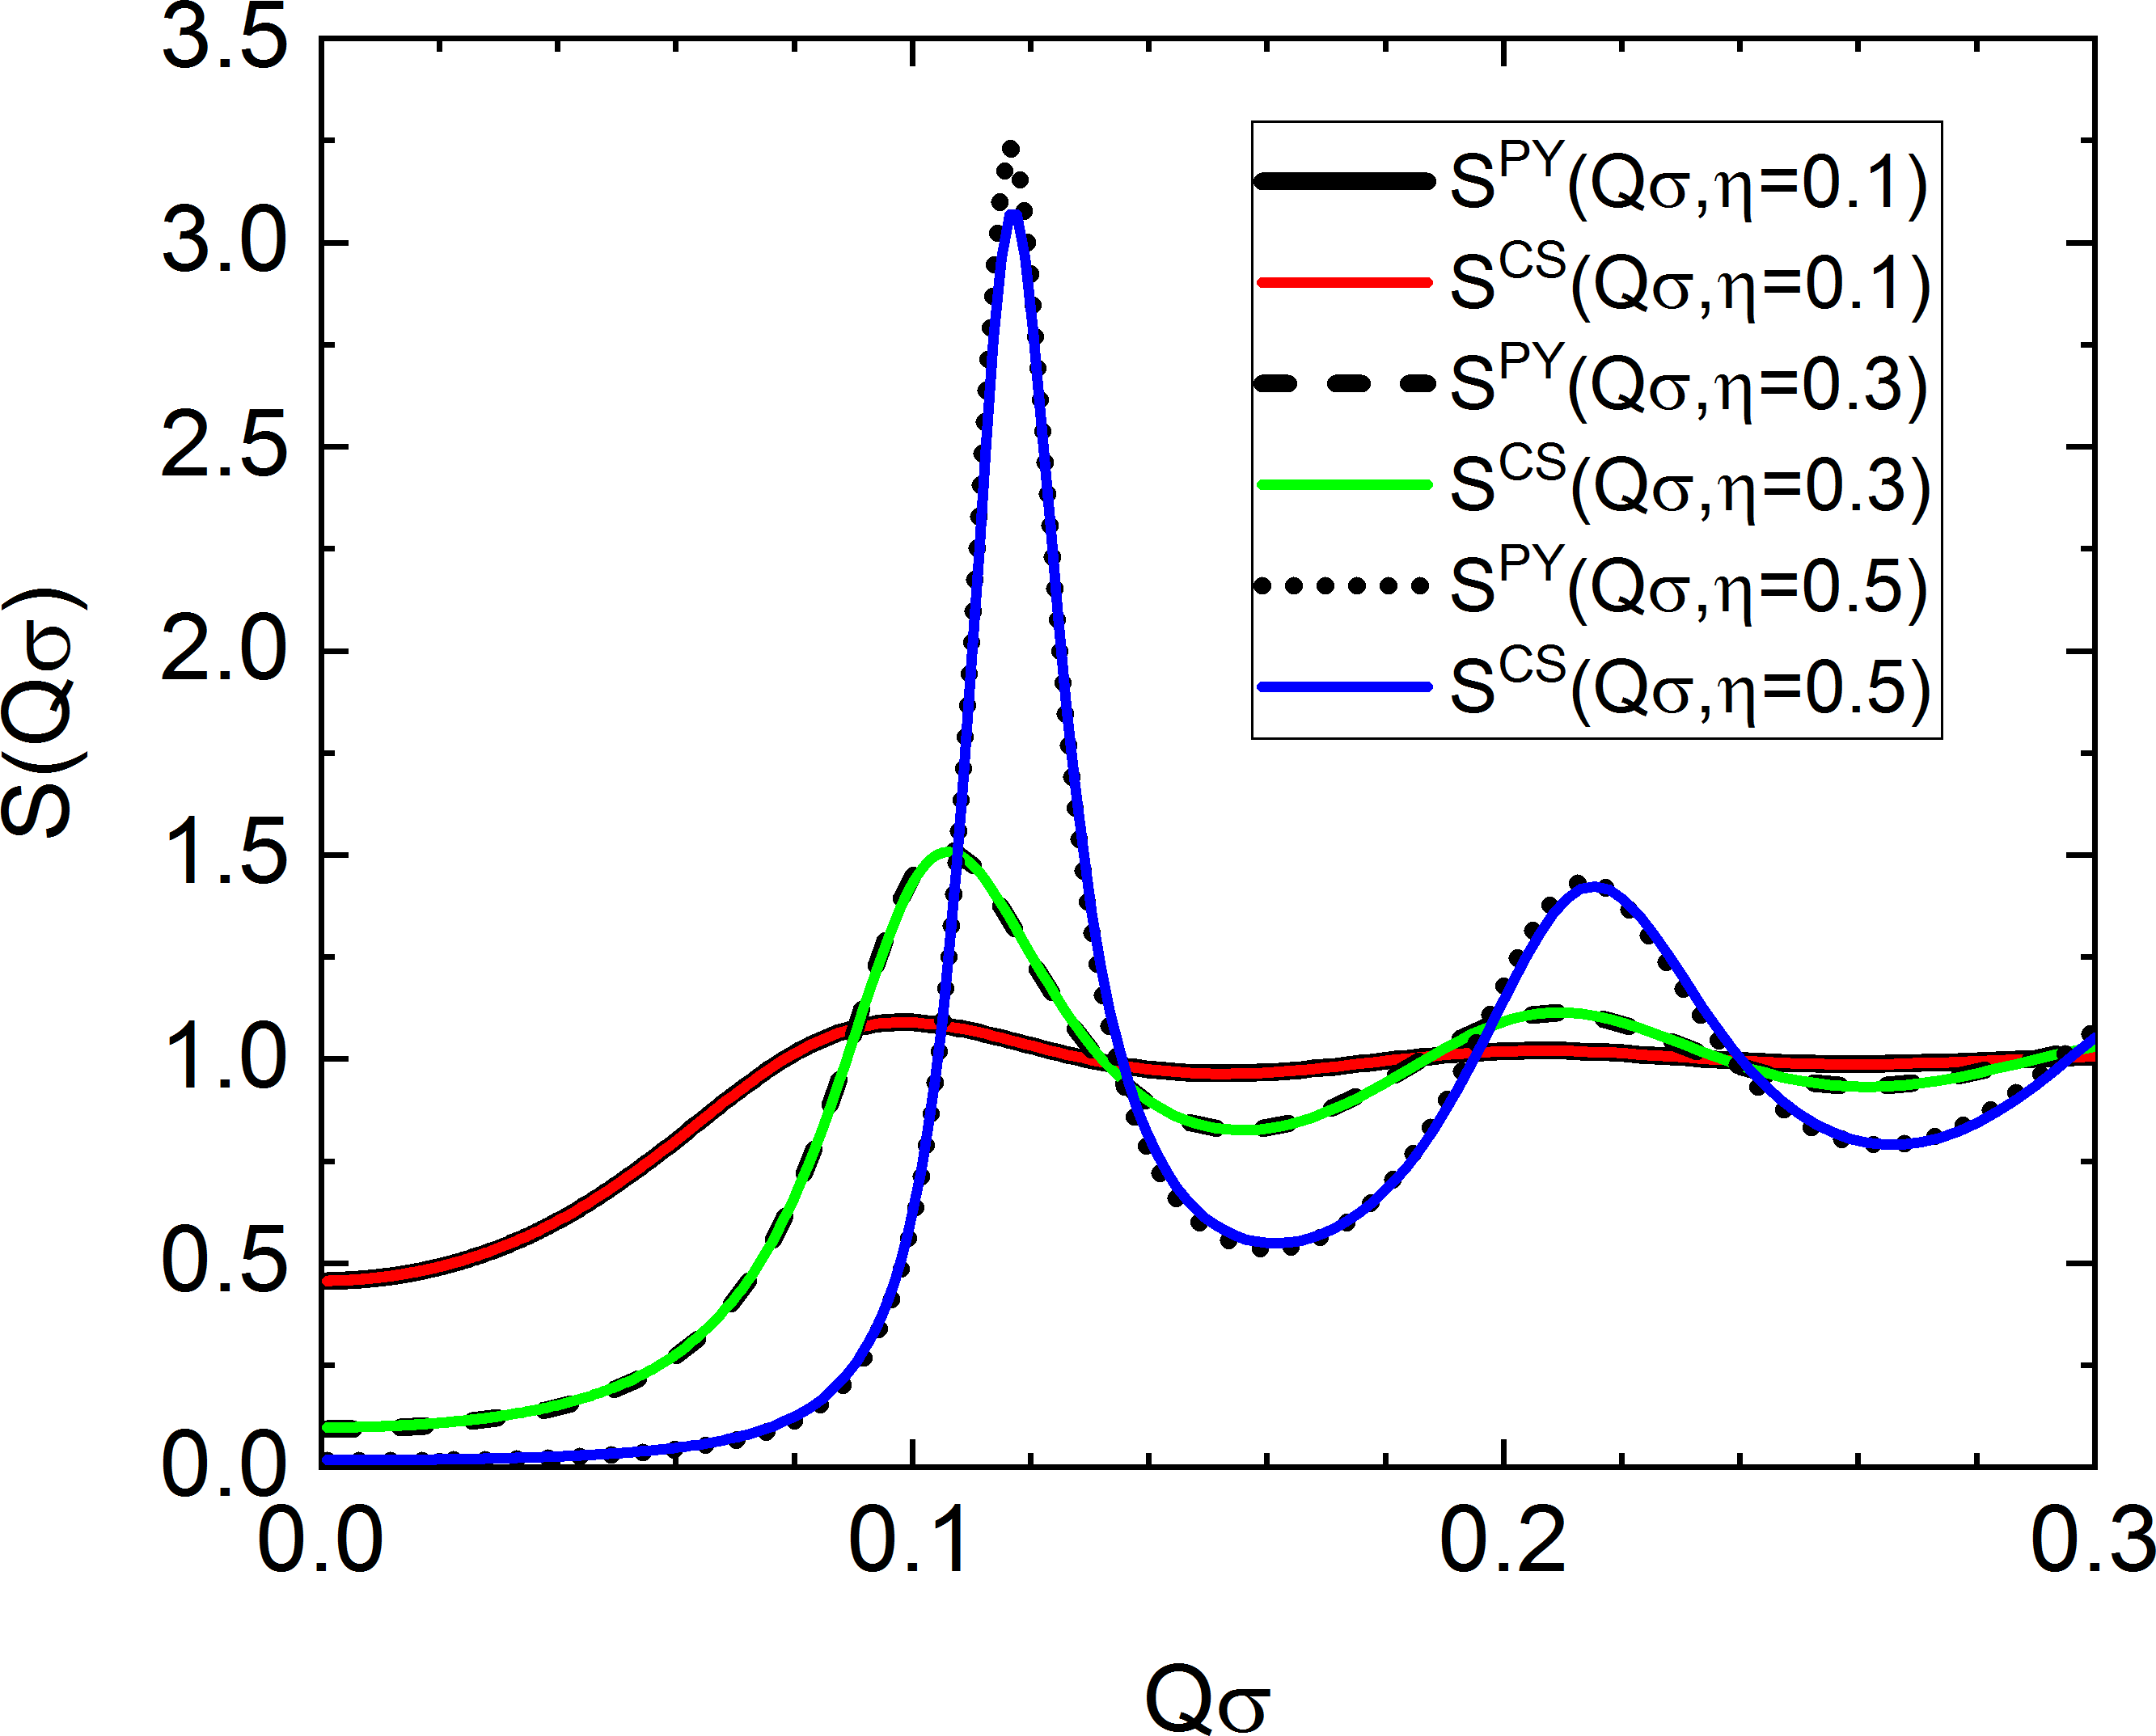
\includegraphics[width=1\textwidth]{../images/structure_factor/HardSphere/SQCS.png}
   \caption{Comparison between $S^\mathrm{PY}$ and $S^\mathrm{CS}$}
   \label{fig:SQ:CS1}
\end{subfigure}
\hfill
\begin{subfigure}[b]{.48\textwidth}
   \centering
   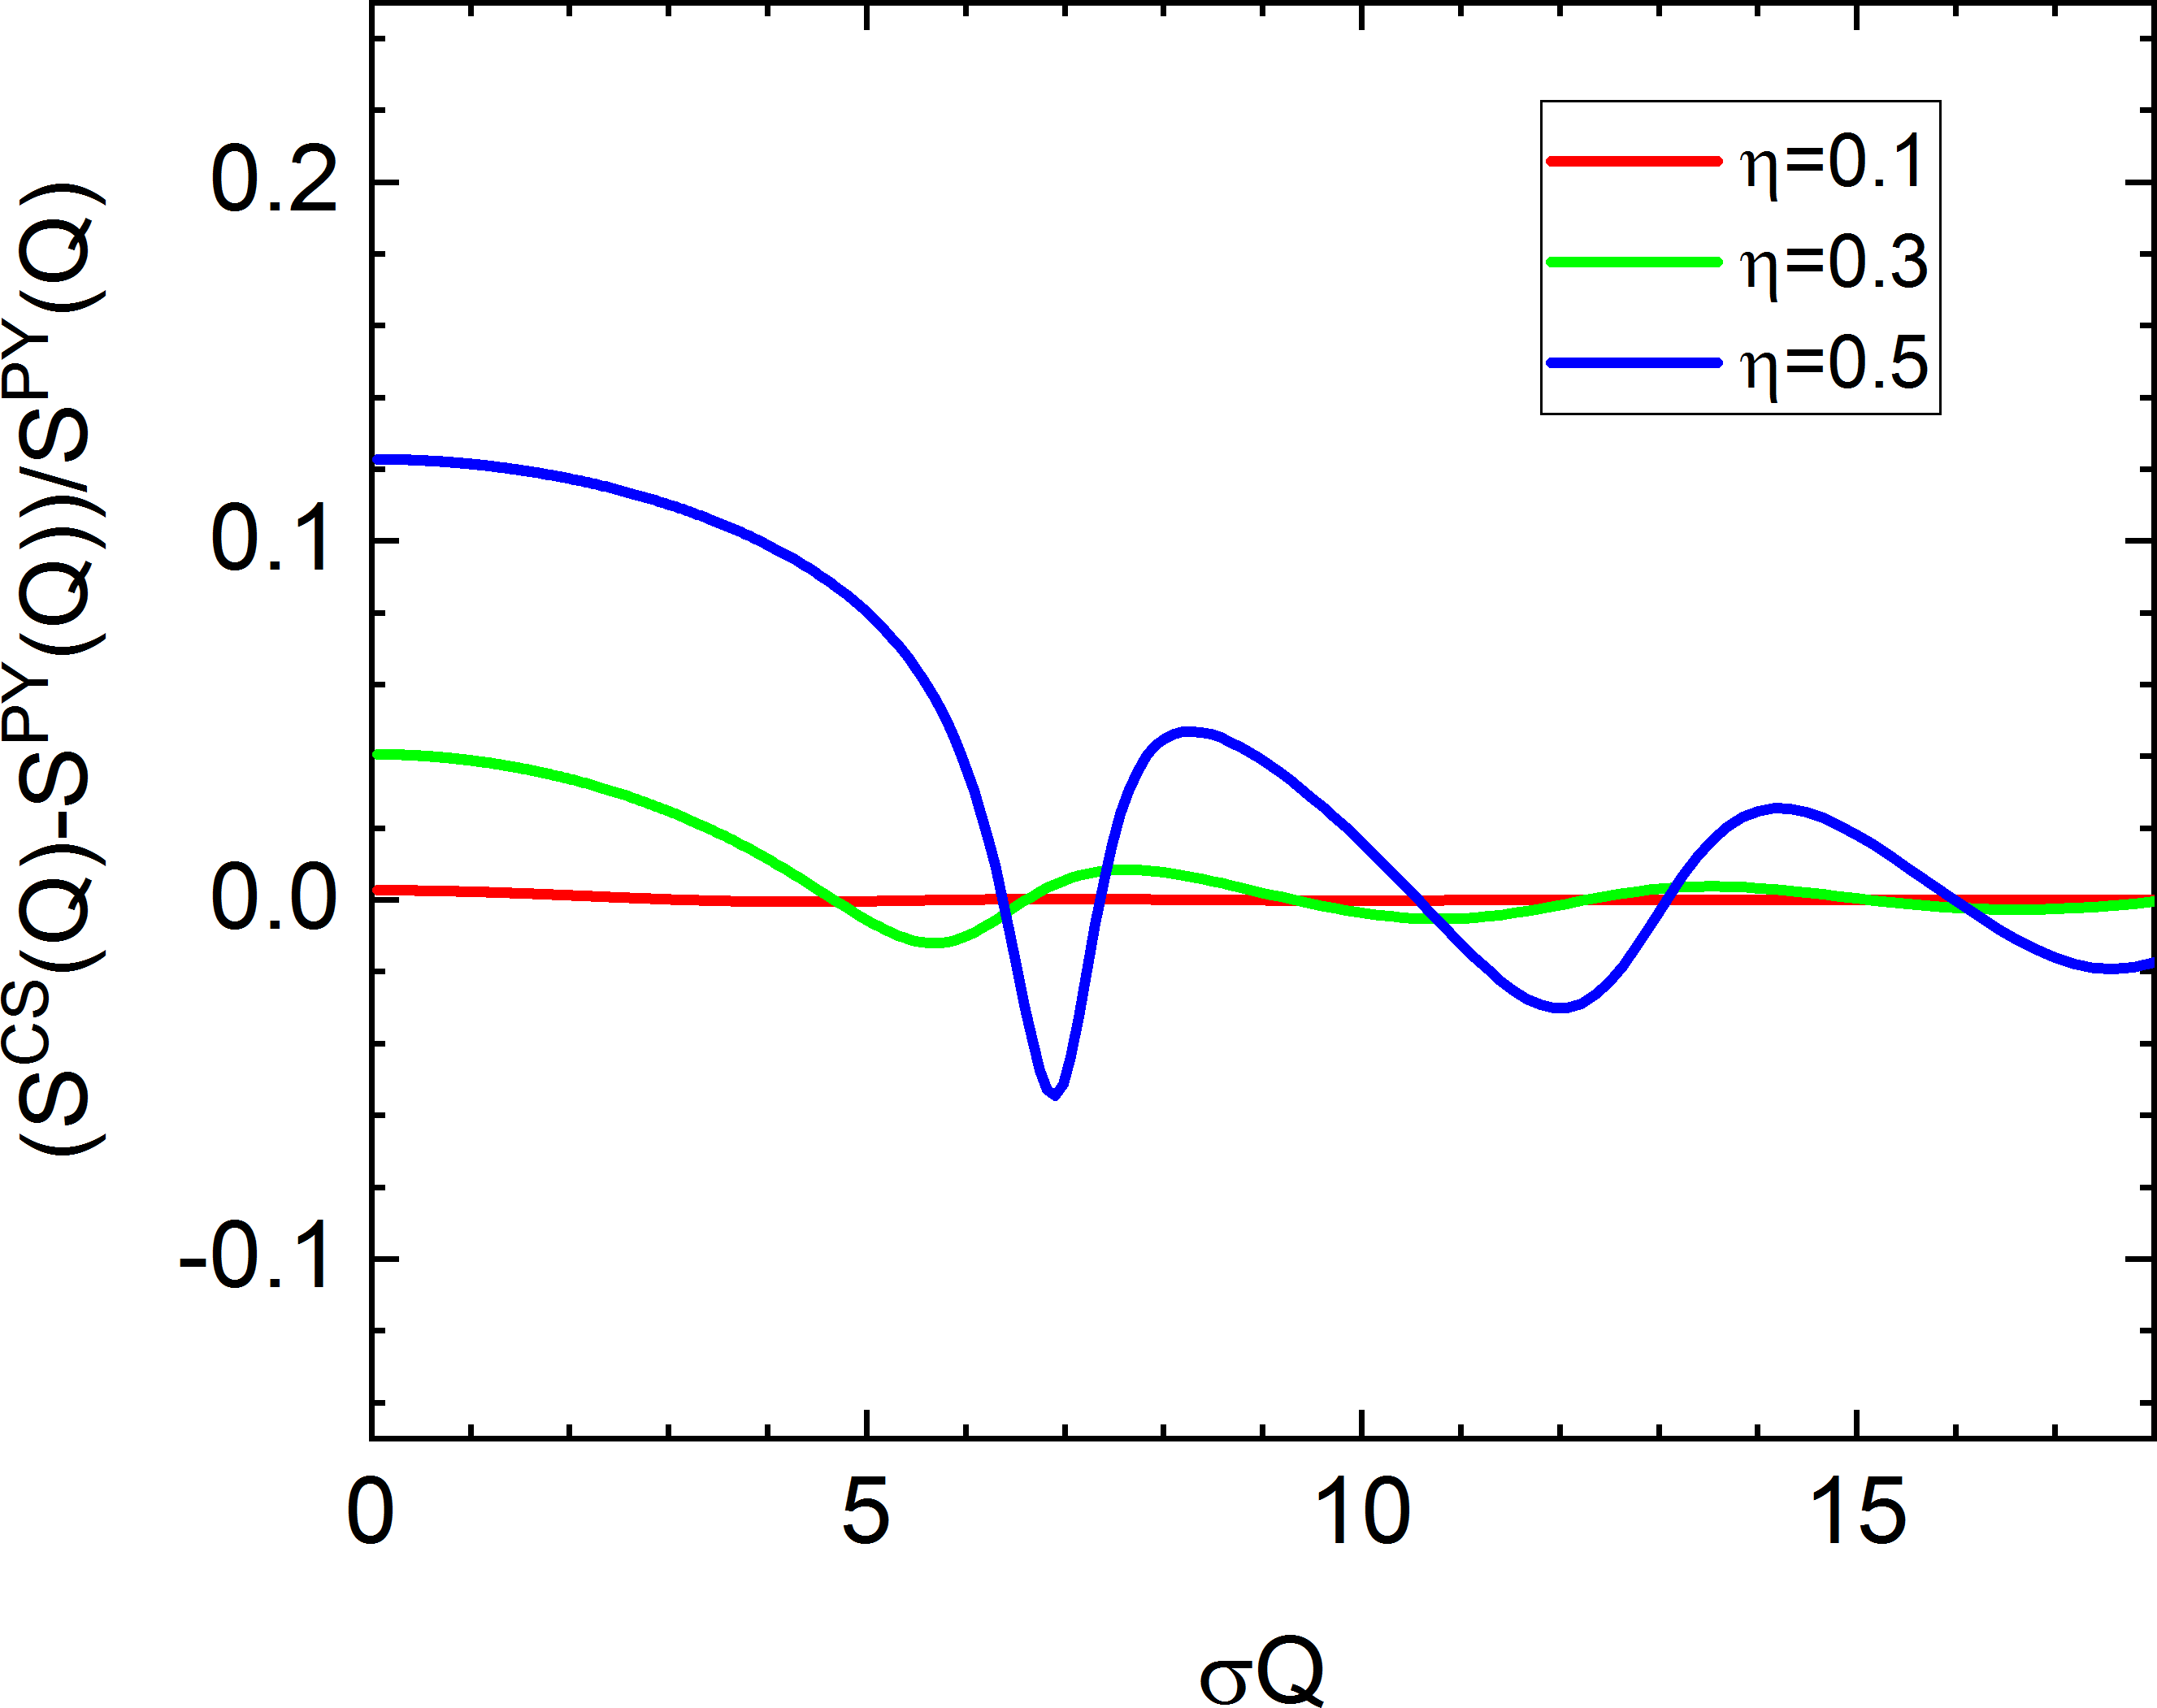
\includegraphics[width=1\textwidth]{../images/structure_factor/HardSphere/ResCS.png}
   \caption{residual between $S^\mathrm{PY}$ and $S^\mathrm{CS}$}
   \label{fig:SQ:CS2}
\end{subfigure}
\caption{Comparison between analytical PY solution of hard sphere static structure factor and rational function approximation with a compressibility factor of Carnahan and Starling}
\label{fig:SQ:CS}
\end{figure}

\clearpage
\subsection{Pad\'{e}(4,3) of van Rensburg and S\'{a}nchez} \cite{Rensburg1993,Sanchez1994} ~\\

\noindent In this approximation eqs.\ \ref{eq:RFAstart}-\ref{eq:RFAend} are used with $Z=Z^{(4,3)}$, where
\begin{align}
Z^{(4,3)} &= \frac{1+1.024385\eta+1.104537\eta^2-0.4611472\eta^3-0.7430382\eta^4}{1-2.975615\eta+3.007000\eta^2-1.097758\eta^3}
\end{align}

\vspace{5mm}

\hspace{1pt}\\
\uline{Input parameters for \texttt{3D Hard Sphere (4,3)}:}
\begin{description}
    \item[\texttt{R}]  radius $R$
    \item[\texttt{eta}] volume fraction $\eta$
\end{description}

\noindent
\uline{Note}
\begin{itemize}
\item The structure factor accepts volume fractions between $\eta \in [0,1]$.
\item The threshold packing fraction (packing
fraction at which a glass transition in the hard-sphere fluid takes place) of this model is $\eta^{(4,3)}_0 = 0.5604$  beyond
which no meaningful fluid structure can be derived \cite{Haro2004}.
\end{itemize}

\begin{figure}[htb]
\begin{subfigure}[b]{.48\textwidth}
   \centering
   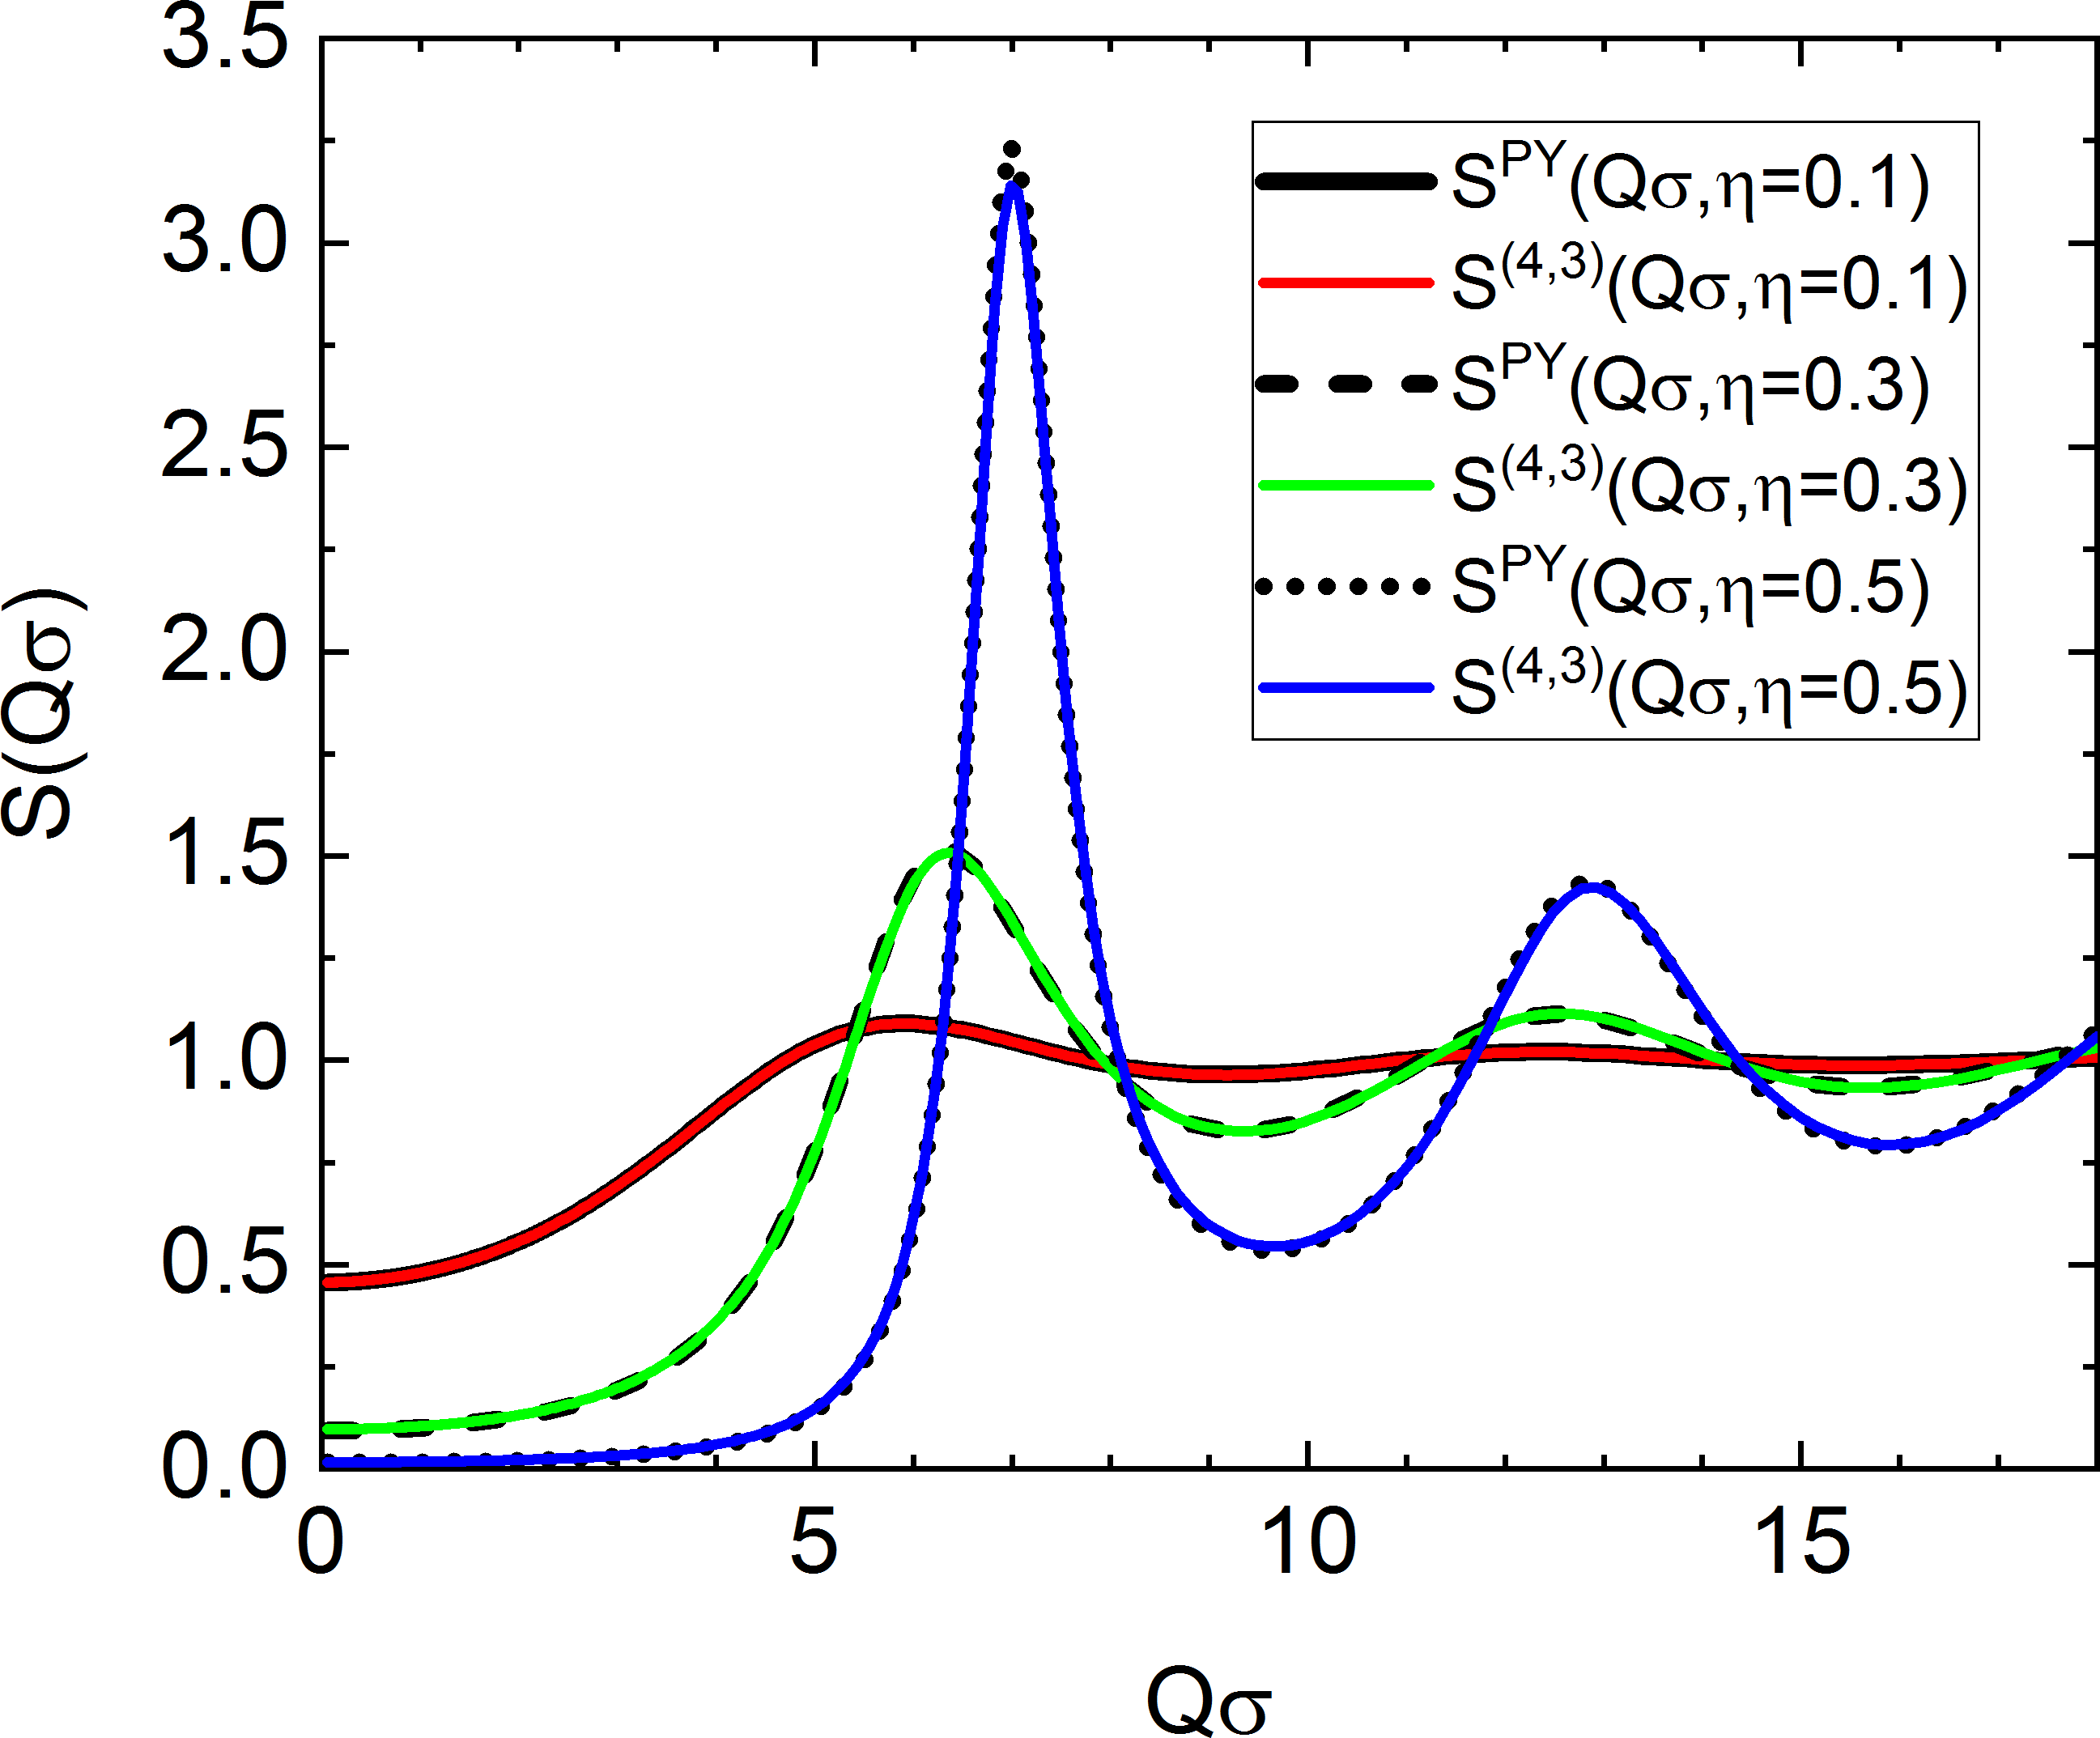
\includegraphics[width=1\textwidth]{../images/structure_factor/HardSphere/SQ(4,3).png}
   \caption{Comparison between $S^\mathrm{PY}$ and $S^{(4,3)}$}
   \label{fig:SQ:43_1}
\end{subfigure}
\hfill
\begin{subfigure}[b]{.48\textwidth}
   \centering
   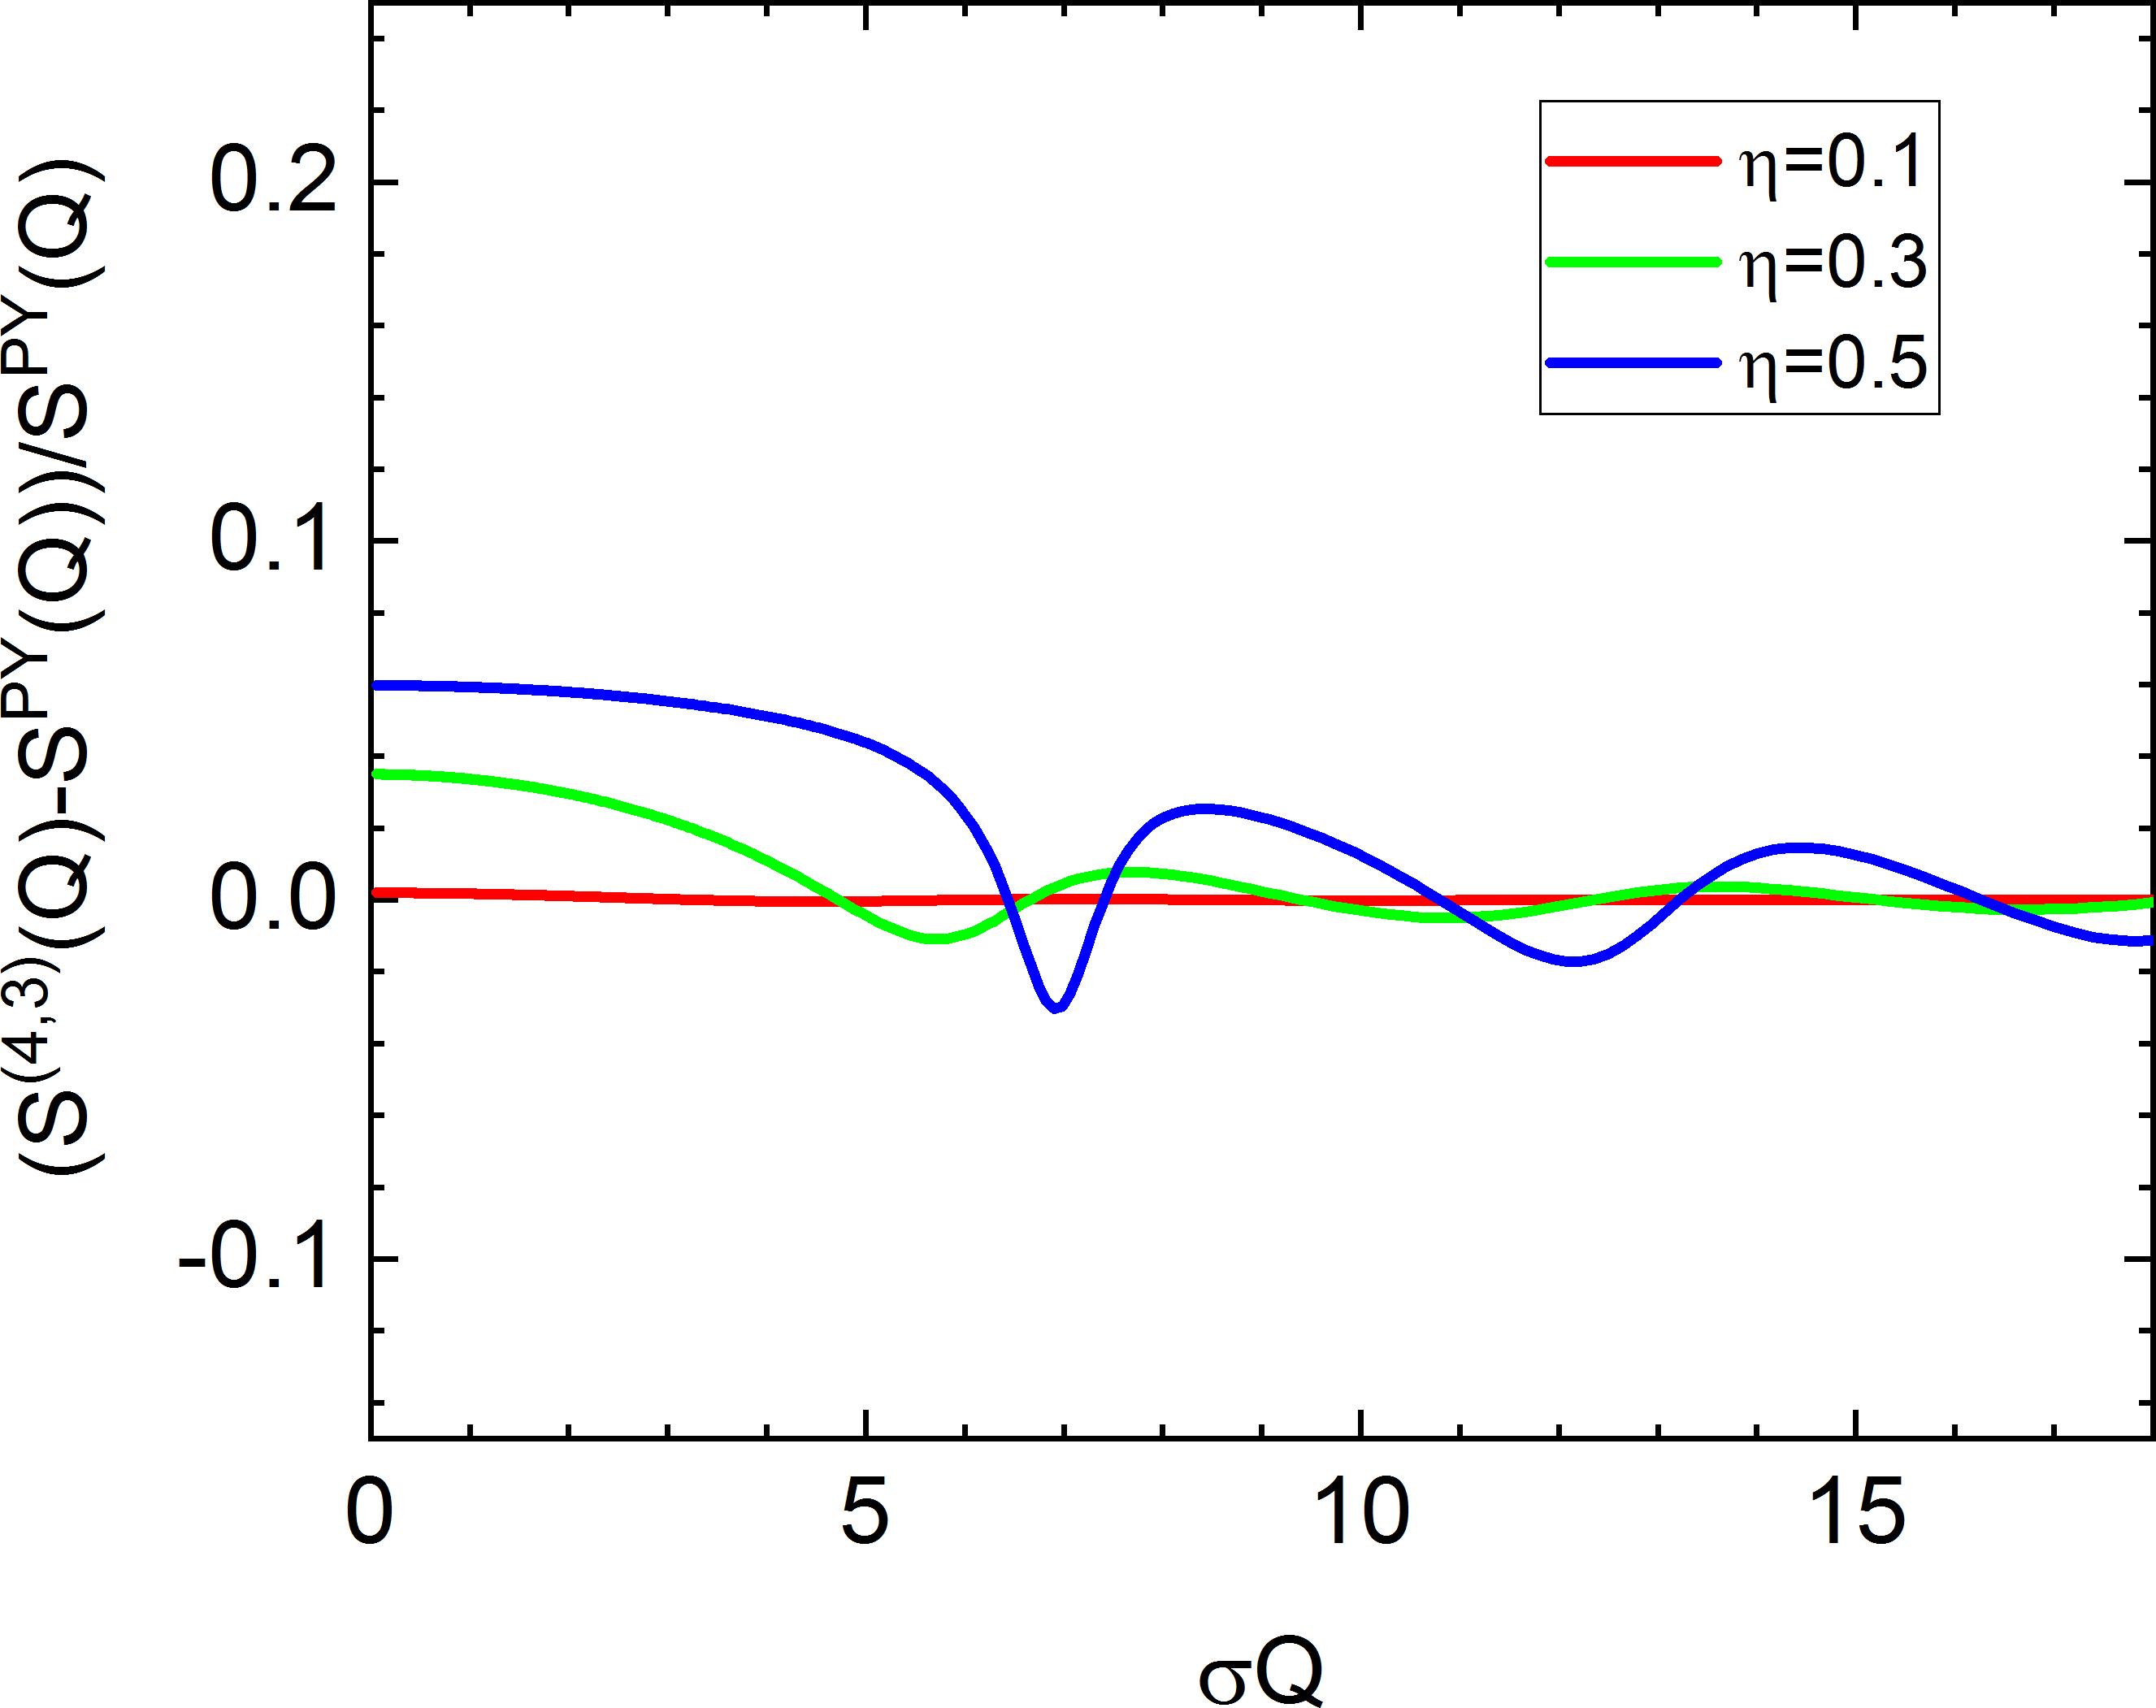
\includegraphics[width=1\textwidth]{../images/structure_factor/HardSphere/Res(4,3).png}
   \caption{residual between $S^\mathrm{PY}$ and $S^{(4,3)}$}
   \label{fig:SQ:43_2}
\end{subfigure}
\caption{Comparison between analytical PY solution of hard sphere static structure factor and rational function approximation with a compressibility factor of van Rensburg and S\'{a}nchez}
\label{fig:SQ:43}
\end{figure}

\clearpage
\subsection{Malijevsk\'{y} and Veverka} \cite{Malijevsky1999} ~\\

\noindent In this approximation eqs.\ \ref{eq:RFAstart}-\ref{eq:RFAend} are used with $Z=Z^\mathrm{MV}$, where
\begin{align}
Z^\mathrm{MV} &= \frac{1 + 1.0560\eta + 1.6539\eta^2 + 0.3262\eta^3}{\left(1- 3.8464\eta + 4.9574\eta^2 -2.1639\eta^3\right)\left(1-\eta\right)^3}
\end{align}

\vspace{5mm}

\hspace{1pt}\\
\uline{Input parameters for \texttt{3D Hard Sphere (MV)}:}
\begin{description}
    \item[\texttt{R}]  radius $R$
    \item[\texttt{eta}] volume fraction $\eta$
\end{description}

\noindent
\uline{Note}
\begin{itemize}
\item The structure factor accepts volume fractions between $\eta \in [0,1]$.
\item The model lead to physically meaningful structural properties in the whole definition range of volume fractions.
\end{itemize}

\begin{figure}[htb]
\begin{subfigure}[b]{.48\textwidth}
   \centering
   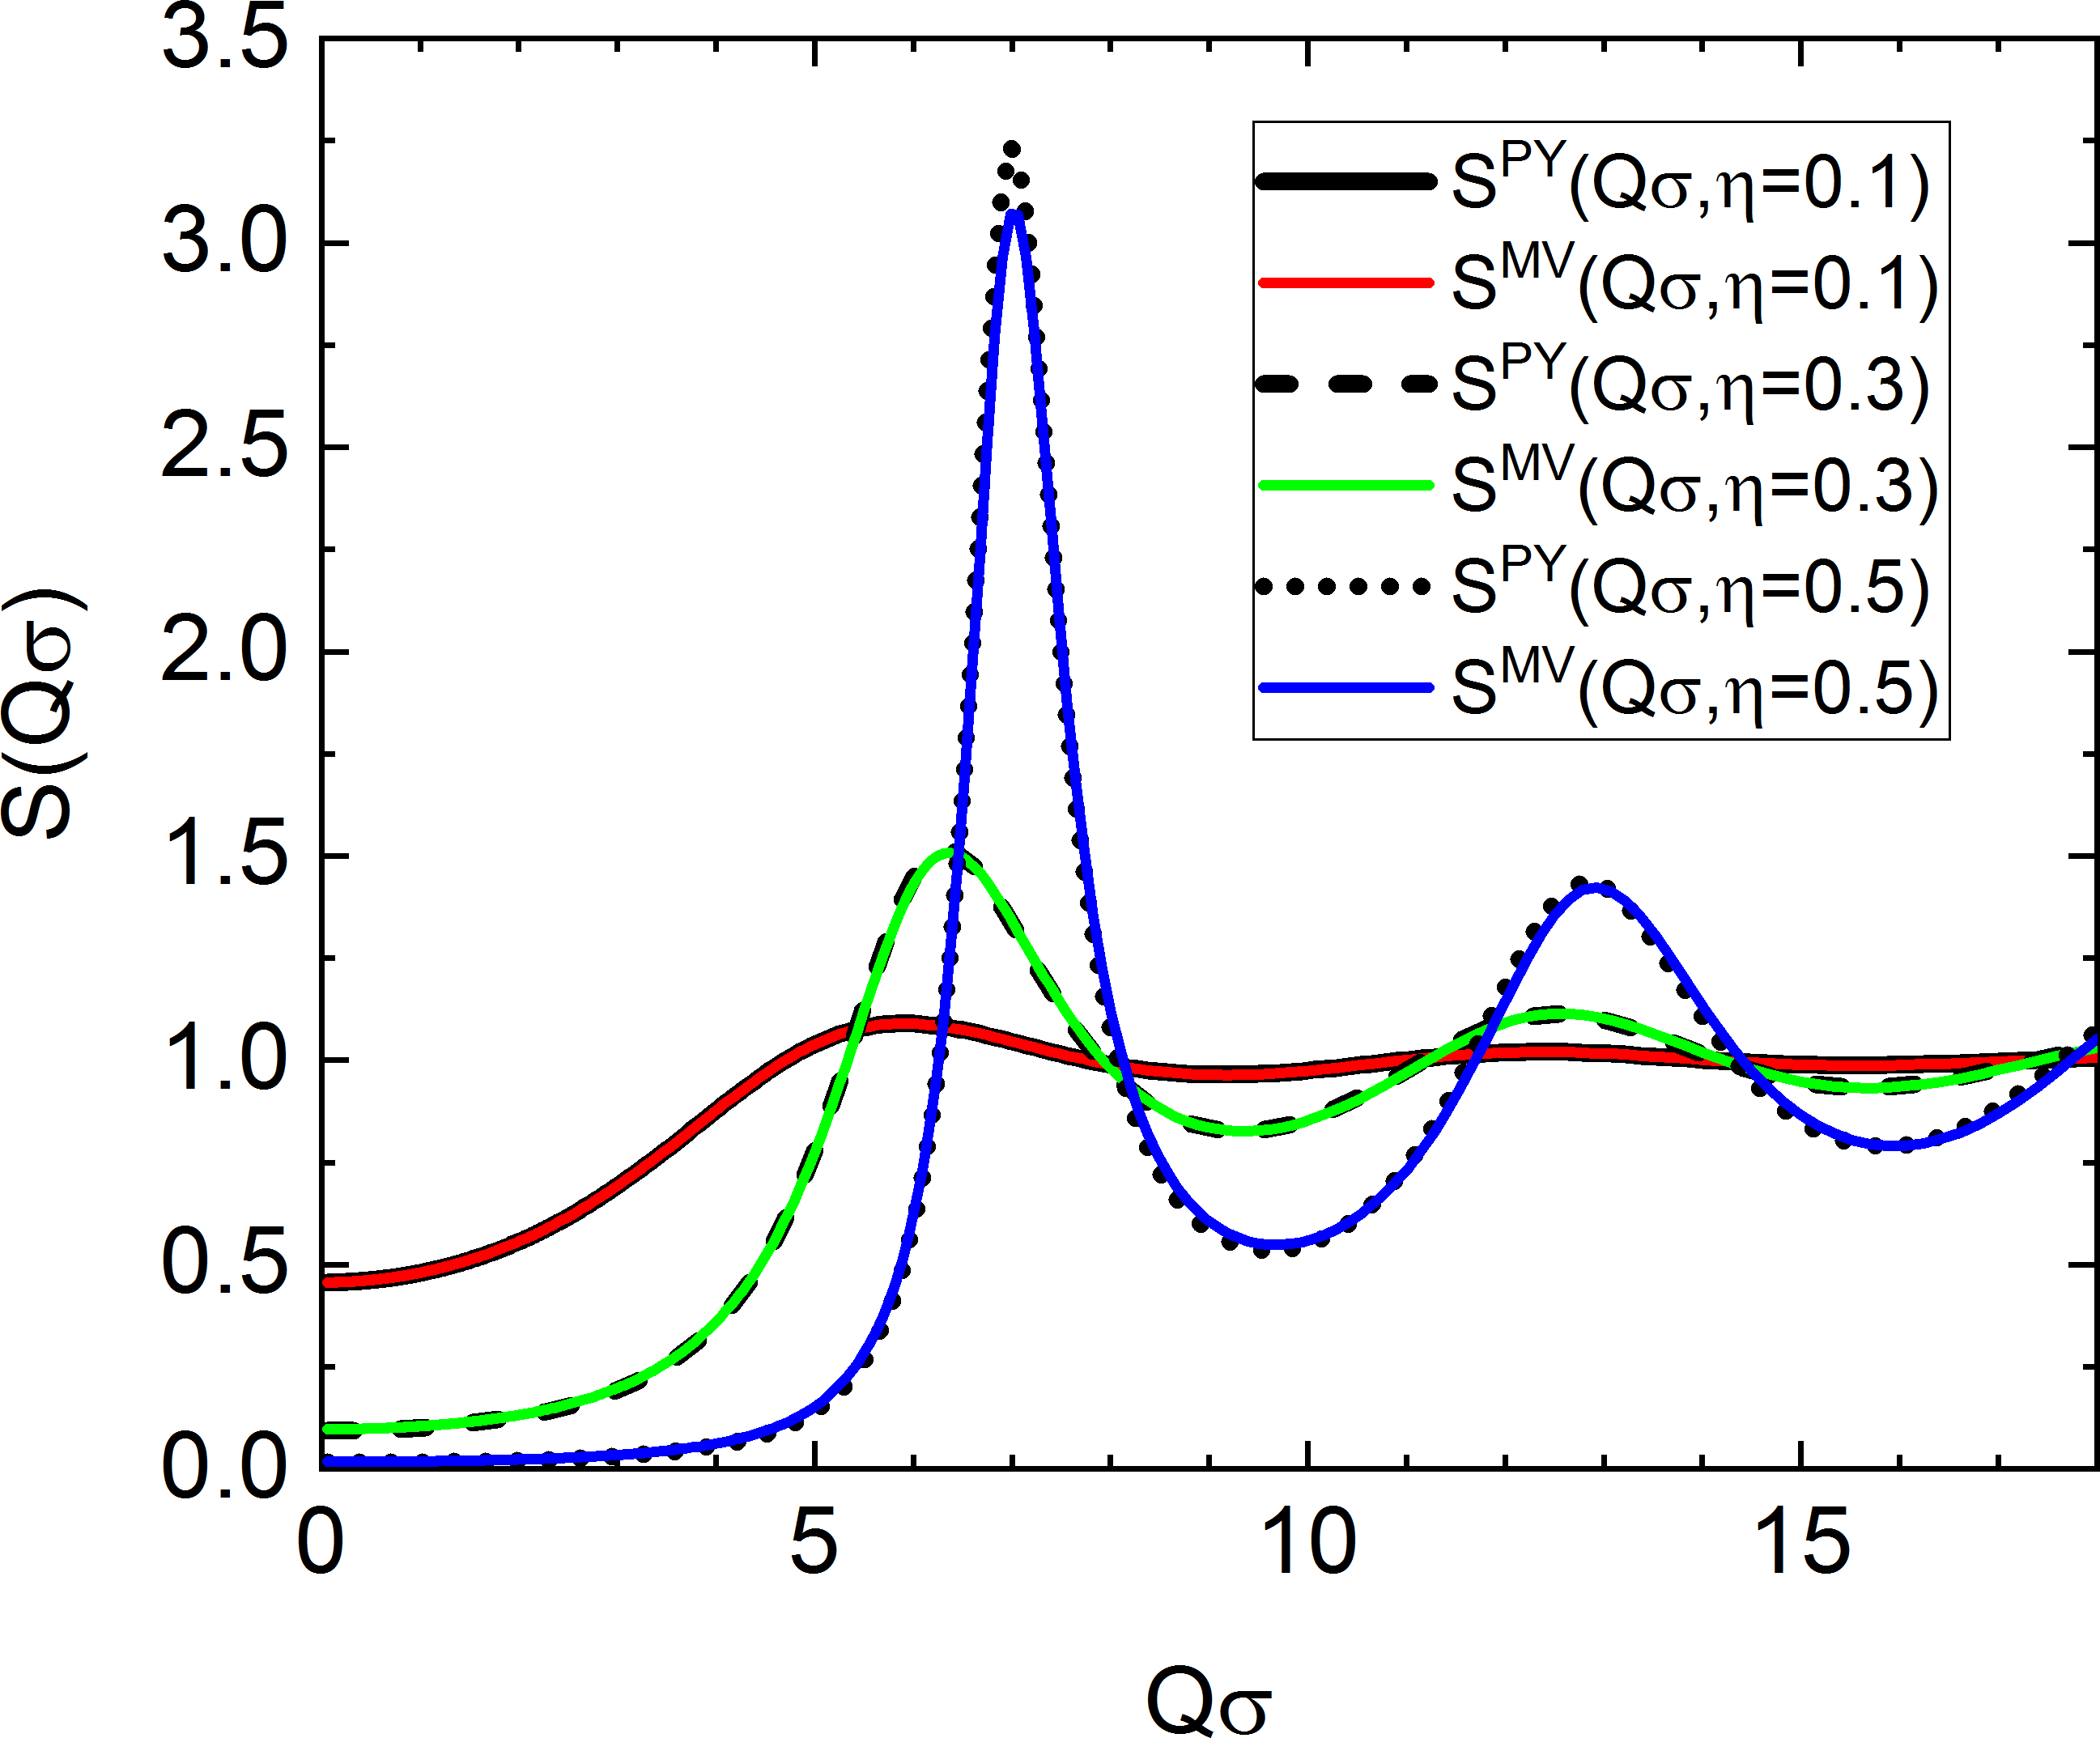
\includegraphics[width=1\textwidth]{../images/structure_factor/HardSphere/SQMV.png}
   \caption{Comparison between $S^\mathrm{PY}$ and $S^\mathrm{MV}$}
   \label{fig:SQ:MV_1}
\end{subfigure}
\hfill
\begin{subfigure}[b]{.48\textwidth}
   \centering
   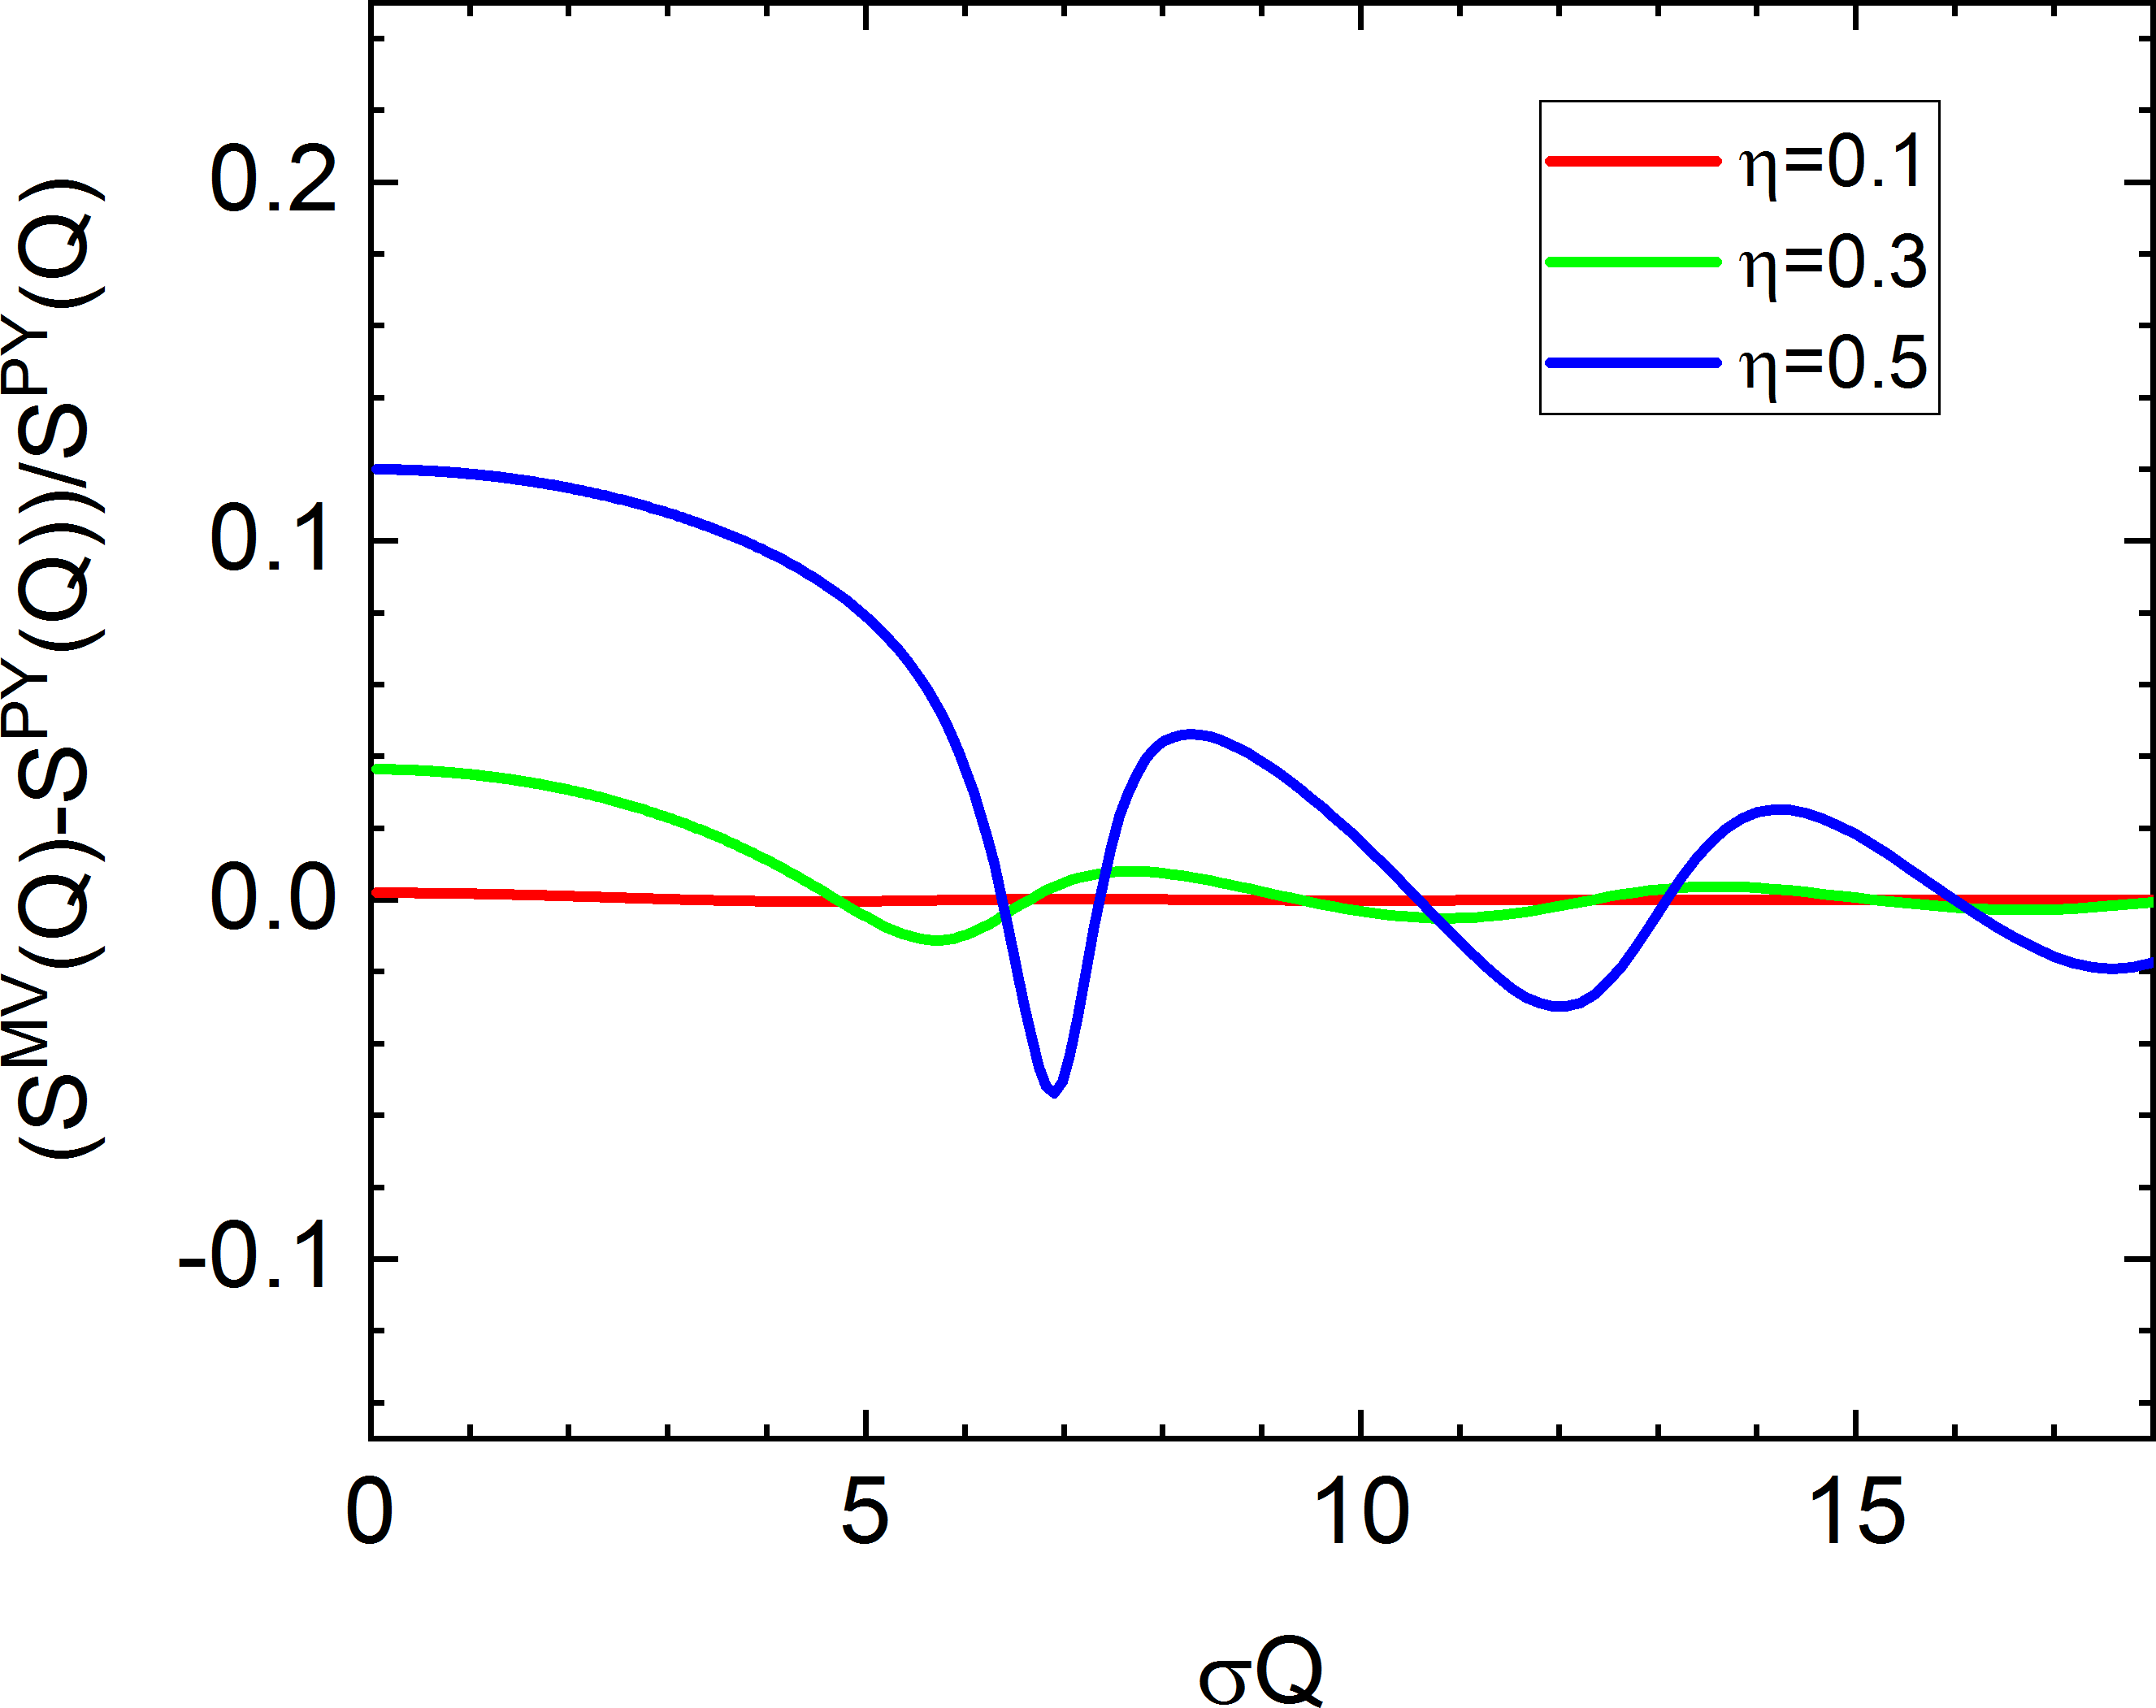
\includegraphics[width=1\textwidth]{../images/structure_factor/HardSphere/ResMV.png}
   \caption{residual between $S^\mathrm{PY}$ and $S^\mathrm{MV}$}
   \label{fig:SQ:MV_2}
\end{subfigure}
\caption{Comparison between analytical PY solution of hard sphere static structure factor and rational function approximation with a compressibility factor of Malijevsk\'{y} and Veverka}
\label{fig:SQ:MV}
\end{figure}

\clearpage
\subsection{L\'{o}pez de Haro and Robles} \cite{Robles2003} ~\\

\noindent In this approximation eqs.\ \ref{eq:RFAstart}-\ref{eq:RFAend} are used with $Z=Z^\mathrm{LHR}$, where
\begin{align}
Z^\mathrm{LHR} &= \frac{1   + 0.153555\eta
                            - 0.428376\eta^2
                            - 2.7987\eta^3
                            - 0.317417\eta^4
                            - 0.105806\eta^5}{1-3.84644\eta + 4.9574\eta^2 - 2.16386\eta^3}
\end{align}

\vspace{5mm}

\hspace{1pt}\\
\uline{Input parameters for \texttt{3D Hard Sphere (LHR)}:}
\begin{description}
    \item[\texttt{R}]  radius $R$
    \item[\texttt{eta}] volume fraction $\eta$
\end{description}

\noindent
\uline{Note}
\begin{itemize}
\item The structure factor accepts volume fractions between $\eta \in [0,1]$.
\item The threshold packing fraction (packing
fraction at which a glass transition in the hard-sphere fluid takes place) of this model is $\eta^\mathrm{LHR}_0 = 0.5684$  beyond
which no meaningful fluid structure can be derived \cite{Haro2004}.
\end{itemize}

\begin{figure}[htb]
\begin{subfigure}[b]{.48\textwidth}
   \centering
   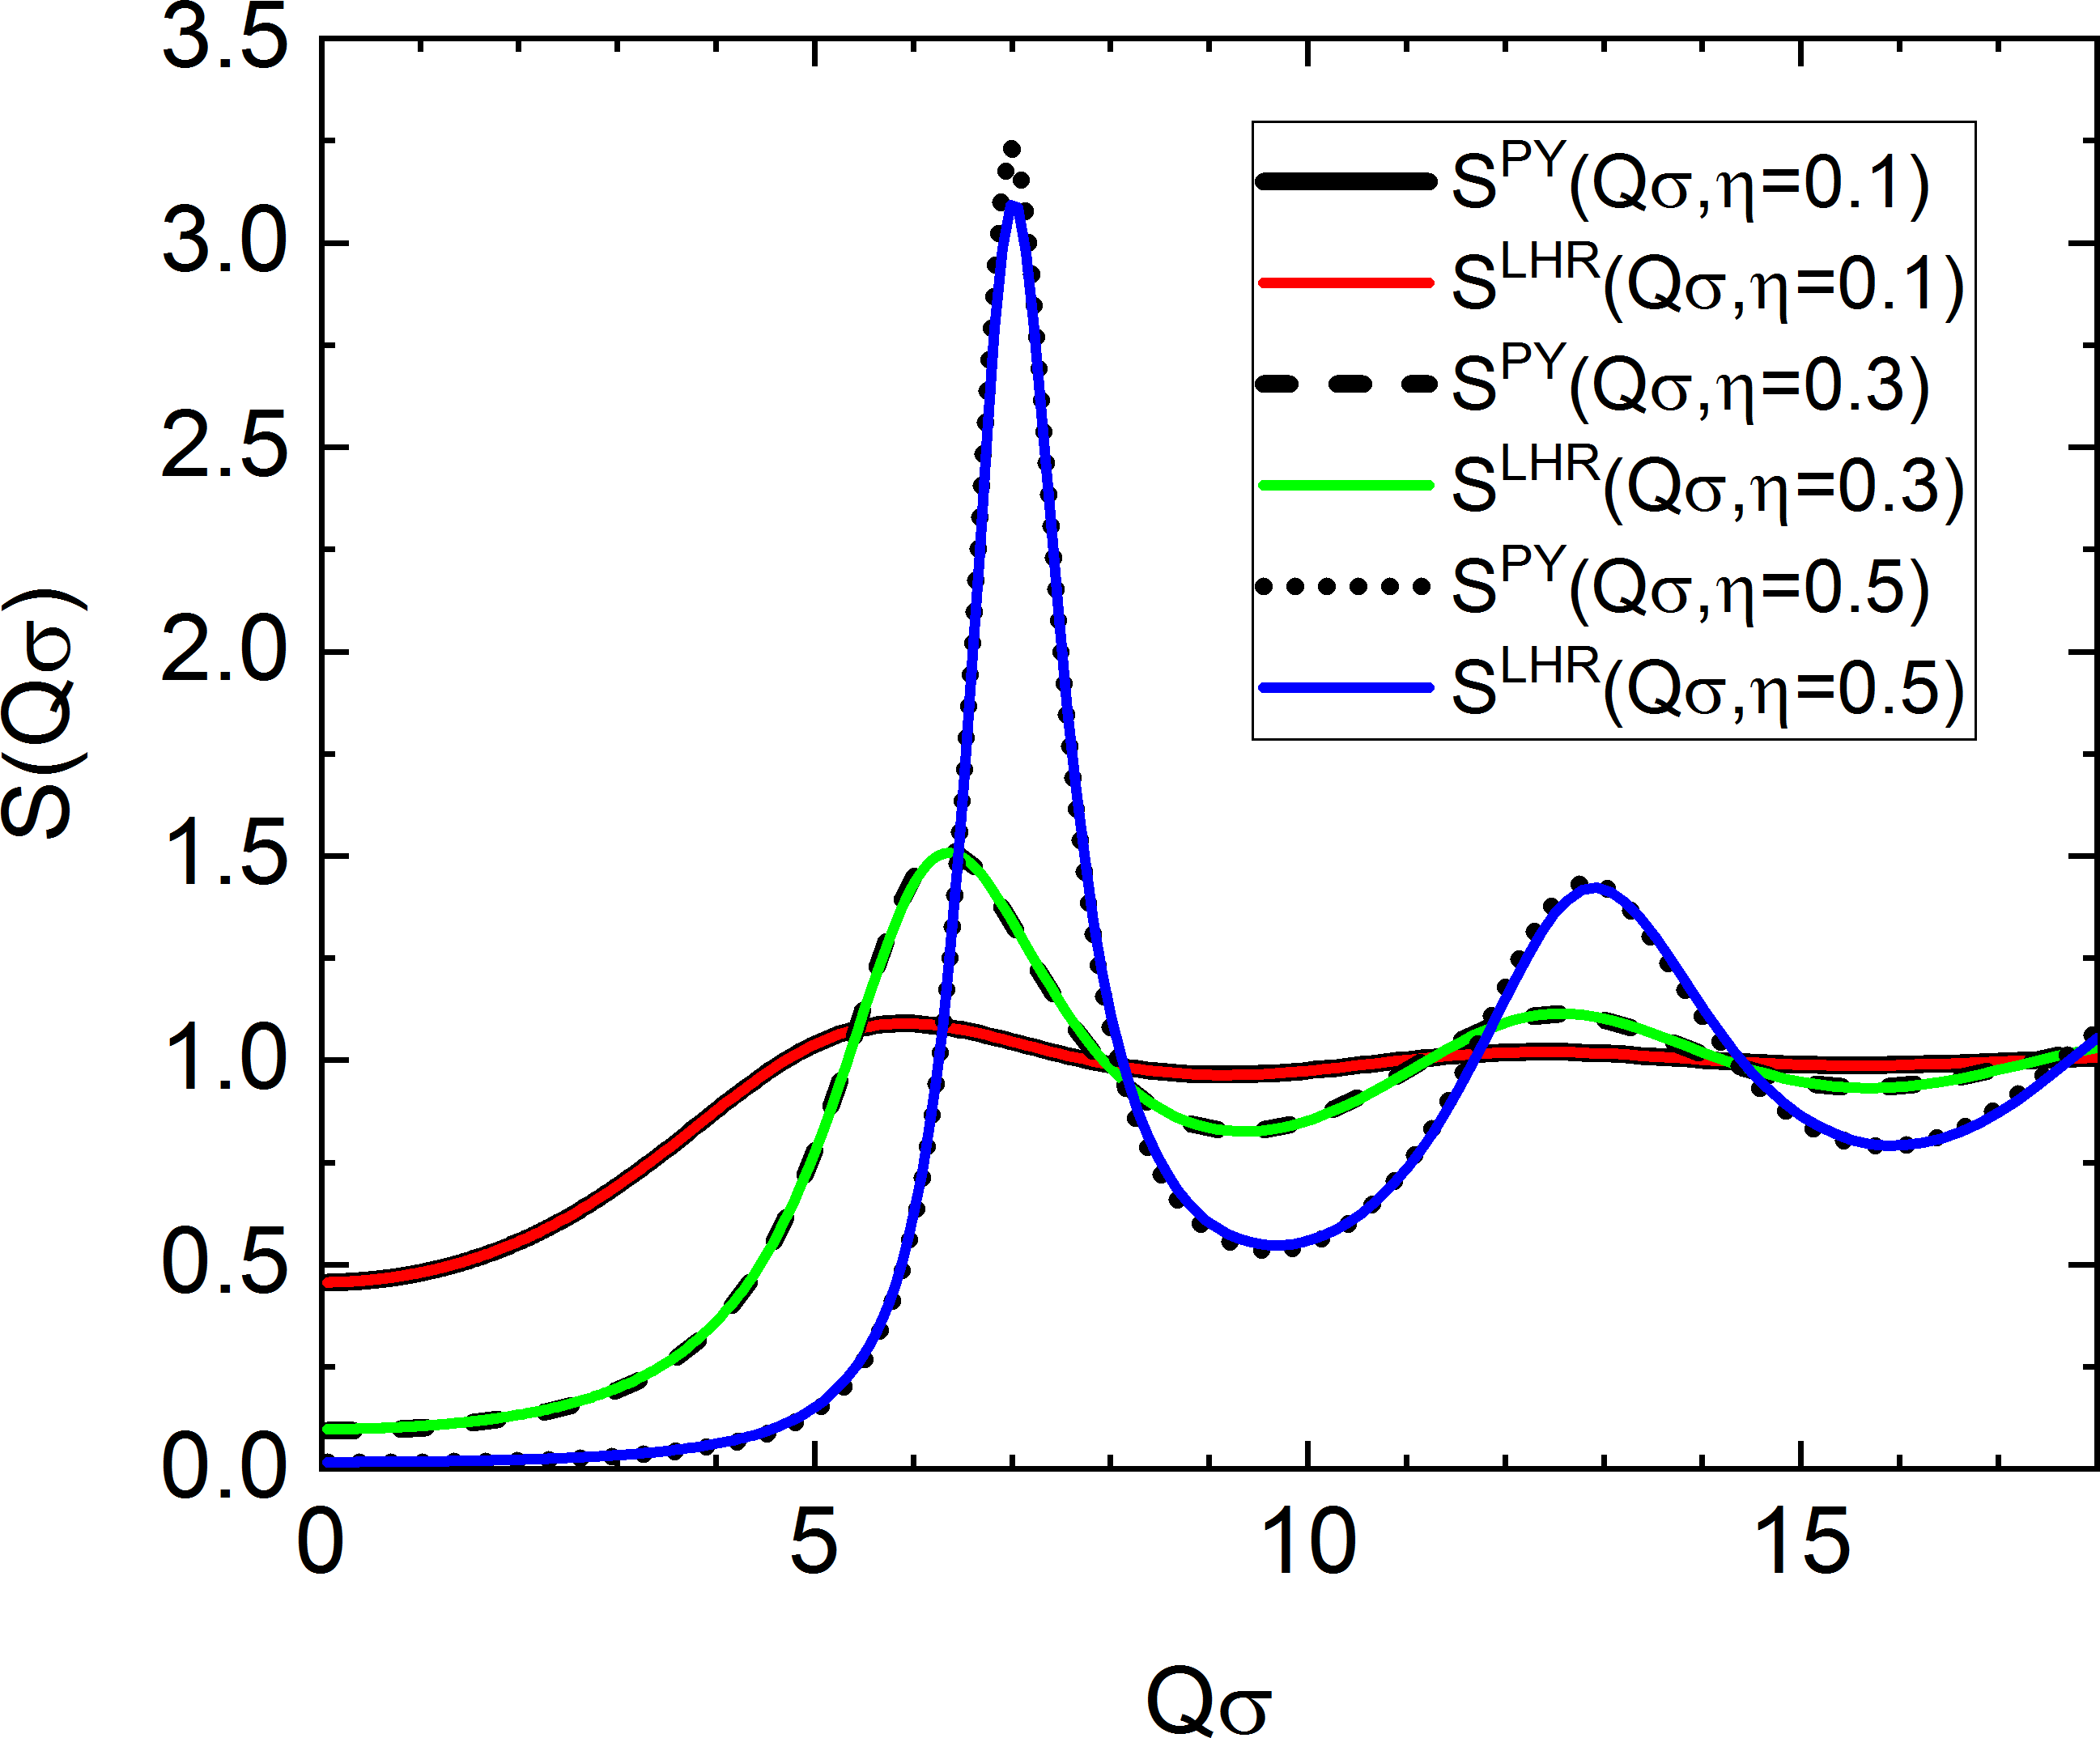
\includegraphics[width=1\textwidth]{../images/structure_factor/HardSphere/SQLHR.png}
   \caption{Comparison between $S^\mathrm{PY}$ and $S^\mathrm{LHR}$}
   \label{fig:SQ:LHR_1}
\end{subfigure}
\hfill
\begin{subfigure}[b]{.48\textwidth}
   \centering
   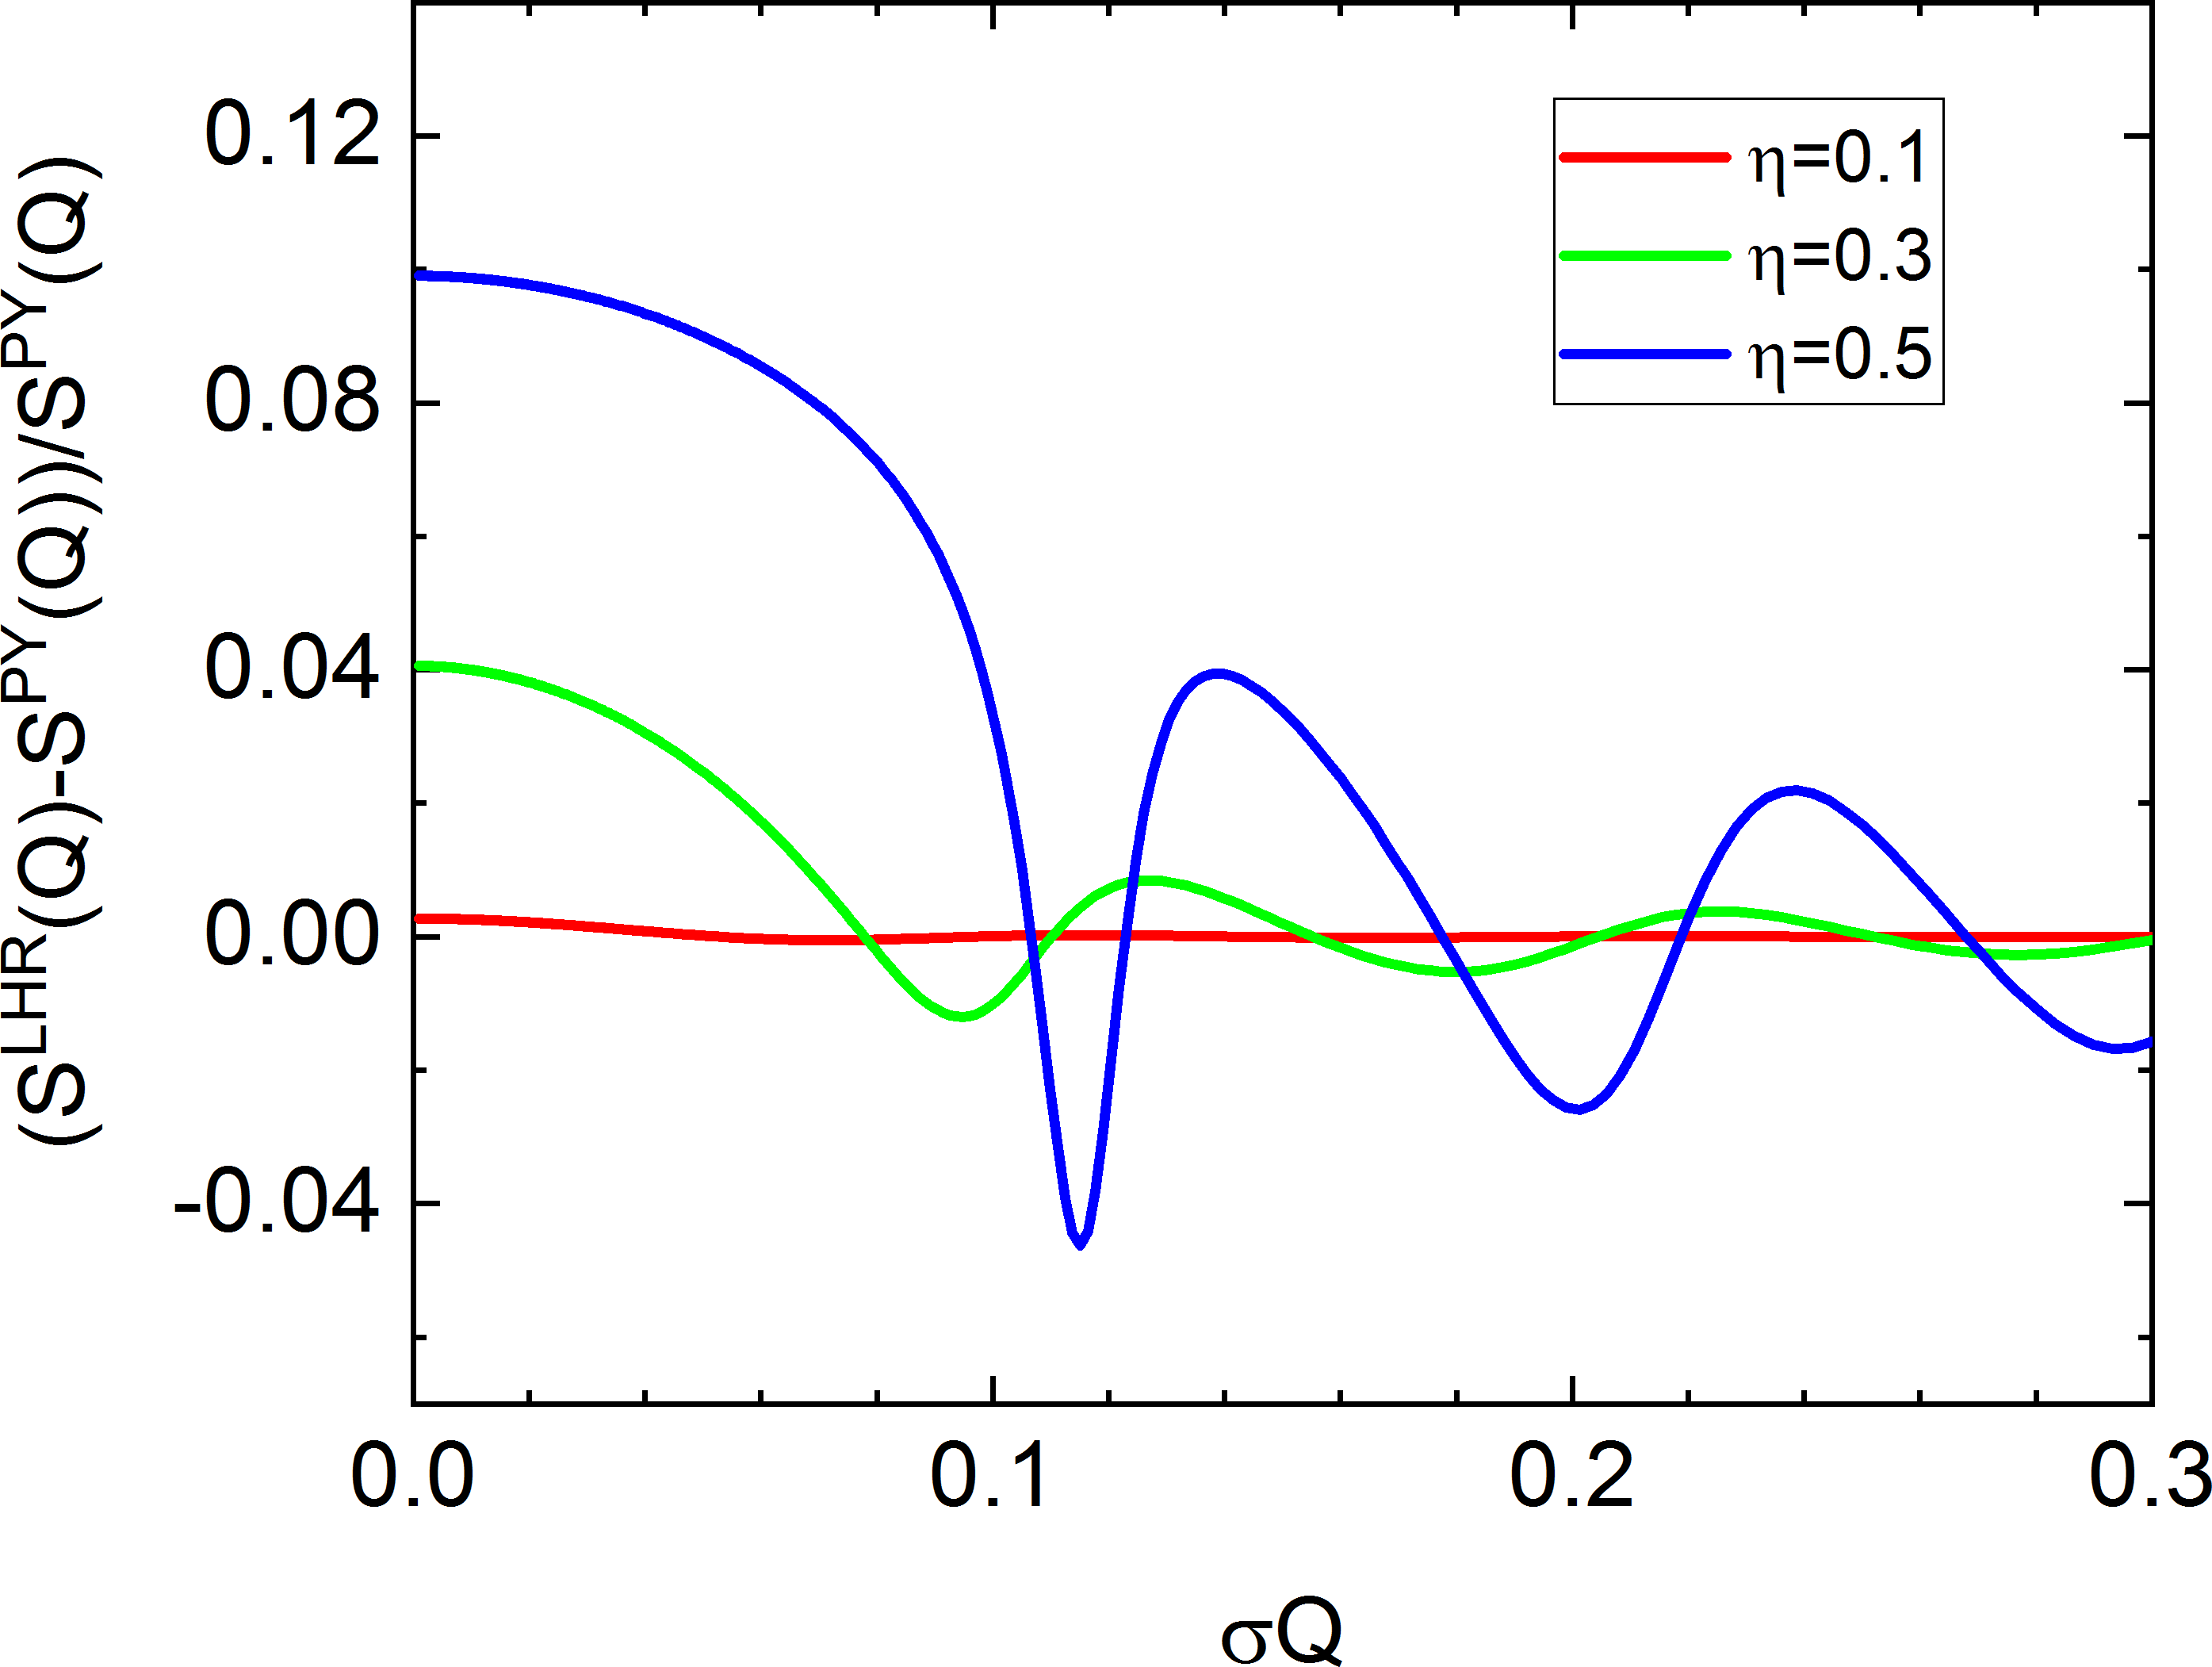
\includegraphics[width=1\textwidth]{../images/structure_factor/HardSphere/ResLHR.png}
   \caption{residual between $S^\mathrm{PY}$ and $S^\mathrm{LHR}$}
   \label{fig:SQ:LHR_2}
\end{subfigure}
\caption{Comparison between analytical PY solution of hard sphere static structure factor and rational function approximation with a compressibility factor of L\'{o}pez de Haro and Robles}
\label{fig:SQ:LHR}
\end{figure}

\clearpage
\subsection{Grundke and Henderson} ~\\

\noindent In this approximation the structure factor in the Percus Yevick approximation is corrected to have thermodynamic consistency \cite{Henderson1975} so that both routes leads to the expression of Carnahan and Starling
$pV/Nk_BT=\frac{1+\eta+\eta^2-\eta^3}{\left(1-\eta\right)^3}$
\begin{align}
\sigma &= 2R\\
\left(\sigma_0/\sigma\right)^3 &= 1-\eta/16\\
\eta_0 &= \eta (1-\eta/16) \\
g_0(s,\eta_0) &\simeq \frac{1+\eta_0/2}{\left(1-\eta_0\right)^2} - \frac{9}{2}\eta_0\frac{1+\eta_0}{\left(1-\eta_0\right)^3}(s-1) \\
\frac{C}{\sigma} &= \frac{2-\eta}{2(1-\eta)^3} - g_0(\sigma/\sigma_0,\eta_0) \\
\frac{12\eta C}{m\sigma_0^2} &= \frac{(1-\eta)^4}{1+4\eta+4\eta^2-4\eta^3+\eta^4} - \frac{(1-\eta_0)^4}{(1+2\eta_0)^2} \nonumber \\
&= 24\eta_0\int_0^{\sigma/\sigma_0} g_0(s,\eta_0)s^2 \mathrm{d}s \\
S^\mathrm{GH}(Q,\sigma,\eta) &= S^\mathrm{PY}(Q,\sigma_0,\eta_0) + \frac{6\eta}{\pi\sigma^3}\tilde{h}_\mathrm{GH}(Q) \\
\tilde{h}_\mathrm{GH}(Q)  &= -\frac{4\pi\sigma_0}{Q\sigma_0} \int_1^{\sigma/\sigma_0} sg_0(s,\eta_0)\sin(Q\sigma_0 s)\mathrm{d}s\\
&+ \frac{2\pi\sigma^3}{Q\sigma}\frac{C}{\sigma} \left\{ \frac{\cos (Q\sigma)}{\sigma}\left[\frac{Q+m}{m^2+(Q+m)^2}+\frac{Q-m}{m^2+(Q-m)^2}\right]\right.\nonumber \\
& + \left. \frac{\sin (Q\sigma)}{\sigma}\left[\frac{m}{m^2+(Q+m)^2}+\frac{m}{m^2+(Q-m)^2}\right]\right\}\nonumber
\end{align}

\vspace{5mm}

\hspace{1pt}\\
\uline{Input parameters for \texttt{3D Hard Sphere (GH)}:}
\begin{description}
    \item[\texttt{R}]  radius $R$
    \item[\texttt{eta}] volume fraction $\eta$
\end{description}

\noindent
\uline{Note}
\begin{itemize}
\item The structure factor accepts volume fractions between $\eta \in [0,1]$.
\end{itemize}

\begin{figure}[htb]
\begin{subfigure}[b]{.48\textwidth}
   \centering
   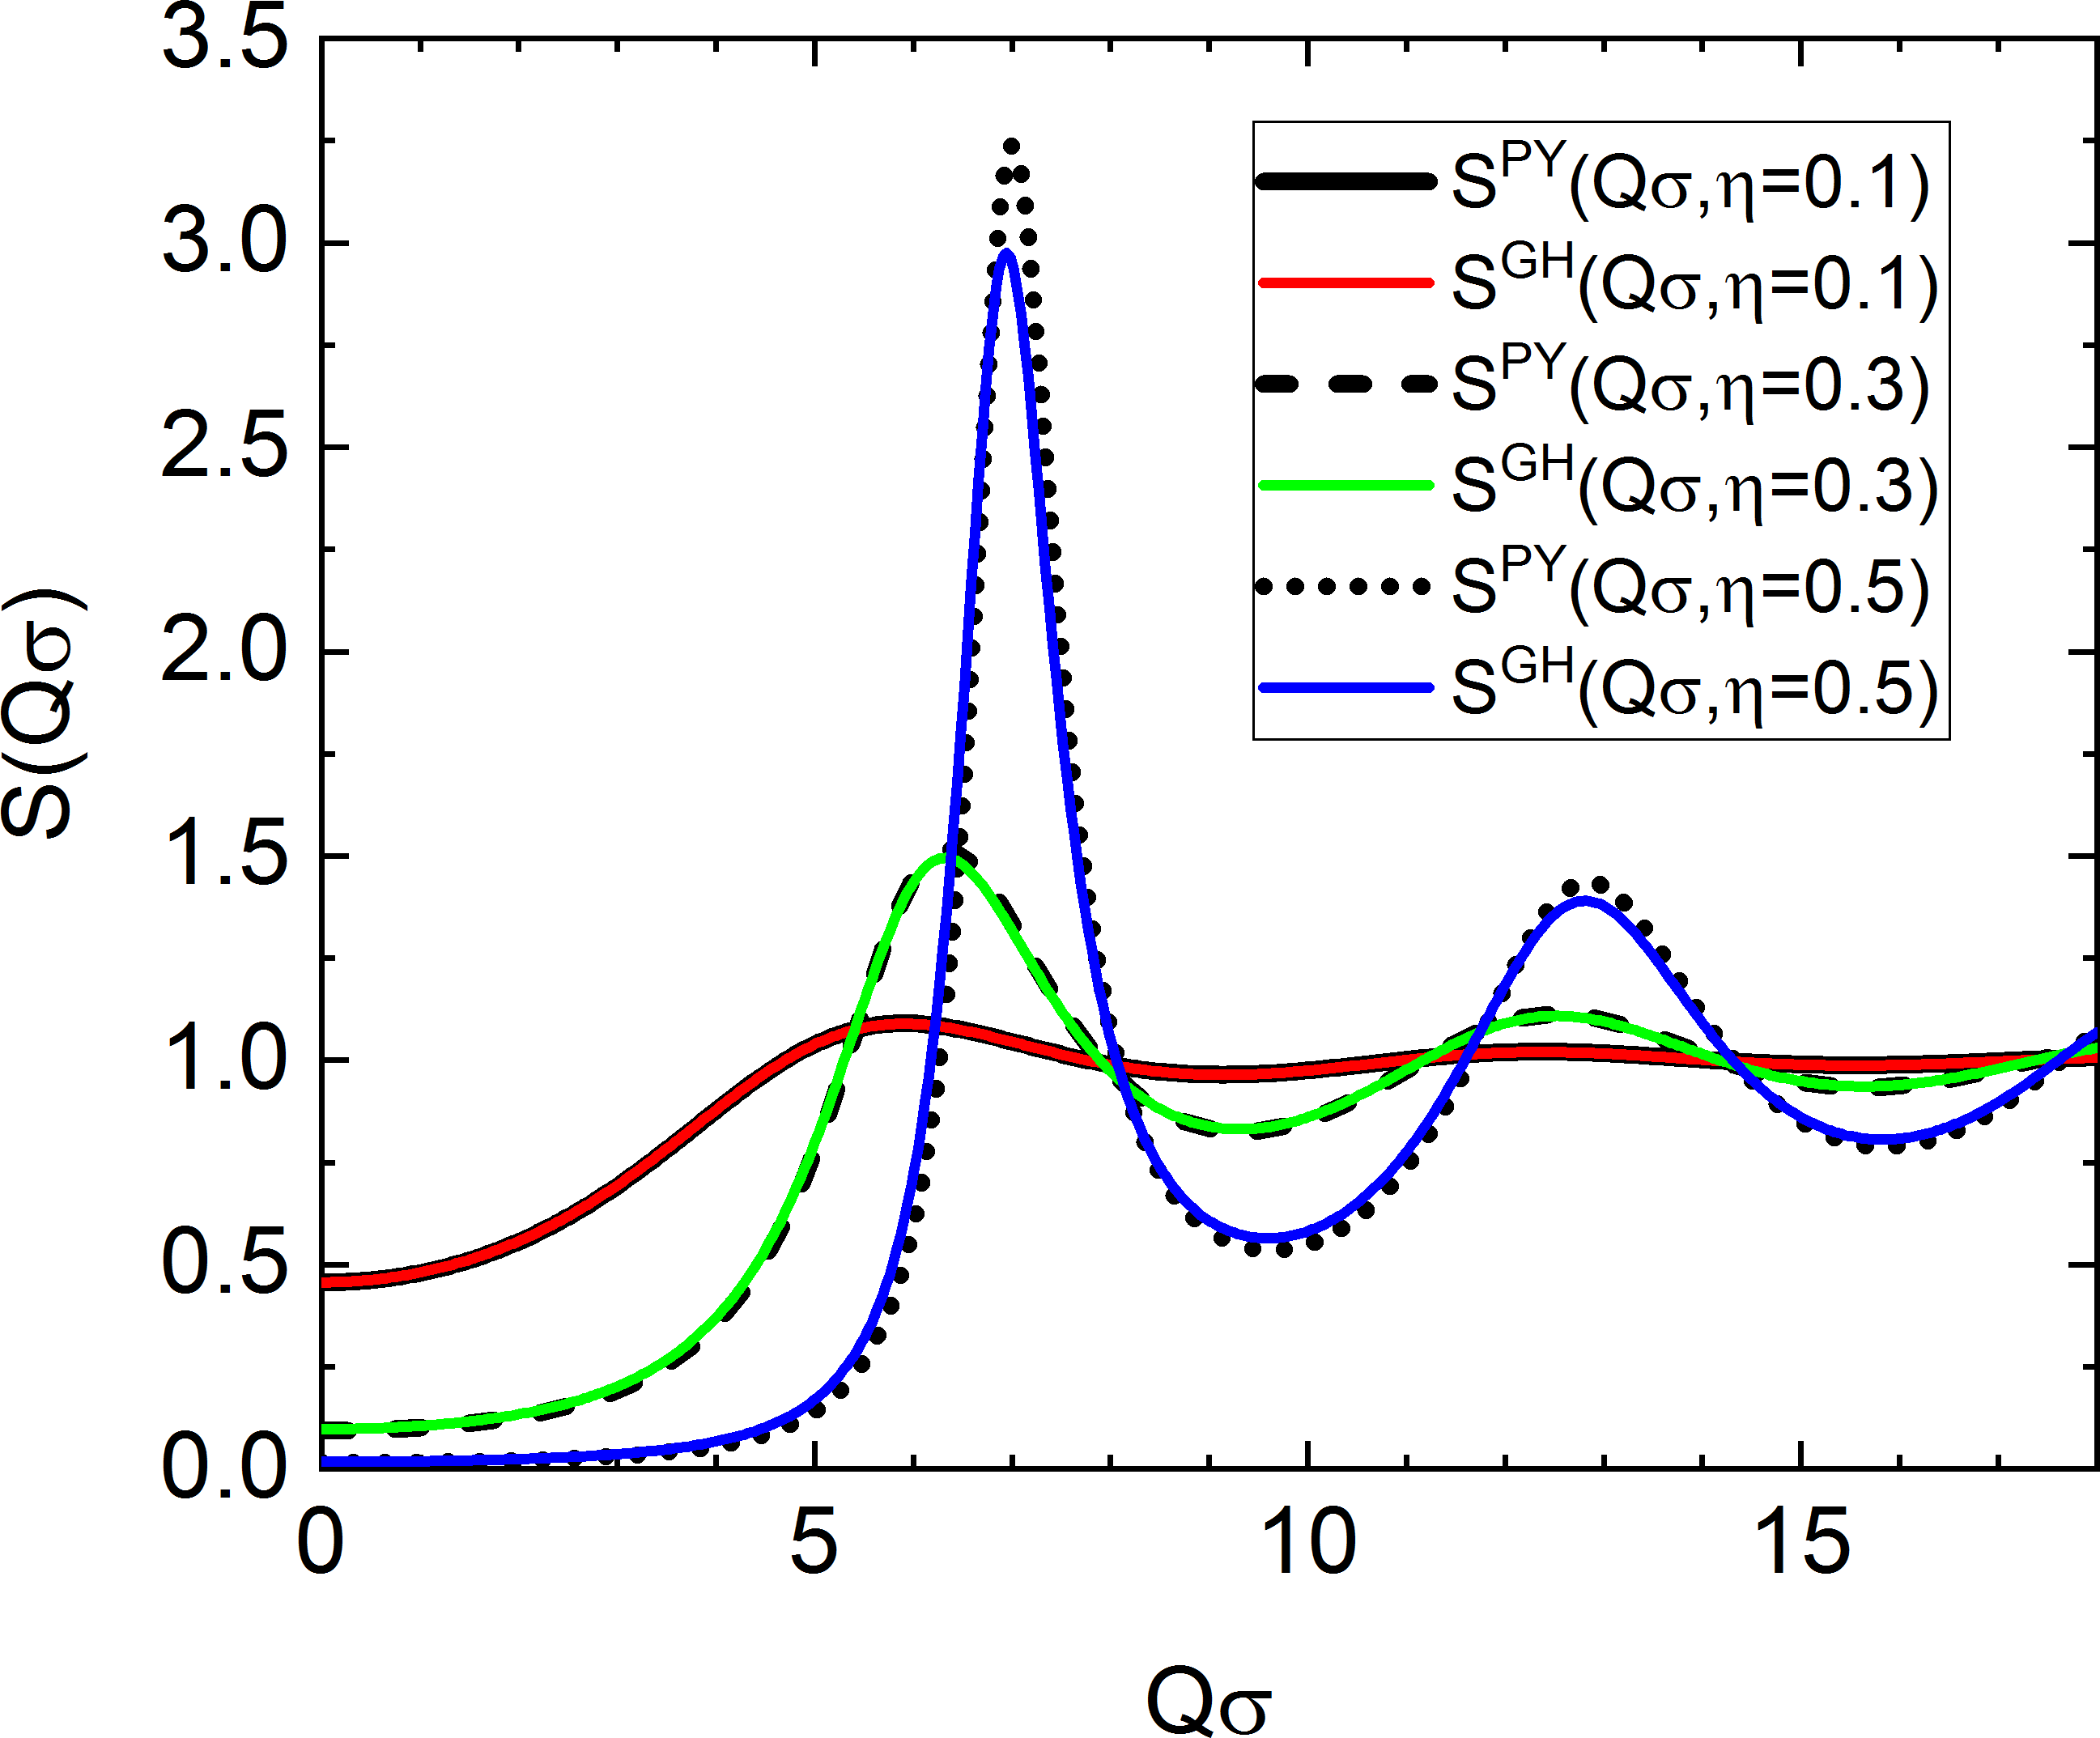
\includegraphics[width=1\textwidth]{../images/structure_factor/HardSphere/SQGH.png}
   \caption{Comparison between $S^\mathrm{PY}$ and $S^\mathrm{GH}$}
   \label{fig:SQ:GH_1}
\end{subfigure}
\hfill
\begin{subfigure}[b]{.48\textwidth}
   \centering
   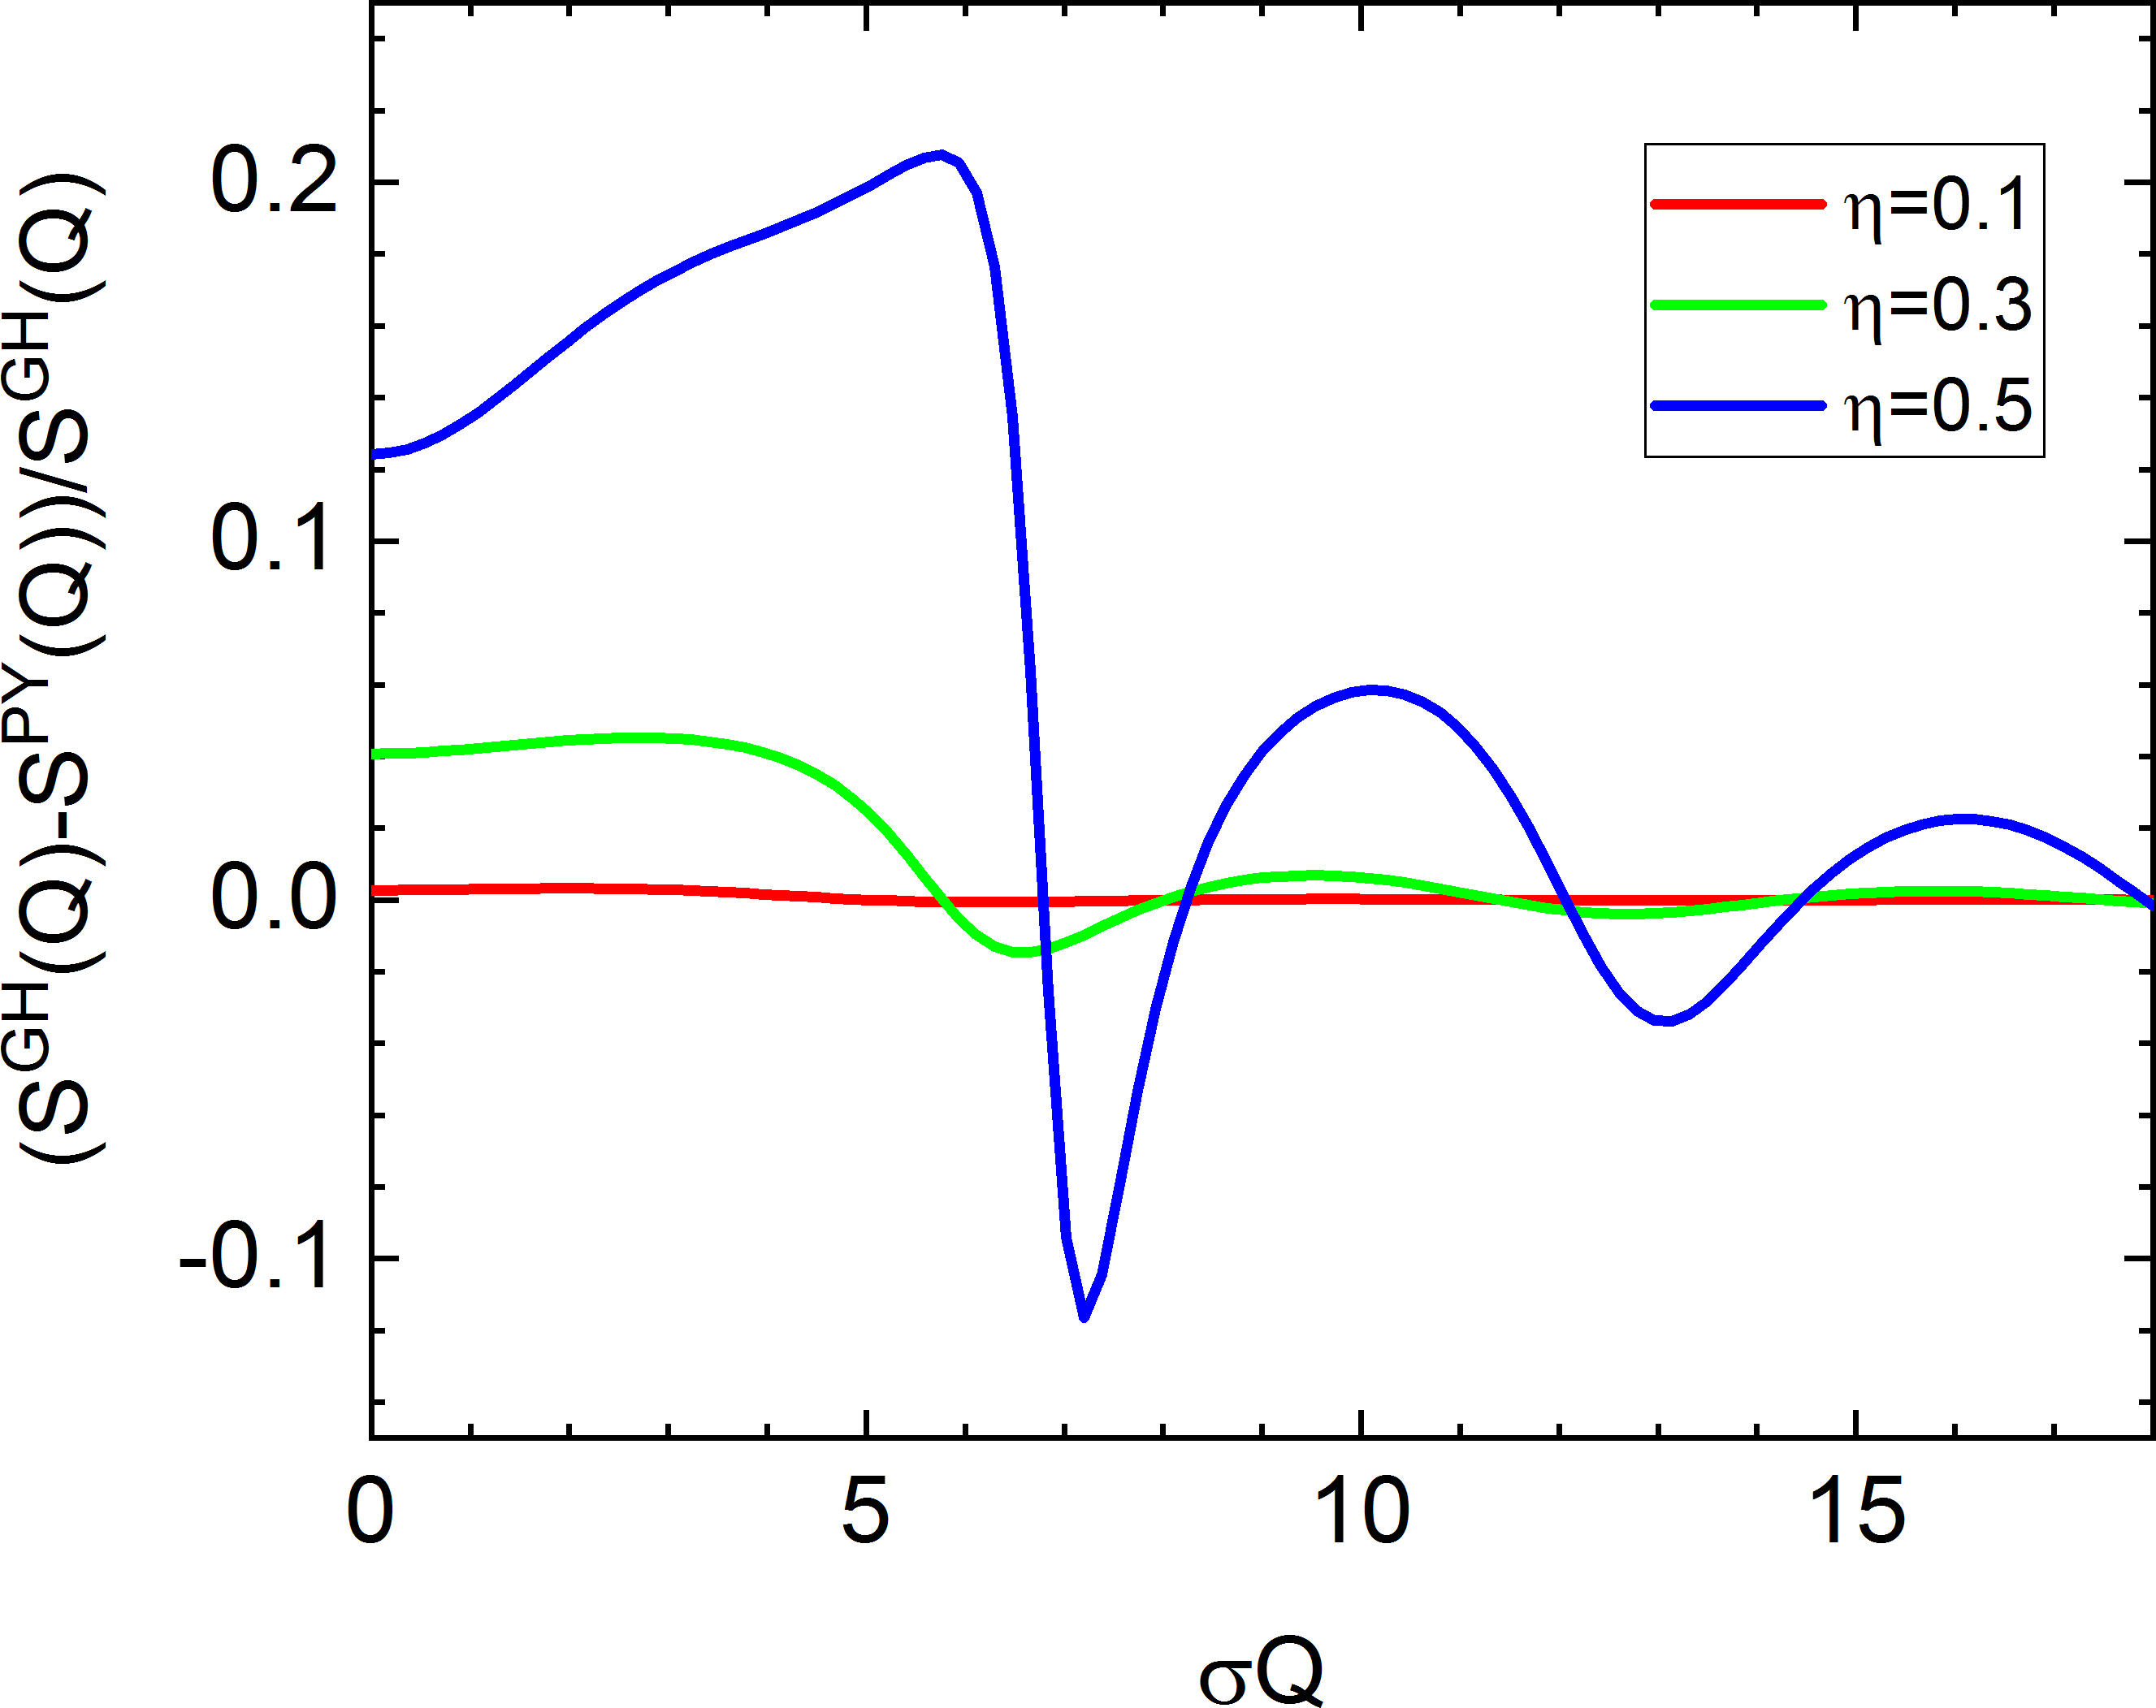
\includegraphics[width=1\textwidth]{../images/structure_factor/HardSphere/ResGH.png}
   \caption{residual between $S^\mathrm{PY}$ and $S^\mathrm{GH}$}
   \label{fig:SQ:GH_2}
\end{subfigure}
\caption{Comparison between analytical PY solution of hard sphere static structure factor and thermodynamically consistent correction as described by Henderson and Grundke}
\label{fig:SQ:GH}
\end{figure}

\clearpage
\subsection{Hard Sphere (PY)} \label{sec:SQ:PY}~\\

\noindent This is the classical analytical solution of the Percus-Yevick equations \cite{Percus1958,Wertheim1963,Vrij1979} for a hard sphere potential
\begin{equation}
U(r) =
 \begin{cases}
      \infty    & \text{for} \quad 0<r<2R \\
      0         & \text{for} \quad r>2R
   \end{cases}
\end{equation}
The structure factor $S^\mathrm{PY}(Q)$ can be calculated
\begin{subequations}
\begin{align}
\alpha &= \frac{\left(1+2\eta\right)^2}{\left(1-\eta\right)^4} \\
\beta  &= -6 \eta \frac{\left(1 +\eta/2 \right)^2}{\left(1-\eta\right)^4} \\
\gamma &= \frac{\eta \alpha}{2}  \\
A &= 2 R Q
\end{align}

\begin{align}
G(\eta,A) =  & \, \alpha \, \frac{\sin A -A \cos A }{A^2} + \beta \, \frac{2 A \sin A +(2-A^2) \cos A -2}{A^3} + \nonumber \\
    & \, \gamma  \, \frac{-A^4 \cos A + 4\left[(3A^2-6)\cos A+(A^3-6A)\sin A+6\right]}{A^5}
\end{align}
\begin{align}
S^\mathrm{PY}(Q,R,\eta)  = & \cfrac{1}{1+24 \eta
\cfrac{G(\eta,A)}{A}}
\end{align}
\end{subequations}

\vspace{5mm}

\hspace{1pt}\\
\uline{Input parameters for \texttt{3D Hard Sphere (PY)}:}
\begin{description}
    \item[\texttt{R}]  radius $R$
    \item[\texttt{eta}] volume fraction $\eta$
\end{description}

\noindent
\uline{Note}
\begin{itemize}
\item The structure factor accepts volume fractions between $\eta \in [0,1]$.
\end{itemize}

\begin{figure}[htb]
\begin{center}
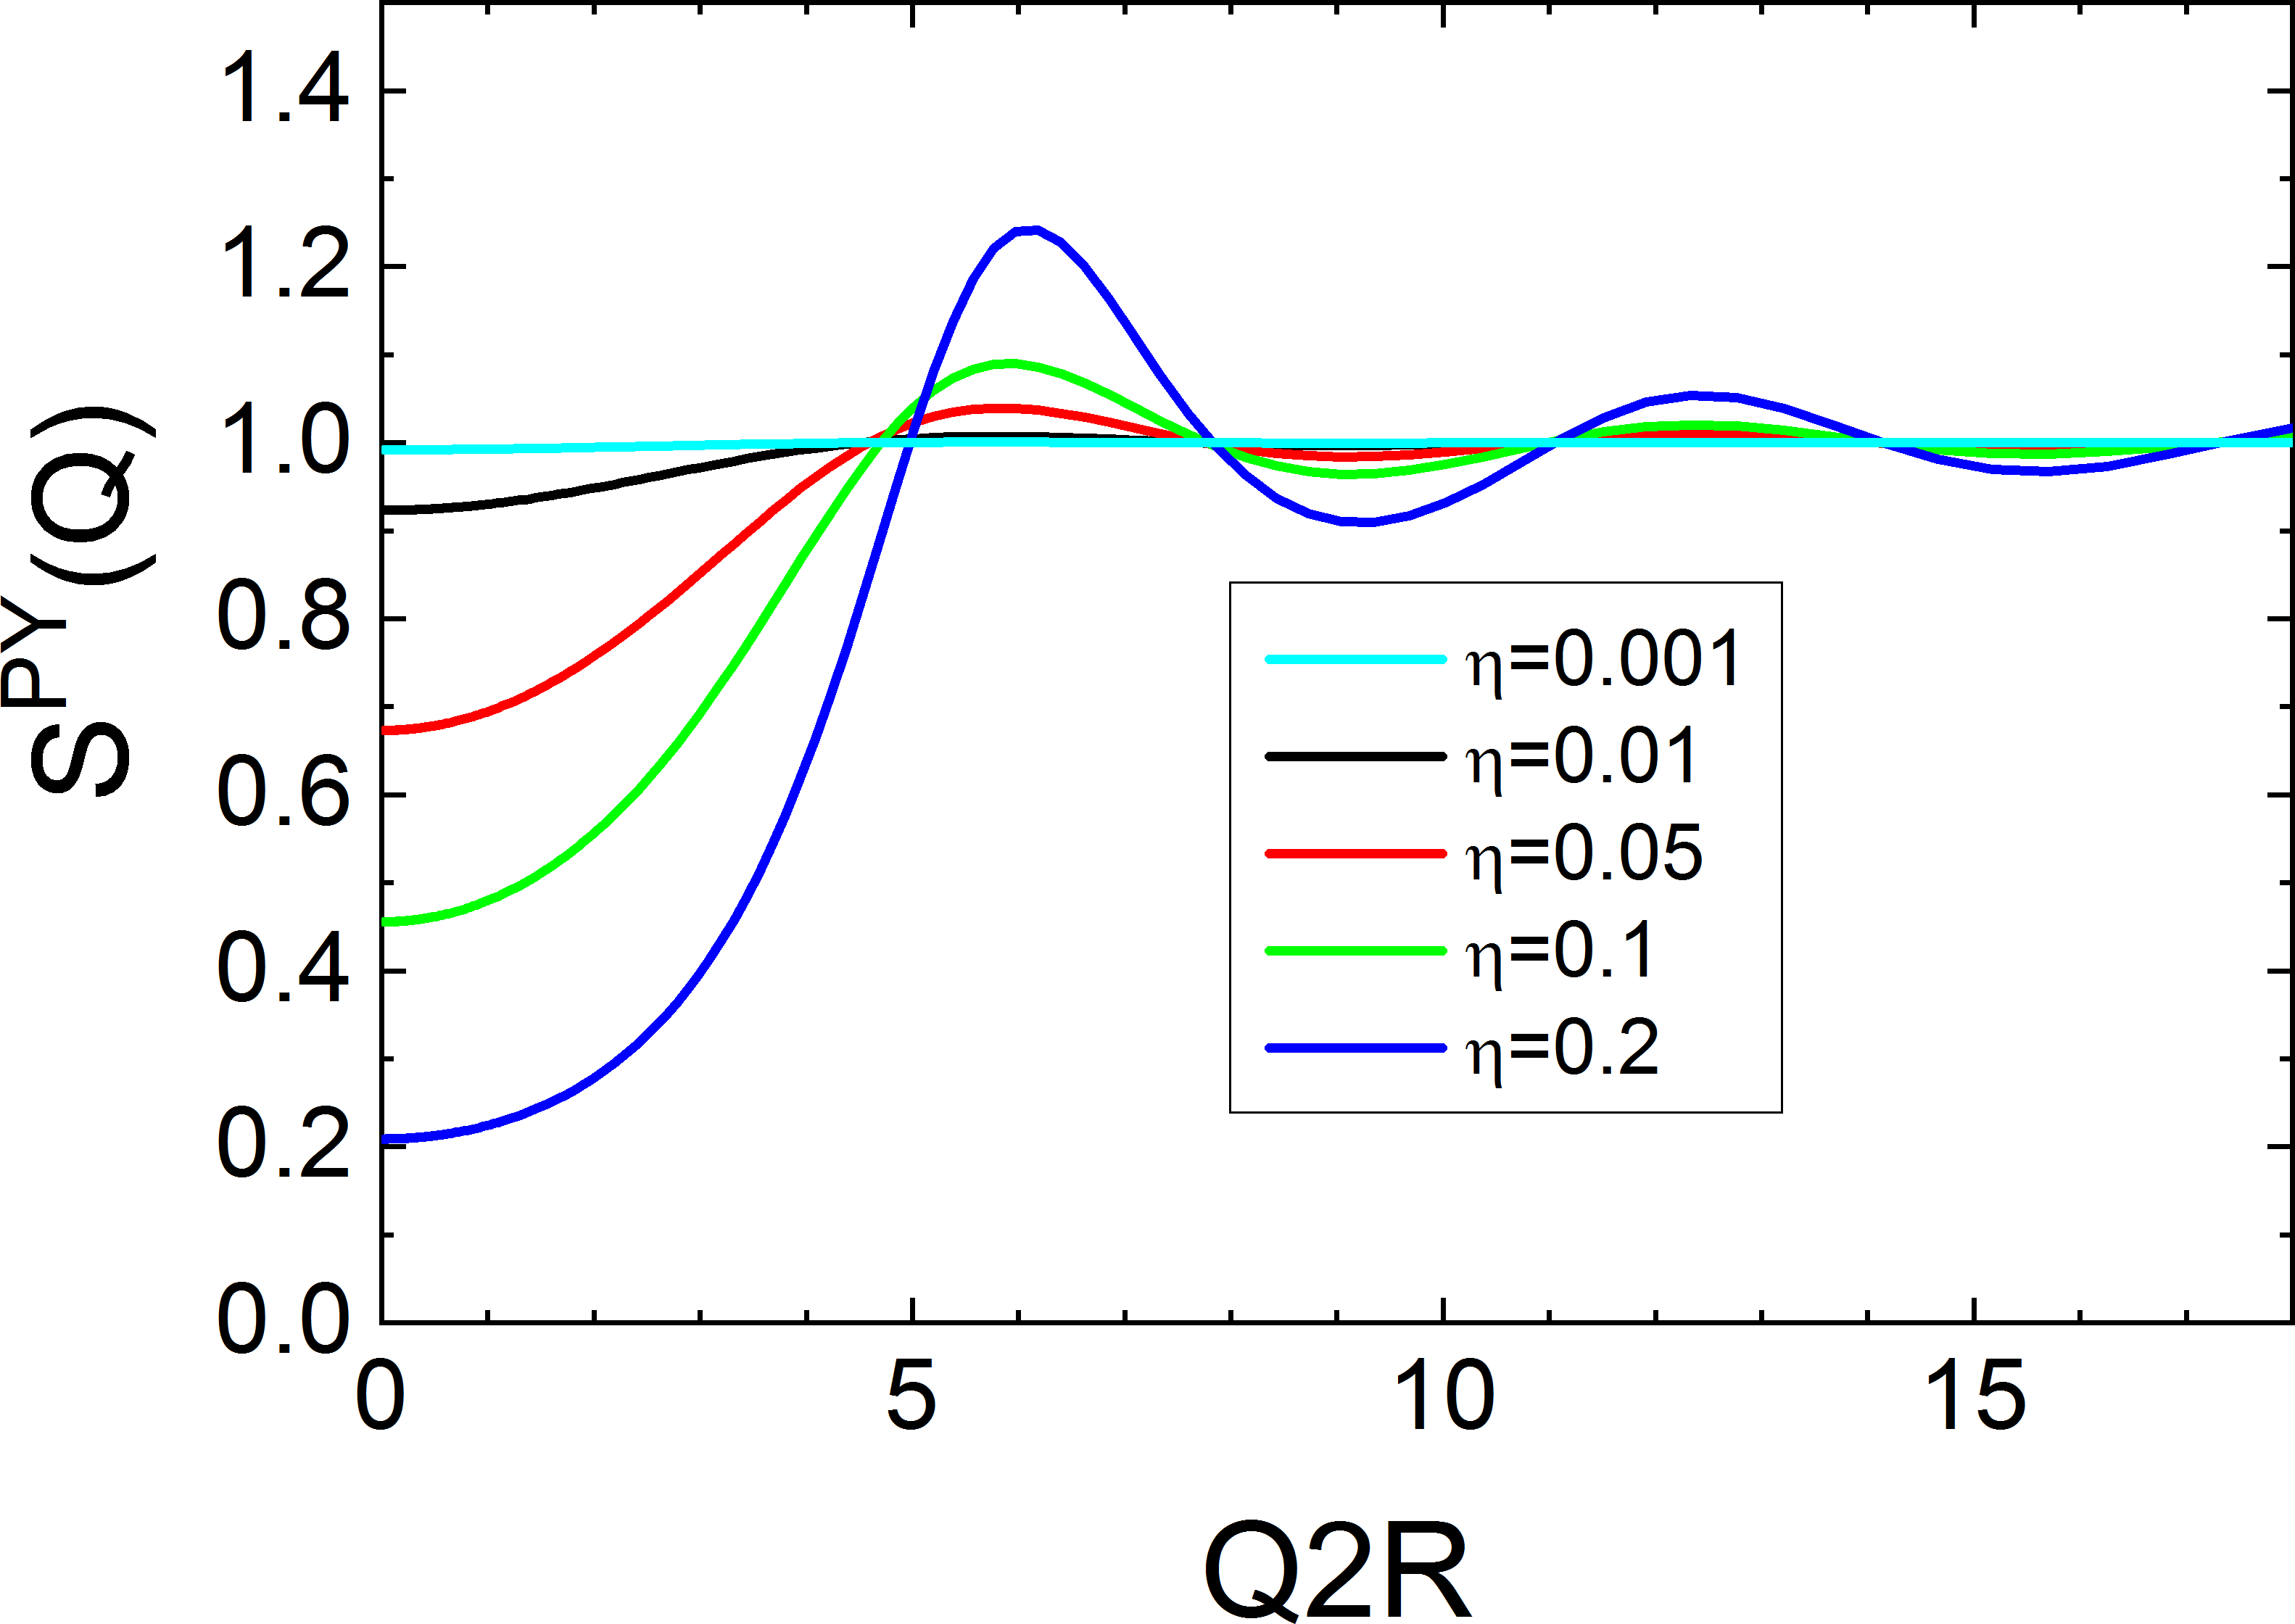
\includegraphics[width=0.6\textwidth]{../images/structure_factor/HardSphere/SQPY.png}
\end{center}
\caption{Structure factor $S^\mathrm{PY}(Q)$ for a hard sphere interaction potential for the different volume fractions $\eta$.}
\label{fig:SQPYHardSphere}
\end{figure}

\clearpage
\section{Structure factor for a two dimensional hard spheres/disks fluid} \hspace{1pt}
The structure factor of hard disks or spheres with diameter/radius $\sigma=2R$ in two dimensions with an interaction potential
\begin{align}
U(r,\sigma) &=
\begin{cases}
\infty &\mathrm{for~}  r < \sigma \\
0  &\mathrm{for~}  r \geq \sigma
\end{cases}
\end{align}
have been implemented in several variants. All the theories are developed for $\mathbf{q}$-vector in the plane of the two dimensional structure. However, in an experiment this plane might be tilted against the detection plane. Therefore
in all cases two variants are implemented. One case is considering a certain direction of the normal of the two dimensional sample plane and a second one for a randomly oriented plane, i.e. the limit of a powder.
The coordination system used to describe the normal of the 2D plane is defined in fig.\ \ref{fig:coord_SQ2D}.
\begin{figure}[htb]
\begin{center}
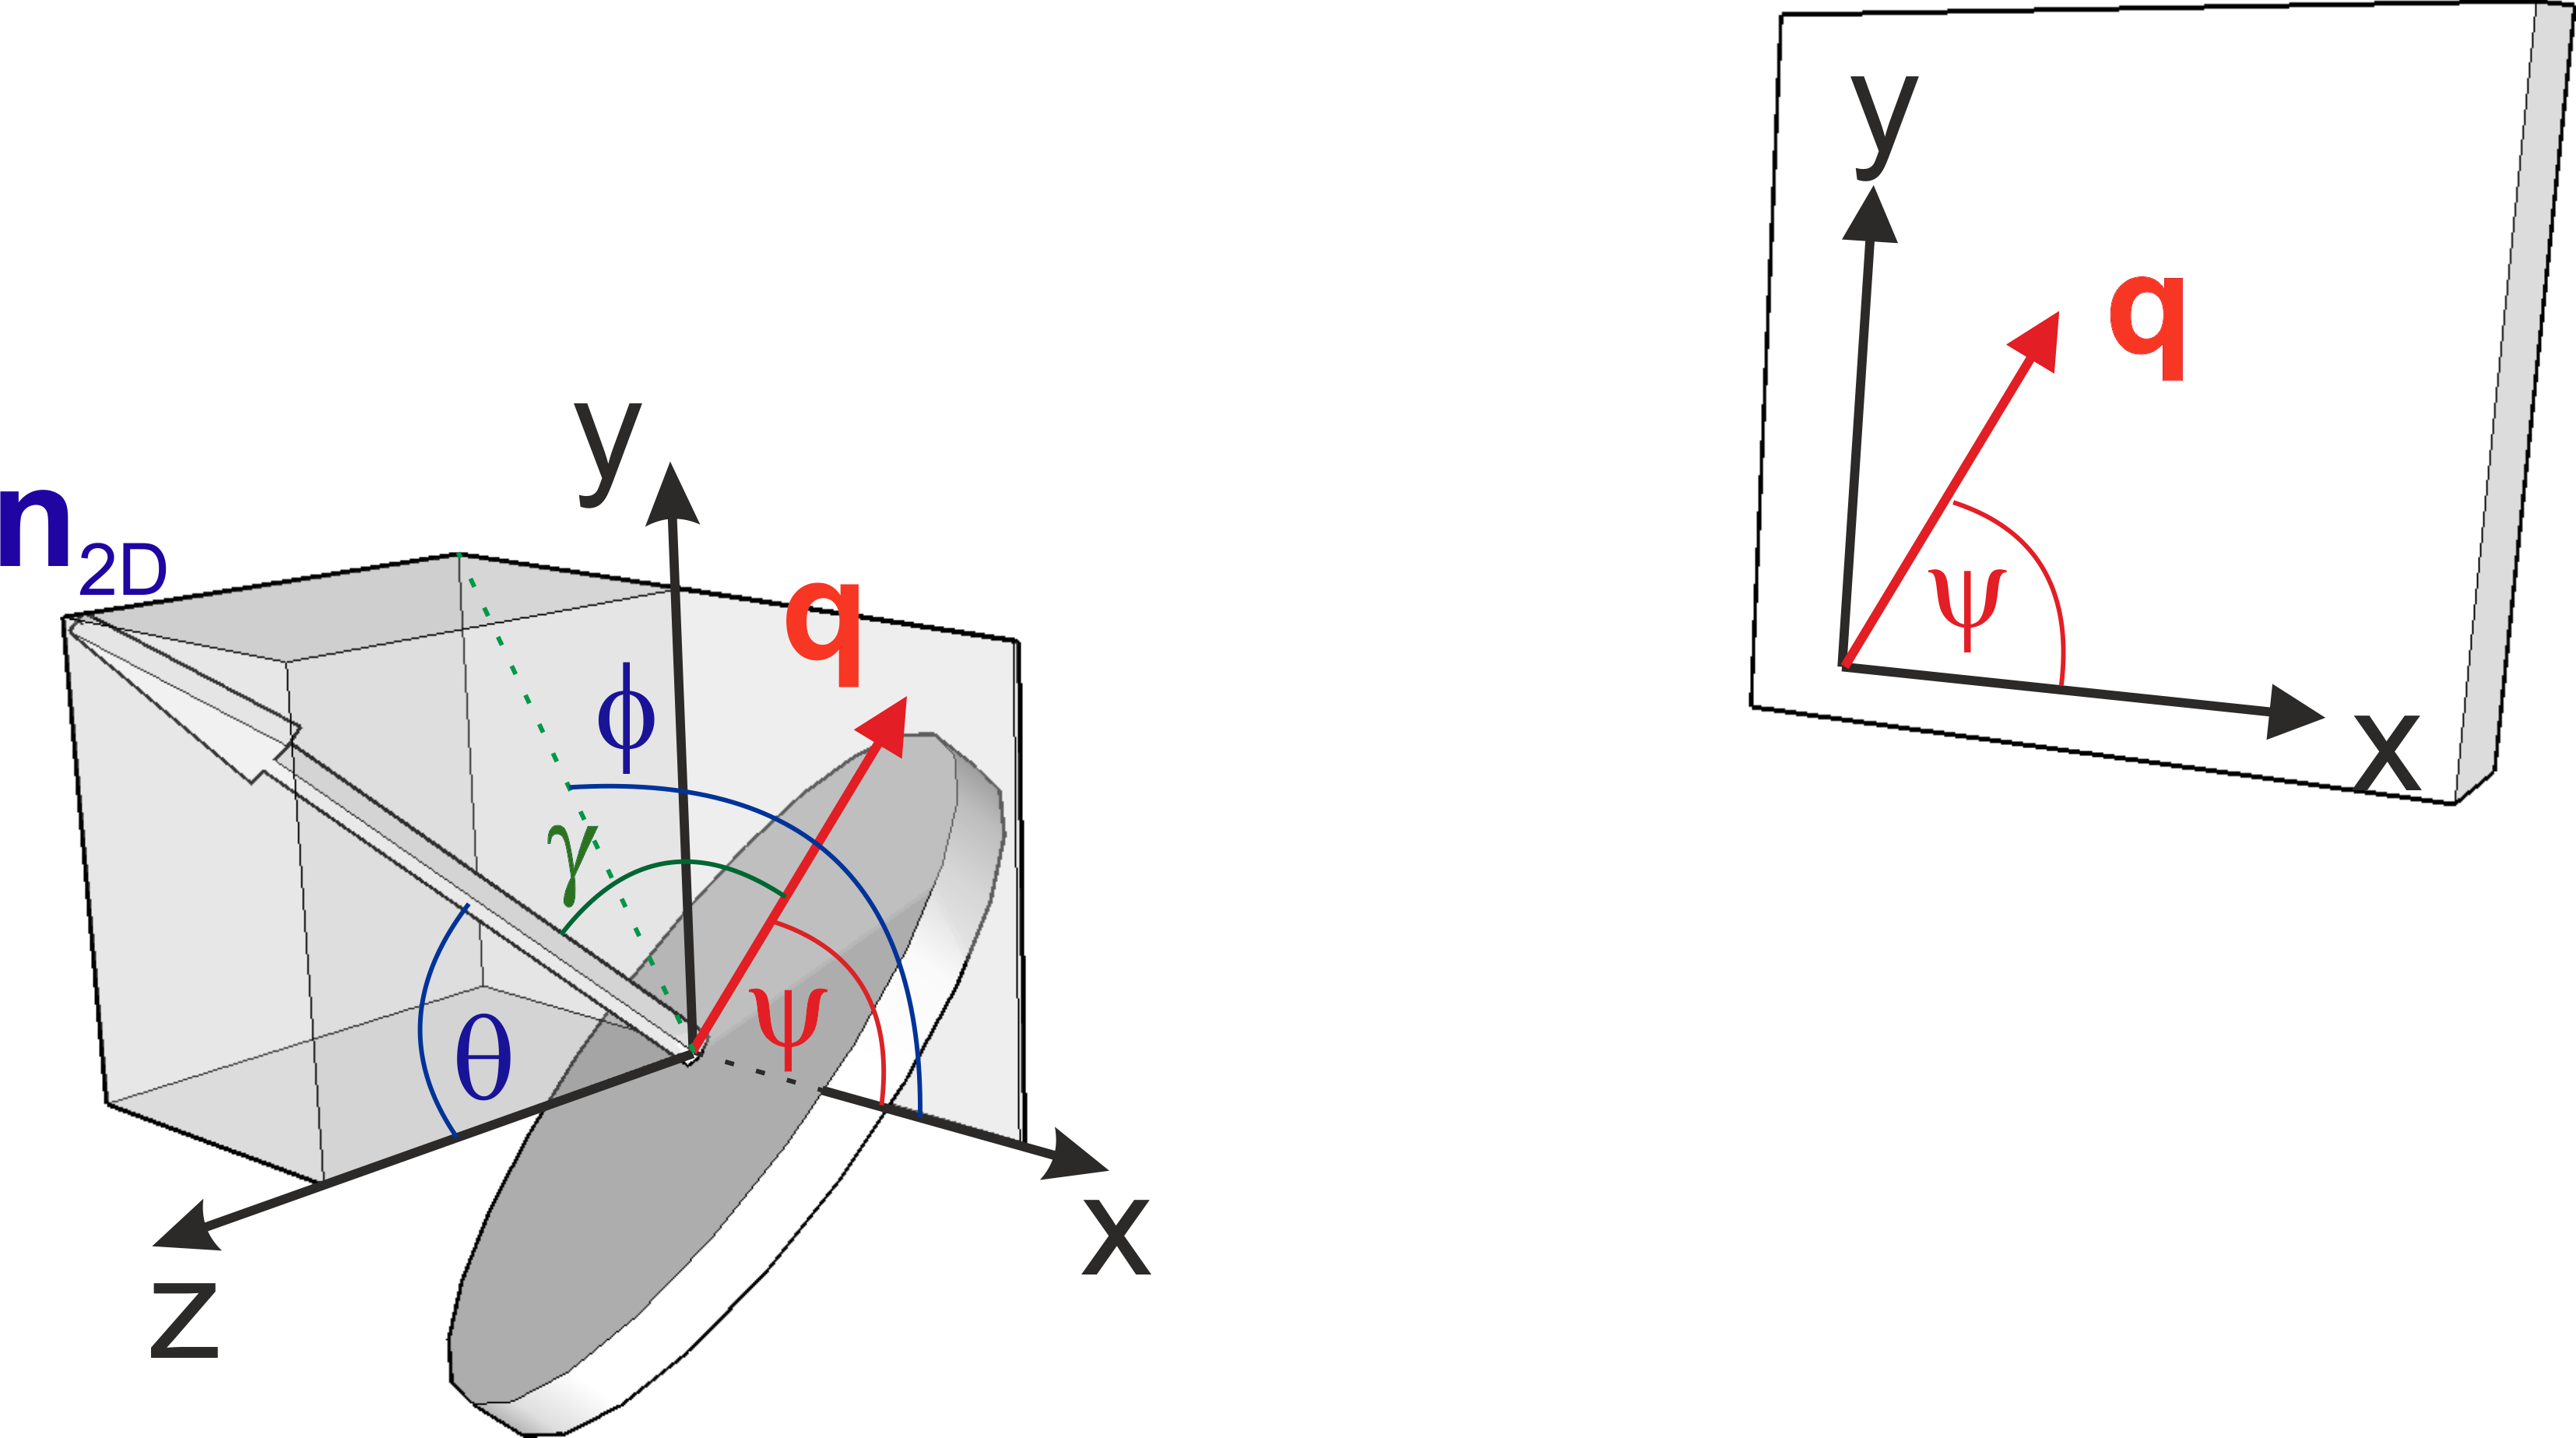
\includegraphics[width=0.75\textwidth]{../images/structure_factor/SQ_1D_2D/coord_SQ_2D.png}
\end{center}
\caption{coordination system for 2D structure factors relative to the beam direction.}
\label{fig:coord_SQ2D}
\end{figure}
With the following definition for the scattering vector and the unit vector defining the direction of the 1D structure
\begin{align}
  \mathbf{q} &=q  \begin{pmatrix}
               \cos \psi \\
               \sin psi \\
               0 \\
             \end{pmatrix}
   \mbox{~~and~~}
  \mathbf{n}_\mathrm{2D} =
    \begin{pmatrix}
        \sin \theta \cos \phi  \\
        \sin \theta \sin \phi \\
        \cos \theta \\
    \end{pmatrix} \\
\end{align}
the angle $\gamma$ between $\mathbf{q}$ and $ \mathbf{n}_\mathrm{2D}$ is given as
\begin{align}
  \cos\gamma &= \cos\psi\sin\theta\cos\phi+\sin\psi\sin\theta\sin\phi
\end{align}
\subsection{Two dimensional hard sphere/disks fluid according to Rosenfeld}
~\\

An analytical form of the structure factor as a function of the disk radius $R$ and surface coverage $\eta=\pi R^2 \rho$, where $\rho$ is the number density of particles, have been given by\cite{Rosenfeld1990,Guo2006}.
Rosenfeld \cite{Rosenfeld1990} gives the expression
\begin{align}
\begin{split}
\frac{1}{S_\mathrm{Rosenfeld}(q\sin\gamma)}-1 = &
4\eta
                    \left(A \frac{\mathrm{J}_1^2(qR\sin\gamma)}{(qR\sin\gamma)^2} \right) \\
                   & +B\mathrm{J}_0(qR\sin\gamma)\frac{\mathrm{J}_1(qR\sin\gamma)}{qR\sin\gamma} \left. +G\frac{\mathrm{J}_1(2qR\sin\gamma)}{qR\sin\gamma}  \right)
\end{split}
\end{align}
with
\begin{align}
A &=\left(1+(2\eta-1)\chi+2\eta G\right)/\eta \\
B &=\left((1-\eta)\chi-1-3\eta G\right)/\eta \\
G &= \frac{1}{1-\eta} \\
\chi &= \frac{1+\eta}{(1-\eta)^2}
\end{align}
In the original paper from Rosenfeld the definition of $\chi$ seems to have a typo and has been corrected like in \cite{Engel2009}.

\subsection {Two dimensional hard sphere/disks fluid according to Guo}
~\\

Guo \cite{Guo2006} supplies the expression
\begin{align}
S_\mathrm{Guo}(q\sin\gamma) &= \frac{1}{1-\rho \tilde{c}(q\sin\gamma,r)} \\
\tilde{c}(q\sin\gamma,r) &= 2\pi\sigma^2 \int_0^1 c(r',\eta) J_0(q\sin\gamma\sigma r') r' \mathrm{d}r'
\end{align}
with
\begin{align}
\begin{split}
c(r',\eta) &=
\Theta(1-r') \left[-\frac{1-p\eta^2}{\left(1-2\eta+p\eta^2\right)^2}\right]  \\
&\left\{1-a^2\eta-a^2\eta\frac{2}{\pi}\left[\arccos\left(\frac{r'}{a}\right)-\frac{r'}{a}\sqrt{1-\frac{r'^2}{a^2}}\right]\right\}
\end{split}
\end{align}
with $p=\left(4\sqrt{3}\pi-12\right)/\pi^2$ and $\Theta()$ being the Heaviside function. The parameter $a$ is the root of a non-linear equation, which has been solved numerically and then approximated via a polynomial fitting by
\begin{align}
a &= 0.3699\eta^4
      -1.2511\eta^3
      +2.0199\eta^2
      -2.2373\eta
      +2.1
\end{align}

\vspace{5mm}
\noindent
\uline{Input Parameters for model \texttt{2D hard disks (Rosenfeld,aligned)} as well as}
\uline{\texttt{2D hard disks (Guo,aligned)}:}\\
\begin{description}
\item[\texttt{R}] radius of the disc $R$
\item[\texttt{eta}] surface coverage $\eta$
\item[\texttt{theta}] polar angle $\theta$ (polar axis = beam axis)
\item[\texttt{phi}] azimuthal angle $\phi$ (in detector plane towards $x$-axis)
\item[\texttt{psi}] azimuthal angle  $\psi$ for $q$ towards $x$-axis
\end{description}

\vspace{5mm}
\noindent
\uline{Input Parameters for model \texttt{2D hard disks (Rosenfeld,random)} as well as}
\uline{\texttt{2D hard disks (Guo,random)}:}\\
\begin{description}
\item[\texttt{R}] radius of the disc $R$
\item[\texttt{eta}] surface coverage $\eta$
\end{description}

\noindent\uline{Note:}
\begin{itemize}
\item Both models break down for surface coverage around $\eta>0.75$. The densest possible lattice packing would be $\eta_\mathrm{max}=\frac16\pi\sqrt{3}\simeq 0.907$.
\item Values for surface coverage $0 < \eta < 1$ are accepted by the software.
\end{itemize}

\begin{figure}[htb]
\begin{subfigure}[b]{.43\textwidth}
   \centering
   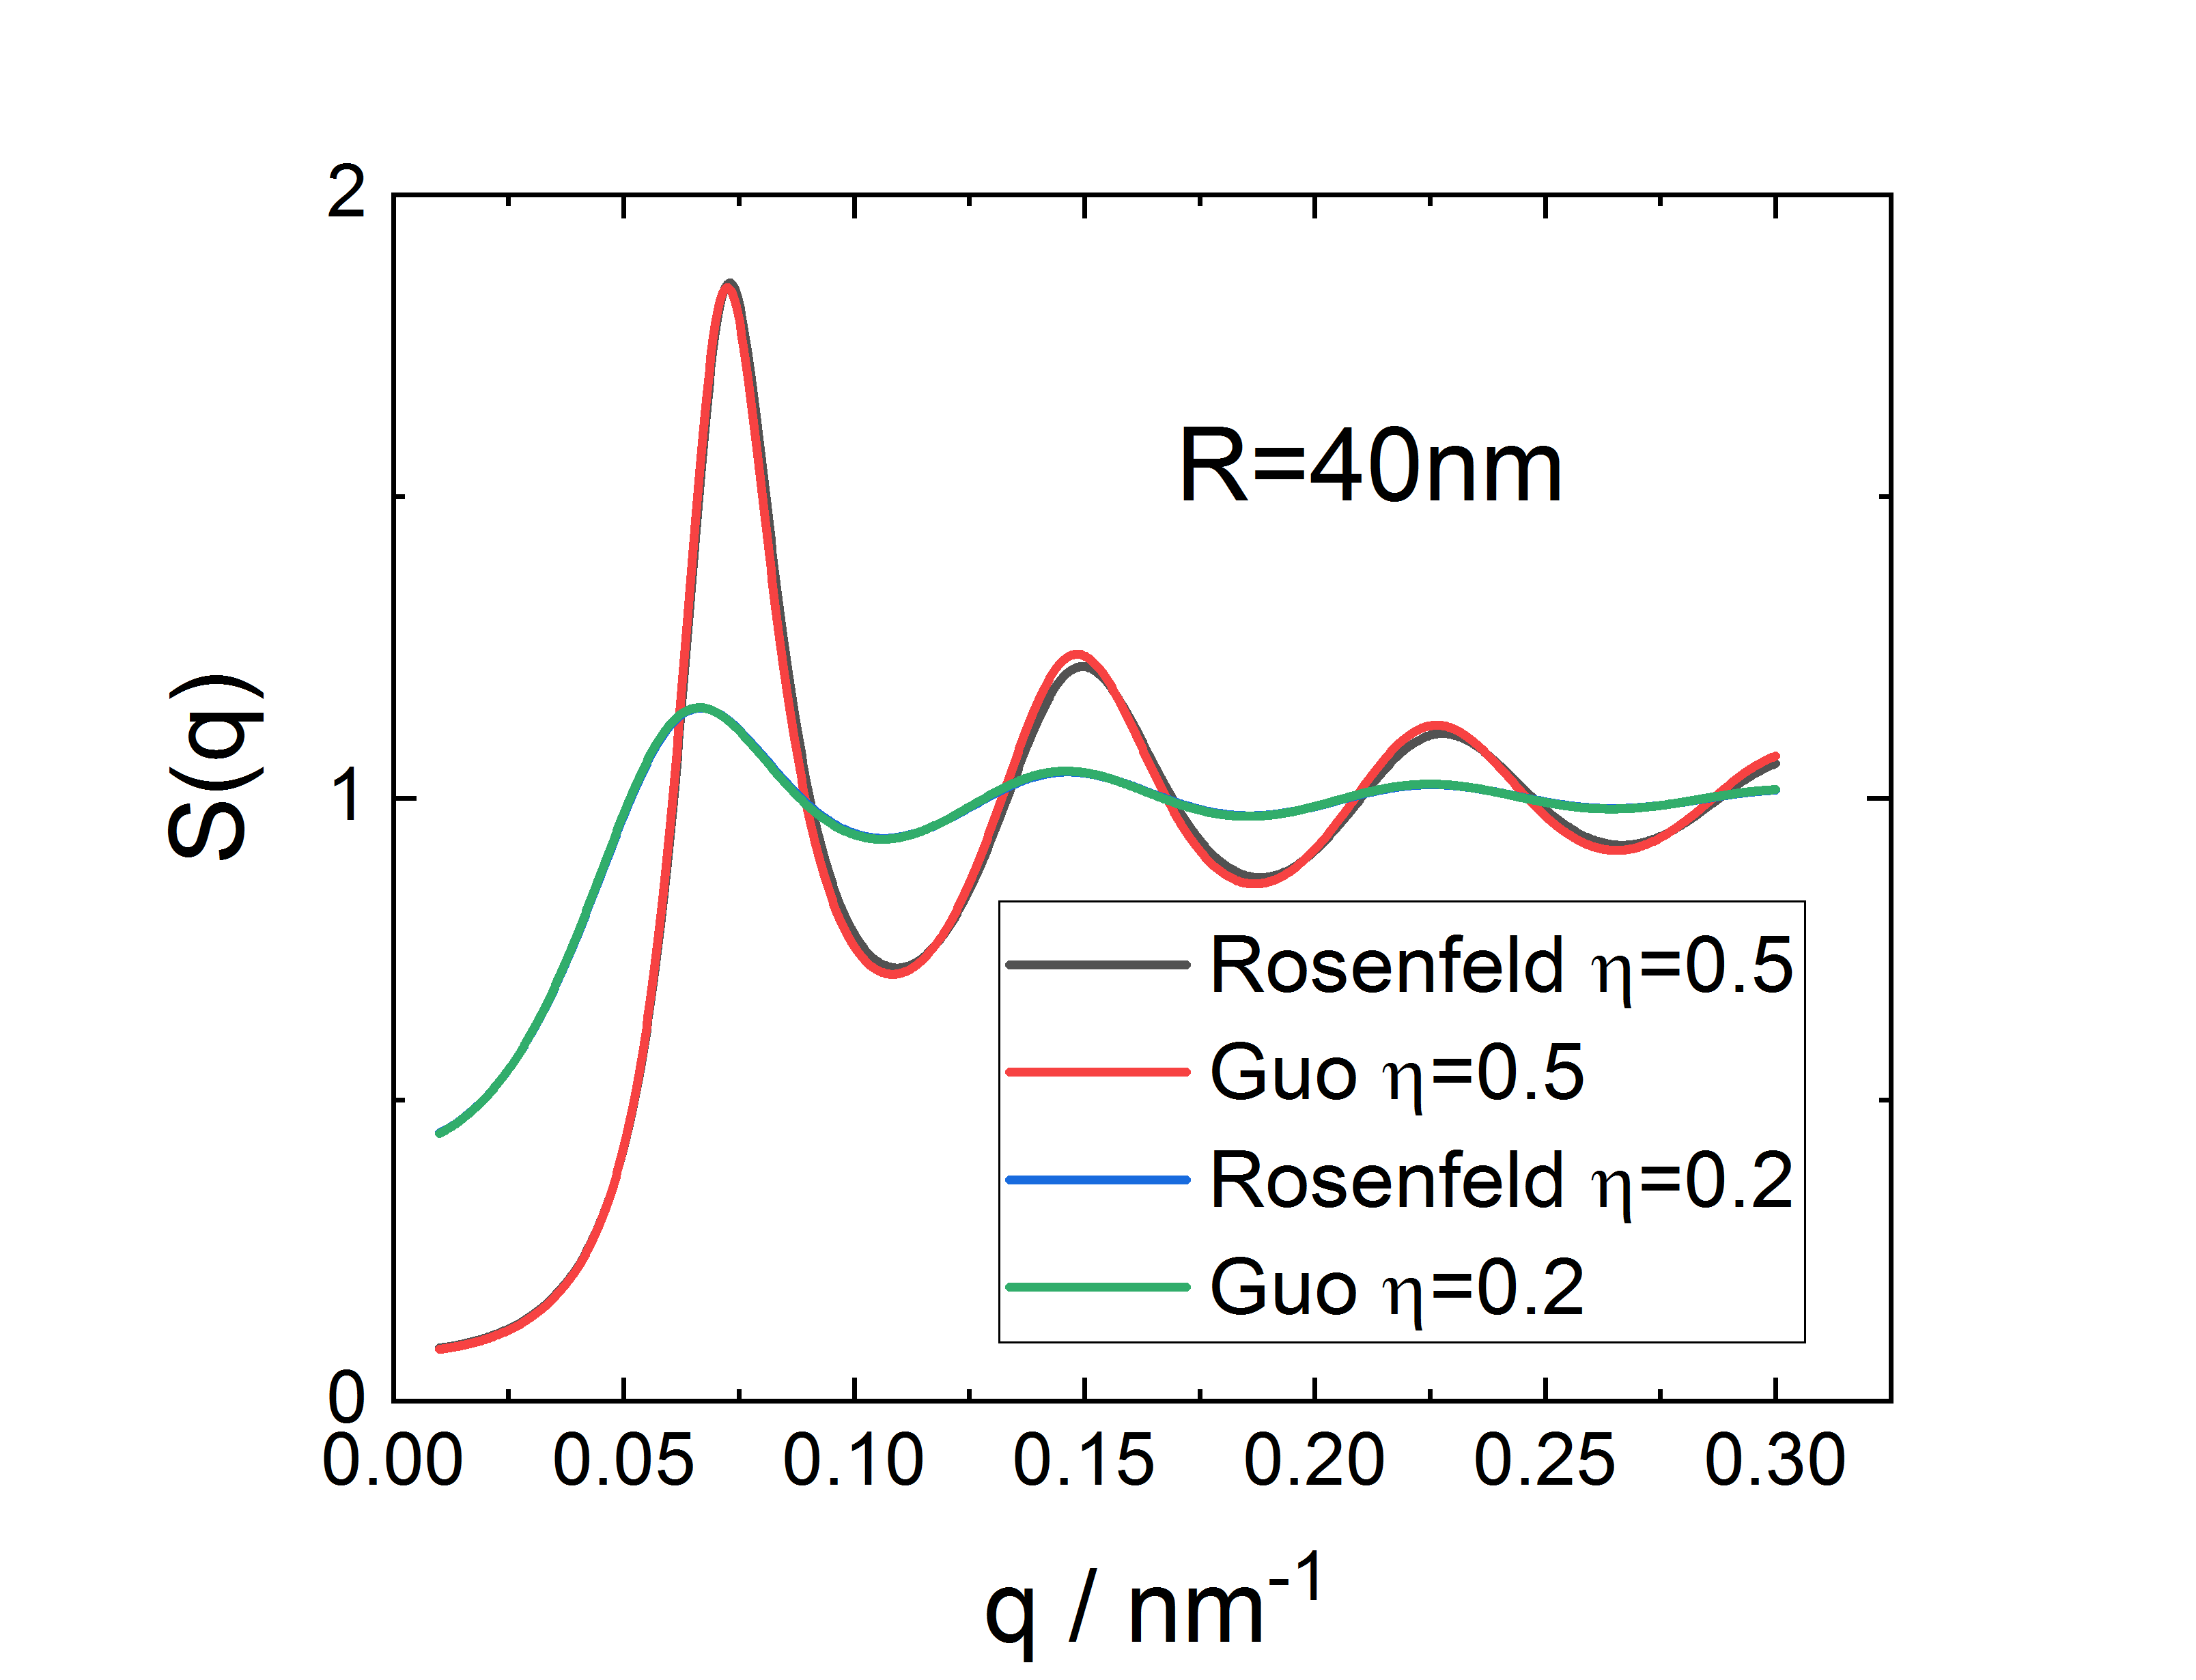
\includegraphics[width=1\textwidth]{../images/structure_factor/2D_hard_disk_fluid/HardDisks_low.png}
   \caption{surface coverage of $\eta=0.2$ and 0.5}
   \label{fig:RosenfeldGuo1}
\end{subfigure}
\hfill
\begin{subfigure}[b]{.47\textwidth}
   \centering
   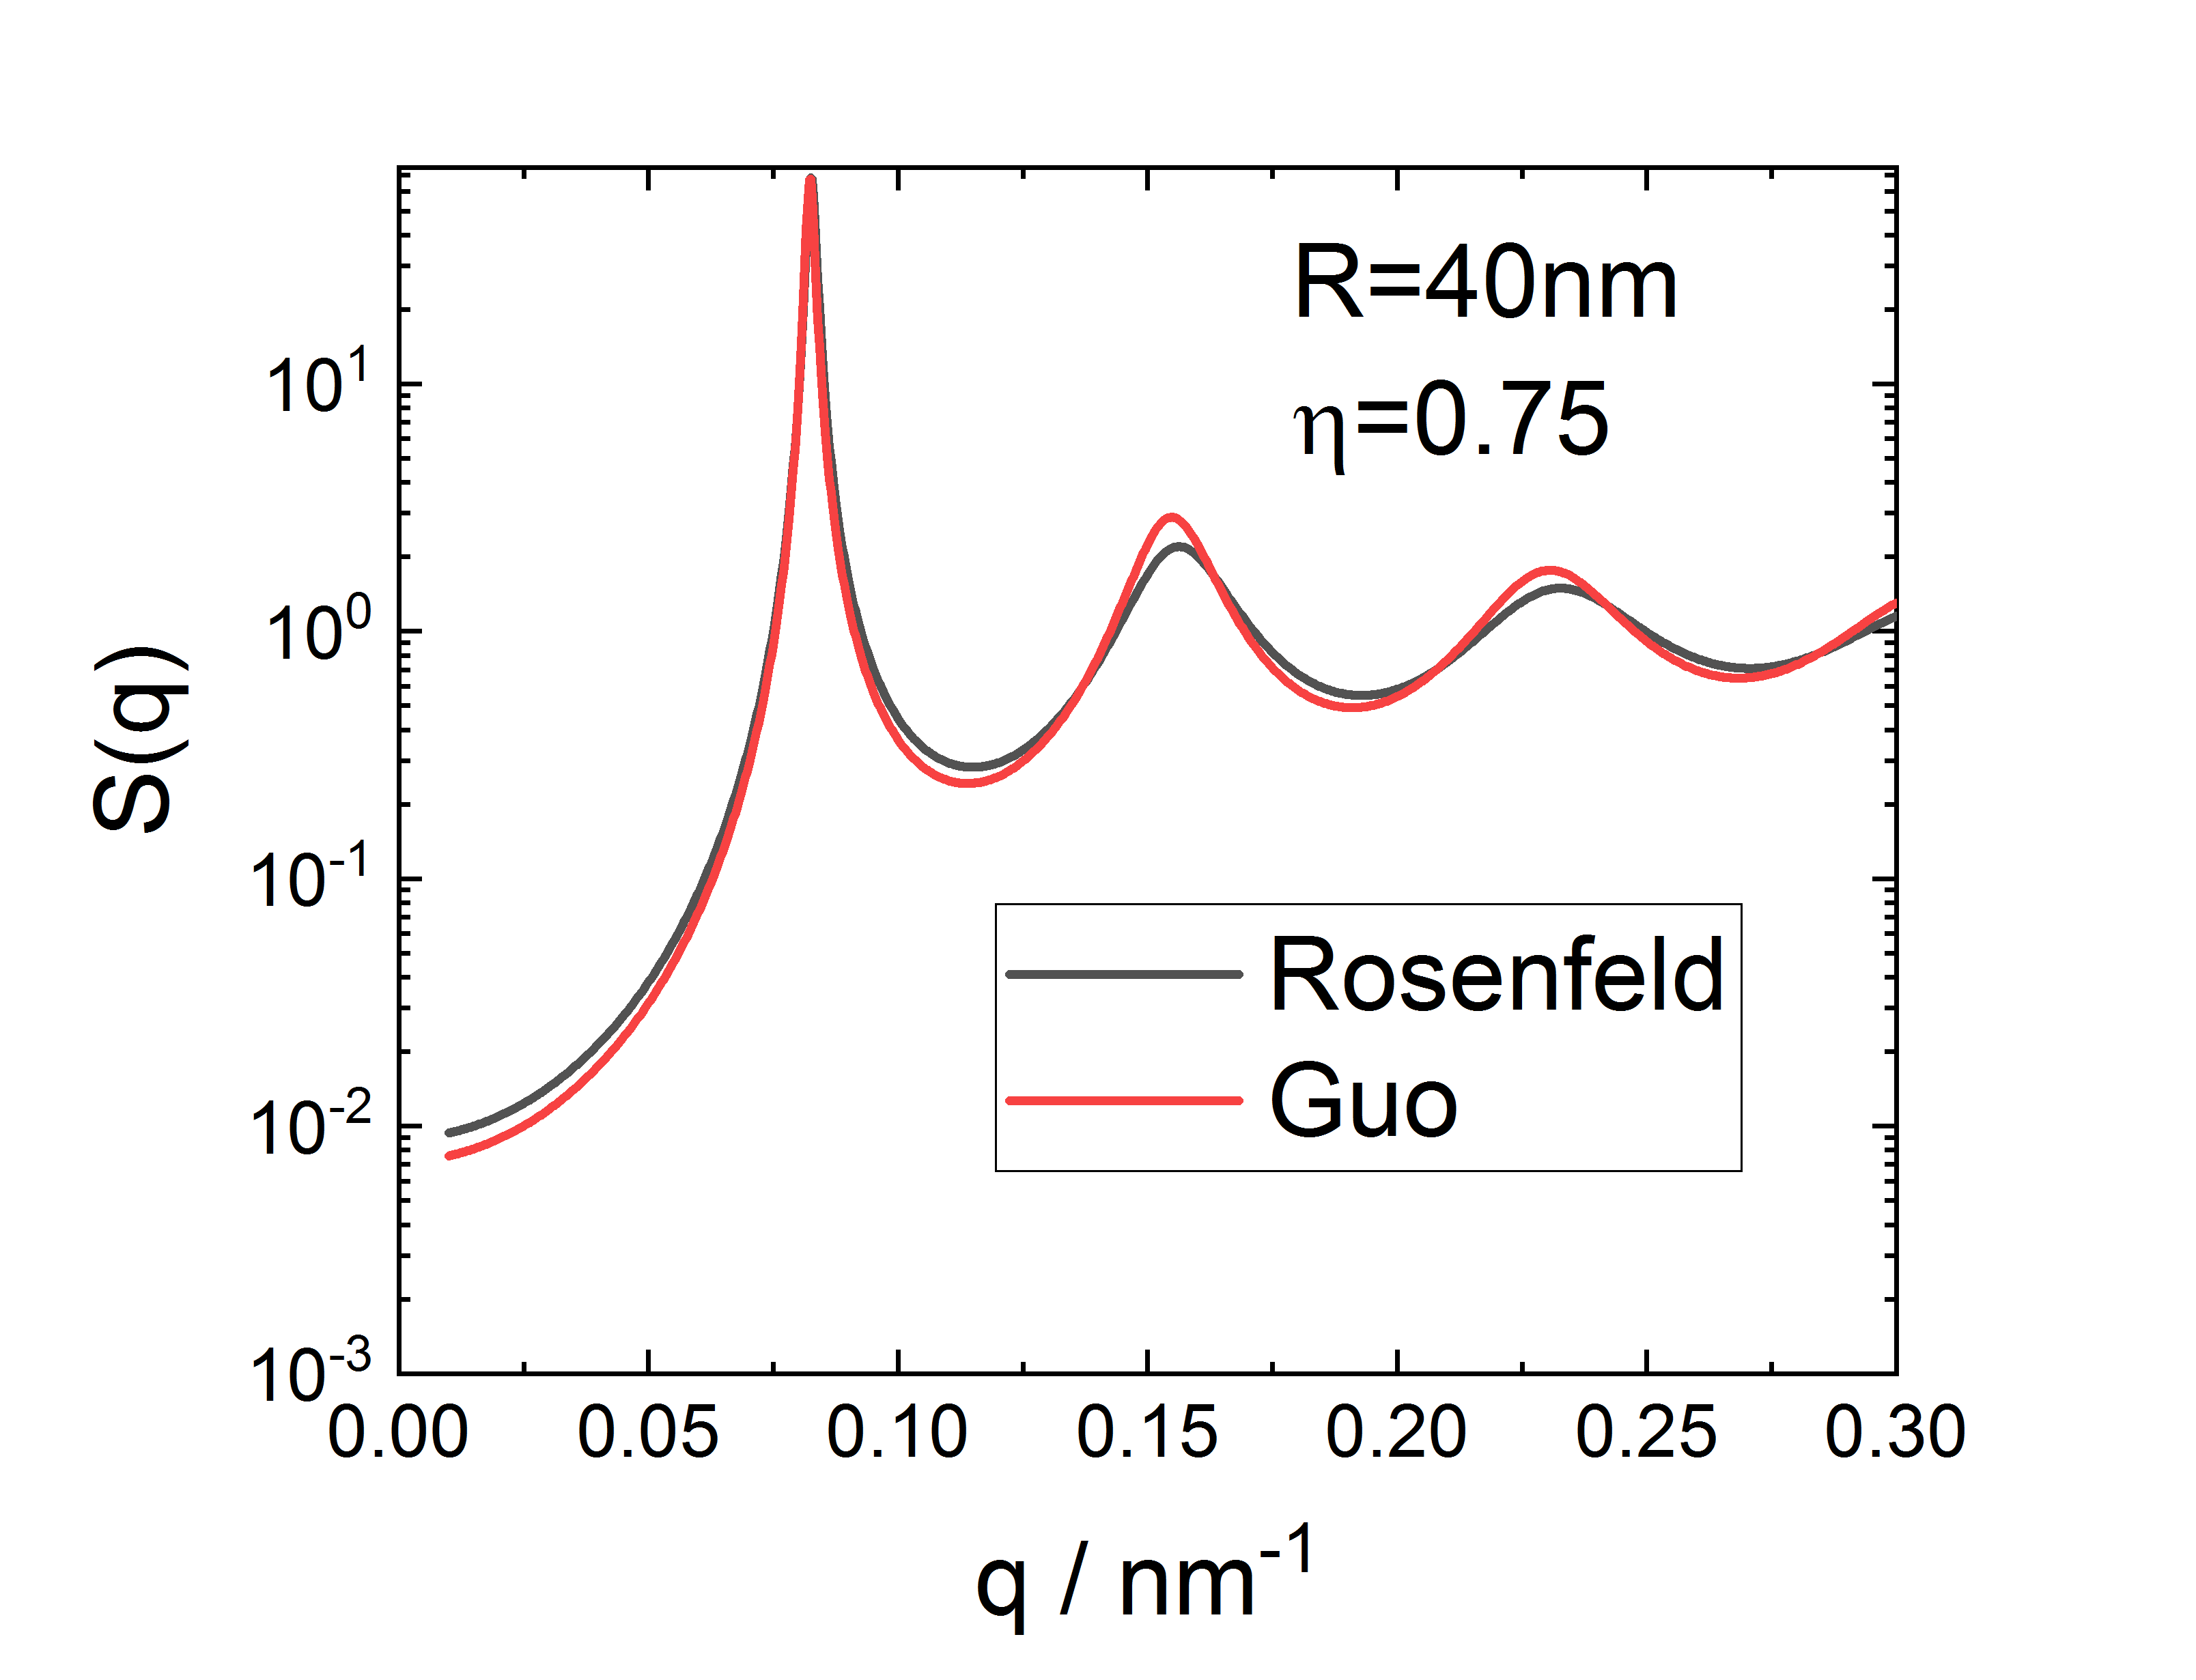
\includegraphics[width=1\textwidth]{../images/structure_factor/2D_hard_disk_fluid/HardDisks_high.png}
   \caption{surface coverage of $\eta=0.75$}
   \label{fig:RosenfeldGuo2}
\end{subfigure}
  \caption{Comparison between Rosenfeld's and Guo's results}
  \label{fig:RosenfeldGuo}
\end{figure}

\clearpage
\section{One dimensional structure factors}

for one dimensional structure factors the relative orientation of the 1D structure to the detection plane is relevant. The orientation has been defined by spherical coordinates with the polar axis pointing in the horizontal direction of the detection plane.
\begin{figure}[htb]
\begin{center}
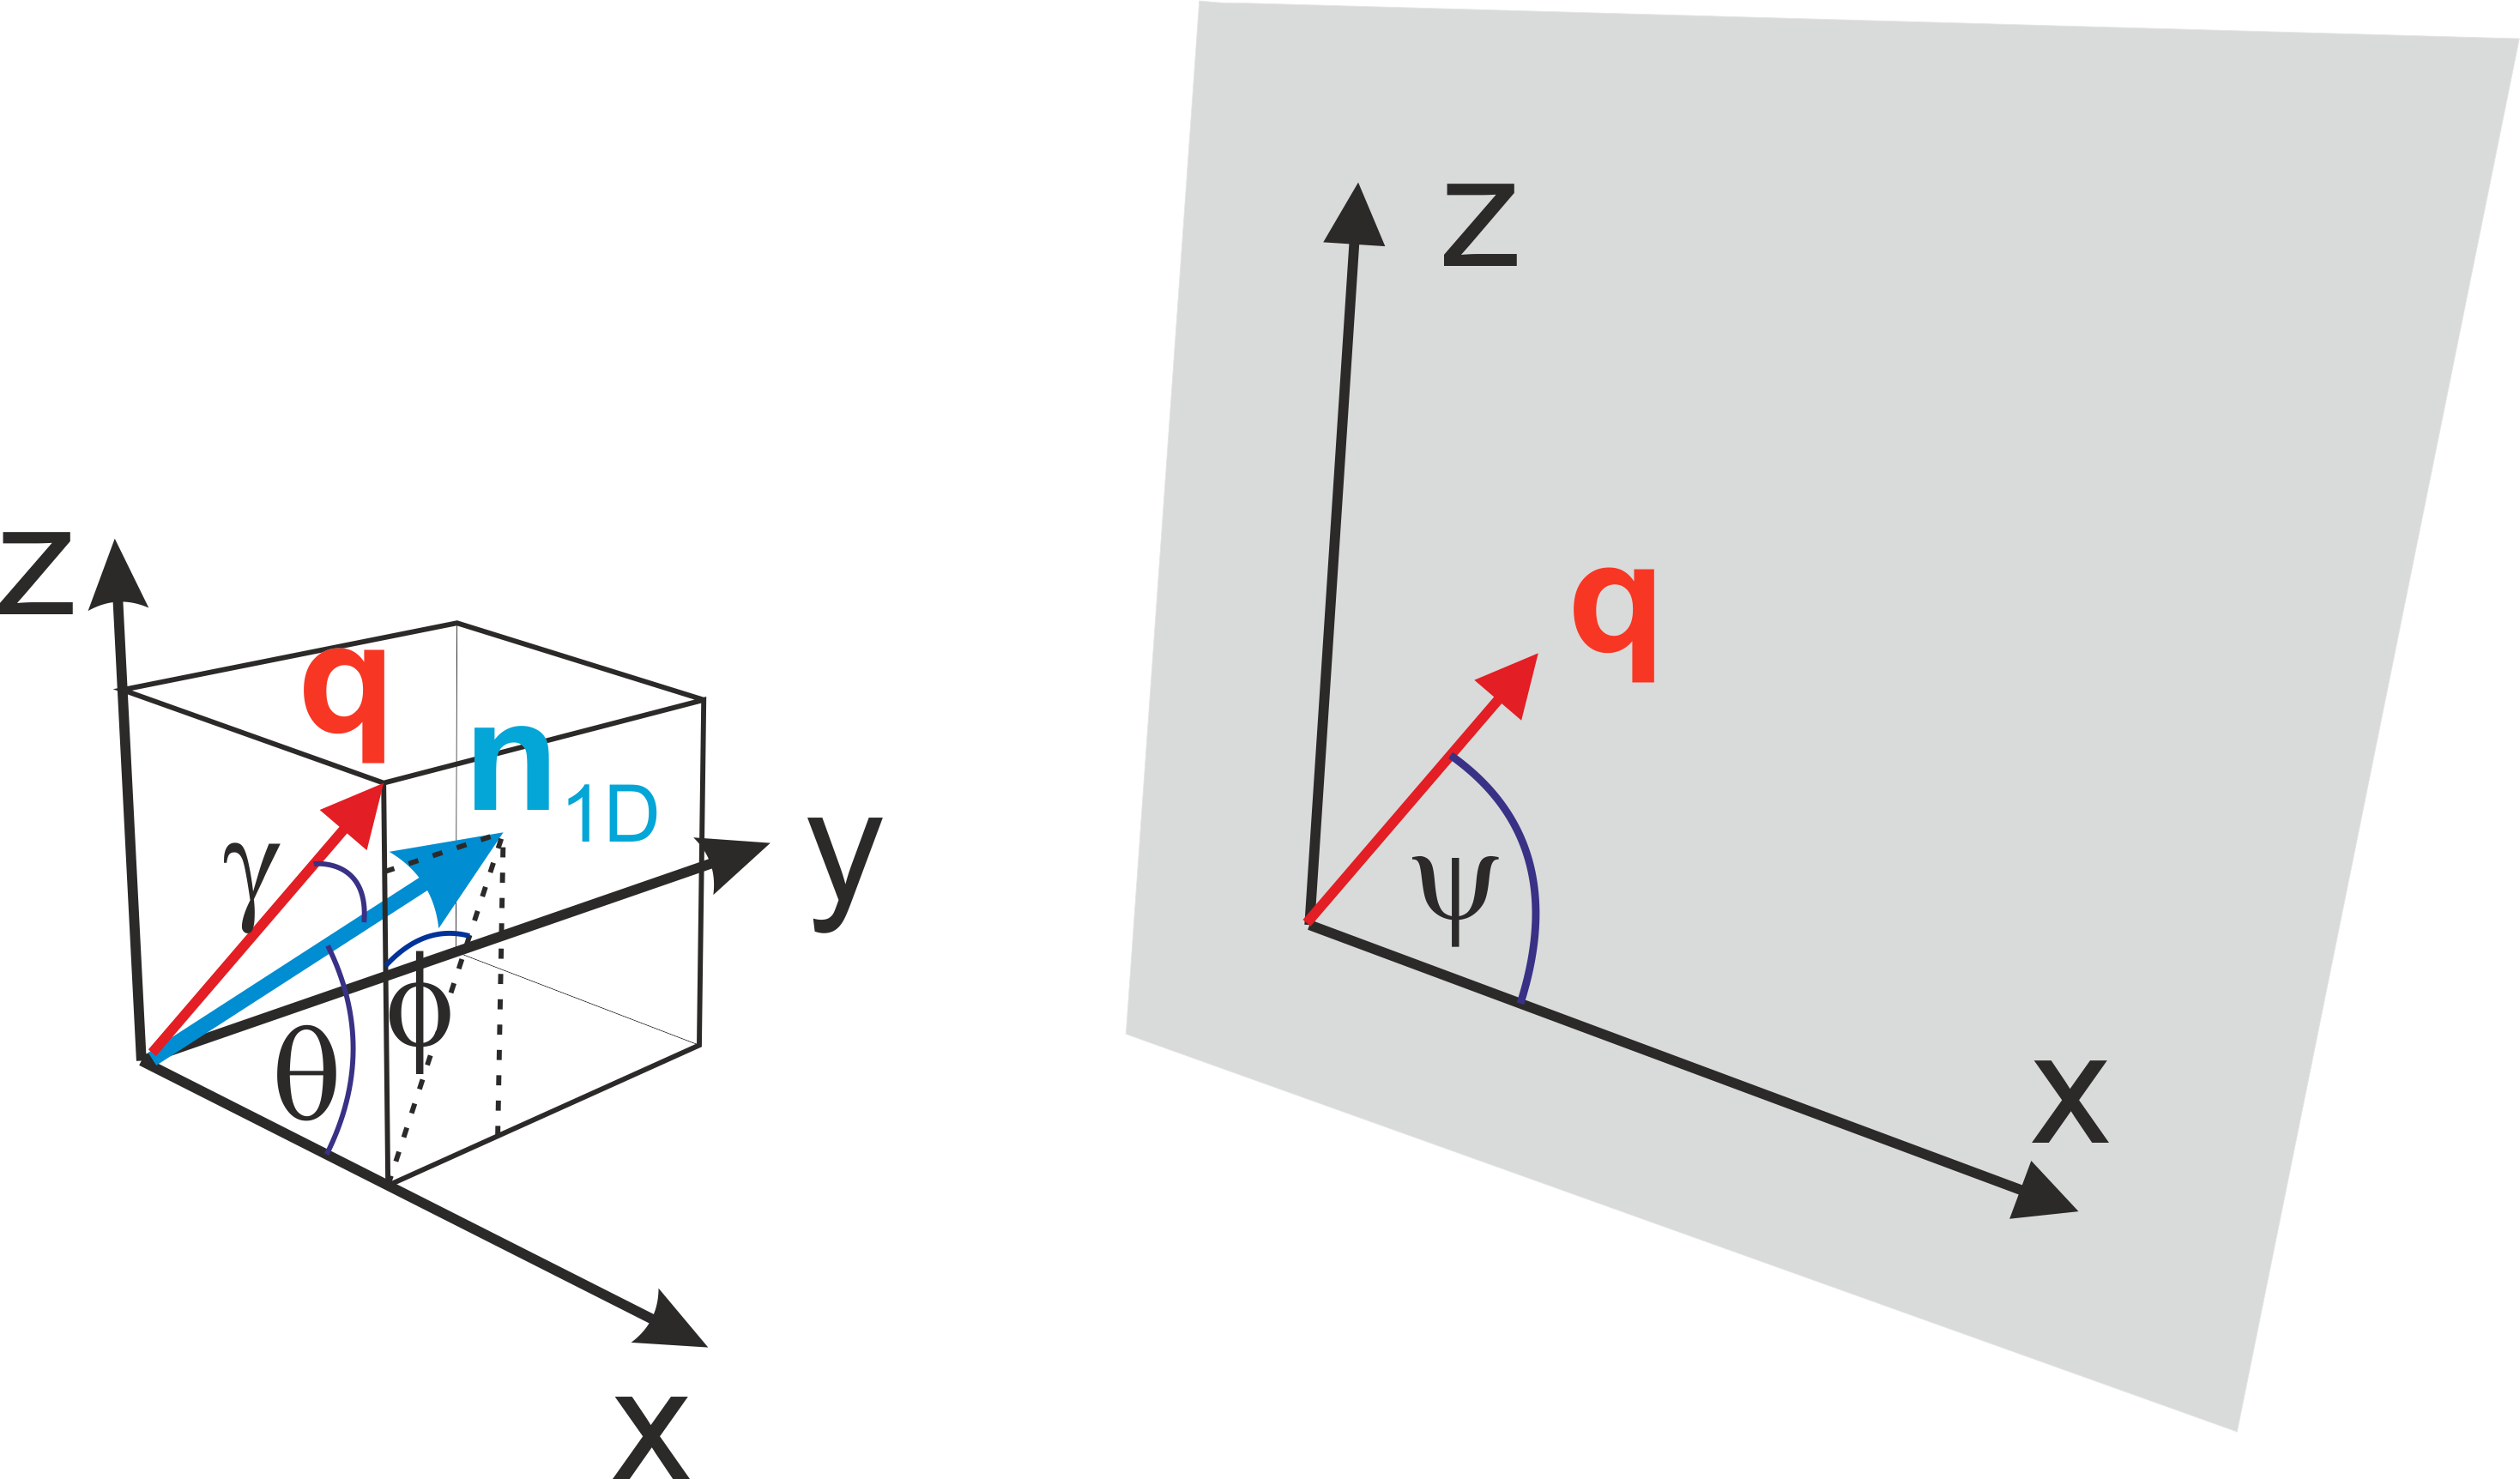
\includegraphics[width=0.75\textwidth]{../images/structure_factor/SQ_1D_2D/coord_SQ_1D.png}
\end{center}
\caption{coordination system for 1D structure factors relative to the detection plane.}
\label{fig:coord1DSQ}
\end{figure}
With the following definition for the scattering vector and the unit vector defining the direction of the 1D structure
\begin{align}
  \mathbf{q} &=q  \begin{pmatrix}
               \cos \psi \\
               0 \\
               \sin \psi \\
             \end{pmatrix}
   \mbox{~~and~~}
  \mathbf{n}_\mathrm{1D} =
    \begin{pmatrix}
        \cos \theta \\
        \sin \theta \sin \phi  \\
        \sin \theta \cos \phi
    \end{pmatrix} \\
\end{align}
the angle $\gamma$ between $\mathbf{q}$ and $ \mathbf{n}_\mathrm{1D}$ is given as
\begin{align}
  \cos\gamma &= \cos\psi\cos\theta+\sin\psi\sin\theta\cos\phi
\end{align}

\subsection{Structure factor for a hard spheres potential in one dimension} \hspace{1pt}

The structure factor for hard spheres in one dimension has been solved in \cite{Leutheusser1984} and also implemented in the open source software \texttt{Jscatter} \cite{Biehl2019}. The structure factor is given by
\begin{align}
\label{eq:SQ_HS_1D}
  S_\mathrm{HS,1D,||}(q,\sigma,\eta) & = \frac{1}{1-\frac{\eta}{\sigma} \tilde{c}(q)} \\
\label{eq:cQ_HS_1D}
  \tilde{c}(q) &= -2\left(A(q)+B(q)\right) \\
  A(q) &= \frac{\sigma}{1-\eta} \frac{\sin q\sigma}{q\sigma} \\
  B(q) &= \frac{\eta}{\sigma}\frac{1}{\left(q\left(1-\eta\right)\right)^2}\left[1-\cos q\sigma\right]
\end{align}
The above equation assumes that $\mathbf{q}$ points along the one dimensional structure. In case of a certain angle $\gamma$, with $\cos \gamma=\mathbf{q}\cdot\mathbf{n}_\mathrm{1D}/(\abs{\mathbf{q}}\,\abs{\mathbf{n}_\mathrm{1D}})$, between $\mathbf{q}$ and the direction $\mathbf{n}_\mathrm{1D}$ of the one dimensional structure one has to take
\begin{align}
\label{eq:SQ_HS_1D}
  S_\mathrm{HS,1D}(q,\sigma,\eta,\gamma) & = S_\mathrm{HS,1D,||}(q\cos\gamma,\sigma,\eta)
\end{align}
For random oriented 1D structures the orientational average of the structure factor needs to be done in principle together with the form factor as shown for example in section \ref{sect:StackedDiscs} for stacked discs. However, if the individual stacked structures are spherical symmetric like a straight chain of spheres the form factor is isotropic and the average can be performed over the structure factor only which then reads as
\begin{align}
\label{eq:SQ_HS_1D_random}
  S_\mathrm{HS,1D,ran}(q,\sigma,\eta,\gamma) & = \int_0^1 S_\mathrm{HS,1D,||}(qx,\sigma,\eta) \, \mathrm{d}x
\end{align}

\subsection{One dimensional paracrystal}  \hspace{1pt}

\begin{align}\label{eq:SQ1D_paracrystal}
  S(q,\gamma) &=  1+\frac{2}{n} \sum_{k=1}^{n-1} (n-k)
\cos(kDq\cos(\Theta))
     \exp\left(-\frac{k}{2}\left(q\cos(\Theta) \sigma_D\right)^2\right)
\end{align}

\begin{figure}[htb]
\begin{center}
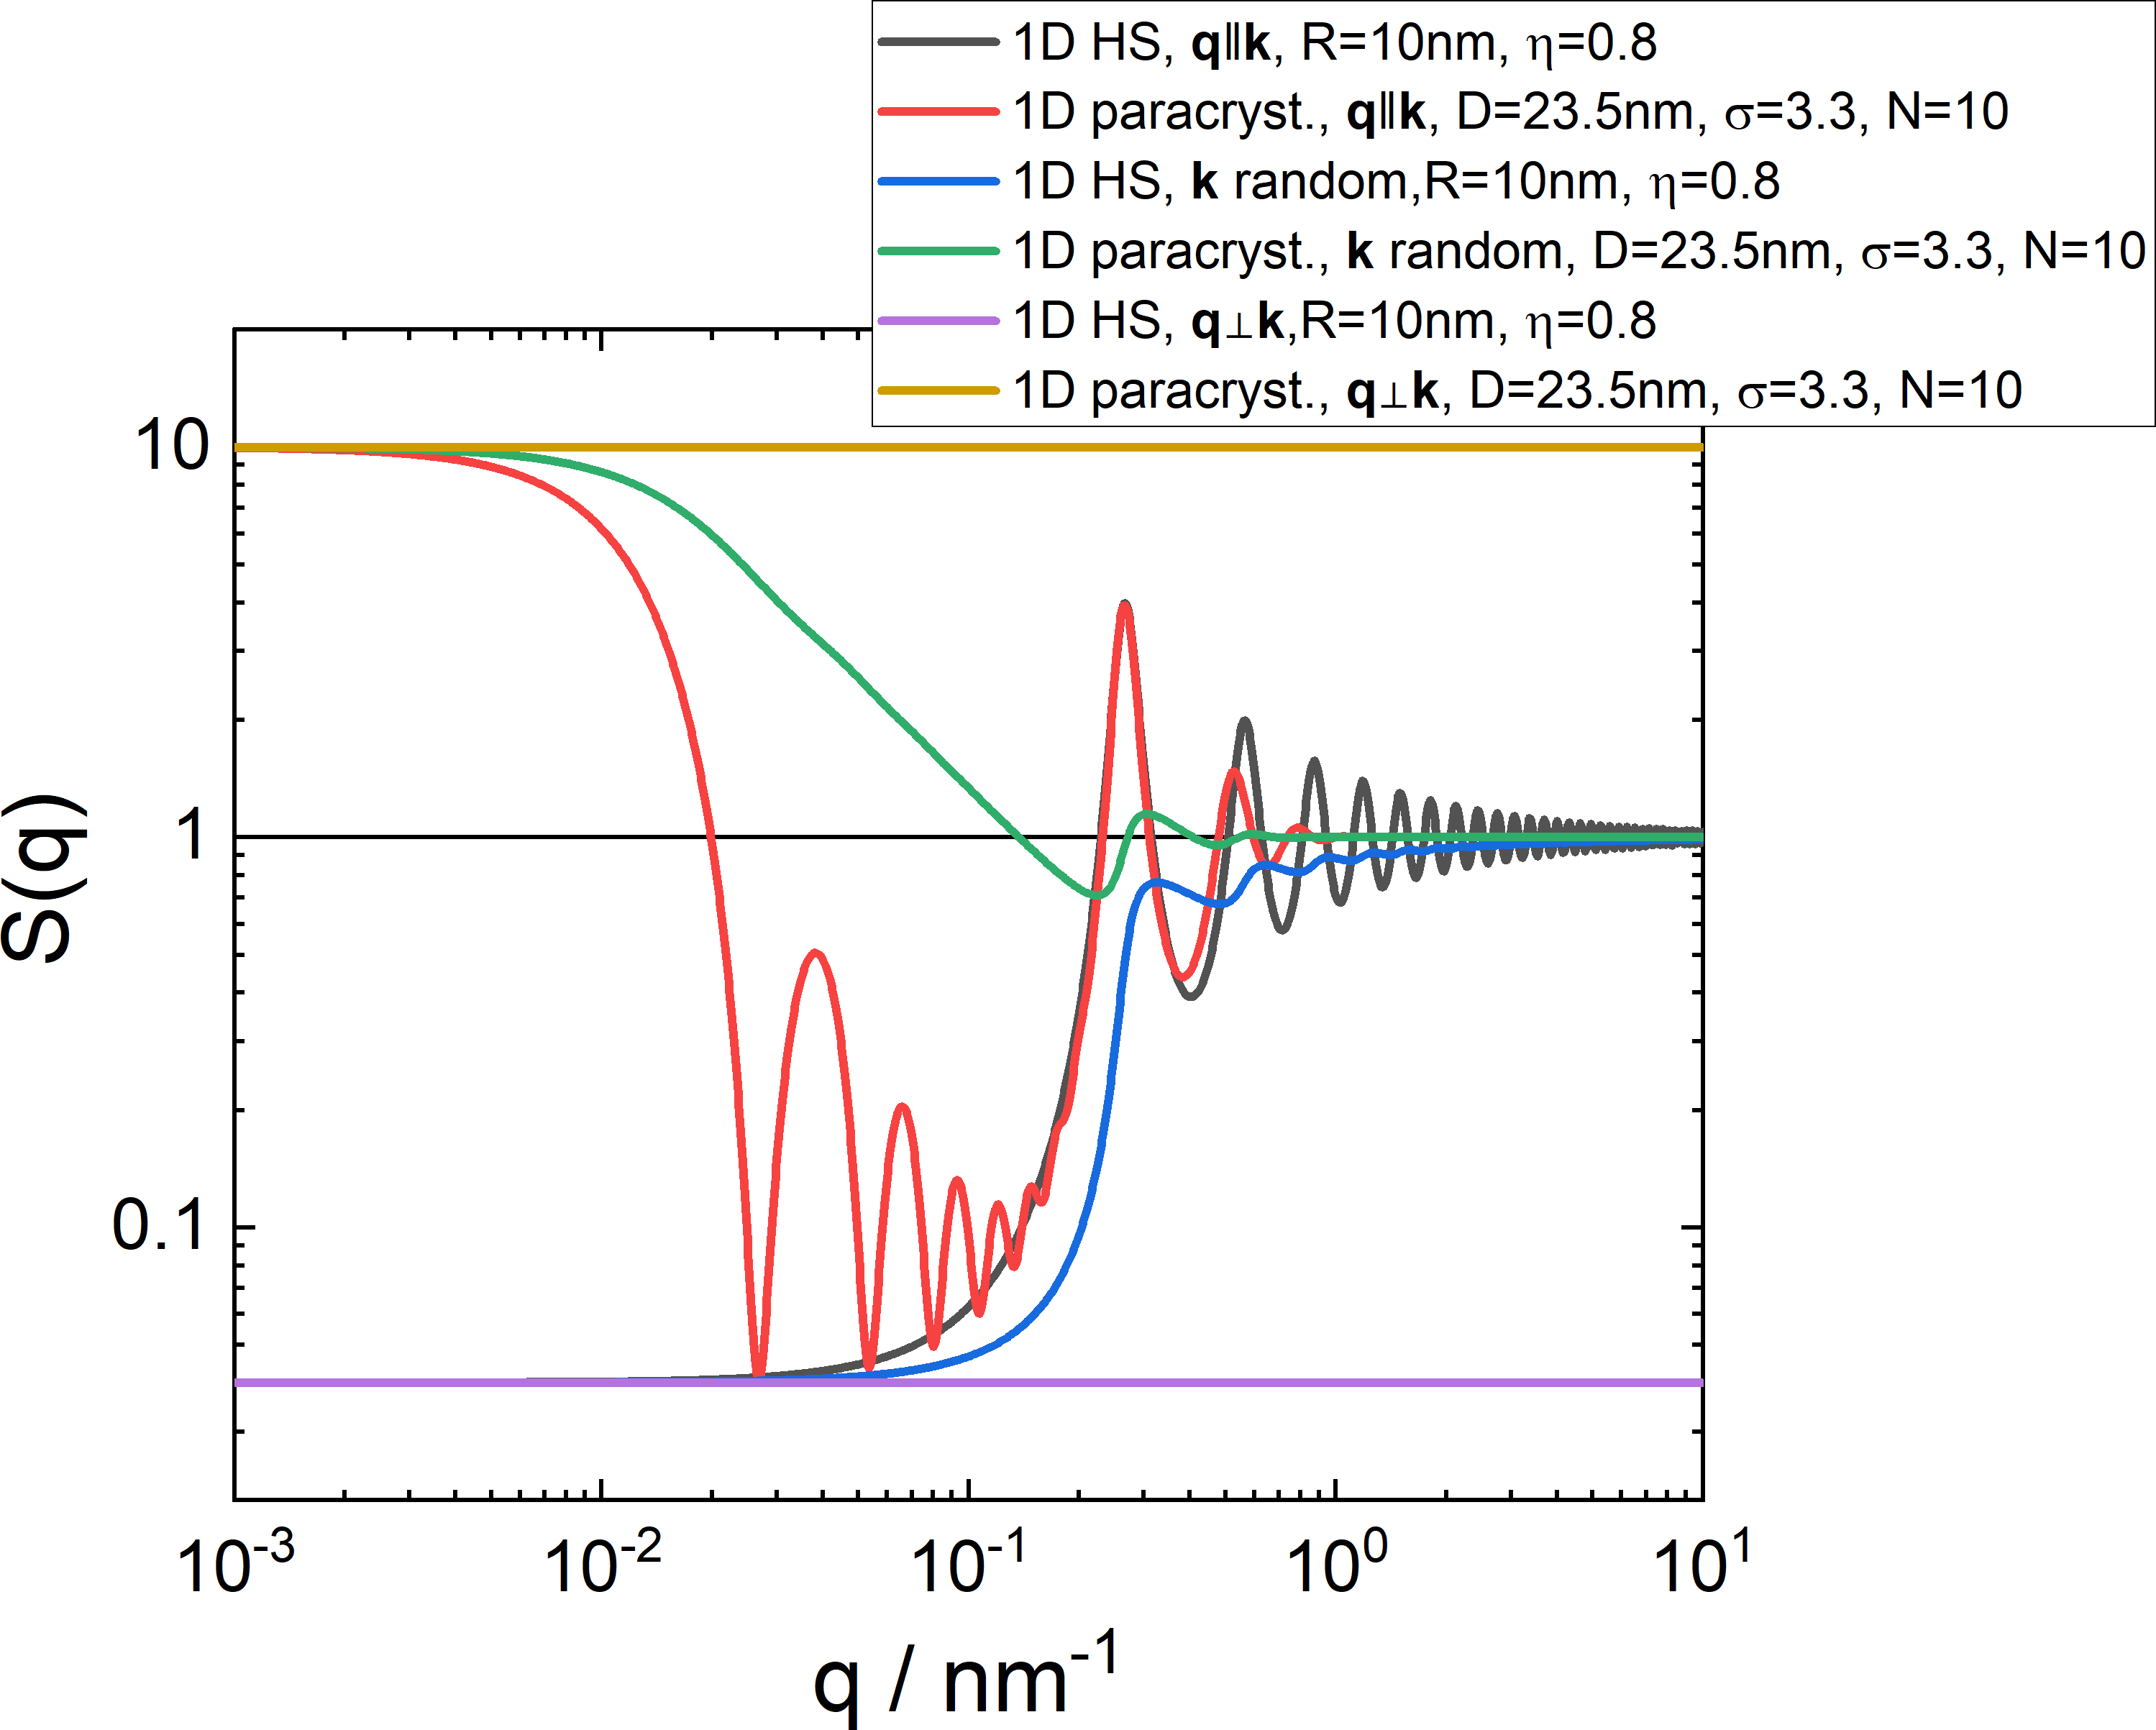
\includegraphics[width=0.75\textwidth]{../images/structure_factor/SQ_1D_2D/SQ_1D.png}
\end{center}
\caption{structure factor of aligned for both q parallel and perpendicular to the direction of the 1D structure as well as and random oriented 1D structures.}
\label{fig:1DSQ}
\end{figure}

\clearpage
%%%%%%%%%%%%%%%%%%%%%%%%%%%%%%%%%%%%%%%%%%%%%%%%%%%%%%%%%%%%%%%%%%%%%%%%%%%%%%%%%%%%%%%%
\section{three dimensional structure factor for sticky hard sphere systems} \hspace{1pt}
\label{sec:sHS}

\subsection{Sticky Hard Sphere} ~\\

In Baxter's model \cite{Baxter1968,Robertus1989,Kruif1989,Barboy1974,Menon1991,Menon1991a}
of adhesive hard spheres the pair interaction potential $U(r)$ is replaced by
\begin{equation}
\frac{U(r)}{k_BT} =
 \begin{cases}
      \infty    & \text{for} \quad 0<r<\sigma \\
      \ln\frac{12\tau\Delta}{\sigma+\Delta} & \text{for} \quad \sigma<r<\sigma+\Delta \\
      0         & \text{for} \quad r>\sigma+\Delta
   \end{cases}
\end{equation}
after which, when applied, the limit $\Delta \to 0$ is taken.
Thus, only a single parameter, the so-called stickiness parameter
$\tau$, characterizes the adhesive strength.
\begin{subequations}
\begin{align}
\kappa &= 2 q R_\text{HS} \\
\eta &= f_p \left(\frac{2R_\text{HS}+\Delta}{2R_\text{HS}}\right)^3\\
\epsilon &= \tau+\frac{\eta}{1-\eta} \\
\gamma &= f_p\frac{1+\eta/2}{3\left(1-\eta\right)^2} \\
\lambda &= \frac{6}{\eta} \left(\epsilon-\sqrt{\epsilon^2-\gamma}\right) \label{eq:sHS_lambda}\\
\mu &= \lambda \eta (1-\eta) \\
\beta &= -\frac{3\eta \left(2+\eta\right)^2-2\mu \left(1+7\eta+\eta^2\right)+\mu^2(2+\eta)}{2\left(1-\eta\right)^4}\\
\alpha &= \frac{\left(1+2\eta-\mu\right)^2}{\left(1-\eta\right)^4}\\[5mm]
C(q) = & 2\frac{\eta\lambda}{\kappa}\sin\kappa
        -2\frac{\eta^2\lambda^2}{\kappa^2}\left(1-\cos\kappa\right) -\\
   \Big\{ & \alpha\kappa^3(\sin\kappa-\kappa\cos\kappa)
           +\beta\kappa^2(2\kappa\sin\kappa-(\kappa^2-2)\cos\kappa-2)\nonumber\\
          & +\frac{\eta\alpha}{2}\left((4\kappa^3-24\kappa)\sin\kappa-(\kappa^4-12\kappa^2+24)\cos\kappa+24\right)
             \Big\} \;\times\;24\frac{\eta}{\kappa^6}\nonumber
\end{align}
\begin{align}
   S_\text{sHS}(q,R_\text{HS},f_p,\tau) & = \frac{1}{1-C(q)}
\end{align}
\end{subequations}

\begin{figure}[htb]
\begin{center}
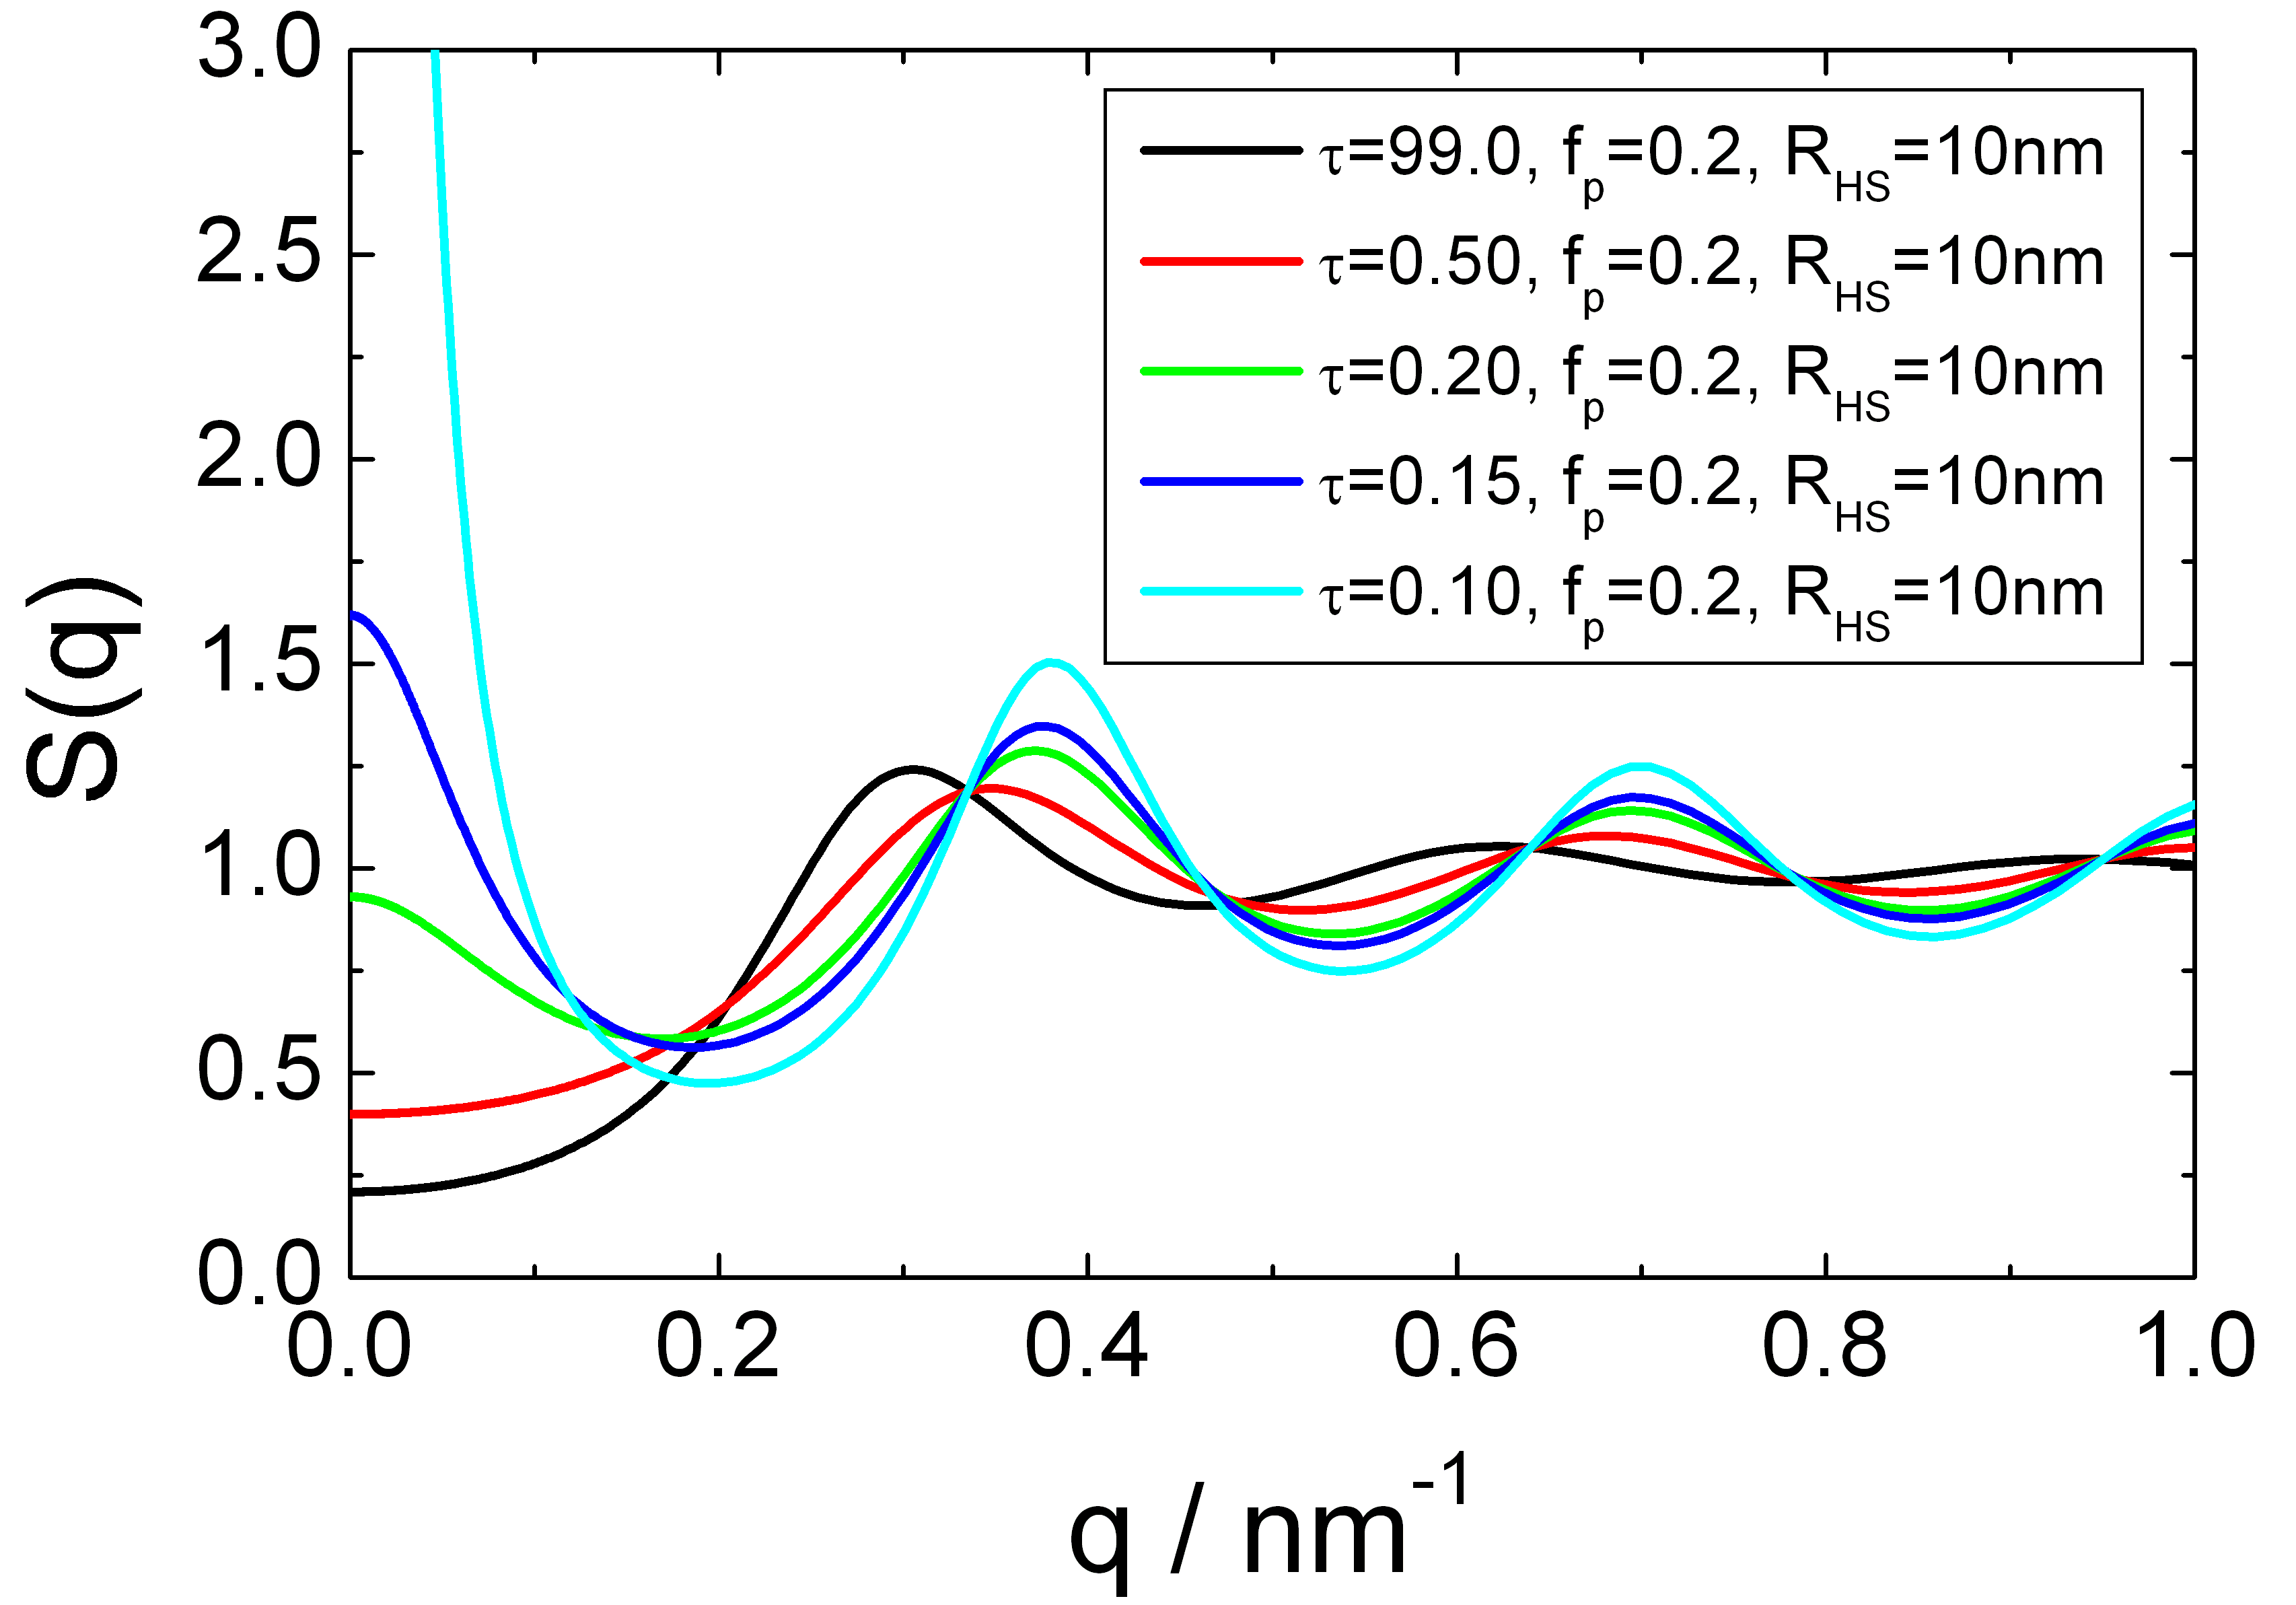
\includegraphics[width=0.768\textwidth]{../images/structure_factor/HardSphere/StickyHardSphere1.png}
\end{center}
\caption{Structure factor $S(q)$ for a sticky hard sphere interaction potential for the different
stickiness parameters $\tau$.}
\label{fig:SQStickyHardSphere1}
\end{figure}

~\\
\uline{Input Parameters for the structure factor model \texttt{sticky hard sphere}:}
\begin{description}
\item[\texttt{RHS}] hard sphere radius
\item[\texttt{fp}] volume fraction $f_p$
\item[\texttt{tau}] stickiness parameter $\tau$
\end{description}

\noindent\uline{Note:}
\begin{itemize}
\item for stickiness parameters close to zero the root in eq.\ \ref{eq:sHS_lambda} becomes complex and is considered as a critical point where the system phase separates.
\end{itemize}


%%%%%%%%%%%%%%%%%%%%%%%%%%%%%%%%%%%%%%%%%%%%%%%%%%%%%%%%%%%%%%%%%%%%%%%%%%

\subsection{Sticky Hard Sphere ($2^\text{nd}$ version)}~\\

In Baxter's model of adhesive hard spheres the pair interaction
potential $U(r)$ is replaced by
\begin{equation}
\frac{U(r)}{k_BT} =
 \begin{cases}
      \infty    & \text{for} \quad 0<r<\sigma-\Delta \\
      \ln\frac{12\tau\Delta}{\sigma+\Delta} & \text{for} \quad \sigma-\Delta<r<\sigma \\
      0         & \text{for} \quad r>\sigma
   \end{cases}
\end{equation}
The structure factor for this potential has been implemented according to  \cite{Regnaut1989,Regnaut1990} as
\begin{align}
\sigma &= 2R_\text{HS}+\Delta \\
\kappa & = q \sigma \\
\phi   &= f_p \left(\frac{\sigma}{2R_\text{HS}}\right)^3 \\
\lambda_{\pm} & =6 \left(\frac{\tau}{\phi}+\frac{1}{1-\phi}\right)
                \pm \sqrt{
                    36 \left[
                        \frac{\tau}{\phi}+\frac{1}{1-\phi}
                      \right]^2
                   -\frac{12}{\phi}\frac{1+\frac{\phi}{2}}{\left(1-\phi\right)^{2}}
                } \label{eq:sHS2_lambda}\\
   \lambda & =
       \begin{cases}
           \lambda_+ & \mbox{for }\lambda_+ < \abs{\lambda_-} \\
           \lambda_- & \mbox{otherwise}
       \end{cases}
\end{align}
\begin{align}
\mu & = \lambda \phi (1-\phi) \\
A & = \frac12 \; \frac{1+2 \phi-\mu}{\left(1-\phi\right)^2} \\
B & = \frac{\sigma}{2} \frac{\mu-3\phi}{2 \left(1-\phi\right)^2 } \\
C & = -A\sigma^2-B\sigma+\lambda\sigma^2/12
\end{align}
\begin{align}
I_n(\kappa) &= \int_0^1 x^n \cos(\kappa x)\; dx \\
J_n(\kappa) &= \int_0^1 x^n \sin(\kappa x)\; dx \\
\alpha & = 1-12 f_p \left( C\sigma^{-2}I_0(\kappa) + B\sigma^{-1} I_1(\kappa) +AI_2(\kappa) \right)\\
\beta  &=    12 f_p \left( C\sigma^{-2}J_0(\kappa) + B\sigma^{-1} J_1(\kappa) +AJ_2(\kappa) \right) \\
S(Q) & = \frac{1}{\alpha^2+\beta^2}
\end{align}


\begin{figure}[htb]
\begin{center}
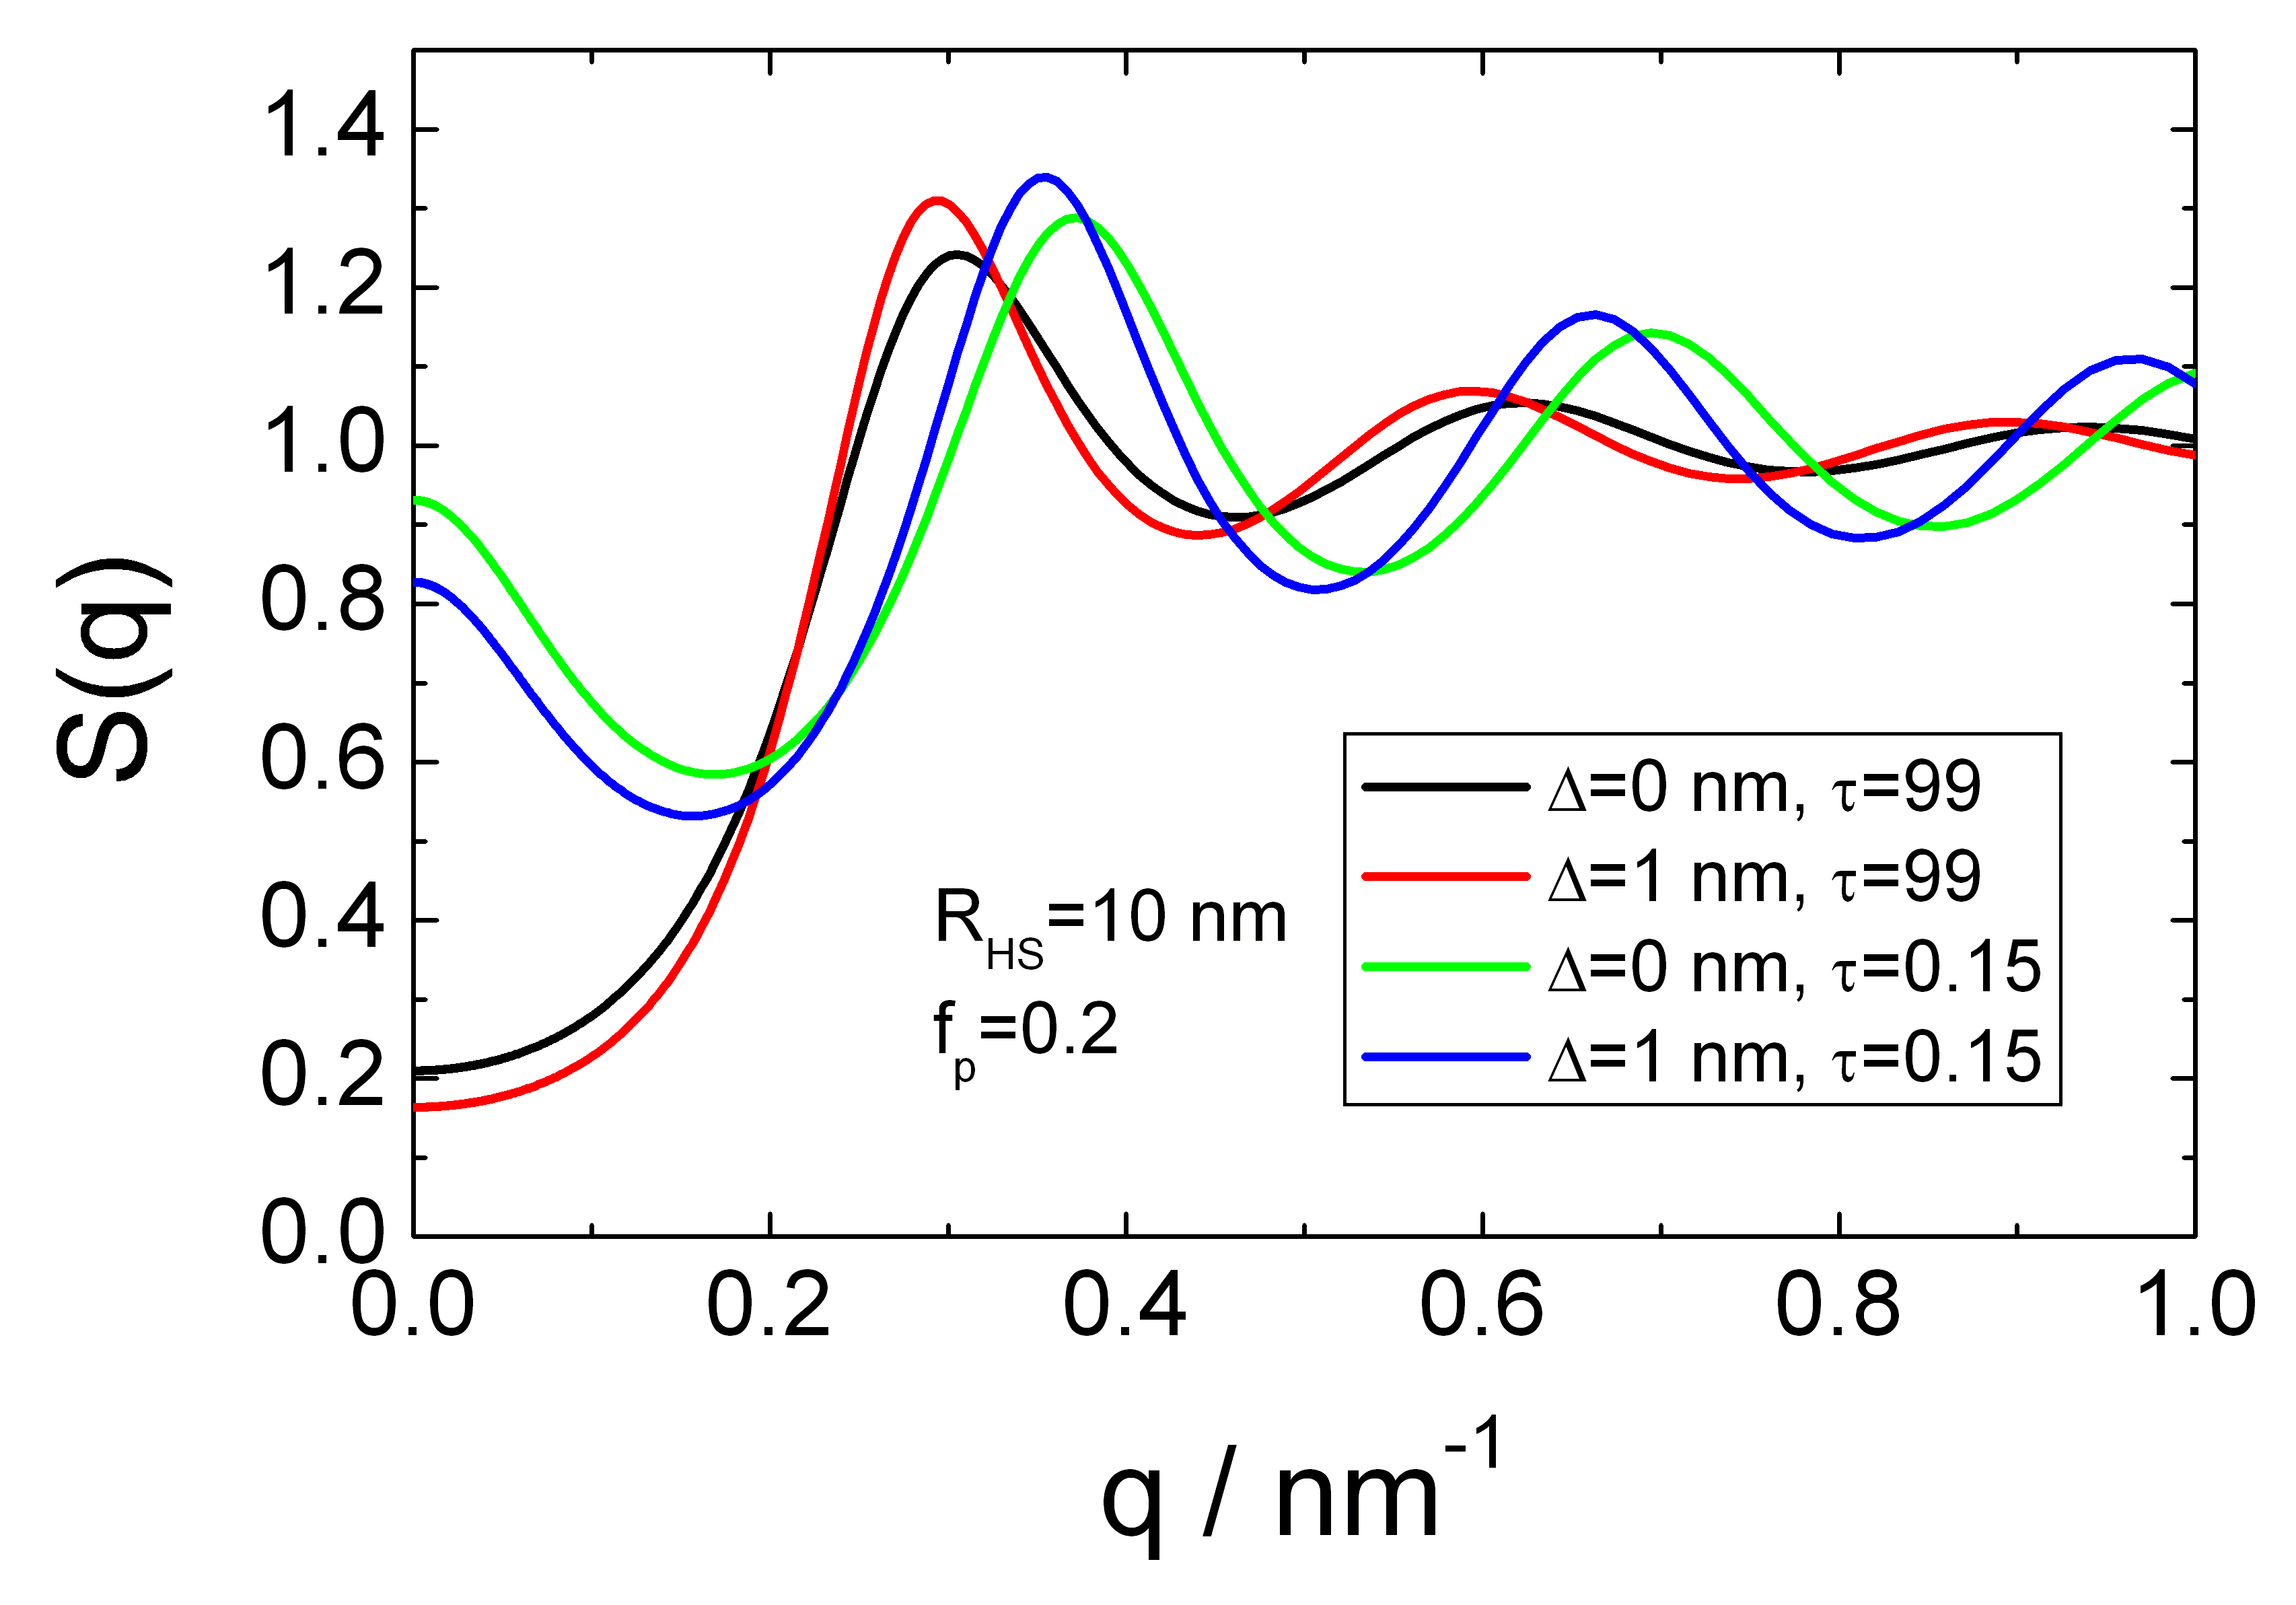
\includegraphics[width=0.768\textwidth]{../images/structure_factor/HardSphere/StickyHardSphere2.png}
\end{center}
\caption{Structure factor $S(q)$ for a sticky hard sphere interaction potential for the different
stickiness parameters $\tau$.}
\label{fig:SQStickyHardSphere2}
\end{figure}

~\\
\uline{Input Parameters for the structure factor model \texttt{Sticky Hard Sphere 2}:}
\begin{description}
\item[\texttt{RHS}] hard sphere radius
\item[\texttt{fp}] volume fraction $f_p$
\item[\texttt{tau}] stickiness parameter $\tau$
\item[\texttt{Delta}] width $\Delta$ of stickiness potential
\end{description}

\noindent\uline{Note:}
\begin{itemize}
\item for stickiness parameters close to zero the root in eq.\ \ref{eq:sHS2_lambda} becomes complex and is considered as a critical point where the system phase separates.
\end{itemize}


\subsection{Square Well Potential}  ~\\

The Square well potential can be written as
\begin{equation}
U(r) =
 \begin{cases}
      \infty    & \text{for} \quad 0<r<\sigma \\
      -\epsilon & \text{for} \quad \sigma<r<\lambda\sigma \\
      0         & \text{for} \quad r>\lambda\sigma
   \end{cases}
\end{equation}
where $\lambda$ and $\epsilon$ correspond to the breadth and the
depth of the square well potential. The structure factor $S(Q)$ is
then given by the following relations \cite{Sharma1977}:
\begin{subequations}
\begin{align}
S(Q)  = & \frac{1}{1-C(Q)} \\
C(Q)  = & - \frac{24\eta}{(Q\sigma)^6} \Big\{ \alpha(Q\sigma)^3
\left[\sin(Q\sigma)-Q\sigma\cos(Q\sigma)\right] \\
        & +\beta(Q\sigma)^2\left[2Q\sigma\sin(Q\sigma)-(Q^2\sigma^2-2)\cos(Q\sigma)-2\right]\nonumber\\
        & +\gamma \left[(4Q^3\sigma^3-24Q\sigma)\sin(Q\sigma)-(Q^4\sigma^4-12Q^2\sigma^2+24)\cos(Q\sigma)+24\right] \nonumber\\
        & -\frac{\epsilon}{k_BT} (Q\sigma)^3\left[\sin(\lambda Q\sigma)-\lambda Q\sigma\cos(\lambda Q\sigma)+Q\sigma\cos(Q\sigma)-\sin(Q\sigma)\right]\Big\} \nonumber
\end{align}
where $\alpha$, $\beta$ and $\gamma$ are given by
\begin{align}
\alpha & = \frac{(1+2\eta)^2+\eta^3(\eta-4)}{(1-\eta)^4} \\
\beta  & = -\frac{1}{3}\eta\frac{18+20\eta-12\eta^2+\eta^4}{(1-\eta)^4} \\
\gamma & =
\frac{1}{2}\eta\frac{(1+2\eta)^2+\eta^3(\eta-4)}{(1-\eta)^4}
\end{align}
\end{subequations}
~\\

\begin{figure}[htb]
\begin{center}
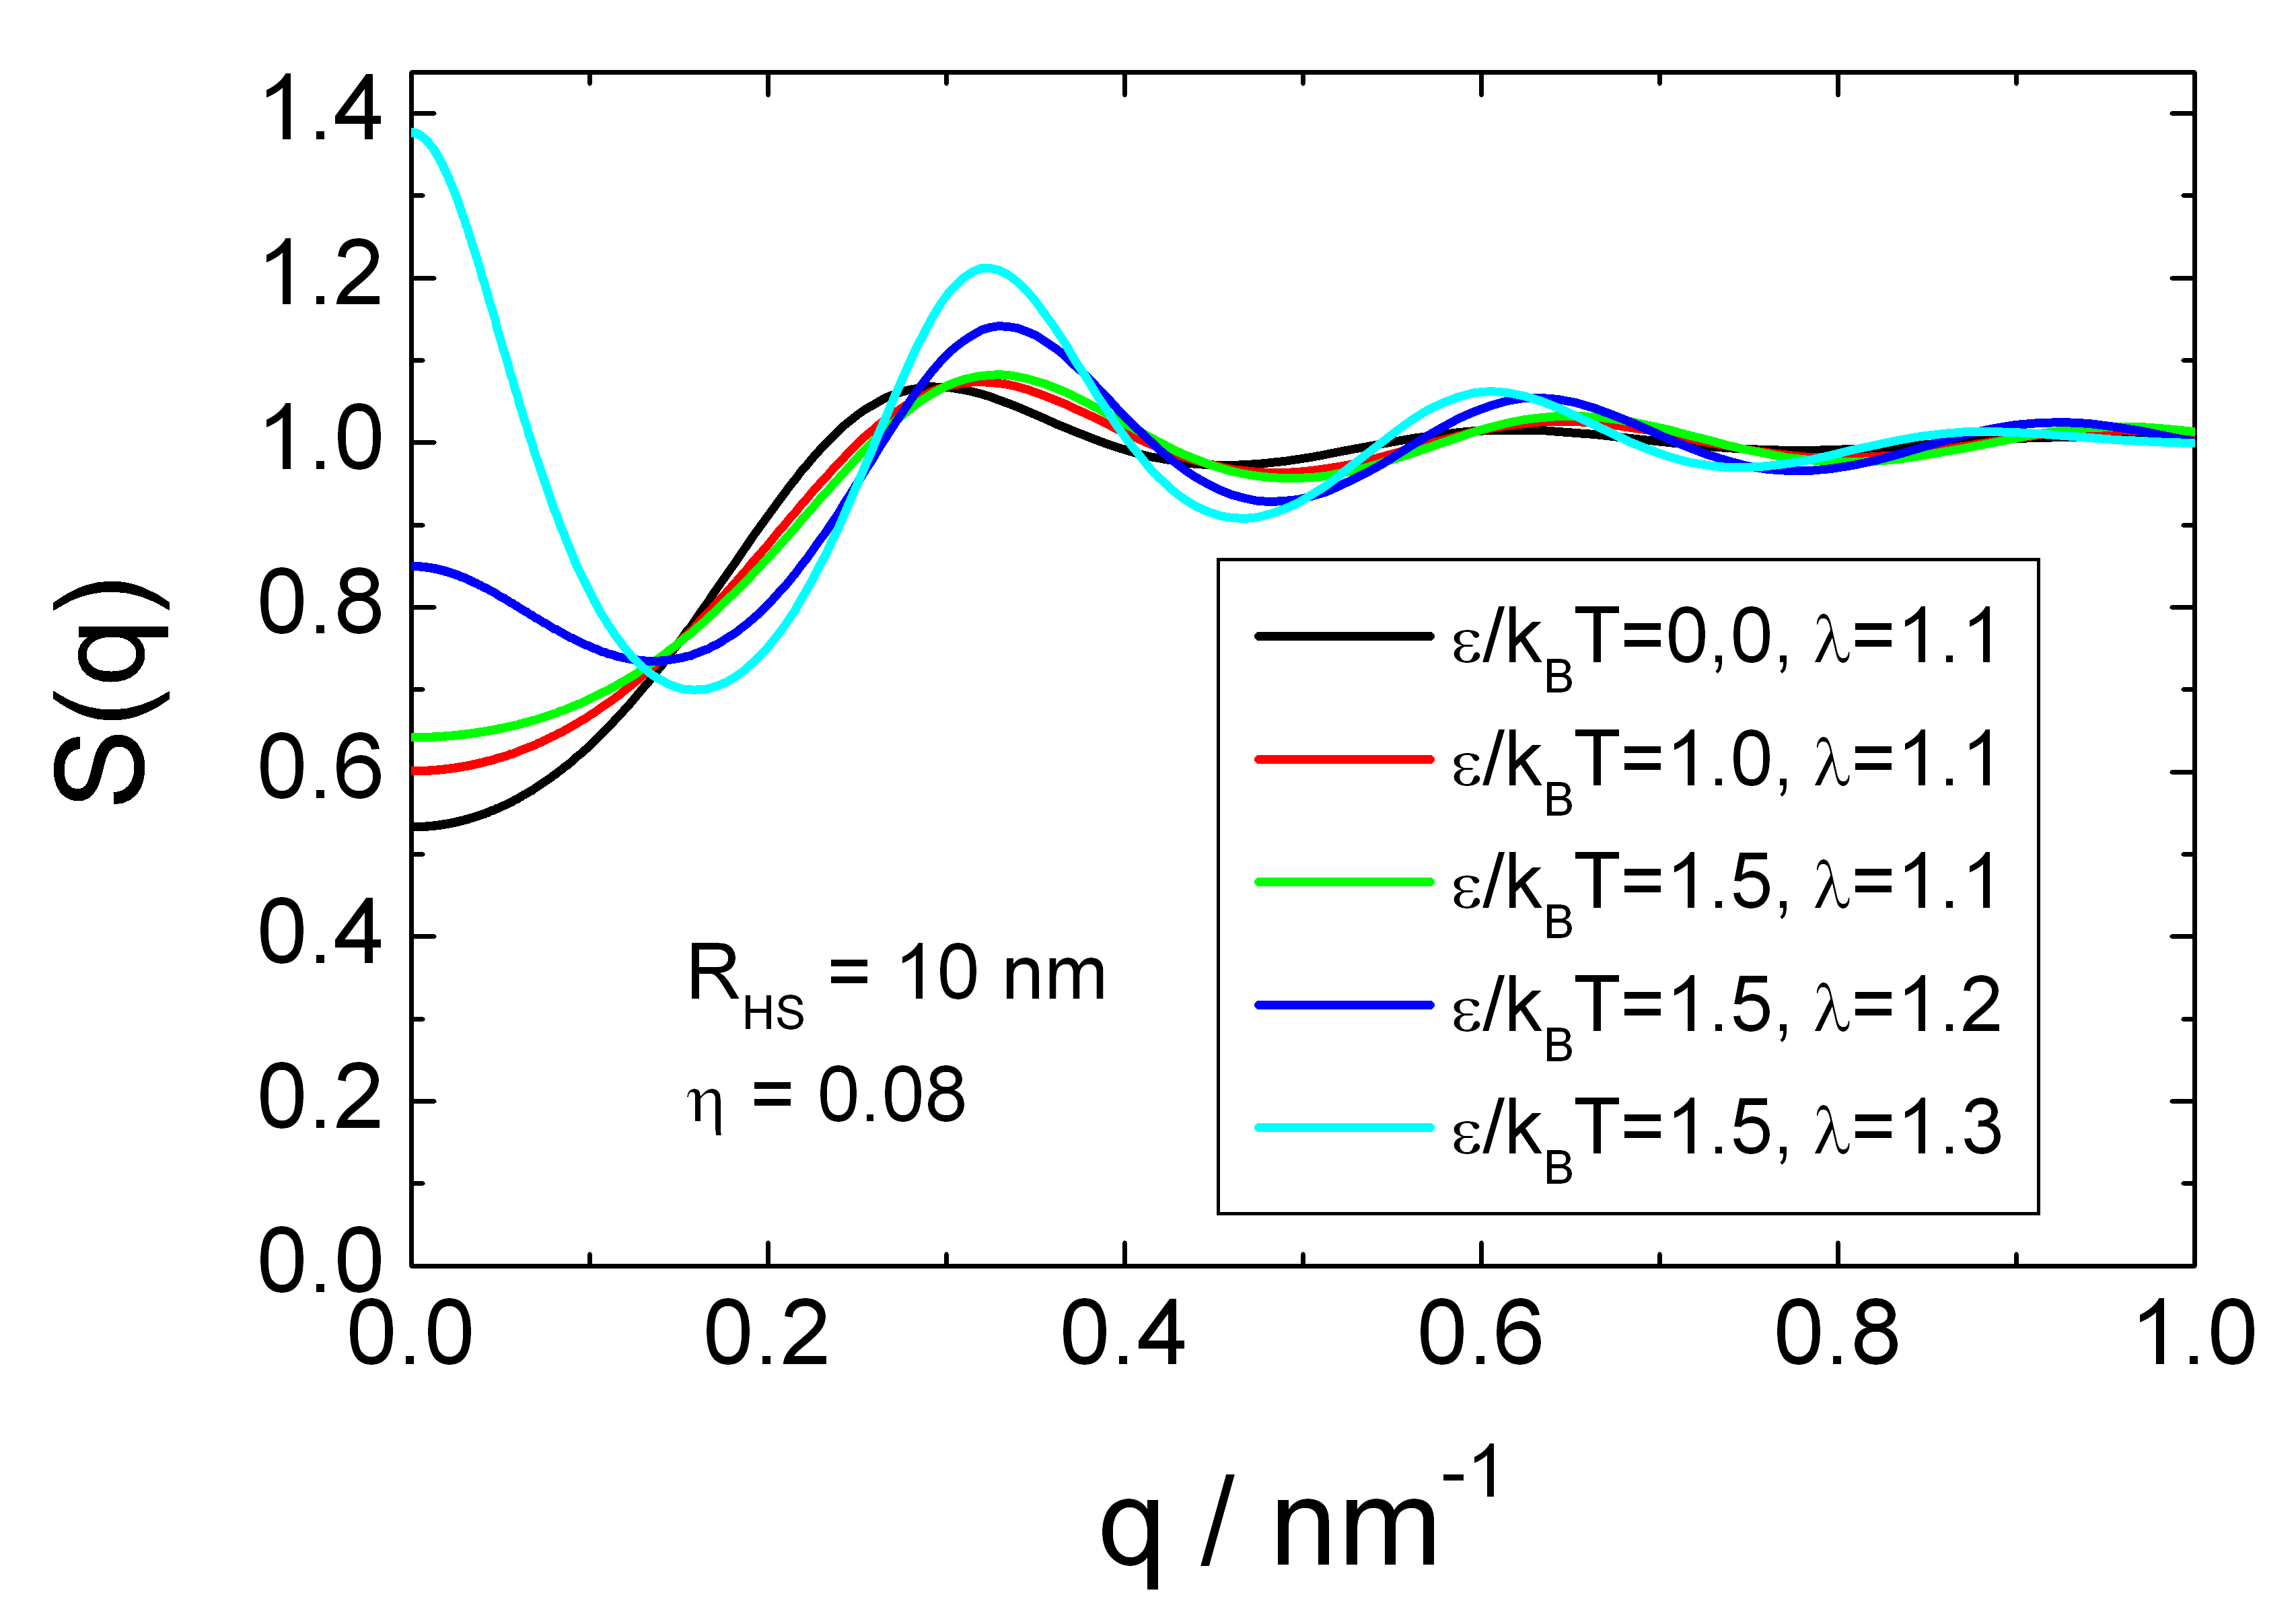
\includegraphics[width=0.768\textwidth]{../images/structure_factor/HardSphere/SquareWellSQ.png}
\end{center}
\caption{Structure factor $S(q)$ for a square well interaction potential.}
\label{fig:SquareWell1}
\end{figure}

~\\
\uline{Input Parameters for the structure factor model \texttt{Square Well Potential}:}
\begin{description}
\item[\texttt{RHS}] hard sphere radius
\item[\texttt{fp}] volume fraction $f_p$
\item[\texttt{epsi/kT}]square well depth $\epsilon/k_BT$ in units of $k_BT$
\item[\texttt{lambda}] relative square well width $\lambda>1$, $\Delta=2R_{HS}(\lambda-1)$
\end{description}

\noindent\uline{Note:}
\begin{itemize}
\item Values for the depth of $\epsilon>1.5k_BT$ and for the volume
fraction of $\eta> 0.08$ may give unphysical results when
compared to Monte Carlo simulations according to \cite{Sharma1977}.
\end{itemize}

%%%%%%%%%%%%%%%%%%%%%%%%%%%%%%%%%%%%%%%%%%%%%%%%%%%%%%%%%%%%%%%%%%%%%%%%%%%%%%%%%%

\subsection{Square Well Potential 2} ~\\

The Square well potential can be written as
\begin{equation}
U(r) =
 \begin{cases}
      \infty    & \text{for} \quad 0<r<\sigma \\
      -\epsilon & \text{for} \quad \sigma<r<\sigma+\Delta \\
      0         & \text{for} \quad r>\sigma+\Delta
   \end{cases}
\end{equation}
where $\Delta$ and $\epsilon$ correspond to the width and the
depth of the square well potential. The structure factor $S(Q)$ is
then given by the following relations:
\begin{equation}
S(Q)  = 1
-4\pi\rho\sigma^3\frac{\sin(Q\sigma)-Q\sigma\cos(Q\sigma)}{Q^3\sigma^3}
          +4\pi\rho\sigma^2\left[e^{\frac{\epsilon}{k_BT}}-1\right]\frac{\sin(Q\sigma)}{Q\sigma}
          \Delta
\end{equation}
where $\sigma$ is the particle diameter ($R_{HS} = \sigma/2$: hard
sphere radius is requested by software as input parameter),
$\Delta$ the width of the square well potential, $\epsilon$ (input
value in software is $\epsilon/k_B$, i.e. in Kelvin), $T$ (in
Kelvin) the sample temperature, the depth and $\rho$ the colloid
concentration, which is related to the colloid volume fraction
$\eta$ by $\eta=\pi\rho\sigma^3/6$.


~\\
\uline{Input Parameters for the structure factor model \texttt{Square Well Potential 2}:}
\begin{description}
\item[\texttt{RHS}] hard sphere radius
\item[\texttt{fp}] volume fraction $f_p$
\item[\texttt{epsi/kT}]square well depth $\epsilon/k_BT$ in units of $k_BT$
\item[\texttt{Delta}] square well width $\Delta$
\end{description}

\noindent\uline{Note:}
\begin{itemize}
\item .
\end{itemize}

\subsection{Structure factor of fluids interacting via piece-wise constant potentials
with a hard core}
\cite{Santos_2012,Santos_2013}

\clearpage
%%%%%%%%%%%%%%%%%%%%%%%%%%%%%%%%%%%%%%%%%%%%%%%%%%%%%%%%%%%%%%%%%%%%%%%%%%%%%%%%%%%%%%%%
\section{ordered particle systems} \hspace{1pt}
\label{sec:ops}
This plugin contains the structure factor of ordered mesoscopic materials in case the domains are random orientated like in powder diffraction as described in \cite{Forster2005}. For oriented domains the scattering pattern is not anymore radial symmetric and depends both on the direction and modulus of the scattering vector. For this case the structure factor are taken from  \cite{Forster2011}. This plugin tries to re-implement the functions which are originally supplied by the software package \texttt{scatter} described in \cite{Forster2010}. The software package \texttt{scatter} is specialised on calculating and fitting ordered structures and has much more options and better GUI for this kind of studies. In both case the structure factor is approximated in the decoupling approach (\cite{Kotlarchyk1983}) as defined in \ref{sec:SQdecoupling} or in eq.\ \ref{Mittel} of section \ref{sec:decouplingGF}

In case of random oriented domains of three dimensional ordered particle systems the decoupling approach is implemented as
\begin{align}
I(Q) &= \langle\overline{F^2(Q)}\rangle_{or} + \langle\overline{F(Q)}\rangle_{or}^2 (S(Q)-1)
\end{align}
The overline symbol denotes the average over a particle size distribution and the brackets $\langle\rangle_{or}$ for the orientational average. In the above case it is assumed that the position of the scatterer is independent
of their size and orientation. For small size distributions and only small deviations from spherical symmetry of the scatterer the decoupling approximation works quite well.
For two and one dimensional ordered particle systems the particles can be very anisotropic, i.e.  very long cylindrical in case of 2D ordering and thin planar objects in case of 1D ordering. For this very anisotropic shaped particles the scattering amplitude and scattering intensity can be written as a product \ref{sec:very_anisotropic_particles} in terms of a cross section term for the short dimension $L_\mathrm{short}$ and a shape factor for the long dimension $L_\mathrm{long}$ as well as there averages
\begin{subequations}
\begin{align}
F(Q,L_\mathrm{short},L_\mathrm{long}) &= F_\mathrm{cs}(Q,L_\mathrm{short}) F'(Q,L_\mathrm{long}) \\
\langle\overline{F^2(Q,L_\mathrm{short},L_\mathrm{long})}\rangle_{or} &= \langle\overline{F^2_\mathrm{cs}(Q,L_\mathrm{short})}\rangle_{or} \langle\overline{F'^2(Q,L_\mathrm{long})}\rangle_{or} \\
\langle\overline{F(Q,L_\mathrm{short},L_\mathrm{long})}\rangle_{or}^2 &= \langle\overline{F_\mathrm{cs}(Q,L_\mathrm{short})}\rangle_{or}^2 \langle\overline{F'(Q,L_\mathrm{long})}\rangle_{or}^2
\end{align}
\end{subequations}

In case of one (multi-lamellar structures) as well as of two dimensional (ordering of structures on a planar surface) ordered particles strongly anisotropic particles are often ordered along their short dimension, i.e. cylindrical pillar have their cylindrical axis often perpendicular to the ordering plane or in case of lamellar structures ordering happens always in the direction of the normal of the planar scattering objects.
The averages, which needs to be performed in the decoupling approximation are
\begin{subequations}
\begin{align}
\label{eq:DecouplingPlusLattice}
I(\mathbf{Q}) &= \langle\langle\overline{F^2(\mathbf{Q})}\rangle_{i}\rangle_{d} + \langle\langle\overline{F(\mathbf{Q})}\rangle_{i}^2 (S(\mathbf{Q})-1)\rangle_{d} \\
&= \langle\langle\overline{F^2(\mathbf{Q})}\rangle_{i}\rangle_{d} + \langle\langle\overline{F(\mathbf{Q})}\rangle_{i}^2 (Z(\mathbf{Q})-1) G(\mathbf{Q})\rangle_{d}
\end{align}
\end{subequations}
with
\begin{align}
S(\mathbf{Q}) &= (Z(\mathbf{Q})-1) G(\mathbf{Q}) + 1
\end{align}
In the last equation the structure factor $S(\mathbf{Q})$ has been expressed in terms of the lattice factor function $Z(\mathbf{Q})$ and the Debye-Waller factor $G(\mathbf(Q))$. The term $Z(\mathbf{Q})G(\mathbf{Q})$ describes the decay of the Bragg peaks due to displacement and $1-G(\mathbf{Q})$ the concomitant increase of diffuse scattering. For a perfect lattice $G(\mathbf(Q))=1$.
The orientation averages is done here slightly different than in the paper from \cite{Forster2011}. The orientational averaging of the scatterer within the domain are denoted by $\langle\ldots\rangle_{i}$ and the orientation averaging of the whole domains by $\langle\ldots\rangle_{d}$
In the appendix of \cite{Forster2011} it is discussed under which conditions the orientation distribution over the structure factor and form factor can be factorized. If the orientation distribution of the scatterer in a domain is significant larger than the orientation distribution of the domains the averages can be factorized $\langle\left(\langle\ldots\rangle_{i}\right)^2\ldots\rangle_{d}\simeq\left(\langle\ldots\rangle_{i}\right)^2\langle \ldots\rangle_d$ and one obtains
\begin{subequations}
\begin{align}
I(\mathbf{Q}) &=  \langle\overline{F^2(\mathbf{Q})}\rangle_{i} + \langle\langle\overline{F(\mathbf{Q})}\rangle_{i}^2 (S(\mathbf{Q})-1)\rangle_{d} \\
&\simeq\langle\overline{F^2(\mathbf{Q})}\rangle_{i} + \langle\overline{F(\mathbf{Q})}\rangle_{i}^2 \langle(Z(\mathbf{Q})-1) G(\mathbf{Q})\rangle_{d}
\end{align}
\end{subequations}
The formula above is different to the one given in \cite{Forster2011}, where the orientational averaging is done after squaring the size average of the scattering amplitude $\langle\overline{F(\mathbf{Q})}^2\rangle_{or}$ instead of doing the orientation averaging first $\langle\overline{F(\mathbf{Q})}\rangle_{or}^2$.

However, in case of a powder signal, where the orientation distribution within a domain is small and the domains are random oriented. Also the structures can be very anisotropic in two or one dimensional ordered structures and the periodicity is in most cases perpendicular to the long dimension of the scattering object.

\subsection{Domains of ordered particle systems isotropically oriented}
\label{subsec:iso_ops}
~\newline

For random oriented domains of ordered particle systems the structure factor can be written as
\begin{align}
S(Q) &= \left(Z_0(Q)-1\right) G(Q) + 1
\end{align}
$Z_0(Q)$ is the lattice factor got an ideal undistorted lattice and $G(Q)$ the Debye-Waller factor. The lattice factor expressed with Miller indices reads as
\begin{align}
Z_0(Q) &= \frac{\left(2\pi\right)^{d-1}}{n v_d \Omega_d Q^{d-1}} \sum_{\{hkl\}} m_{hkl} f^2_{hkl} L_{hkl}(Q-Q_{hkl})
\end{align}
where $n$ is the number of particles per unit cell, $f_{hkl}$ is the symmetry factor taking into account extinction rules, $v_d$ is the volume ($d=3$), surface ($d=2$), or long-period ($d=1$) of the $d$-dimensional unit cell, $\Omega_d$ is the $d$-dimensional solid angle,  $L_{hkl}(Q-Q_{hkl})$ is a normalised peak-shape function, and $m_{hkl}$ is the multiplicity. If the sum is done over all reflections $\{hkl\}$, i.e. $\sum_{\{hkl\}}=\sum_{h=-\infty}^{\infty}\sum_{k=-\infty}^{\infty}\sum_{l=-\infty}^{\infty}$, one automatically accounts for multiplicity but one the costs for summing over all combinations of $\{hkl\}$. For the normalized peak shape function $L_{hkl}(x)$ the user can choose between Lorentzian, Gaussian, and Pearson VII peak shape
\begin{align}
L_{hkl}(x) &=
\begin{cases}
 \frac{2}{\pi\delta} \exp\left(-4\frac{x^2}{\pi\delta}\right)& \mbox{for Gaussian} \\
 \frac{\delta}{2\pi}\frac{1}{x^2+\left(\frac{\delta}{2}\right)^2}& \mbox{for Lorentzian} \\
 \frac{\left(1+\mathrm{B}^2\left(\nu-\frac12,\frac12\right)\left(\frac{x}{\delta}\right)^2\right)^{-\nu}}{\delta}& \mbox{for Pearson VII}
\end{cases}
\end{align}

To describe the diffraction pattern one has to define the unit cell of the ordered structure and the position of the particles with in the unit cell. The unit cell can be specified totally by six scalar quantities, which are called the unit cell dimensions or lattice parameters. These are (see also Fig.\ \ref{fig:UnitCellDimensions}:
$$ a,b,c,\alpha,\beta,\gamma $$
The first three parameters ($a$, $b$ and $c$) represent the lengths of the unit cell edges,
and the last three ($\alpha$,$\beta$ and $\gamma$) represent the angles between them. By convention, $\alpha$ is the angle between $b$ and $c$, $\beta$ is the angle between $a$ and $c$, and $\gamma$ is the angle between $a$ and $b$.
\begin{figure}[htb]
\begin{center}
\includegraphics[width=0.5\textwidth]{../images/structure_factor/OrderedParticleSystems/UnitCellParameters.png}
\end{center}
\caption{Unit cell in three dimensions. } \label{fig:UnitCellDimensions}
\end{figure}

If we assume that the vectors $\mathbf{a}$ and $\mathbf{b}$ are in the $x$-$y$ plane and $\mathbf{a} \| \mathbf{e}_x$ we can write the vector of the unit cell as
\begin{align}
\label{eq:direct_lattice_vector}
\mathbf{a} = a \spvec{1;0;0}
\qquad
\mathbf{b} = b \spvec{\cos \gamma;\sin \gamma;0}
\qquad
\mathbf{c} = c \spvec{\cos\beta;\frac{\cos\alpha-\cos\beta \cos\gamma}{\sin\gamma};\sqrt{1-\cos^2\beta-\left(\frac{\cos\alpha-\cos\beta \cos\gamma}{\sin\gamma}\right)^2}}
\end{align}
Next to the direct lattice with $\mathbf{a}$, $\mathbf{b}$, and $\mathbf{c}$ be the elementary
translations in a three-dimensional lattice a second lattice, reciprocal to the direct lattice, is defined by three elementary translations $\mathbf{a}^\star$, $\mathbf{b}^\star$ and $\mathbf{c}^\star$
\begin{align}
\label{eq:reciprocal_lattice_vector}
\mathbf{a}^\star = \frac{\mathbf{b}\times\mathbf{c}}{\mathbf{a}\cdot (\mathbf{b}\times\mathbf{c})}
\qquad
\mathbf{b}^\star = \frac{\mathbf{c}\times\mathbf{a}}{\mathbf{a}\cdot (\mathbf{b}\times\mathbf{c})}
\qquad
\mathbf{c}^\star = \frac{\mathbf{a}\times\mathbf{b}}{\mathbf{a}\cdot (\mathbf{b}\times\mathbf{c})}
\end{align}
For the scalar product between the direct and reciprocal lattice the following conditions holds:
\begin{subequations}
\begin{align}
\mathbf{a}\cdot\mathbf{a}^\star&=1 & \mathbf{a}\cdot\mathbf{b}^\star&=0 & \mathbf{a}\cdot\mathbf{c}^\star&=0 \\
\mathbf{b}\cdot\mathbf{a}^\star&=0 & \mathbf{b}\cdot\mathbf{b}^\star&=1 & \mathbf{b}\cdot\mathbf{c}^\star&=0 \\
\mathbf{c}\cdot\mathbf{a}^\star&=0 & \mathbf{c}\cdot\mathbf{b}^\star&=0 & \mathbf{c}\cdot\mathbf{c}^\star&=1
\end{align}
\end{subequations}
For a two dimensional periodic lattice with the direct lattice vectors $\mathbf{a}, \mathbf{b}$ and reciprocal lattice vector $\mathbf{a}^\star, \mathbf{b}^\star$ the orthogonal relations above also hold and by using eq.\ \ref{eq:reciprocal_lattice_vector} with $\mathbf{c}=\spvec{0,0,1}^T$ ($c=1,\alpha=\beta=\pi/2$) one can calculate them in the same way.
\begin{subequations}
\begin{align}
\label{eq:2D_lattice_vector}
\mathbf{a} &= a \spvec{1;0;0}  & \mathbf{b} &= b \spvec{\cos \gamma;\sin \gamma;0} \\
\mathbf{a}^\star &= \frac{1}{a} \spvec{1;-\frac{\cos\gamma}{\sin\gamma};0} &  \mathbf{b}^\star &= \frac{1}{b} \spvec{0;\frac{1}{\sin \gamma};0}
\end{align}
\end{subequations}
Last but not least, for a one dimensional lattice $\mathbf{a}=\spvec{a,0,0}^T$ the reciprocal lattice vector is simply $\mathbf{a}^\star=\frac1a\spvec{1,0,0}^T$.

Diffraction peaks can occur at integer multiples, called Miller indices $(hkl)$, of the reciprocal lattice
\begin{subequations}
\begin{align}
\mathbf{Q}_{hkl}^{3D} &= 2\pi\left( h\mathbf{a}^\star+k\mathbf{b}^\star+l\mathbf{c}^\star \right) \\
\mathbf{Q}_{hk}^{2D} &= 2\pi\left( h\mathbf{a}^\star+k\mathbf{b}^\star\right) \\
\mathbf{Q}_{h}^{1D} &= 2\pi h\mathbf{a}^\star
\end{align}
\end{subequations}
Due to the symmetry of the unit cell certain $(hkl)$ reflections might be forbidden. This is described by the structure factor of the unit cell $f_{hkl}$. The structure factor depends next to the Miller indices also from the type and position of the scattering objects within the unit cell. The position $\mathbf{R}_i(u,v,w)$ of the $i^\mathrm{th}$ scatterer with the scattering amplitude $F_i(\mathbf{Q})$ in the unit cell is normally given in terms of the direct lattice vectors $\mathbf{a}$, $\mathbf{b}$, and $\mathbf{c}$
\begin{align}
\mathbf{R}_i(u_i,v_i,w_i) = u_i \mathbf{a} + v_i\mathbf{b} +w_i\mathbf{c}
\end{align}
The scattering amplitude of the unit cell $f_{hkl}$ is than given by
\begin{subequations}
\begin{align}
f_{hkl} (\mathbf{Q}_{hkl}) &= \sum_{i=1}^N F_i(\mathbf{Q}_{hkl}) \exp\left( -\imath \mathbf{Q}_{hkl} \mathbf{R}_i\right) \\
                          &= \sum_{i=1}^N F_i(\mathbf{Q}_{hkl}) \exp\left( -\imath 2\pi \left(hu_i+kv_i+lw_i\right)\right) \\
&=  \sum_{i=1}^N F_i(\mathbf{Q}_{hkl}) \left[ \cos\left( 2\pi \left(hu_i+kv_i+lw_i\right)\right) \right. \nonumber \\
    & \qquad \qquad \qquad \qquad \left.- \imath \sin\left( 2\pi \left(hu_i+kv_i+lw_i\right)\right) \right] \\
    &= \sqrt{A^2+B^2} \exp(-\imath \arctan(\sfrac{A}{B}))
\end{align}
\end{subequations}
with
\begin{subequations}
\begin{align}
A &= \sum_{i=1}^N F_i(\mathbf{Q}_{hkl}) \cos\left( 2\pi \left(hu_i+kv_i+lw_i\right)\right) \\
B &= \sum_{i=1}^N F_i(\mathbf{Q}_{hkl}) \sin\left( 2\pi \left(hu_i+kv_i+lw_i\right)\right)
\end{align}
\end{subequations}
For a 2D and 1D lattice the scattering amplitude of the unit cell $f_{hk}$ and $f_h$ are calculated accordingly.
\begin{table}[htb]
  \centering
  \scriptsize
  \setlength\doublerulesep{0pt}
\begin{tabular}{|>{\columncolor[gray]{1.0}[0.8\tabcolsep][0.8\tabcolsep]} l%
                |>{\columncolor[gray]{1.0}[0.8\tabcolsep][0.8\tabcolsep]} c%
                |>{\columncolor[gray]{1.0}[0.8\tabcolsep][0.8\tabcolsep]} c%
                |>{\columncolor[gray]{1.0}[0.8\tabcolsep][0.8\tabcolsep]} c%
                |>{\columncolor[gray]{1.0}[0.8\tabcolsep][0.8\tabcolsep]} c|}
 \rowcolor[gray]{0.7}
 lattice & LAM &  SQ  &  HEX  & CREC \\
 \rowcolor[gray]{0.7}
 & & (P4/mm) & (P6/mm) & (cmm)  \\
  \hline\hline
 $n$ & 1 & 1 & 1 & 2 \\
 \rowcolor[gray]{0.95}
 $v_d$ & $a$ & $a^2$& $\sqrt{3}a^2/2$ & $ab$ \\
 $d$ & 1 & 2 & 2 & 2 \\
 \rowcolor[gray]{0.95}
 $f_{hkl}$ & $f_h=1$ & $f_{hk}=1$ & $f_{hk}=1$ & $f_{hk}=1$  \\
 $m_{hkl}$ & & & & \\
 \rowcolor[gray]{0.95}
 $\Omega_d$ & 1 & $2\pi$ & $2\pi$ & $2\pi$  \\
 $\overline{a}$ & $a$ & $a$ & $a$ & $\min\left\{a,b,\frac12\sqrt{a^2+b^2}\right\}$  \\
 \rowcolor[gray]{0.95}
 $Q_{hkl}$ & $ \frac{2\pi h}{a}$ & $\frac{2\pi\sqrt{h^2+k^2}}{a}$ & $\frac{4\pi\sqrt{h^2+hk+k^2}}{\sqrt{3}a}$ & $2\pi\sqrt{\frac{h^2}{a^2}+\frac{k^2}{b^2}}$ \\
\hline
\end{tabular}

\vspace{3mm}

\begin{tabular}{|>{\columncolor[gray]{1.0}[0.8\tabcolsep][0.8\tabcolsep]} l%
                |>{\columncolor[gray]{1.0}[0.8\tabcolsep][0.8\tabcolsep]} c%
                |>{\columncolor[gray]{1.0}[0.8\tabcolsep][0.8\tabcolsep]} c%
                |>{\columncolor[gray]{1.0}[0.8\tabcolsep][0.8\tabcolsep]} c%
                |>{\columncolor[gray]{1.0}[0.8\tabcolsep][0.8\tabcolsep]} c%
                |>{\columncolor[gray]{1.0}[0.8\tabcolsep][0.8\tabcolsep]} c|}
 \rowcolor[gray]{0.7}
 lattice &  BCT  &  FCC  & BCC & HCP & SC\\
 \rowcolor[gray]{0.7}
 &(I4/mmm)& (Fm3m) & (Im3m) & (P6/mmc) & (Pm3m) \\
  \hline\hline
 $n$ & 2 & 4 & 2 & 2 & 1\\
 $\mathbf{R}_i=\spvec{u_i;v_i;w_i}$ & $\spvec{0;0;0}$, $\spvec{\sfrac12;\sfrac12;\sfrac12}$ & $\spvec{0;0;0}$, $\spvec{\sfrac12;\sfrac12;0}$, $\spvec{\sfrac12;0;\sfrac12}$, $\spvec{0;\sfrac12;\sfrac12}$ & $\spvec{0;0;0}$, $\spvec{\sfrac12;\sfrac12;\sfrac12}$ & $\spvec{0;0;0}$, $\spvec{\sfrac23;\sfrac13;\sfrac12}$ & $\spvec{0;0;0}$\\
 \rowcolor[gray]{0.95}
 $v_d$ & $a^2 c$ & $a^3$ & $a^3$ & $\sqrt{2}a^3$ & $a^3$\\
 $d$ & 3 & 3 & 3 & 3 & 3\\
 \rowcolor[gray]{0.95}
 $ \abs{f_{hkl}}$ & $\scriptscriptstyle \abs{1+\cos(\pi(h+k+l))}$ &
    $\scriptscriptstyle \abs{\begin{array}{l@{}}  \scriptscriptstyle 1+\cos(\pi(h+k)) \\ \scriptscriptstyle +\cos(\pi(h+l)) \\ \scriptscriptstyle +\cos(\pi(k+l))\end{array}}$ &
    $\scriptscriptstyle \abs{1+\cos(\pi(h+k+l))}$ &
    $\scriptscriptstyle \abs{2\cos\left(\pi\left(\frac{h+2k}{3}+\frac{l}{2}\right)\right)}$ &
    $\scriptscriptstyle f_{hkl}=1$ \\
 $m_{hkl}$ & & & & & \\
 \rowcolor[gray]{0.95}
 $\Omega_d$ & $4\pi$ & $4\pi$ & $4\pi$ & $4\pi$ & $4\pi$ \\
 $\overline{a}$ & $\sqrt{2}a/2$ & $\sqrt{2}a/2$ & $\sqrt{3}a/2$ & $a$ & $a$ \\
 \rowcolor[gray]{0.95}
 $Q_{hkl}$ &  $\scriptscriptstyle 2\pi\sqrt{\frac{h^2+k^2}{a^2}+\frac{l^2}{c^2}}$ &
  $\scriptscriptstyle \frac{2\pi\sqrt{h^2+k^2+l^2}}{a}$ & $\scriptscriptstyle \frac{2\pi\sqrt{h^2+k^2+l^2}}{a}$ & $\scriptscriptstyle \frac{2\pi\sqrt{\frac43(h^2+hk+k^2)+\frac38 l^2}}{a}$ & $\scriptscriptstyle \frac{2\pi\sqrt{h^2+k^2+l^2}}{a}$\\
\hline
\end{tabular}

\vspace{3mm}
\caption{}
\label{tab:opoiso}
\end{table}


\subsection{Domains of ordered particle systems with preferred orientation}
\label{subsec:aniso_ops}
~\newline



\begin{figure}[htb]
\begin{center}
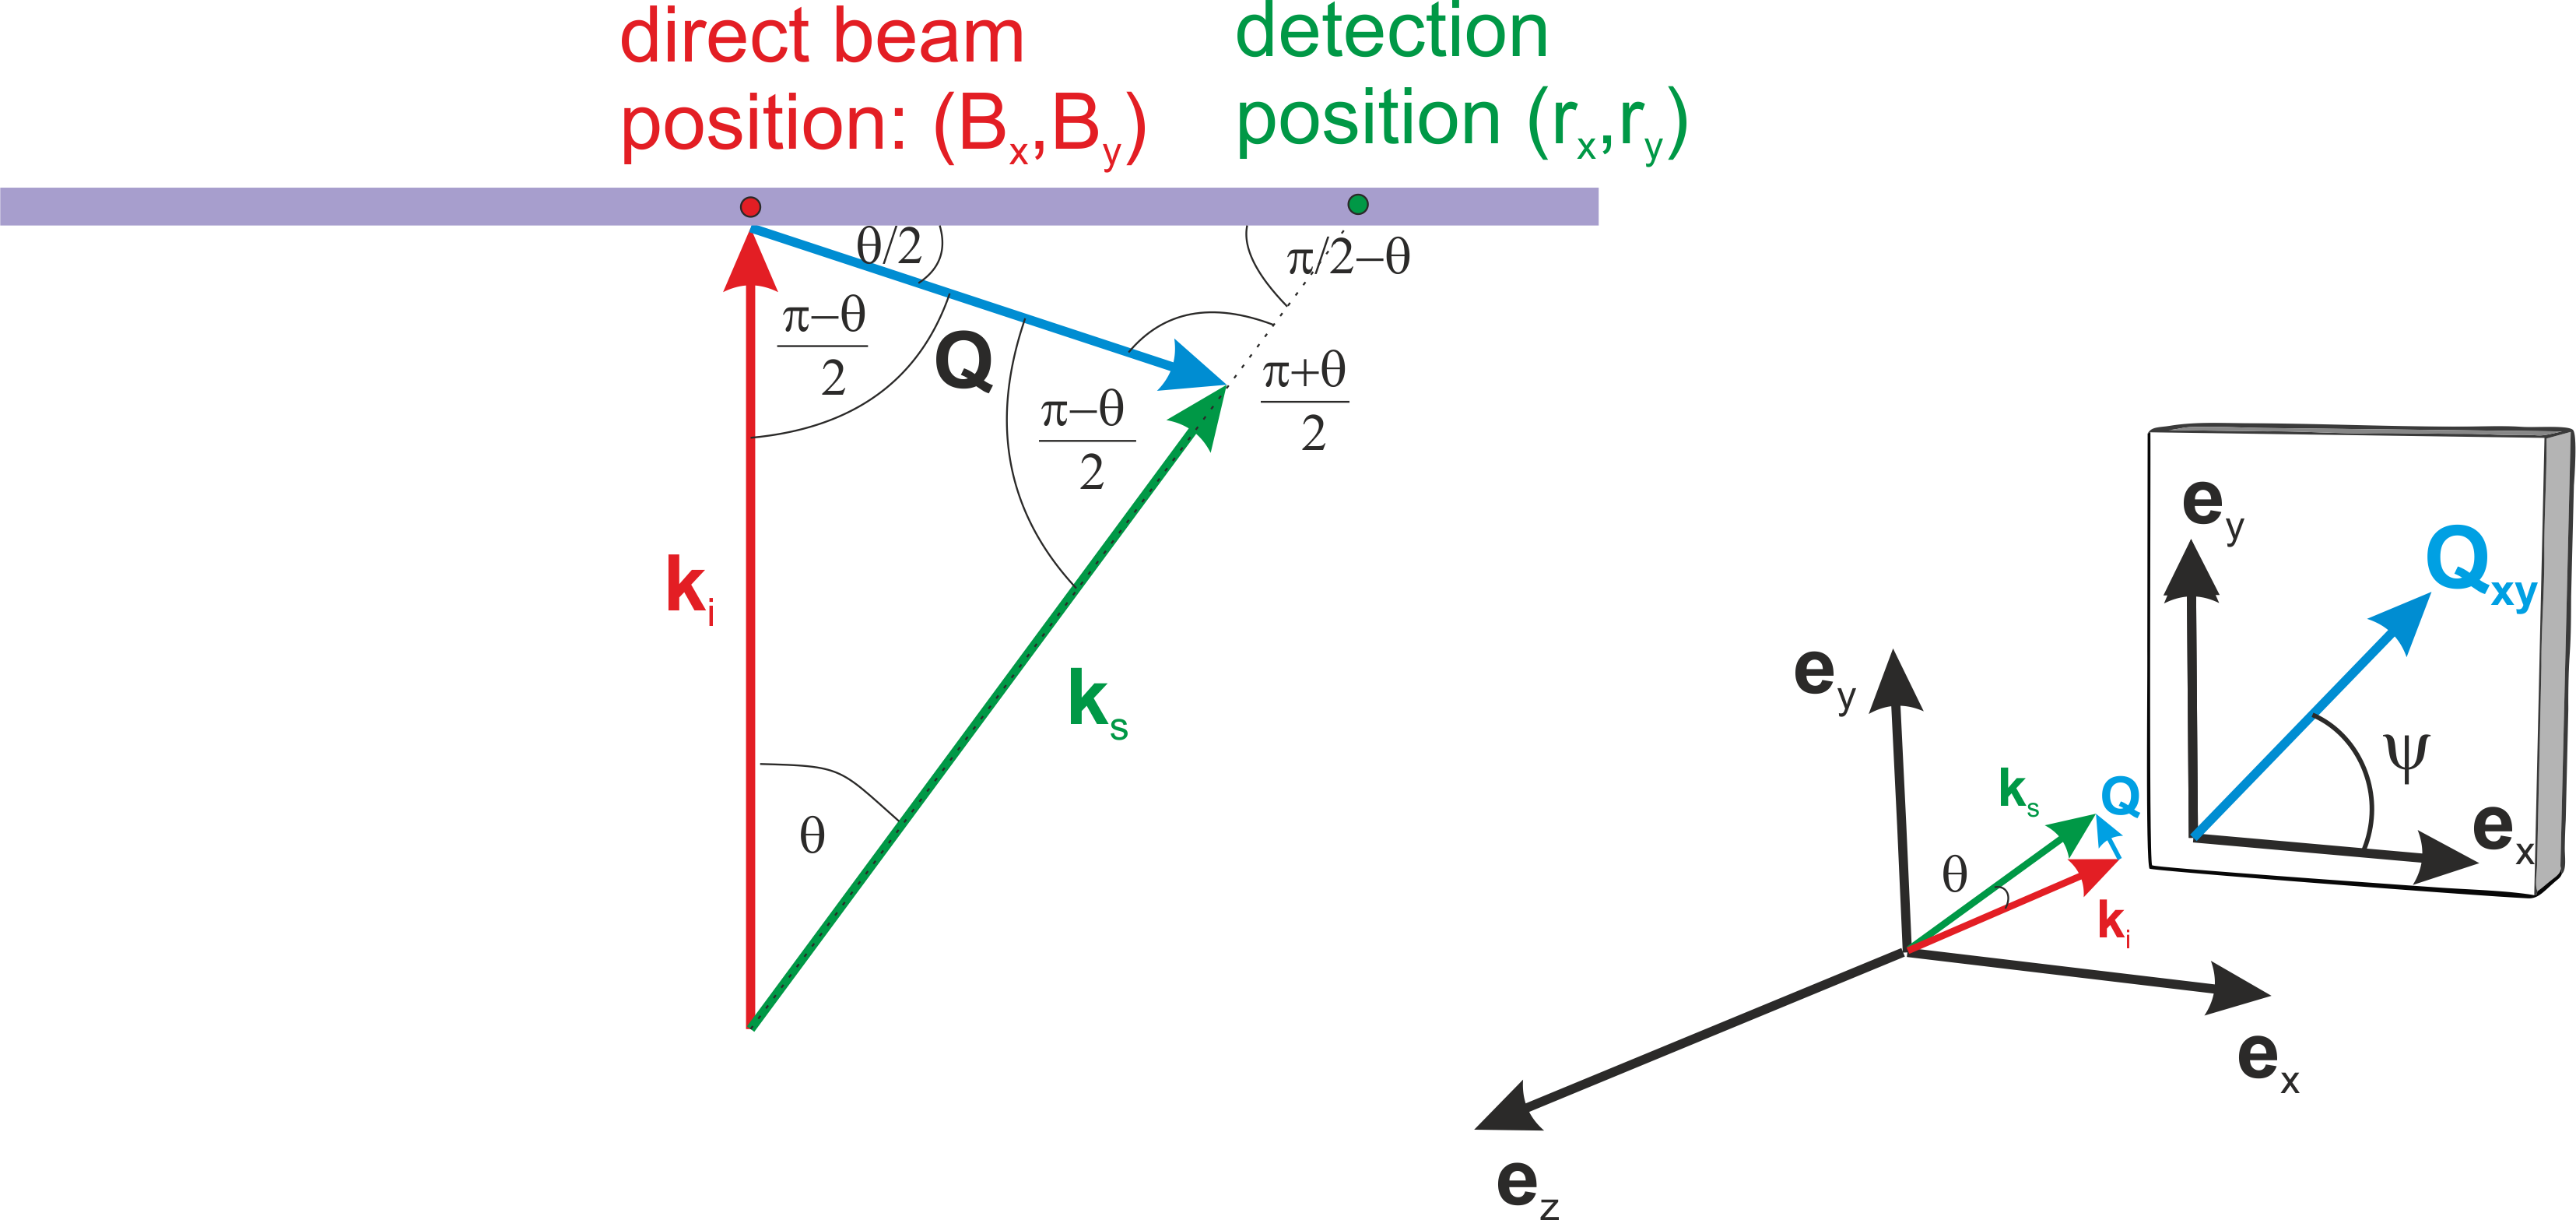
\includegraphics[width=0.85\textwidth]{osp_coord_system.png}
\end{center}
\caption{The scattering vector in polar coordinates coordination system with respect to a laboratory-fixed coordinate system based on the three orthogonal unit vectors ($\mathbf{e}_x$, $\mathbf{e}_y$, $\mathbf{e}_z$). They are arranged such that the x-direction coincides with the x-direction of the detector, and the y-direction coincides with the y-direction of the detector. The direction of the incoming neutron beam is chosen to be $-\mathbf{e}_z$. } \label{fig:opsCoordSys}
\end{figure}

\begin{align}
\mathbf{k}_i &=
    \left(
        \begin{array}{c}
                  k_{i,x} \\
                  k_{i,y} \\
                  k_{i,z}
        \end{array}
    \right)
    = \frac{2\pi}{\lambda}
    \left(
        \begin{array}{c}
                  0\\
                  0 \\
                  -1
        \end{array}
    \right) \\
\mathbf{k}_s &=
    \left(
        \begin{array}{c}
                  k_{i,x} \\
                  k_{i,y} \\
                  k_{i,z}
        \end{array}
    \right)
    = \frac{2\pi}{\lambda}
    \left(
        \begin{array}{c}
                  \cos(\psi) \sin(\theta)\\
                  \sin(\psi) \sin(\theta) \\
                  -\cos(\theta)
        \end{array}
    \right) \\
\mathbf{Q} &= \mathbf{k}_s - \mathbf{k}_i =
    \left(
        \begin{array}{c}
                  Q_{x} \\
                  Q_{y} \\
                  Q_{z}
        \end{array}
    \right)
    = \frac{2\pi}{\lambda}
    \left(
        \begin{array}{c}
                  \cos(\psi) \sin(\theta)\\
                  \sin(\psi) \sin(\theta) \\
                  1-\cos(\theta)
        \end{array}
    \right)
\end{align}


%%%%%%%%%%%%%%%%%%%%%%%%%%%%%%%%%%%%%%%%%%%%%%%%%%%%%%%%%%%%%%%%%%%%%%

\clearpage
\section{Multi Lamellar Structures}

Multi-lamellar structures belong to the family of one dimensional structure factors. In practice the dimension of the structures in the direction of ordering is much smaller than perpendicular to it and it also has a random orientation, i.e. one can perform a powder average. For those structures the scattering function can be factorized \cite{Porod1948,Hosemann1962,Guinier1963,Zhang1994,Lemmich1996,Pabst2000,Pabst2003,Fruhwirth2004} in a cross-section term in the direction of the ordering and a shape factor for the long dimension.

\subsection{Multi-Lamellar Structures, perfect finite stack} \hspace{1pt}\\

\begin{figure}[htb]
\begin{center}
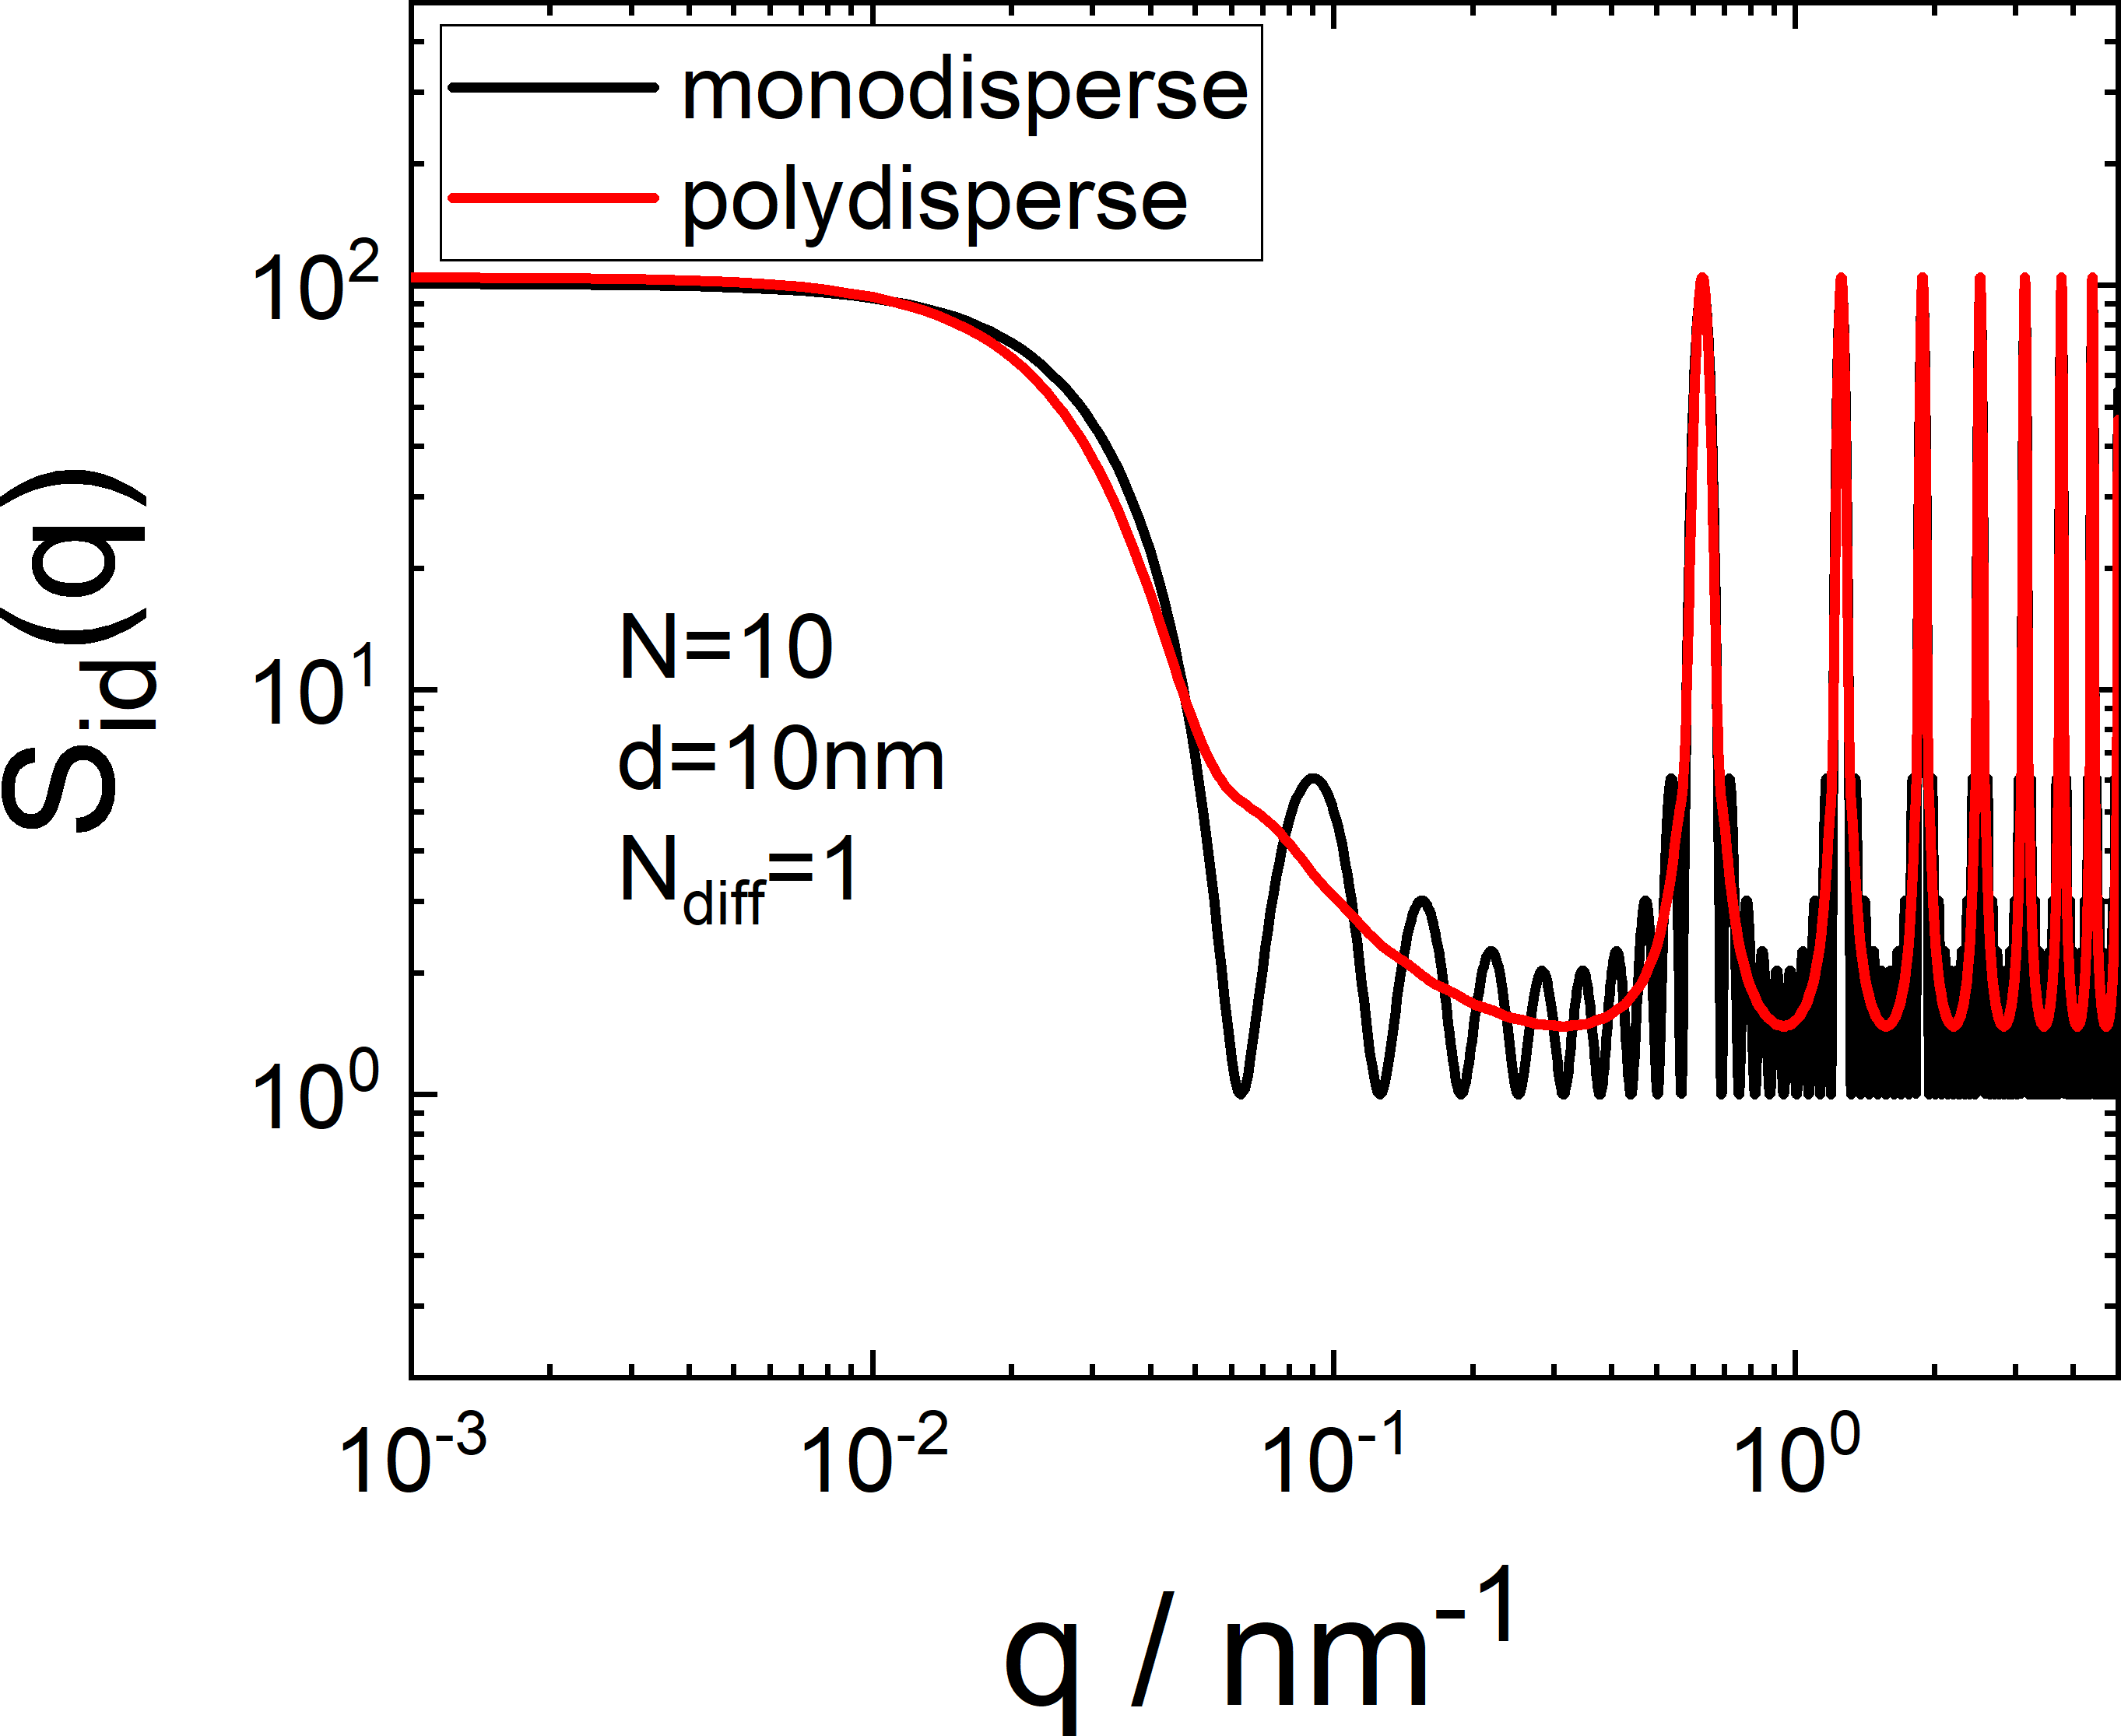
\includegraphics[width=0.7\textwidth]{../images/structure_factor/Lamellar/IDLamellar.png}
\end{center}
\caption{Perfectly ordered lamellar structures with and without a size distribution.}
\label{fig:PerfectOrderSQ}
\end{figure}

If the lamellar structures are perfectly arranged in a one-dimensional lattice with a lattice distance $d$ its structure factor is given by
\begin{align}
  S_{N_k,\mathrm{id}}(q) &= N_k+2\sum_{k=1}^{N_k-1} (N_k-k)\cos(kqd) \label{eq:PerfectFiniteStackMonoSum} +N_\mathrm{diff}\\
       & = \frac{\sin^2\left(\frac12 N_kqd\right)}{\sin^2\left(\frac12 qd\right)} +N_\mathrm{diff}
\end{align}
The above formula is defined for integer values of $N_k$ larger or equal 1. For non-integer values of $N_k$ a mixture between $\lfloor N_k\rfloor$ and $\lfloor N_k\rfloor+1$ is assumed where $\lfloor N_k \rfloor$ denotes the greatest integer less than or equal to $N_k$ (\texttt{\texttt{floor}}-function). We finally get
\begin{align} \label{eq:continuesSQid}
S_\mathrm{id}(q,N_k) &= (1-w)S_{\lfloor N_k\rfloor,\mathrm{id}}(q) + w S_{\lfloor N_k\rfloor+1,\mathrm{id}}(q)
\end{align}
with $w=N_k-\lfloor N_k\rfloor$. This is a classical result for diffraction of perfect ordered limited sized domains.
The Bragg peaks are centered around $q_h=2\pi h/d$, where $h$ denotes
the diffraction order. The width of the peaks are only dependent on the domain size $N_k$.

The structure factors $S_\text{k,id}(q)$ with low, but fixed
stacking numbers $N_k$ show oscillations at low $q$ (as can be seen in
Fig. \ref{fig:PerfectOrderSQ}), but no such oscillations are found in
experimental data. This can be understood as the consequence of
polydispersity in the number of the different stacks. In order to
eliminate these artifacts from strictly monodisperse systems, we use
a `polydisperse' structure factor, i.e. we use an average of a
series of structure factors with varying numbers of bilayers
\cite{Fruhwirth2004}. The analytical form of the distribution is not
known a priori. We use a Gaussian distribution approximated by a
discrete series The standard deviation $\sigma$ for the
Gaussian-weighted distribution is chosen as
\begin{align}
\sigma =
\begin{cases}
\sqrt{N} & \text{for} N\geq 5 \text{,} \\
0.5(N-1) & \text{for} N< 5
\end{cases}
\end{align}
Therefore, $N$ must be greater or equal to 2, which is a
reasonable restriction for multilamellar stacks of bilayers. In
the range of $N \pm 2\sigma$, structure factors are weighted by
\begin{align}
x_k(N_k) & = \frac{1}{\sigma\sqrt{2\pi}} \exp\left[
-\frac{(N_k-N)^2}{2\sigma^2}\right]
\end{align}
where $N$ is the mean number of stacks and $N_k$
is one of the  bilayers in the range $N\pm 2\sigma$. This
polydispersity model does not introduce new free parameters and is
symmetrical around the mean $N$. Due to the continues definition in eq.\ \ref{eq:continuesSQid} we therefore can write the polydispersity effect both as a sum or an integral.
\begin{align}
  S_\mathrm{sd,id}(q) & = \sum_{N_k=N-2\sigma}^{N+2\sigma} x_k(N_k) S_\mathrm{id}(q,N_k) \label{eq:PerfectFiniteStackPolySum} \\
   & = \int_{N-2\sigma}^{N+2\sigma} x_k(N_k) S_\mathrm{id}(q,N_k) \mathrm{d}N_k
  \label{eq:PerfectFiniteStackPolyInt}
\end{align}
\SASfit supplies the original formula eq.\ \ref{eq:PerfectFiniteStackMonoSum} as  \texttt{PerfectFiniteStack} and the smoothed version by introducing some polydispersity in the stacking number according to eq.\ \ref{eq:PerfectFiniteStackPolySum} as \texttt{PerfectFiniteStack (polydisp.,sum)} and \ref{eq:PerfectFiniteStackPolyInt} as \texttt{PerfectFiniteStack (polydisp.,int)}.

\vspace{5mm}

\noindent
\uline{Input Parameters for the models \texttt{PerfectFiniteStack}, \texttt{PerfectFiniteStack} \texttt{(polydisp.,sum)}, and \texttt{PerfectFiniteStack (polydisp.,int)}:}
\begin{description}
\item[\texttt{N}] mean number of stacks $N$
\item[\texttt{d}] stacking separation $d$
\item[\texttt{dummy}]  not used
\item[\texttt{Nu}] number of uncorrelated scattering bilayers $N_\text{diff}$
\end{description}

\noindent\uline{Note:}
\begin{itemize}
\item This structure factor is intended to be used with the \texttt{monodisperse approximation}.
\end{itemize}


\subsection{Multi-Lamellar Structures, Thermal Disorder} \hspace{1pt}\\

\begin{figure}[htb]
\begin{center}
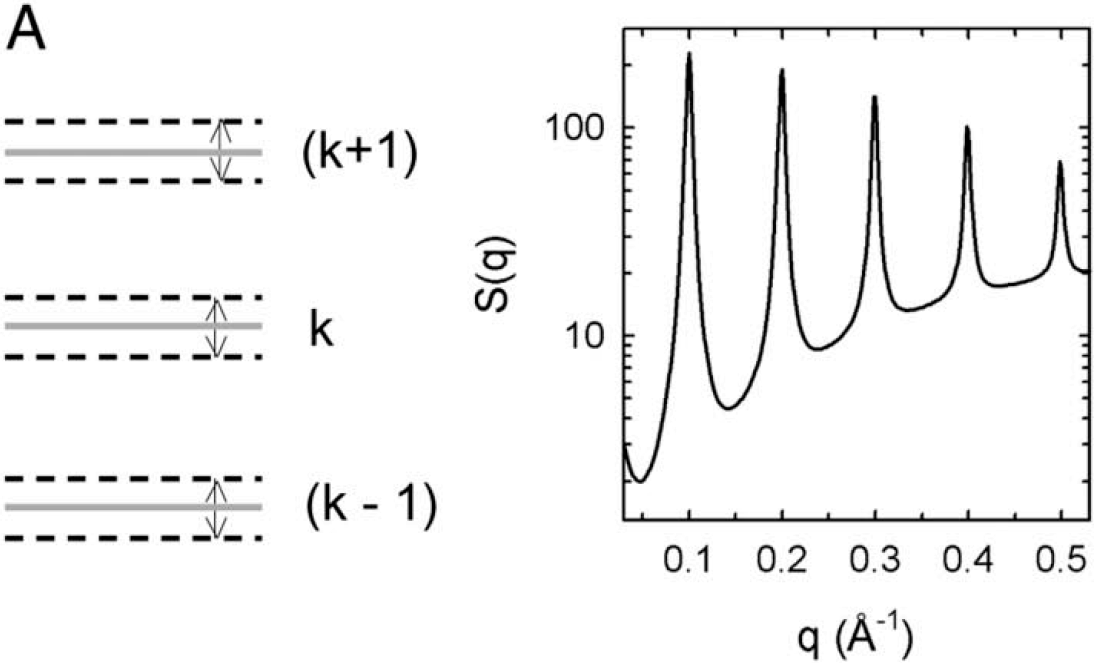
\includegraphics[width=0.7\textwidth]{ThermalDisorderSQ.png}
\end{center}
\caption{Thermal disorder, considering fluctuations of flat layers
around well defined and evenly spaced equilibrium positions.}
\label{ThermalDisorderSQ}
\end{figure}

The first type describes thermal disorder (TD) caused by small
fluctuations of the bilayers around well defined mean layer
positions of equal separation (Fig. \ref{ThermalDisorderSQ}) \cite{Pabst2003,Fruhwirth2004}. In
such a crystal lattice the long-range order is preserved and the
structure factor for a single domain of size $L = Nd$ is identical
to that of a perfect finite crystal multiplied by the well known
Debye-Waller temperature factor, where $\Delta = \left<
(d_k-d)^2\right>$ denotes the mean square fluctuations of the
bilayers. As shown in Fig. \ref{ThermalDisorderSQ},
$S_\text{TD}(Q)$ is characterized by a set of Bragg peaks of equal
width, the diffraction order amplitudes of which decrease
exponentially with the Debye-Waller factor. The lost intensity is
found as a diffuse background scattering, which increases to the
limit of $N$ for large $q$.
For this model and with a lattice distance $d$ and fixed number $N_k$  of layers per stack the structure factor is given by
\begin{align} \label{eq:TDMonoSum}
S_{N_k,\mathrm{TD}}(q) & = \left( N_k + 2 e^{-\frac{q^2\Delta^2}{2}} \sum_{k=1}^{N_k-1} (N_k-k) \cos(kqd) \right) +N_\mathrm{diff}\\
&= N_k \left(1-e^{-\frac{q^2\Delta^2}{2}}\right)+e^{-\frac{q^2\Delta^2}{2}}\left(S_{N_k,\mathrm{id}}(q)-N_\mathrm{diff}\right)+N_\mathrm{diff}
\end{align}
$N_\text{diff}$ accounts for an additional
diffuse background, due to a number of uncorrelated
scattering bilayers in $S_\text{TD}(q,N,d,\Delta,N_\text{diff})$,
which is not included in the TD theory.
Its origin is attributed to bilayers with strong lattice defects or
unilamellar vesicles, which display neither short-range nor
(quasi-) long-range order.
The above formula is defined for integer values of $N_k$ larger or equal 1. For non-integer values of $N_k$ a mixture between $\lfloor N_k\rfloor$ and $\lfloor N_k\rfloor+1$ is assumed where $\lfloor N_k \rfloor$ denotes the greatest integer less than or equal to $N_k$ (\texttt{\texttt{floor}}-function). We finally get
\begin{align} \label{eq:continuesSQTD}
S_\mathrm{TD}(q,N_k) &= (1-w)S_{\lfloor N_k\rfloor,\mathrm{TD}}(q) + w S_{\lfloor N_k\rfloor+1,\mathrm{TD}}(q)
\end{align}
with $w=N_k-\lfloor N_k\rfloor$.
The Bragg peaks are centered around $q_h=2\pi h/d$, where $h$ denotes
the diffraction order.



\begin{figure}[htb]
\begin{center}
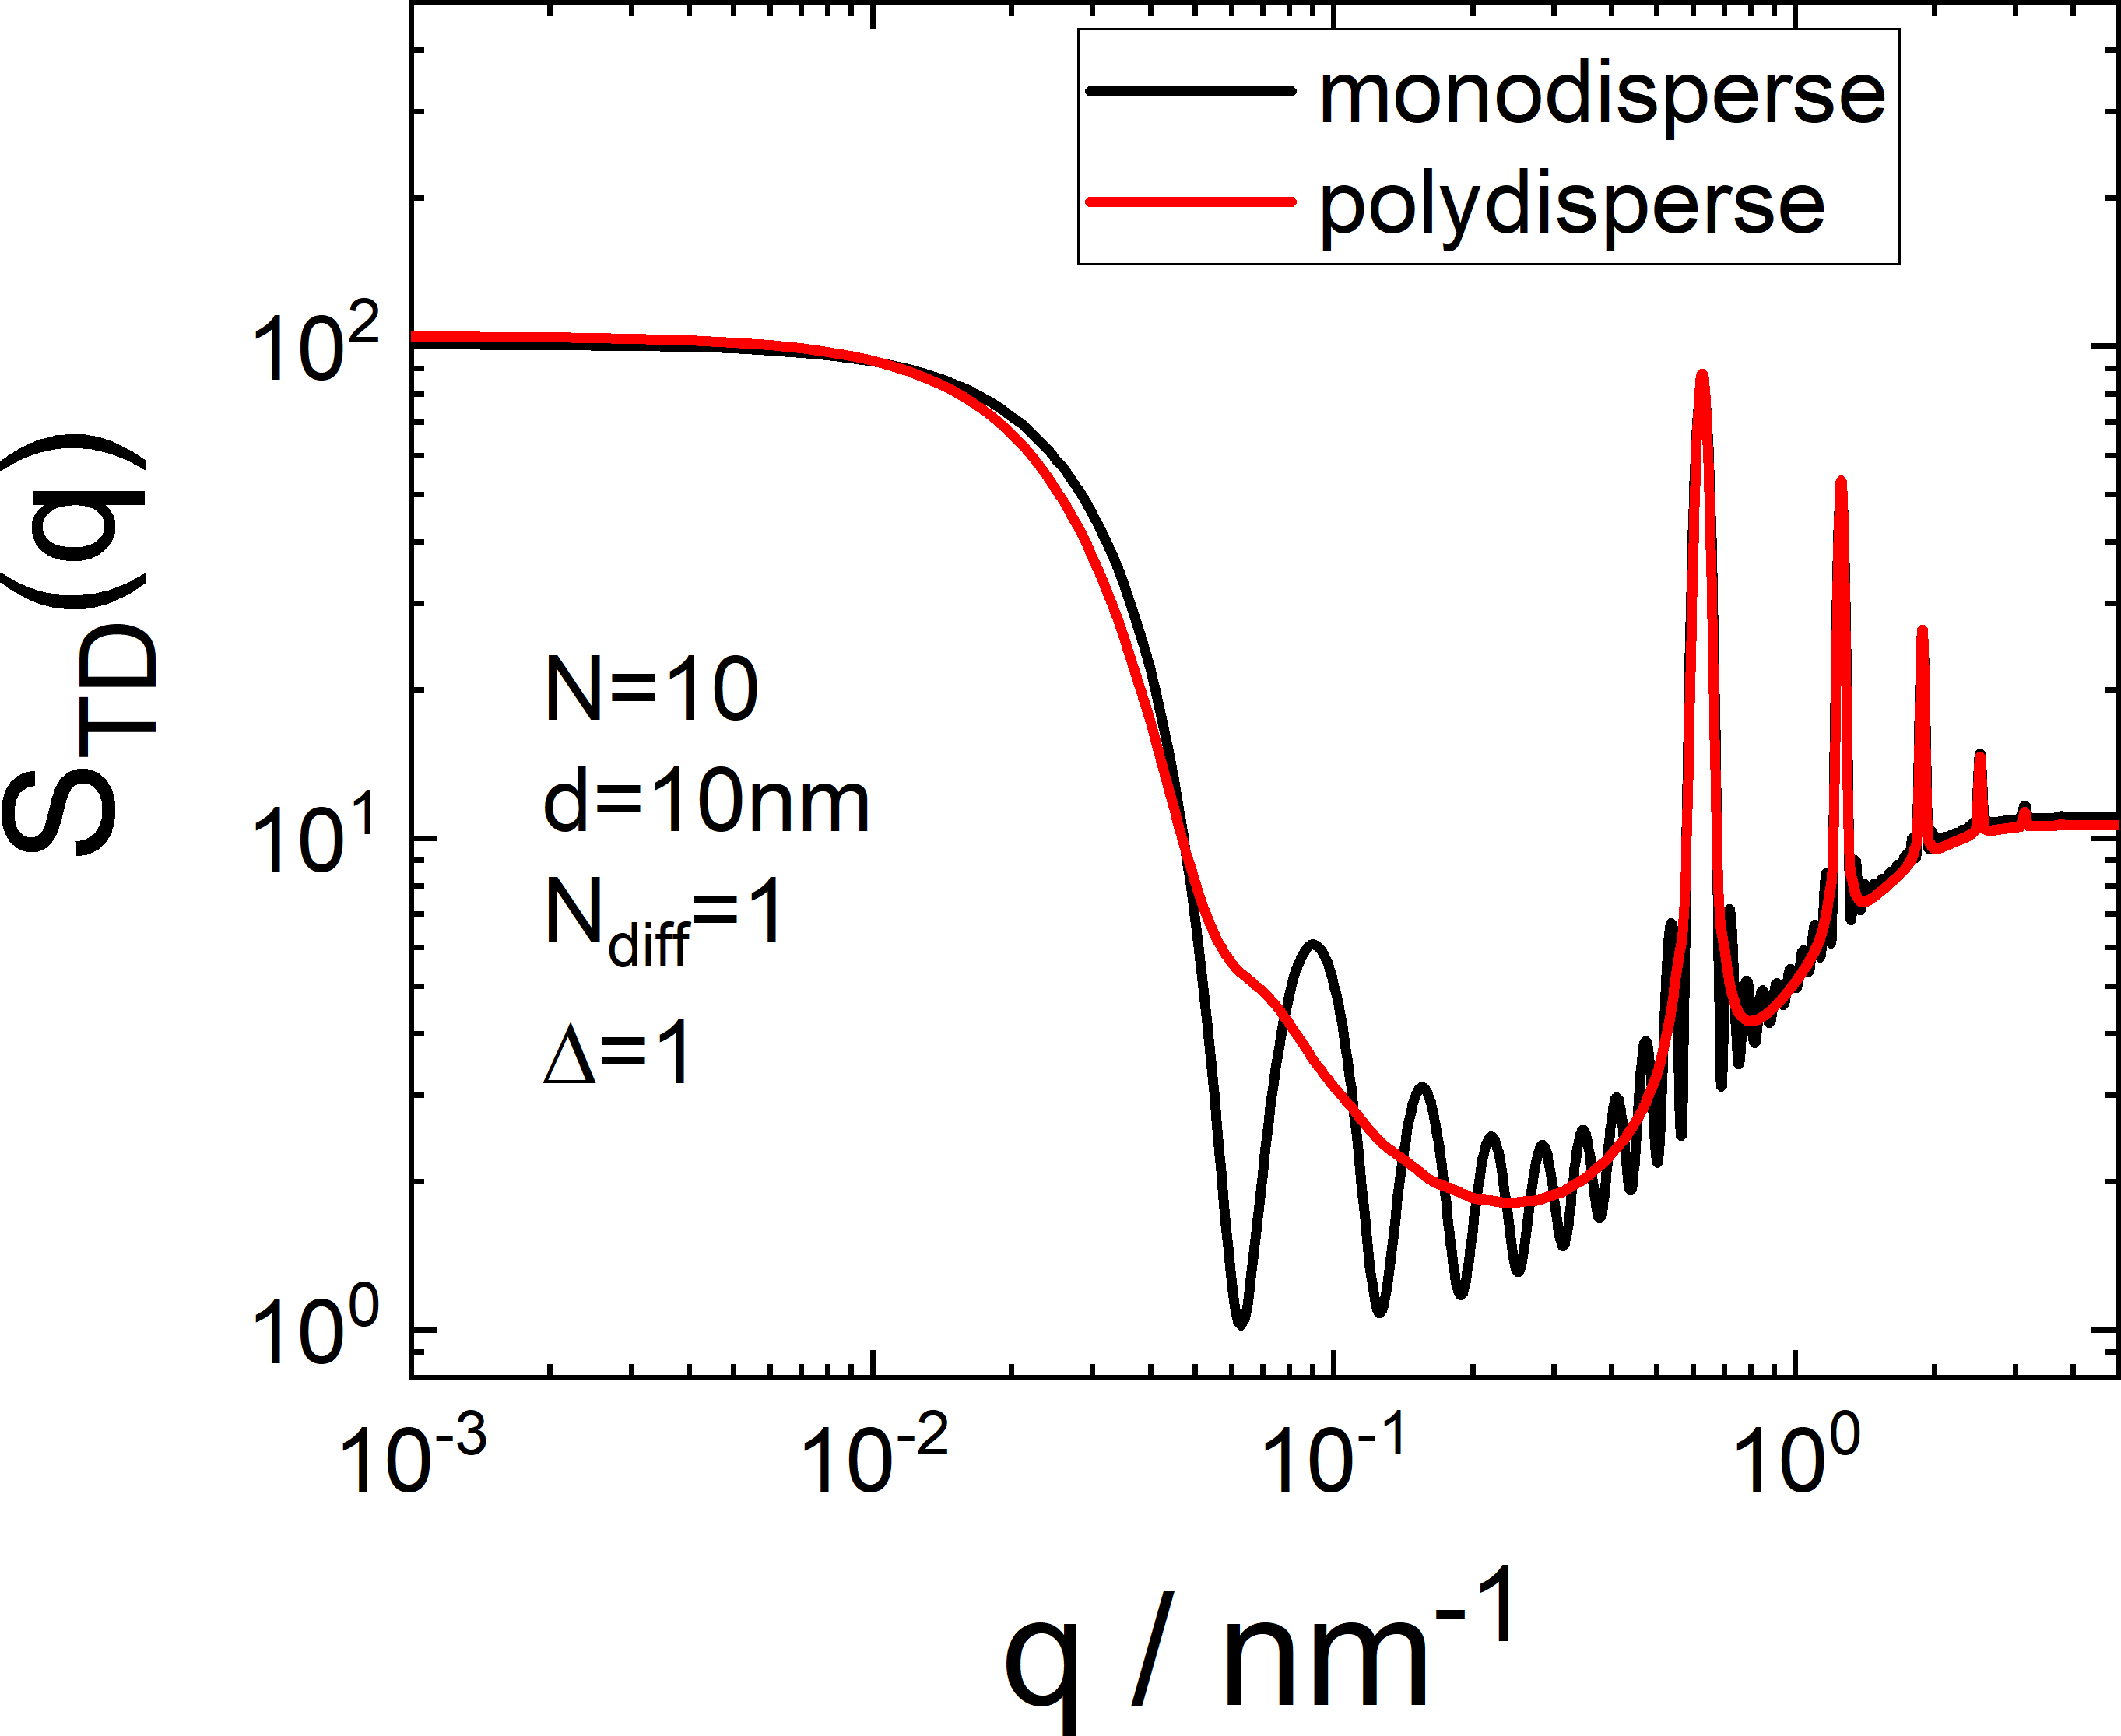
\includegraphics[width=0.65\textwidth]{../images/structure_factor/Lamellar/TDLamellar.png}
\end{center}
\caption{Structure factor of multi-lamellar structures with thermal disorder. }
\label{fig:TDLamellar}
\end{figure}

The structure factors $S_{N_k,\mathrm{TD}}(q)$ with low, but fixed
stacking numbers $N_k$ show oscillations at low $q$ (as can be seen in
Fig. \ref{ThermalDisorderSQ}), but no such oscillations are found in
experimental data. This can be understood as the consequence of
polydispersity in the size of the different stacks. In order to
eliminate these artifacts from strictly monodisperse systems, we use
a `polydisperse' structure factor, i.e. we use an average of a
series of structure factors with varying numbers of bilayers
\cite{Fruhwirth2004}. The analytical form of the distribution is not
known a priori. We use a Gaussian distribution approximated by a
discrete series The standard deviation $\sigma$ for the
Gaussian-weighted distribution is chosen as
\begin{align}
\sigma =
\begin{cases}
\sqrt{N} & \text{for} N\geq 5 \text{,} \\
0.5(N-1) & \text{for} N< 5
\end{cases}
\end{align}
Therefore, $N$ must be greater or equal to 2, which is a
reasonable restriction for multilamellar stacks of bilayers. In
the range of $N \pm 2\sigma$, structure factors weighted by
\begin{align}
x_k & = \frac{1}{\sigma\sqrt{2\pi}} \exp\left[
-\frac{(N_k-N)^2}{2\sigma^2}\right]
\end{align}
are calculated, where $N$ is the mean number of stacks and $N_k$
is one of the  bilayers in the range $N\pm 2\sigma$. This
polydispersity model does not introduce new free parameters and is
symmetrical around the mean $N$. Due to the continues definition in eq.\ \ref{eq:continuesSQTD} we therefore can write the polydisperse effect both as a sum or an integral.
\begin{align}
  S_\mathrm{sd,TD}(q) & = \sum_{N_k=N-2\sigma}^{N+2\sigma} x_k(N_k) S_\mathrm{TD}(q,N_k) \label{eq:TDPolySum} \\
                      & = \int_{N-2\sigma}^{N+2\sigma} x_k(N_k) S_\mathrm{TD}(q,N_k) \mathrm{d}N_k \label{eq:TDPolyInt}
\end{align}
\SASfit supplies the original formula eq.\ \ref{eq:TDMonoSum} as  \texttt{ThermalDisorder} and the smoothed version by introducing some polydispersity in the stacking number according to eq.\ \ref{eq:TDPolySum} as \texttt{ThermalDisorder (polydisp.,sum)} and \ref{eq:TDPolyInt} as \texttt{ThermalDisorder (polydisp.,int)}.


\vspace{5mm}

\noindent
\uline{Input Parameters for model \texttt{ThermalDisorder}, \texttt{ThermalDisorder (polydisp.,sum)}, and \texttt{ThermalDisorder (polydisp.,int)}:}
\begin{description}
\item[\texttt{N}] mean number of stacks $N$
\item[\texttt{d}] stacking separation $d$
\item[\texttt{Delta}]  Debye-Waller disorder parameter $\Delta$
\item[\texttt{Nu}]   number of uncorrelated scattering bilayers $N_\text{diff}$
\end{description}

\noindent\uline{Note:}
\begin{itemize}
\item This structure factor is intended to be used with the \texttt{monodisperse approximation}.
\end{itemize}

%%%%%%%%%%%%%%%%%%%%%%%%%%%%%%%%%%%%%%%%%%%%%%%%%%%%%%%%%%%%%%%%%%%%%%%%%%%%%%%%%%%%%%%%%%

\subsection{Multi-Lamellar Structures, Paracrystalline Theory} ~\\

\begin{figure}[htb]
\begin{center}
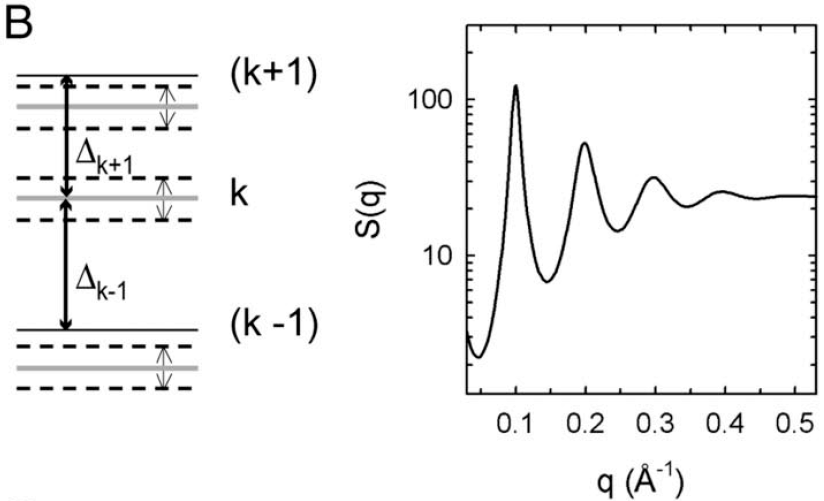
\includegraphics[width=0.7\textwidth]{ParacrystallineTheorySQ.png}
\end{center}
\caption{Stacking disorder as described within paracrystalline
theory (PC) is due to displacements from the mean layer
positions.} \label{ParacrystallineTheorySQ}
\end{figure}


The second type of disorder accounts for the presence of small
variations in the bilayer separations (Fig.
\ref{ParacrystallineTheorySQ}), so-called stacking disorder, and is
described within the paracrystalline theory (PC)
\cite{Hosemann1962,Guinier1963,Blaurock1982,Pabst2003,Fruhwirth2004}. As the position of an
individual fluctuating layer in a paracrystal is determined solely
by its nearestneighbour membranes, the crystalline long-range order
is lost. Still, we are able to observe Bragg-peak scattering due to
the fact that there is quasi long-range order. However, these
quasi-Bragg peaks will display a typical line shape. In the case of
disorder of the second kind, the structure factor derived from
paracrystalline theory is given by \cite{Guinier1963}
\begin{align} \label{eq:PCMonoSum}
S_{N_k,\mathrm{PC}}(q) &= \left( N_k + 2 \sum_{k=1}^{N_k-1} (N_k-k)
\cos(kqd) \exp\left( -\frac{kq^2\Delta^2}{2}\right) \right) +N_\mathrm{diff}%\\
%&= N_k\frac{1- \exp\left(-q^2\Delta^2\right)}{1+ \exp\left(-q^2\Delta^2\right)-2\cos(qd) \exp\left(-\frac12 q^2\Delta^2\right)}
\end{align}
$N_\text{diff}$ accounts for an additional
diffuse background, due to a number of uncorrelated
scattering bilayers in $S_\text{PC}(q,N,d,\Delta,N_\text{diff})$,
which is not included in the paracrystalline theory.
Its origin is attributed to bilayers with strong lattice defects or
unilamellar vesicles, which display neither short-range nor
(quasi-) long-range order.
The above formula is defined for integer values of $N_k$ larger or equal 1. For non-integer values of $N_k$ a mixture between $\lfloor N_k\rfloor$ and $\lfloor N_k\rfloor+1$ is assumed where $\lfloor N_k \rfloor$ denotes the greatest integer less than or equal to $N_k$ (\texttt{\texttt{floor}}-function). We finally get
\begin{align} \label{eq:continuesSQPC}
S_\mathrm{PC}(q,N_k) &= (1-w)S_{\lfloor N_k\rfloor,\mathrm{PC}}(q) + w S_{\lfloor N_k\rfloor+1,\mathrm{PC}}(q)
\end{align}
with $w=N_k-\lfloor N_k\rfloor$.
The Bragg peaks are centered around $q_h=2\pi h/d$, where $h$ denotes
the diffraction order.

Fig. \ref{ParacrystallineTheorySQ} shows that the quasi-Bragg peak
intensity decreases for $S_\text{PC}(q)$, as in the previous case of
thermal disorder. However, the decrease in peak height is also
accompanied by a progressive broadening proportional to the square
of the diffraction order $h$ \cite{Schwartz1975}. The line shape of
the tails is essentially Lorentzian with
$$S_\text{k,PC}(q) \propto (q - q_h)^2,$$
where $q_h$ is the position of the $h^\text{th}$ diffraction order
in $q$ space. Again, the loss in intensity shows up as diffuse
background scattering, which is stronger than from pure thermal
disorder.


The structure factors $S_\text{k,PT}(q)$ with low, but fixed
stacking numbers $N$ show oscillations at low $q$ (as can be seen in
Fig. \ref{ParacrystallineTheorySQ}), but no such oscillations are
found in experimental data. This can be understood as the
consequence of polydispersity in the size of the different stacks.
In order to eliminate these artifacts from strictly monodisperse
systems, we use a `polydisperse' structure factor, i.e. we use an
average of a series of structure factors with varying numbers of
bilayers \cite{Fruhwirth2004}. The analytical form of the
distribution is not known a priori. We use a Gaussian distribution
approximated by a discrete series The standard deviation $\sigma$
for the Gaussian-weighted distribution is chosen as
\begin{align}
\sigma =
\begin{cases}
\sqrt{N} & \text{for} N\geq 5 \text{,} \\
0.5(N-1) & \text{for} N< 5
\end{cases}
\end{align}
Therefore, $N$ must be greater or equal to 2, which is a
reasonable restriction for multilamellar stacks of bilayers. In
the range of $N \pm 2\sigma$, structure factors weighted by
\begin{align}
x_k & = \frac{1}{\sigma\sqrt{2\pi}} \exp\left[
-\frac{(N_k-N)^2}{2\sigma^2}\right]
\end{align}
are calculated, where $N$ is the mean number of stacks and $N_k$
is one of the  bilayers in the range $N\pm 2\sigma$. This
polydispersity model does not introduce new free parameters and is
symmetrical around the mean $N$.
 Due to the continues definition in eq.\ \ref{eq:continuesSQPC} we therefore can write the polydisperse effect both as a sum or an integral.
\begin{align}
  S_\mathrm{sd,PC}(q) & = \sum_{N_k=N-2\sigma}^{N+2\sigma} x_k(N_k) S_\mathrm{PC}(q,N_k) \label{eq:PCPolySum} \\
                      & = \int_{N-2\sigma}^{N+2\sigma} x_k(N_k) S_\mathrm{PC}(q,N_k) \mathrm{d}N_k \label{eq:PCPolyInt}
\end{align}
\SASfit supplies the original formula eq.\ \ref{eq:PCMonoSum} as  \texttt{Paracrystalline} and the smoothed version by introducing some polydispersity in the stacking number according to eq.\ \ref{eq:PCPolySum} as \texttt{Paracrystalline (polydisp.,sum)} and \ref{eq:PCPolyInt} as \texttt{Paracrystalline (polydisp.,int)}.


\begin{figure}[htb]
\begin{center}
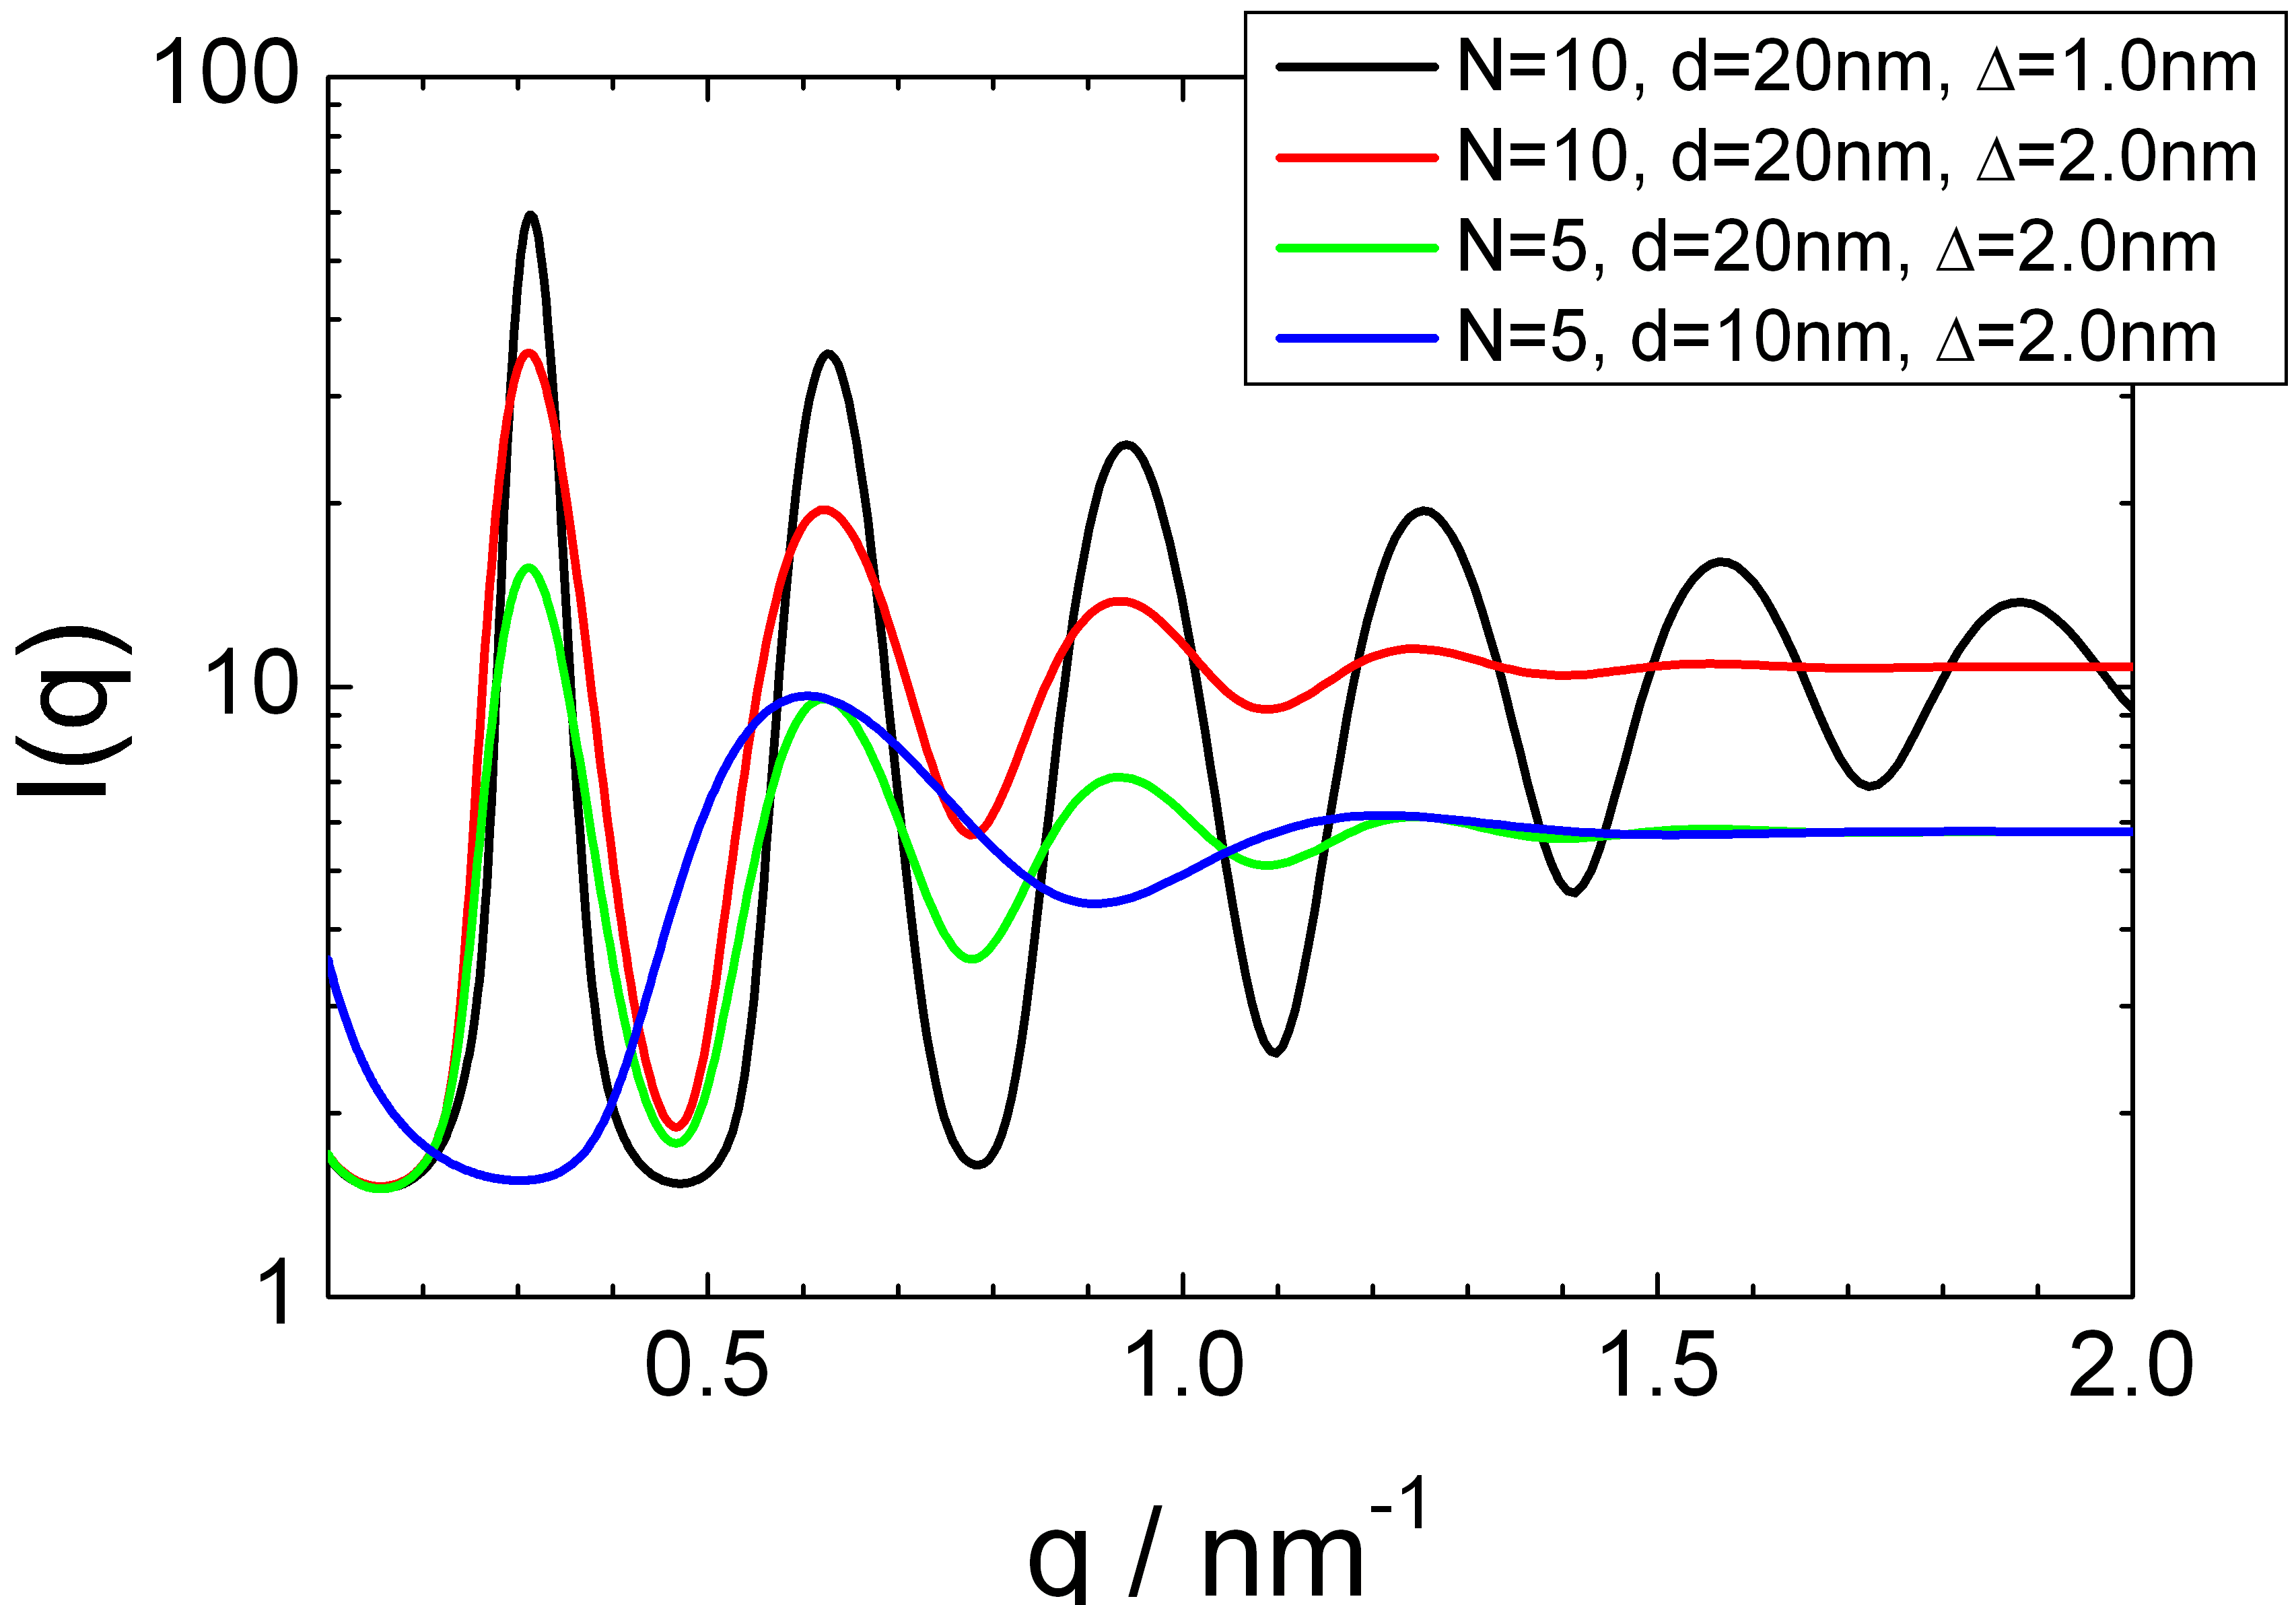
\includegraphics[width=0.65\textwidth]{../images/structure_factor/Lamellar/PCLamellar.png}
\end{center}
\caption{Structure factor of multi-lamellar structures with para-crystalline disorder. }
\label{fig:PCLamellar}
\end{figure}

\vspace{5mm}

\noindent
\uline{Input Parameters for model \texttt{Paracrystalline}, \texttt{Paracrystalline (polydisp.,sum)}, and  \texttt{Paracrystalline (polydisp.,int)}:}
\begin{description}
\item[\texttt{N}] mean number of stacks $N$
\item[\texttt{d}] stacking separation $d$
\item[\texttt{Delta}]  stacking disorder parameter $\Delta$
\item[\texttt{Nu}]   number of uncorrelated scattering bilayers $N_\text{diff}$
\end{description}

\noindent\uline{Note:}
\begin{itemize}
\item This structure factor is intended to be used with the \texttt{monodisperse approximation}.
\end{itemize}

%%%%%%%%%%%%%%%%%%%%%%%%%%%%%%%%%%%%%%%%%%%%%%%%%%%%%%%%%%%%%%%%%%%%%%%

\subsection{Multi-Lamellar Structures, Modified Caill\'e Theory} ~\\

\begin{figure}[htb]
\begin{center}
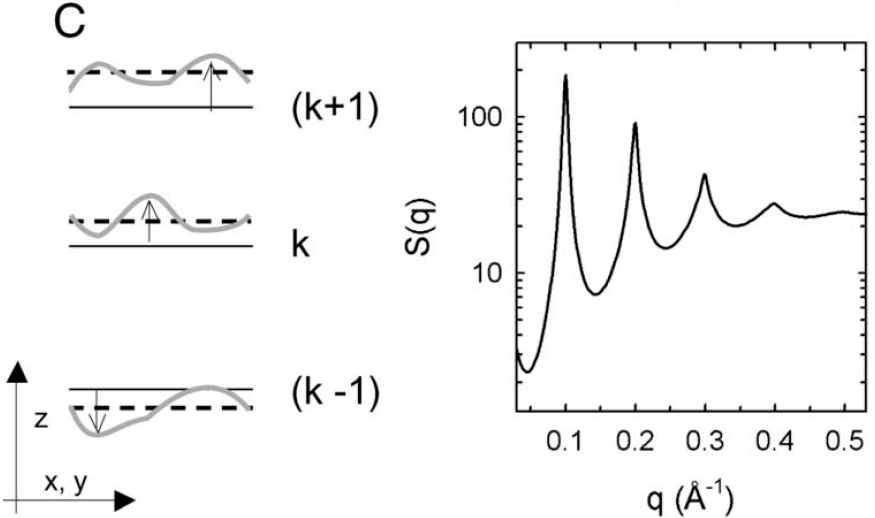
\includegraphics[width=0.7\textwidth]{ModifiedCailleTheorySQ.png}
\end{center}
\caption{Bending fluctuation disorder is a particular feature of
the $L_\alpha$ (smectic A) phase and is caused by bilayer
undulations. The particular shape of the Bragg peaks is given by
the modified Caill\'e theory (MC).}
\label{ModifiedCailleTheorySQ}
\end{figure}

There is another type of disorder when bilayer bending fluctuations
are considered (Fig. \ref{ModifiedCailleTheorySQ}) \cite{Pabst2003,Fruhwirth2004}. Such
fluctuations are particularly pronounced in the fluid $L_\alpha$
phase (equivalent to smectic A). Caill\'e bending fluctuation
disorder is a particular feature of the $L_\alpha$ (smectic A) phase
and is caused by bilayer undulations. The particular shape of the
Bragg peaks is given by the modified Caill\'e theory (MC).
\cite{Caille1972} realized the impact on the structure factor, which
in a modified version \cite{Zhang1994} of the Caill\'e theory
is
\begin{multline} \label{eq:MCMonoSum}
S_{N_k,\mathrm{MC}}(q) = N_\mathrm{diff}+ N_k \\
                        + 2 \sum_{k=1}^{N_k-1} (N_k-k) \cos(kqd) \,
                            e^{ -\left(\frac{d}{2\pi}\right)^2 q^2 \eta_1 \gamma }
                             \, (\pi k)^{-(d/2\pi)^2Q^2\eta_1}
\end{multline}
Here, $\gamma$ is Euler's constant and
\begin{align}
 \eta_1& = \pi k_B T / 2d^2(BK_c)^{1/2}
\end{align}
is the Caill\'e parameter, which is a measure for the bilayer
fluctuations and is inversely proportional to the square root of the
bilayer bending rigidity $K_c$ times the bulk modulus of compression
$B$ (De Gennes \& Prost, 1993). Therefore, a lineshape analysis of
the quasi-Bragg peaks opens an important experimental window on
interbilayer interactions. Further, $K_c$ and $B$ can be decoupled
as demonstrated recently by hydration studies
\cite{Petrache1998,Pabst2003}, or more elegantly by measuring
multibilayers aligned on a solid substrate \cite{Lyatskaya2000}.
$N_\text{diff}$ accounts for an additional diffuse background, due
to a number of uncorrelated scattering bilayers in
$S_{N_k,\mathrm{MC}}(q,d,\eta_1,\gamma, N_\text{diff}) $, which is not
included in the MCT. Its origin is attributed to bilayers with
strong lattice defects or unilamellar vesicles, which display
neither short-range nor (quasi-) long-range order.
The above formula is defined for integer values of $N_k$ larger or equal 1. For non-integer values of $N_k$ a mixture between $\lfloor N_k\rfloor$ and $\lfloor N_k\rfloor+1$ is assumed where $\lfloor N_k \rfloor$ denotes the greatest integer less than or equal to $N_k$ (\texttt{\texttt{floor}}-function). We finally get
\begin{align} \label{eq:continuesSQMC}
S_\mathrm{MC}(q,N_k) &= (1-w)S_{\lfloor N_k\rfloor,\mathrm{MC}}(q) + w S_{\lfloor N_k\rfloor+1,\mathrm{MC}}(q)
\end{align}
with $w=N_k-\lfloor N_k\rfloor$.

Fig. \ref{ModifiedCailleTheorySQ} shows a typical example of
$S_{\mathrm{MC}}(q)$, which is similar to $S_\text{PC}(q)$ with
respect to the progressive decrease in peak height and increase in
peak width, but which differs significantly in line shape as
\begin{align}
S_{\mathrm{MC}}(q) \propto (q-q_h)^{-1+\eta_1 h^2}
\end{align}
for randomly oriented scattering domains \cite{Roux1988,Zhang1994}.


The structure factors $S_{\mathrm{MC}}(q)$ with low, but fixed
stacking numbers $N_k$ show oscillations at low $q$ (as can be seen in
Fig. \ref{ModifiedCailleTheorySQ}), but no such oscillations are
found in experimental data. This can be understood as the
consequence of polydispersity in the size of the different stacks.
In order to eliminate these artifacts from strictly monodisperse
systems, we use a `polydisperse' structure factor, i.e. we use an
average of a series of structure factors with varying numbers of
bilayers \cite{Fruhwirth2004}. The analytical form of the
distribution is not known a priori. We use a Gaussian distribution
approximated by a discrete series The standard deviation $\sigma$
for the Gaussian-weighted distribution is chosen as
\begin{align}
\sigma =
\begin{cases}
\sqrt{N} & \text{for} N\geq 5 \text{,} \\
0.5(N-1) & \text{for} N< 5
\end{cases}
\end{align}
Therefore, $N$ must be greater or equal to 2, which is a
reasonable restriction for multilamellar stacks of bilayers. In
the range of $N \pm 2\sigma$, structure factors weighted by
\begin{align}
x_k & = \frac{1}{\sigma\sqrt{2\pi}} \exp\left[
-\frac{(N_k-N)^2}{2\sigma^2}\right]
\end{align}
are calculated, where $N$ is the mean number of stacks and $N_k$
is one of the  bilayers in the range $N\pm 2\sigma$. This
polydispersity model does not introduce new free parameters and is
symmetrical around the mean $N$.

Due to the continues definition in eq.\ \ref{eq:continuesSQMC} we therefore can write the polydisperse effect both as a sum or an integral.
\begin{align}
  S_\mathrm{sd,MC}(q) & = \sum_{N_k=N-2\sigma}^{N+2\sigma} x_k(N_k) S_\mathrm{MC}(q,N_k) \label{eq:MCPolySum} \\
                      & = \int_{N-2\sigma}^{N+2\sigma} x_k(N_k) S_\mathrm{MC}(q,N_k) \mathrm{d}N_k \label{eq:MCPolyInt}
\end{align}
\SASfit supplies the original formula eq.\ \ref{eq:MCMonoSum} as  \texttt{ModifiedCaille} and the smoothed version by introducing some polydispersity in the stacking number according to eq.\ \ref{eq:MCPolySum} as \texttt{ModifiedCaille (polydisp.,sum)} and \ref{eq:MCPolyInt} as \texttt{ModifiedCaille (polydisp.,int)}.

\begin{figure}[htb]
\begin{center}
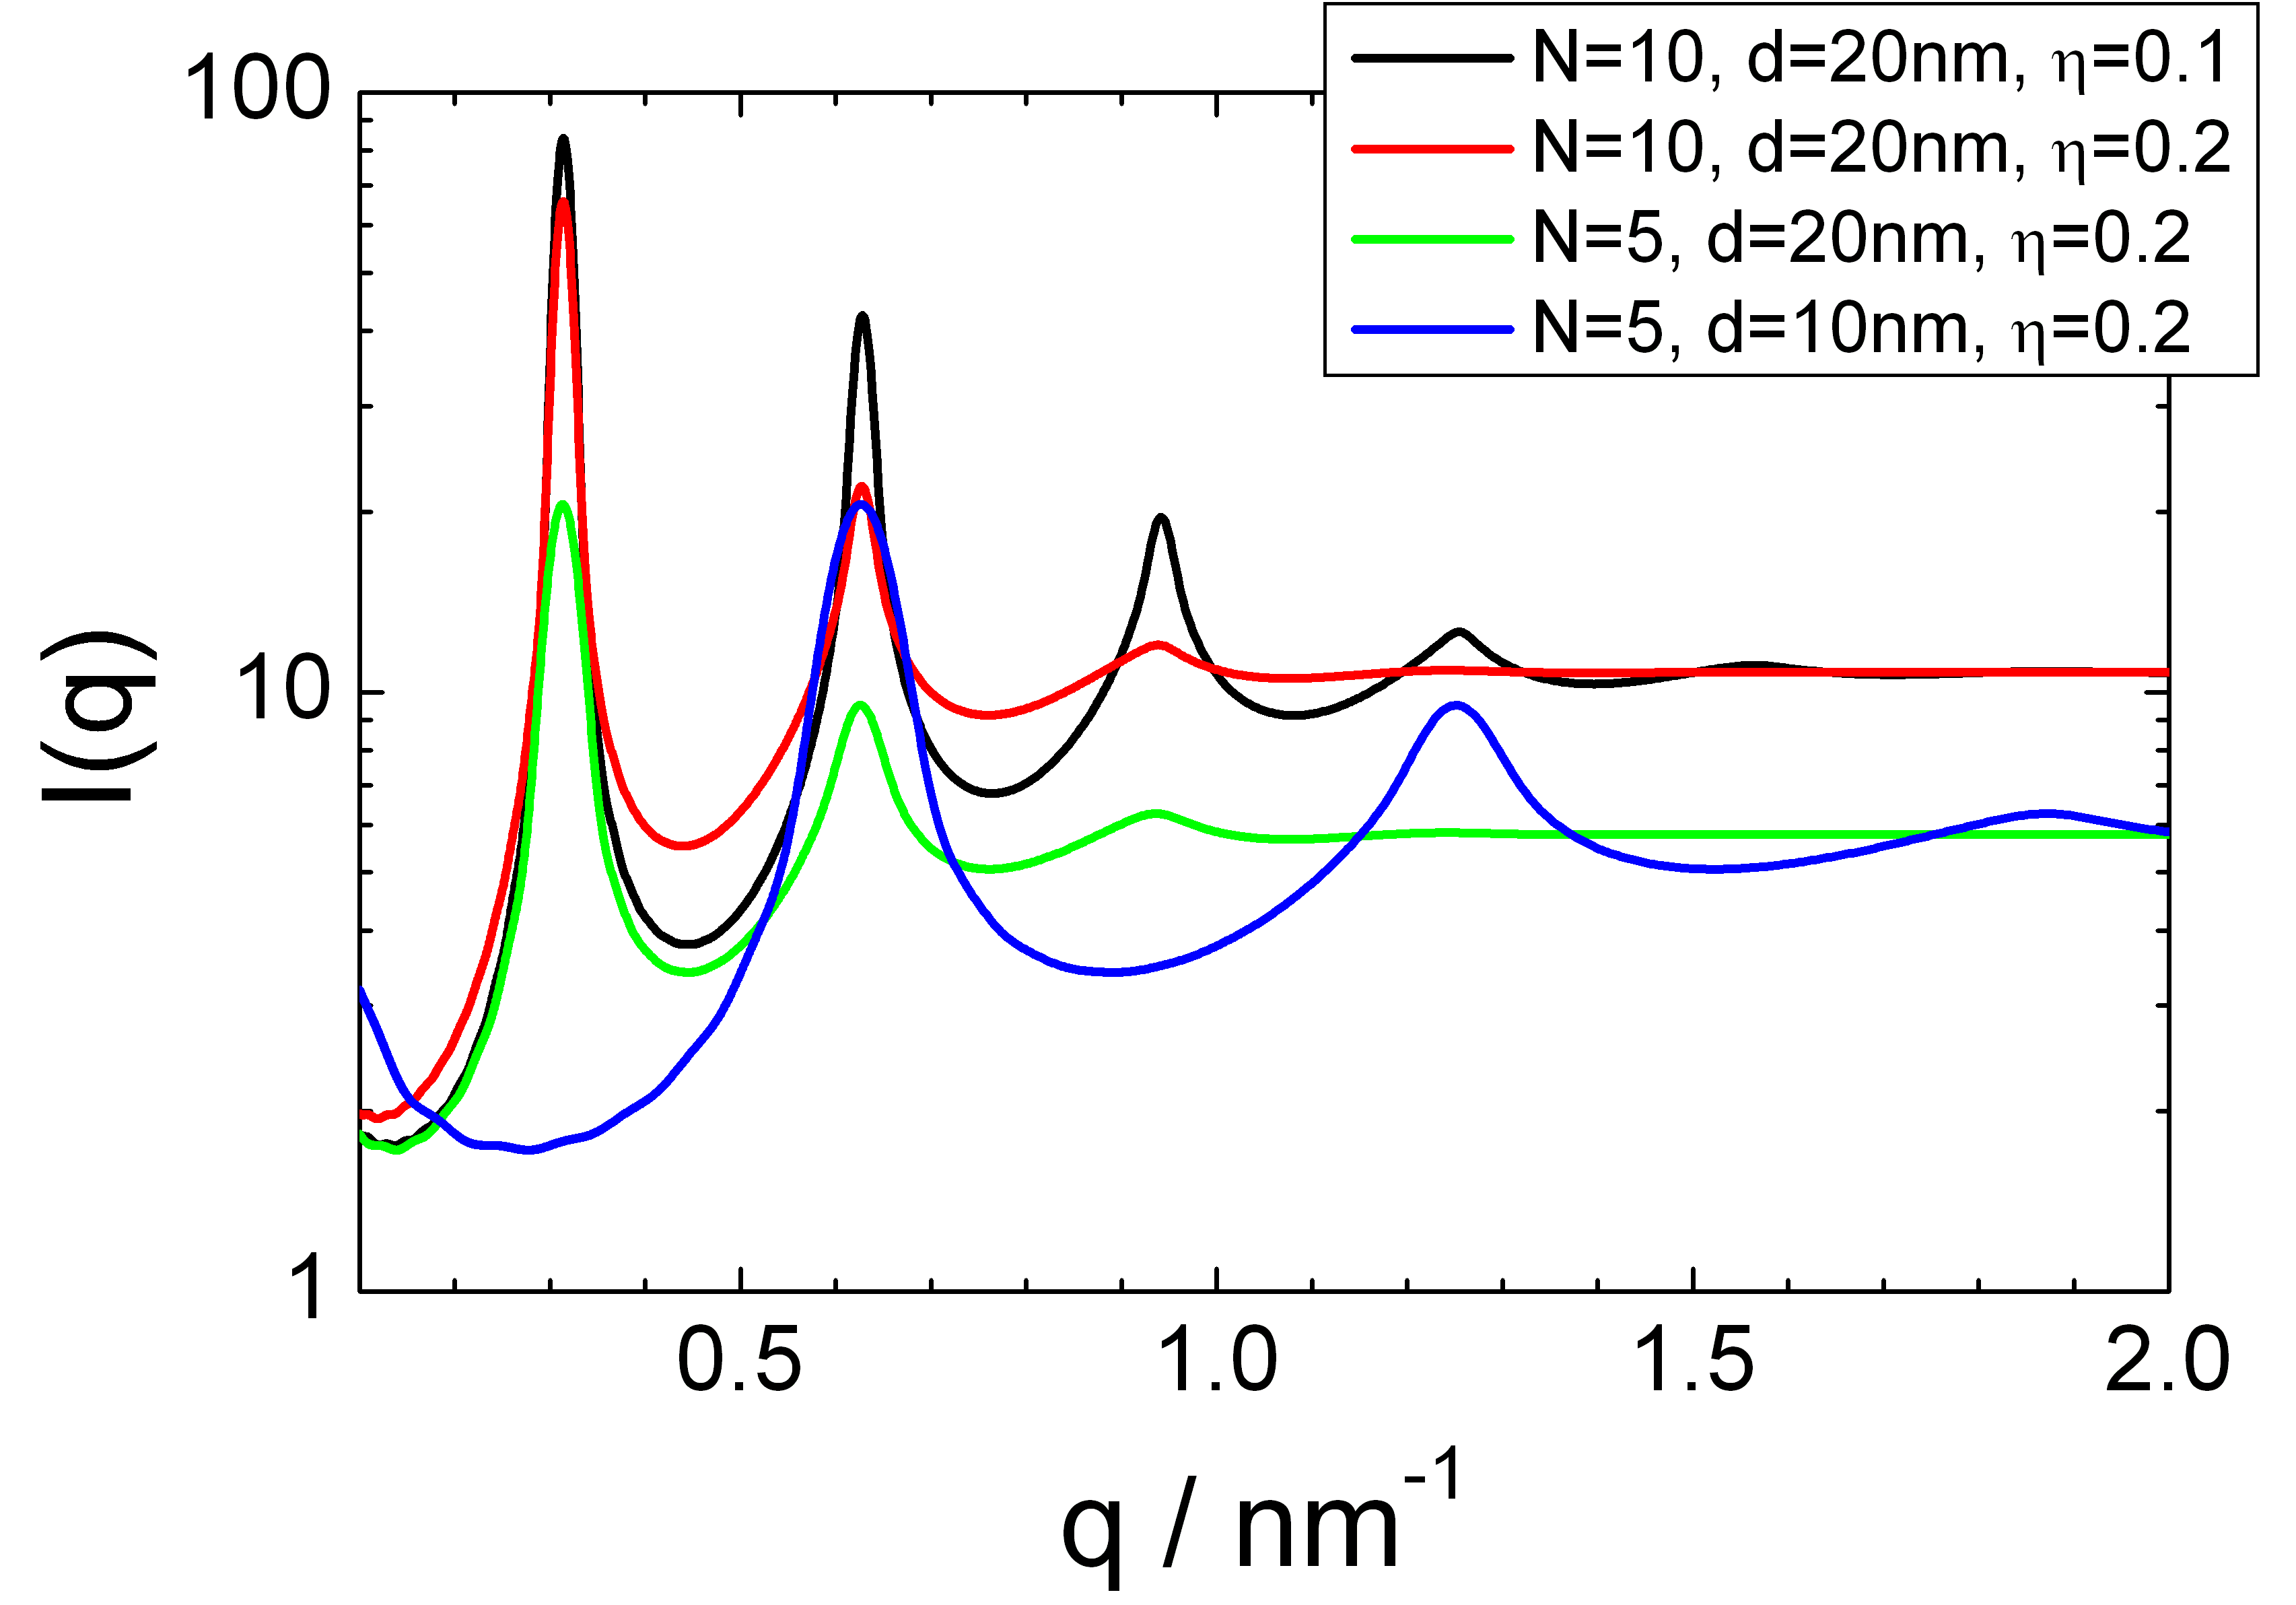
\includegraphics[width=0.65\textwidth]{../images/structure_factor/Lamellar/MCLamellar.png}
\end{center}
\caption{Structure factor of multi-lamellar structures according to the modified Caill\'e theory.}
\label{fig:MCLamellar}
\end{figure}

\vspace{5mm}

\noindent
\uline{Input Parameters for model \texttt{ModifiedCaille}, \texttt{ModifiedCaille (polydisp.,sum)}, and  \texttt{ModifiedCaille (polydisp.,int)}:}
\begin{description}
\item[\texttt{N}] mean number of stacks $N$
\item[\texttt{d}] stacking separation $d$
\item[\texttt{eta}]  the Caill\'e parameter $\eta_1$ is a measure for the bilayer
fluctuations and inversely proportional to the square root of
the bilayer bending rigidity
\item[\texttt{Nu}]   number of uncorrelated scattering bilayers $N_\text{diff}$
\end{description}

\noindent\uline{Note:}
\begin{itemize}
\item This structure factor is intended to be used with the \texttt{monodisperse approximation}.
\end{itemize}

%%%%%%%%%%%%%%%%%%%%%%%%%%%%%%%%%%%%%%%%%%%%%%%%%%%%%%%%%%%%%%%%%%%%%%%%%%%%%%%%%%%%%
\clearpage
\section{Mass Fractal}~\\
\label{sect:SQ4clusteraggregates}
For a fractal object, the structure factor $S(q)$ can be calculated
\cite{Teixeira1988,Teixeira1986,Schmidt1991,Sorensen1999,Sorensen1992,Hurd1988,Lin1989,Lin1990,Lin1990a,Lin1990b} via the pair correlation function $g(r)$, which describes the total number of
particles within a sphere of radius $r$ centered in a central
particle and is given (for $\dim = 3$) by
\begin{align}
N(r) = \Phi \int_0^r g(r) \, 4\pi r^2 \, dr
\end{align}
or
\begin{align}
\textrm{d}N(r) = \Phi  g(r) \, 4\pi r^2 \, dr \label{eq:fractdN}
\end{align}
On the other hand, a fractal object is characterized by a spatial
distribution of the individual scatterers given by
\begin{align}
N(r) = \left( \frac{r}{r_0} \right)^D \label{eq:fractN}
\end{align}
where $r_0$ is the gauge of the measurement, which has
the magnitude of the characteristic dimension of each
individual scatterer.
Differentiation of \ref{eq:fractN} and identification with \ref{eq:fractdN}
gives
\begin{align}
\Phi g(r) = \frac{D}{4\pi r_0^D} r^{D-3}
\end{align}
Because $D$ is smaller than 3, $g(r)$ goes to zero at
large $r$. This is clearly unphysical.
At some large scale, the sample will show a
macroscopic density. A good knowledge of the sample
allows in general a reasonable assumption for the
large-scale behavior of $g(r)$. Therefore a cut-off function
$h(r,\xi)$ has to be introduced, where $\xi$ is a cut-off distance, to
describe the behavior of the pair correlation function
at large distances. To derive the analytical form of
$S(q)$ within this assumption, one can use the general
theory of liquids, where the uniform density is subtracted
to avoid a divergence in the evaluation of $S(q)$.
We then write
\begin{align}
4\pi\Phi[g(r)-1] = \frac{D}{r_0^D} \, r^{D-3} h(r,\xi)
\label{eq:fract_g(r)-1}
\end{align}
The meaning of $\xi$ is only qualitative and has to be
made precise in any particular situation. Generally
speaking, it represents the characteristic distance
above which the mass distribution in the sample is no
longer described by the fractal law. In practice, it can
represent the size of an aggregate or a correlation
length in a disordered material.
For isotropic systems
\begin{align}
S(q) = 1+4\pi\Phi\int_0^\infty [g(r)-1] \frac{\sin(qr)}{qr} \, r^2 \, dr
\end{align}
Combined with \ref{eq:fract_g(r)-1} one gets
\begin{align}
S(q) = 1 +\frac{D}{r_0^D} \int_0^\infty r^{D-3} h(r,\xi)  \frac{\sin(qr)}{qr}\, r^2 \, dr
\label{eq:hSQ}
\end{align}
Several cut-off functions $h(r,\xi)$ have been discussed in the
literature and compared by Sorensen et al.\
\cite{Sorensen1999,Sorensen1992}.
\begin{align}
h_\text{Exp}(r,\xi)     &= \exp\left[-\tfrac{r}{\xi}\right] \label{eq:hExp}\\
h_\text{Gauss}(r,\xi)   &= \exp\left[-\left(\tfrac{r}{\xi}\right)^2\right] \label{eq:hGauss}\\
h_\text{Exp(-x$\hat{~}$a)}(r,\xi,\alpha,D) &= \exp\left[-\left(\tfrac{r}{\xi}\right)^\alpha\right] \label{eq:hExpmxa}\\
h_\text{OverlapSph}(r,\xi)   &=
\begin{cases}
%\left(\frac{4}{3}\pi\xi\right)
\left(1+\frac{r}{4\xi}\right)\left(1-\frac{r}{2\xi}\right)^2
& \text{for } r\leq 2\xi \\
0 & \text{for } r>2\xi
\end{cases}
\label{eq:hOverlapSph}
\end{align}
For the cut-off functions \ref{eq:hExp} and \ref{eq:hGauss} the integral \ref{eq:hSQ} can be solved
analytically and the corresponding structure factors are given by
\begin{align}
S_\text{Exp}(q,\xi,D,r_0) &= 1 +  \cfrac{D \Gamma(D-1)
\sin\left([D-1]\arctan(q \xi)\right)}{\left( q r_0\right)^D
\left[1+\tfrac{1}{q^2\xi^2}\right]^{(D-1)/2}} \\
S_\text{Gauss}(q,\xi,D,r_0) &= 1 +
    \Gamma\left[\tfrac{D}{2}\right]\frac{D}{2}
    \left(\frac{\xi}{r_0}\right)^D
    {}_1F_1\left[\tfrac{D}{2},\tfrac{3}{2},-\tfrac{q^2\xi^2}{8}\right]
\end{align}
where $D$ is the fractal dimension, $\xi$ is a cut-off length for
the fractal correlations, $\Gamma(x)$ is the gamma function.
${}_1F_1\left[\right]$ is the Kummer or hypergeometric function. For
the cut-off functions \ref{eq:hExpmxa} and \ref{eq:hOverlapSph} the
integral \ref{eq:hSQ} is solved numerically.

\begin{figure}[htb]
\begin{center}
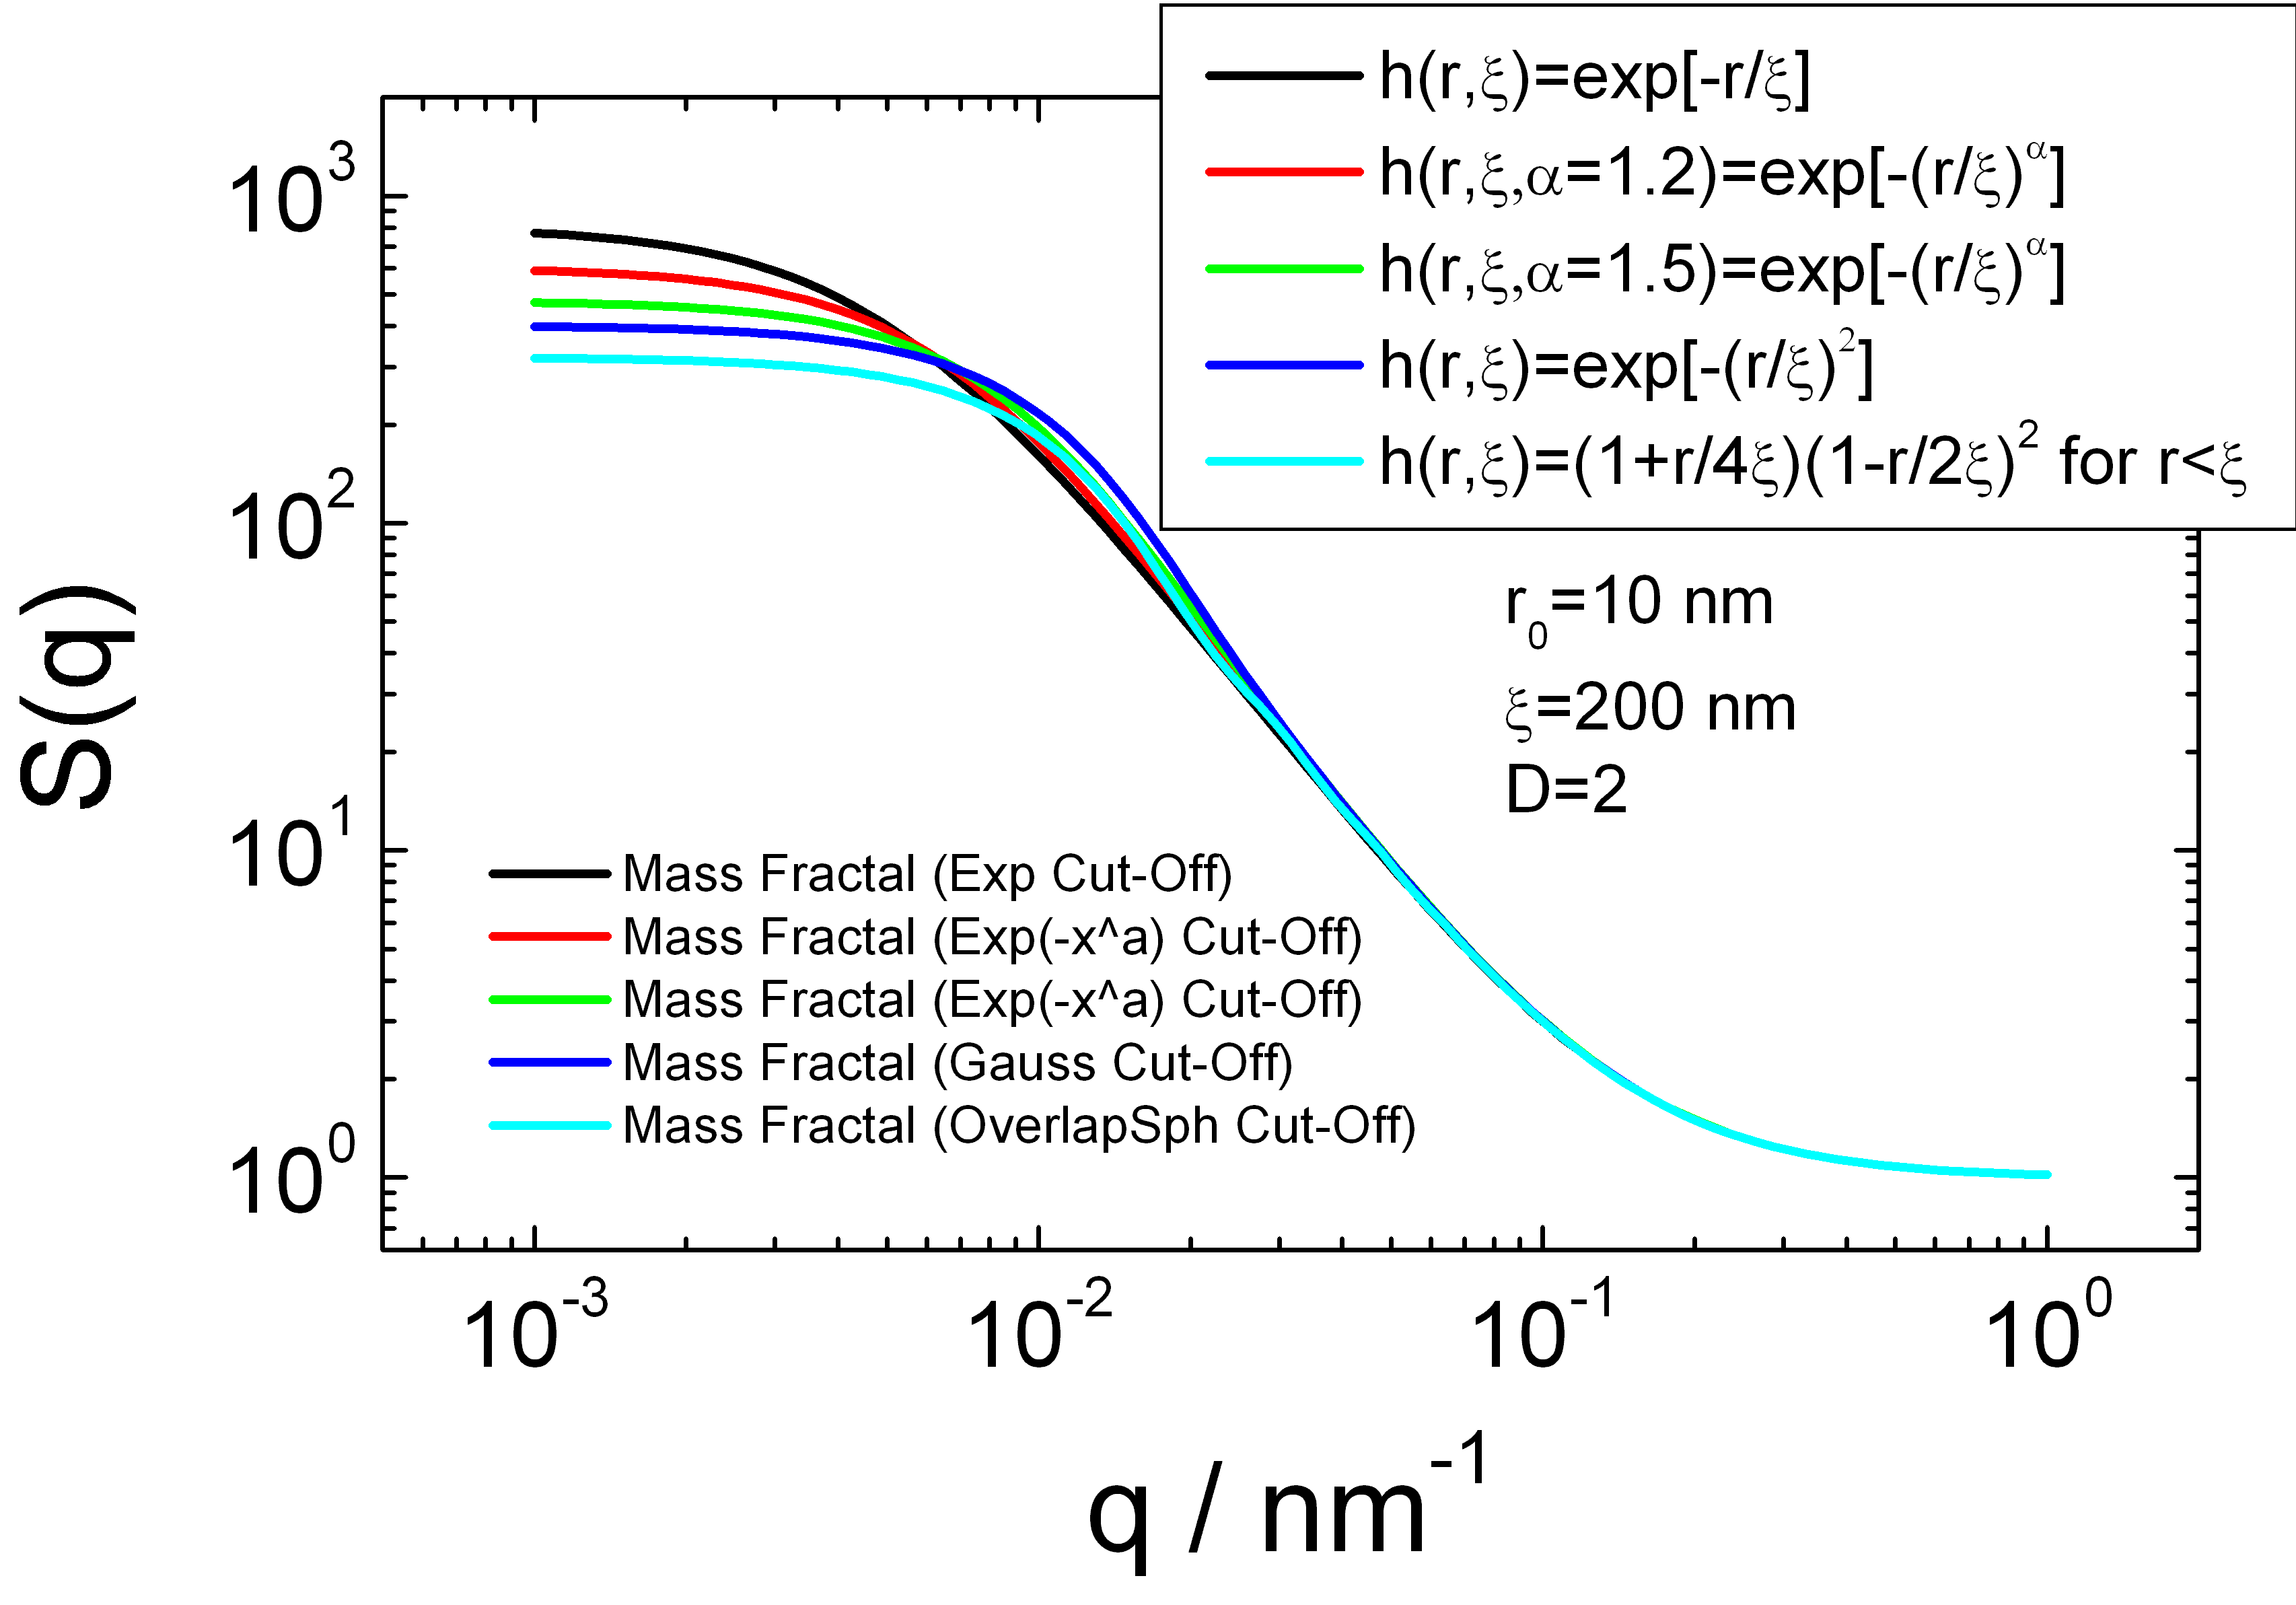
\includegraphics[width=0.768\textwidth]{../images/structure_factor/MassFractals/ComparingSQMassFractals.png}
\end{center}
\caption{Comparison of the different structure factors for mass
fractals.} \label{fig:MassFractCompare}
\end{figure}


\clearpage
\subsection{Mass Fractal (Exp Cut-Off)}
~\\
The cut-off function for this type of fractal is given by eq.\ \ref{eq:hExp} as
$h_\text{Exp}(r,\xi) = \exp\left[-\tfrac{r}{\xi}\right]$. Its structure factor is given analytically by
\begin{align}
S_\text{Exp}(q,\xi,D,r_0) &= 1 +  \cfrac{D \Gamma(D-1)
\sin\left([D-1]\arctan(q \xi)\right)}{\left( q r_0\right)^D
\left[1+\tfrac{1}{q^2\xi^2}\right]^{(D-1)/2}}
\end{align}
In the limit of $q \to 0$ the structure factor should be equal to the number $N$ of particles in the aggregate, For this type of mass fractal structure factor this limit is given by
\begin{align}\label{eq:fractalExp}
  N-1 & =\lim_{q\to 0}  S_\text{Exp}(q,\xi,D,r_0)-1 = D\Gamma(D) \frac{\xi^D}{r_0^D}
\end{align}
This allows to rewrite the structure factor also as a function of $N$ instead of $r_0$
\begin{align}
S_\text{Exp}(q,\xi,D,N) &= 1 +  (N-1)\cfrac{
\sin\left([D-1]\arctan(q \xi)\right)}{(D-1)\left( q \xi\right)^D
\left[1+\tfrac{1}{q^2\xi^2}\right]^{(D-1)/2}}
\end{align}

\uline{Input Parameters for model \texttt{Mass Fractal (Exp Cut-Off)}:}
\begin{description}
\item[\texttt{r0}] characteristic dimension of individual scattering objects $r_0$
\item[\texttt{xi}] cut-off length for the fractal correlations $\xi$
\item[\texttt{D}] fractal dimension $D$
\end{description}

\uline{Note:}
\begin{itemize}
\item $D$ needs to be larger than 1 ($D>1$). Physical values for $D$ are between 1 and 3 ($1<D<3$).
\item The fractal dimension needs to be larger than the size of the individual scattering objects ($r_0 < \xi$).
\item The number of particles in the aggregate should be larger or equal to 1 $(N\geq 1)$
\end{itemize}

\begin{figure}[htb]
\begin{center}
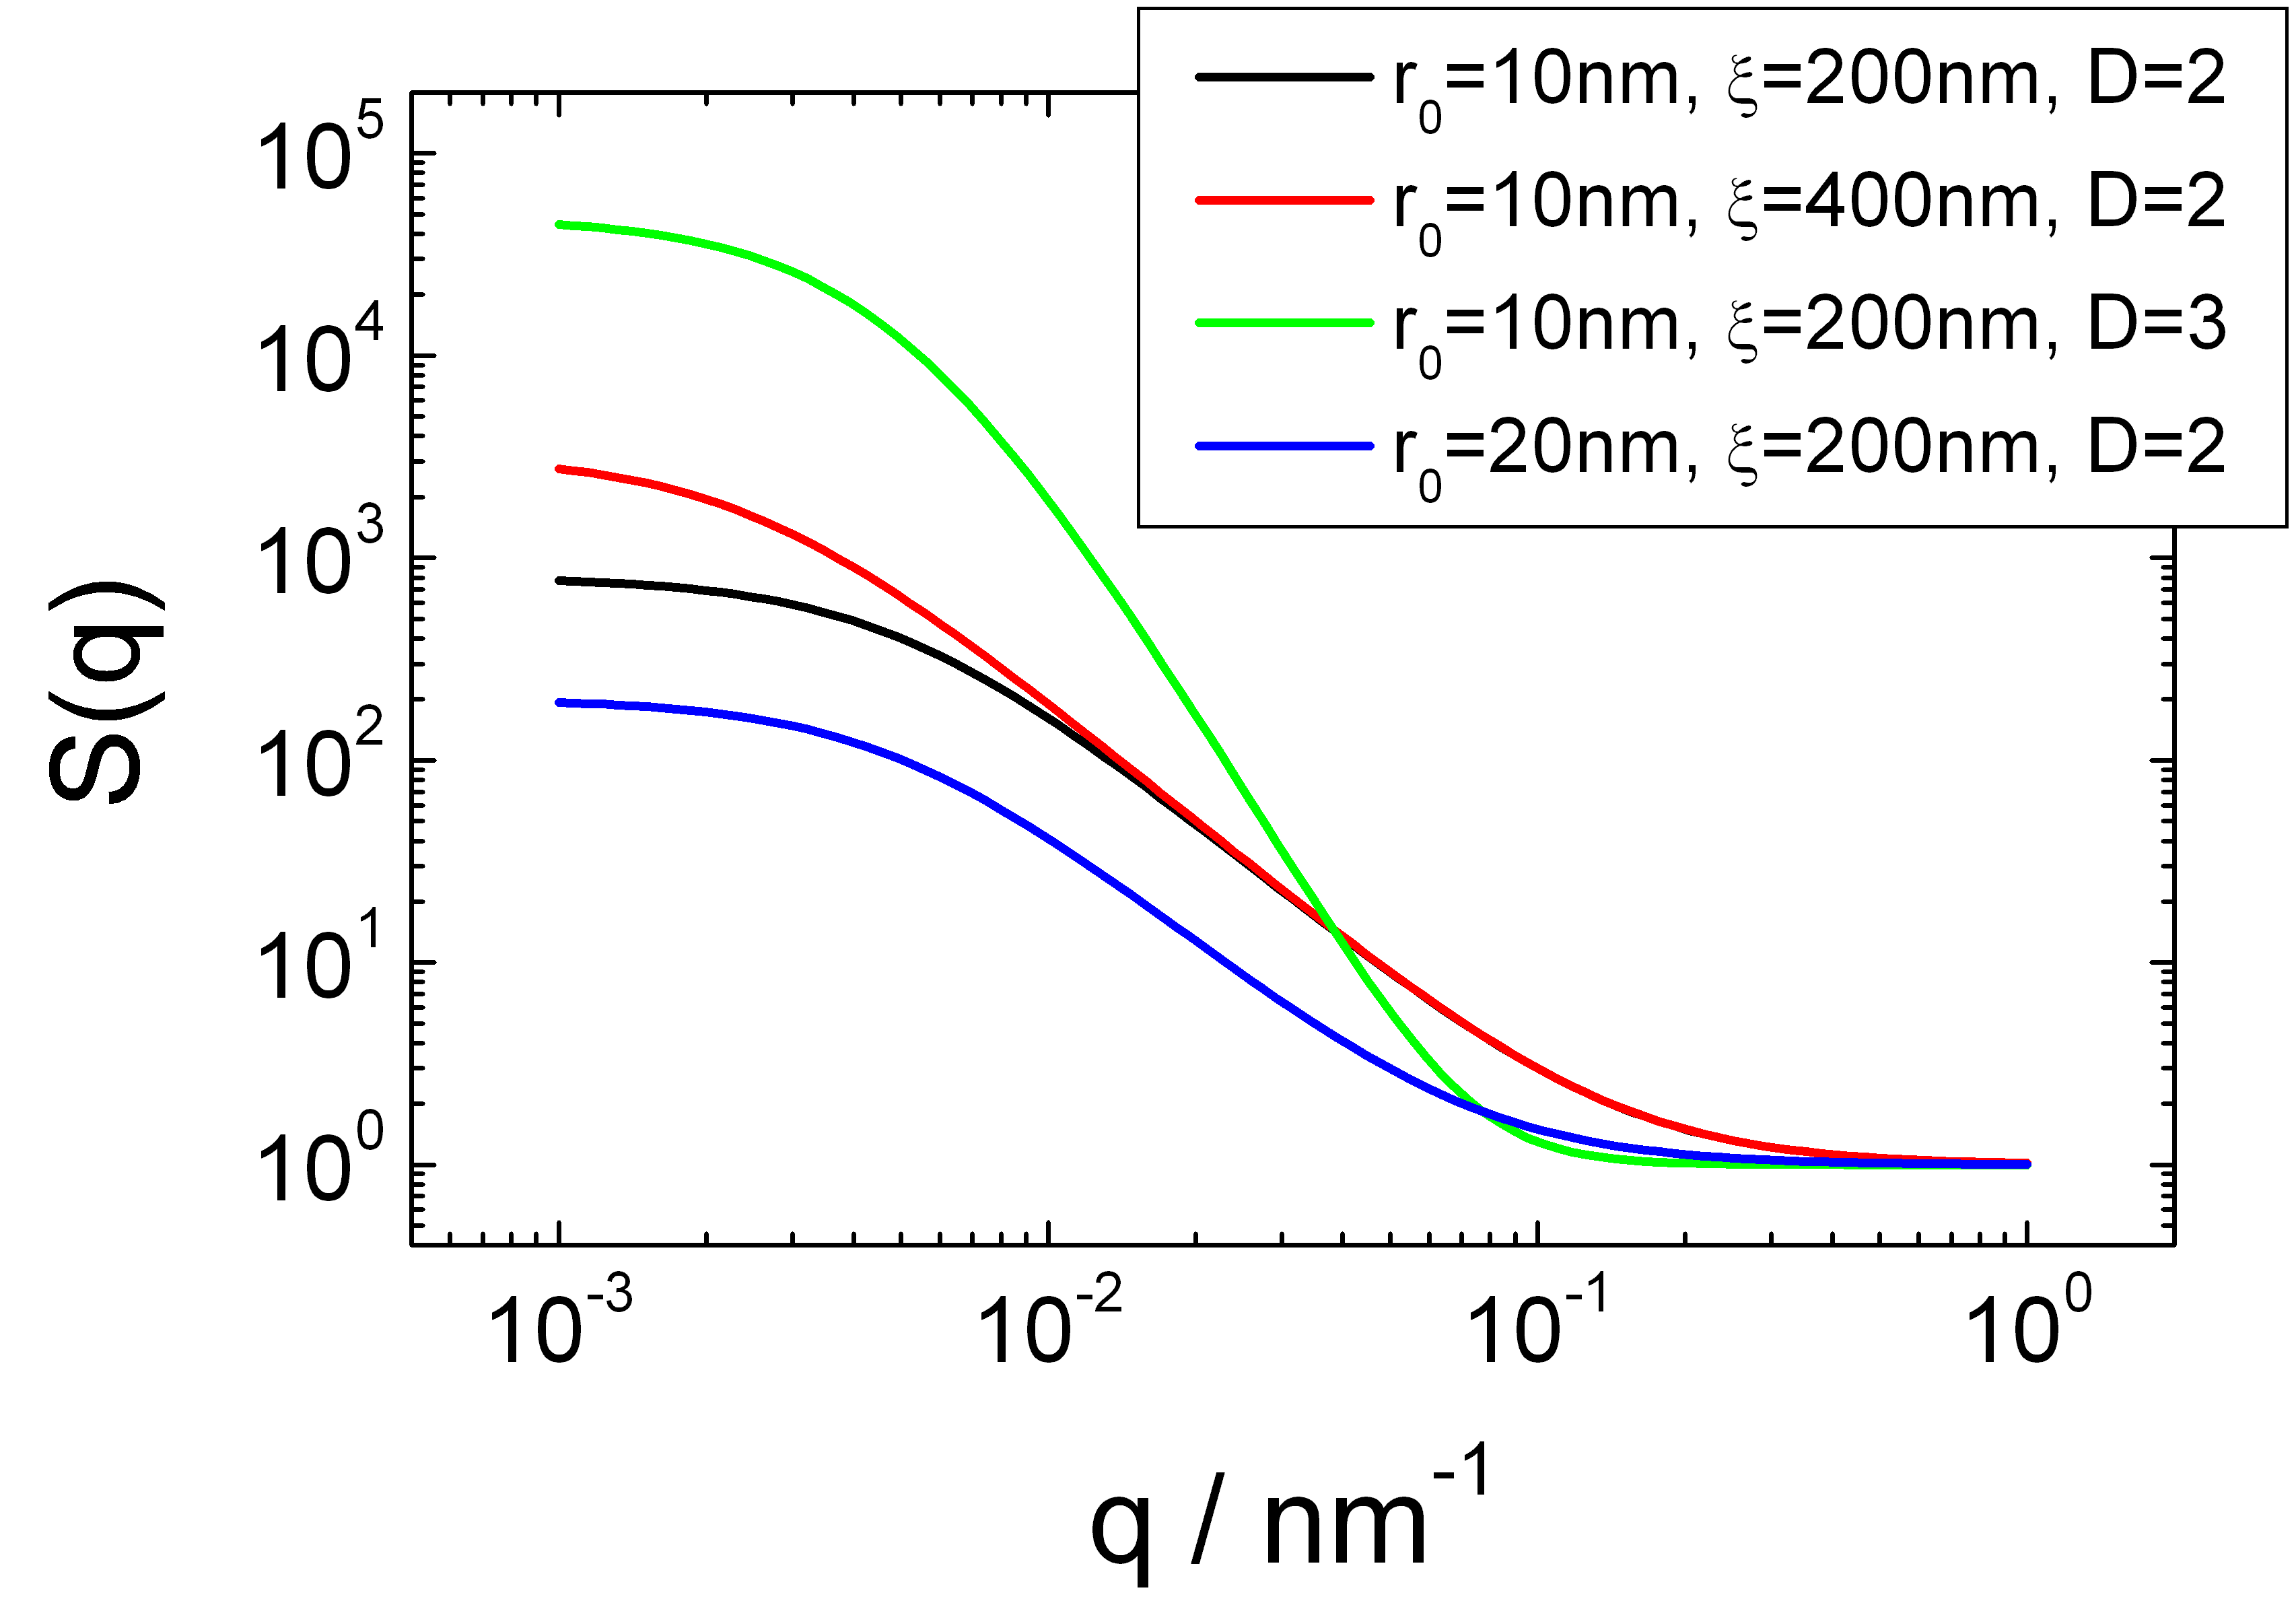
\includegraphics[width=0.6\textwidth]{../images/structure_factor/MassFractals/SQExpCutOff.png}
\end{center}
\caption{Structure factor of a mass fractal with an exponential
cut-off function $h_\text{Exp}(r,\xi) = \exp\left[-\tfrac{r}{\xi}\right]$.}
\label{fig:SQExpCutOff}
\end{figure}


\clearpage
\subsection{Mass Fractal (Exp(-x\^{}a) Cut-Off)}
~\\

\uline{Input Parameters for model \texttt{Mass Fractal (Exp(-x\^{}a) Cut-Off)}:}
\begin{description}
\item[\texttt{r0}] characteristic dimension of individual scattering objects $r_0$
\item[\texttt{xi}] cut-off length for the fractal correlations $\xi$
\item[\texttt{D}] fractal dimension $D$
\end{description}

\uline{Note:}
\begin{itemize}
\item $D$ needs to be larger than 1 ($D>1$). Physical values for $D$ are between 1 and 3 ($1<D<3$).
\item The fractal dimension needs to be large than the size of the individual scattering objects ($r_0 < \xi$).
\item the exponents $\alpha$ should be larger than 1, as otherwise the integral \ref{eq:hSQ} for $S(q)$ does not converges.
\end{itemize}

\begin{figure}[htb]
\begin{center}
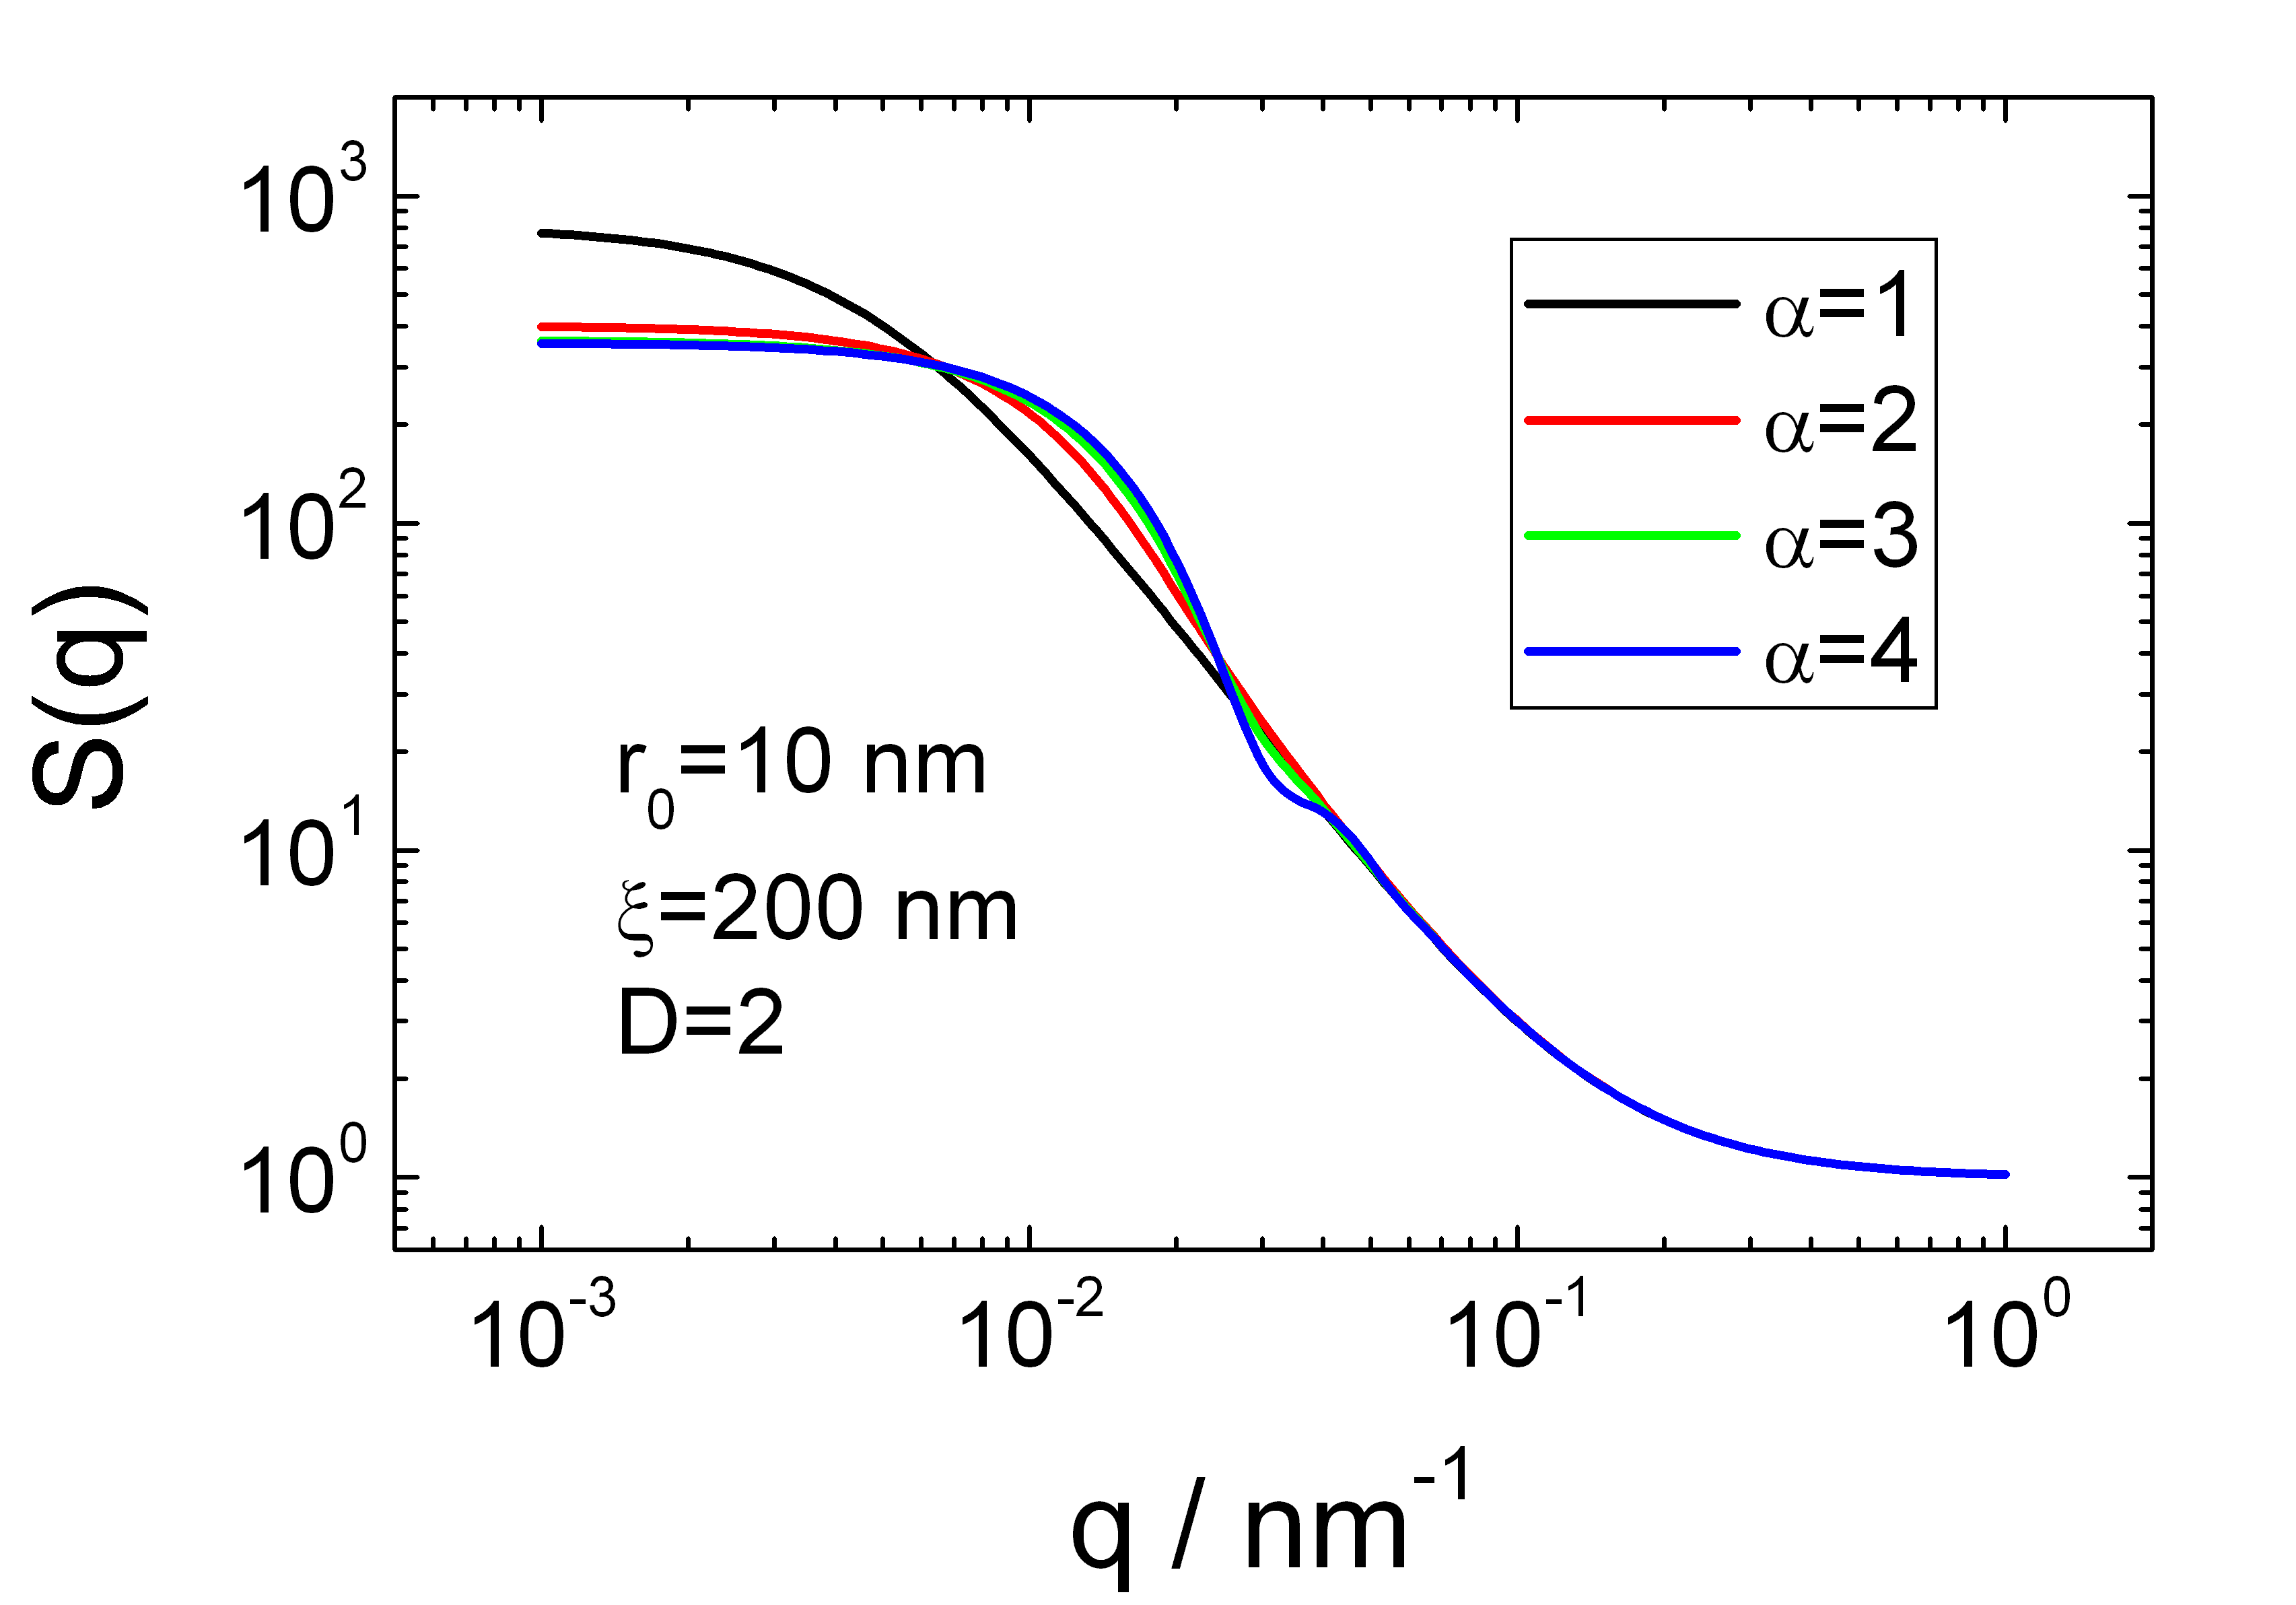
\includegraphics[width=0.768\textwidth]{../images/structure_factor/MassFractals/SQExp(pow(x,a))CutOff.png}
\end{center}
\caption{Structure factor of a mass fractal with a cut-off function
$h_\text{Exp(-x$\hat{~}$a)}(r,\xi,\alpha) = \exp\left[-\left(\tfrac{r}{\xi}\right)^\alpha\right]$.}
\label{fig:SQExpxaCutOff}
\end{figure}


\clearpage
\subsection{Mass Fractal (Gaussian Cut-Off)}
~\\

The cut-off function for this type of fractal is given by eq.\ \ref{eq:hGauss} as
$h_\text{Exp}(r,\xi) = \exp\left[-\left(\tfrac{r}{\xi}\right)^2\right]$. Its structure factor is given analytically by
\begin{align}
S_\text{Gauss}(q,\xi,D,r_0) &= 1 +
    \Gamma\left[\tfrac{D}{2}\right]\frac{D}{2}
    \left(\frac{\xi}{r_0}\right)^D
    {}_1F_1\left[\tfrac{D}{2},\tfrac{3}{2},-\tfrac{q^2\xi^2}{8}\right]
\end{align}
In the limit of $q \to 0$ the structure factor should be equal to the number $N$ of particles in the aggregate, For the mass fractal structure factor this limit is given by
\begin{align}\label{eq:fractalGauss}
  N-1 & =\lim_{q\to 0}  S_\text{Gauss}(q,\xi,D,r_0)-1 = \frac{D}{2}\Gamma\left( \frac{D}{2} \right) \frac{\xi^D}{r_0^D}
\end{align}
This allows to rewrite the structure factor also as a function of $N$ instead of $r_0$
\begin{align}
S_\text{Gauss}(q,\xi,D,N) &= 1 +  (N-1) {}_1F_1\left[\tfrac{D}{2},\tfrac{3}{2},-\tfrac{q^2\xi^2}{8}\right]
\end{align}


\uline{Input Parameters for model \texttt{Mass Fractal (Gaussian Cut-Off)}:}
\begin{description}
\item[\texttt{r0}] characteristic dimension of individual scattering objects $r_0$
\item[\texttt{xi}] cut-off length for the fractal correlations $\xi$
\item[\texttt{D}] fractal dimension $D$
\end{description}

\uline{Note:}
\begin{itemize}
\item $D$ needs to be larger than 1 ($D>1$). Physical values for $D$ are between 1 and 3 ($1<D<3$).
\item The fractal dimension needs to be large than the size of the individual scattering objects ($r_0 < \xi$).
\item The number of particles in the aggregate should be larger or equal to 1 $(N\geq 1)$
\end{itemize}

\begin{figure}[htb]
\begin{center}
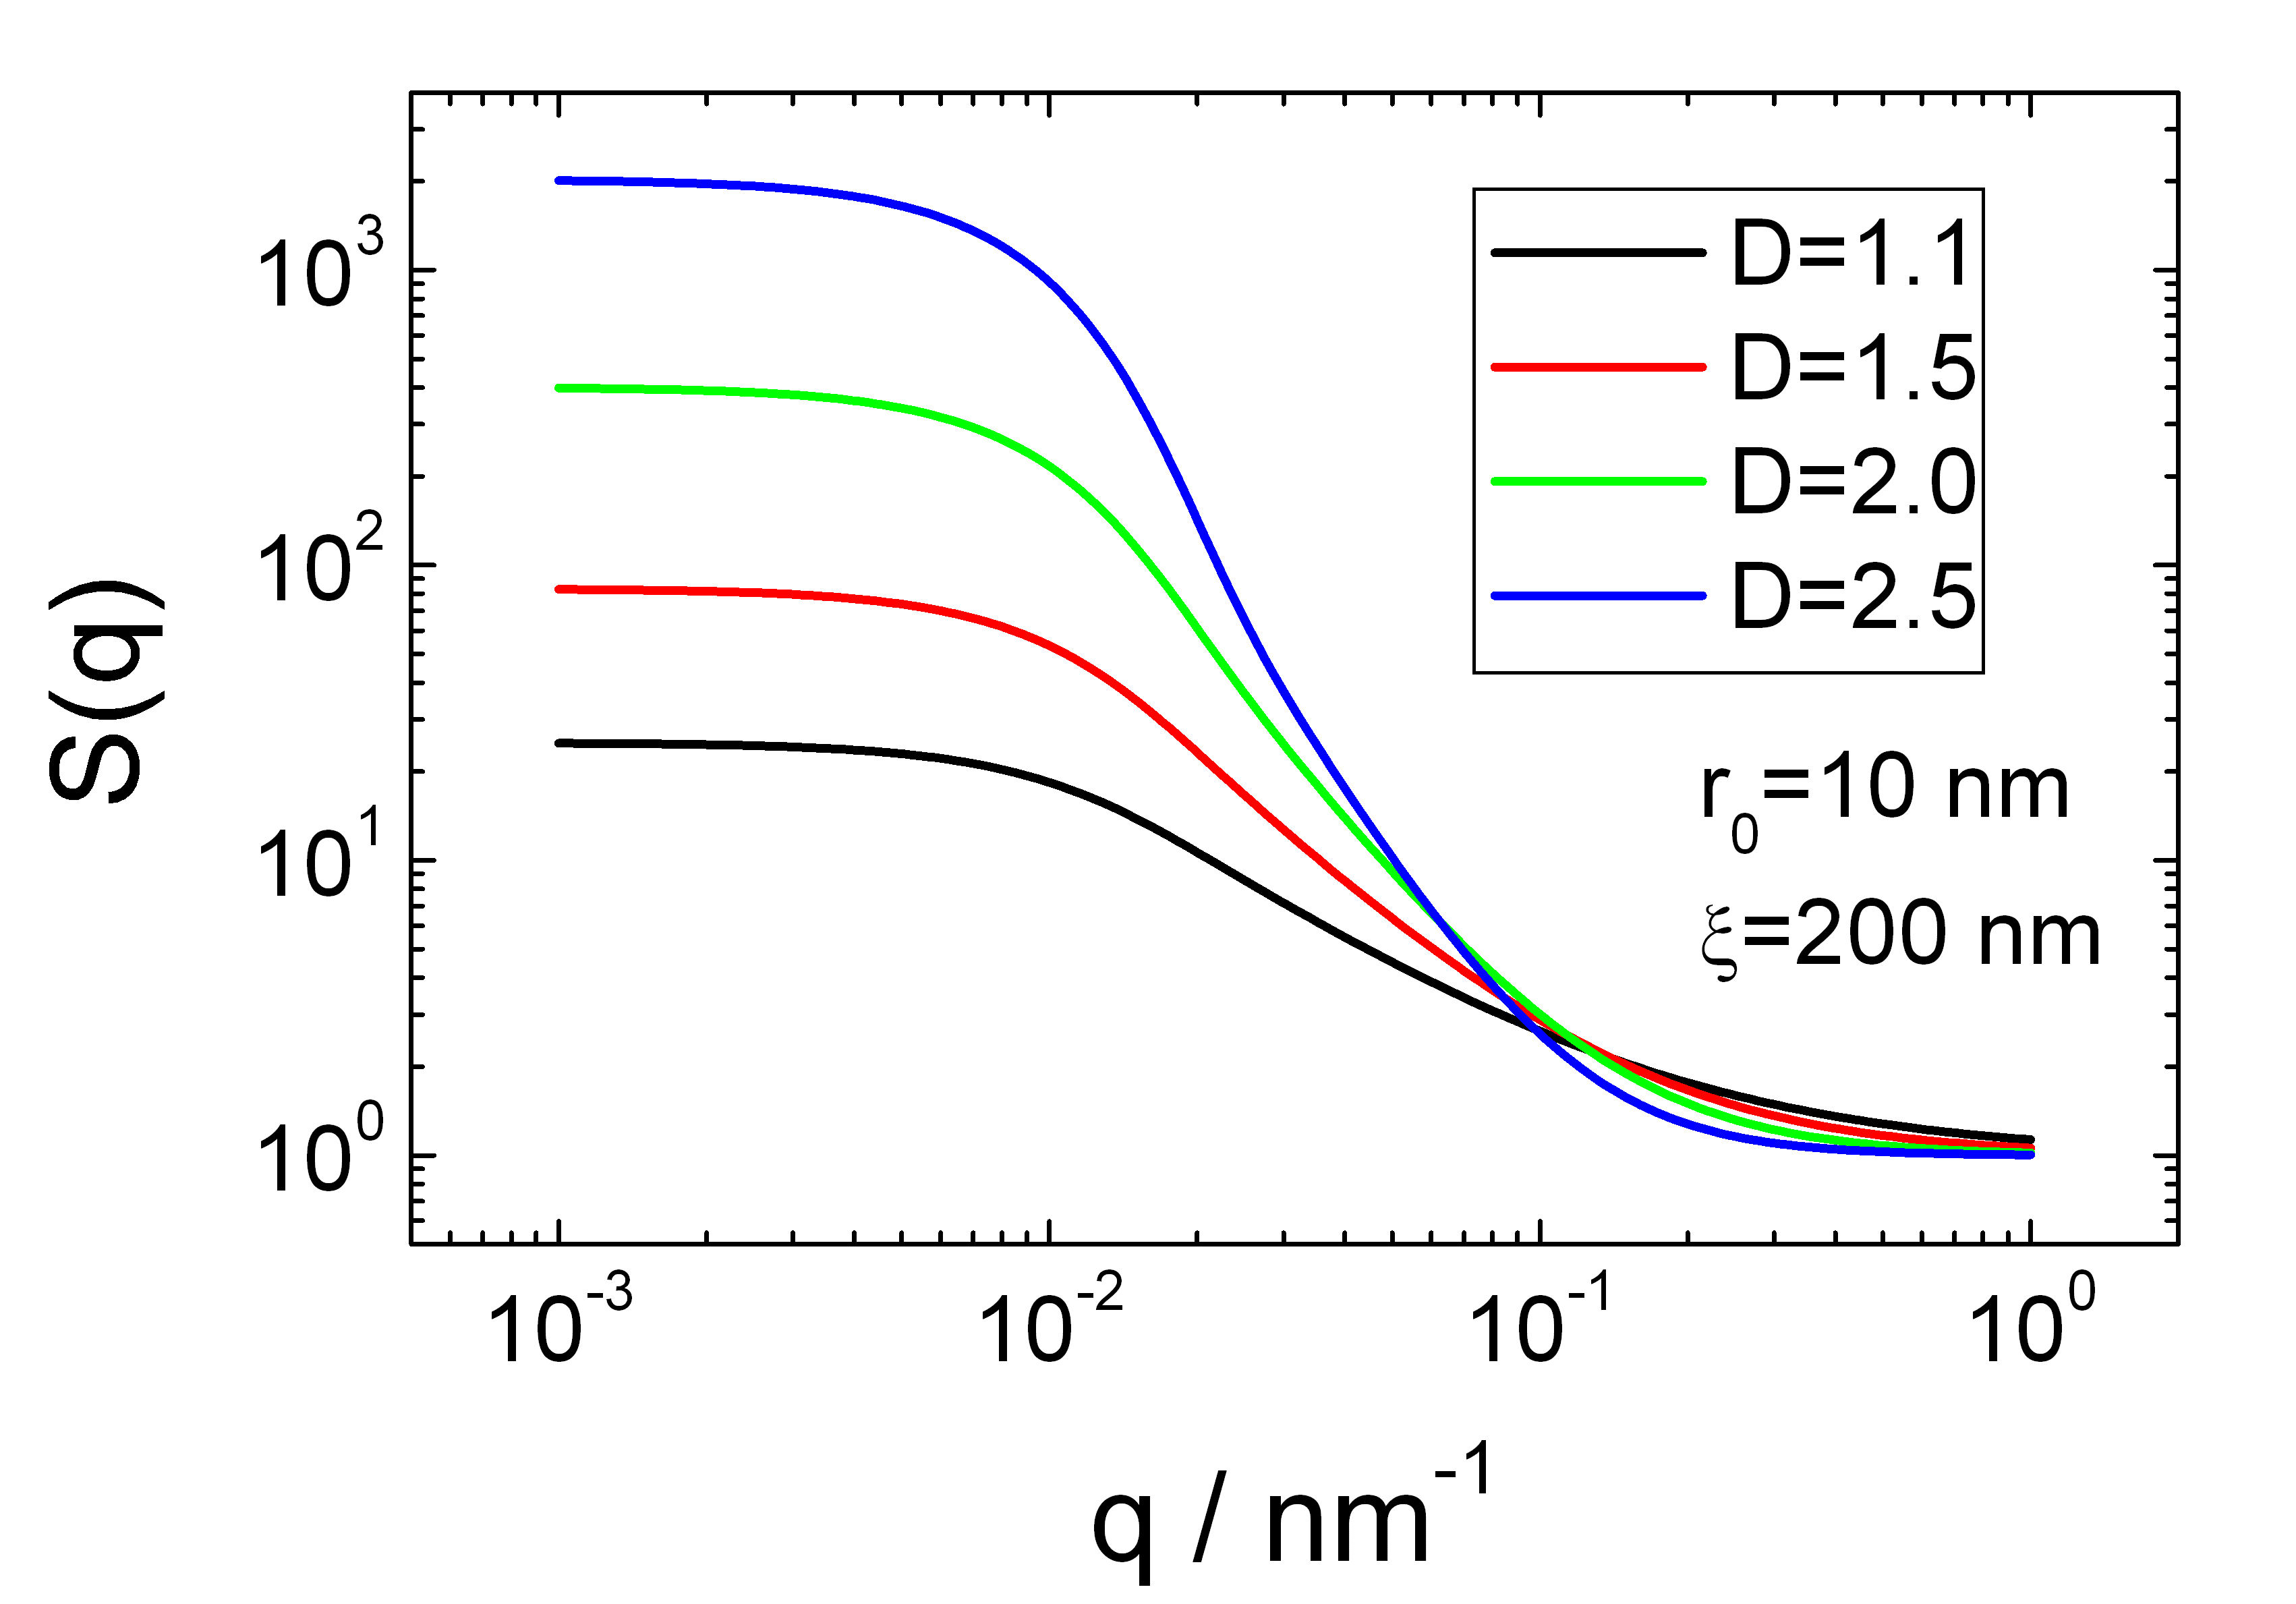
\includegraphics[width=0.6\textwidth]{../images/structure_factor/MassFractals/SQGaussCutOff.png}
\end{center}
\caption{Structure factor of a mass fractal with an Gaussian
cut-off function $h_\text{Gauss}(r,\xi) = \exp\left[-\left(\tfrac{r}{\xi}\right)^2\right]$.}
\label{fig:SQGaussCutOff}
\end{figure}


\clearpage
\subsection{Mass Fractal (OverlapSph Cut-Off)}
~\\
In the limit of $q \to 0$ the structure factor should be equal to the number $N$ of particles in the aggregate, For the mass fractal structure factor this limit is given by
\begin{align}\label{eq:fractalGauss}
  N-1 & =\lim_{q\to 0}  S_\text{OverlapSph}(q,\xi,D,r_0)-1 = \frac{3D 2^D}{D^3+4D^2+3D} \,\, e\frac{\xi^D}{r_0^D}
\end{align}
\uline{Input Parameters for model \texttt{Mass Fractal (OverlapSph Cut-Off)}:}
\begin{description}
\item[\texttt{r0}] characteristic dimension of individual scattering objects $r_0$
\item[\texttt{xi}] cut-off length for the fractal correlations $\xi$
\item[\texttt{D}] fractal dimension $D$
\end{description}

\uline{Note:}
\begin{itemize}
\item $D$ needs to be between 1 and 3 ($1<D<3$).
\item The fractal dimension needs to be large than the size of the individual scattering objects ($r_0 < \xi$).
\end{itemize}

\begin{figure}[htb]
\begin{center}
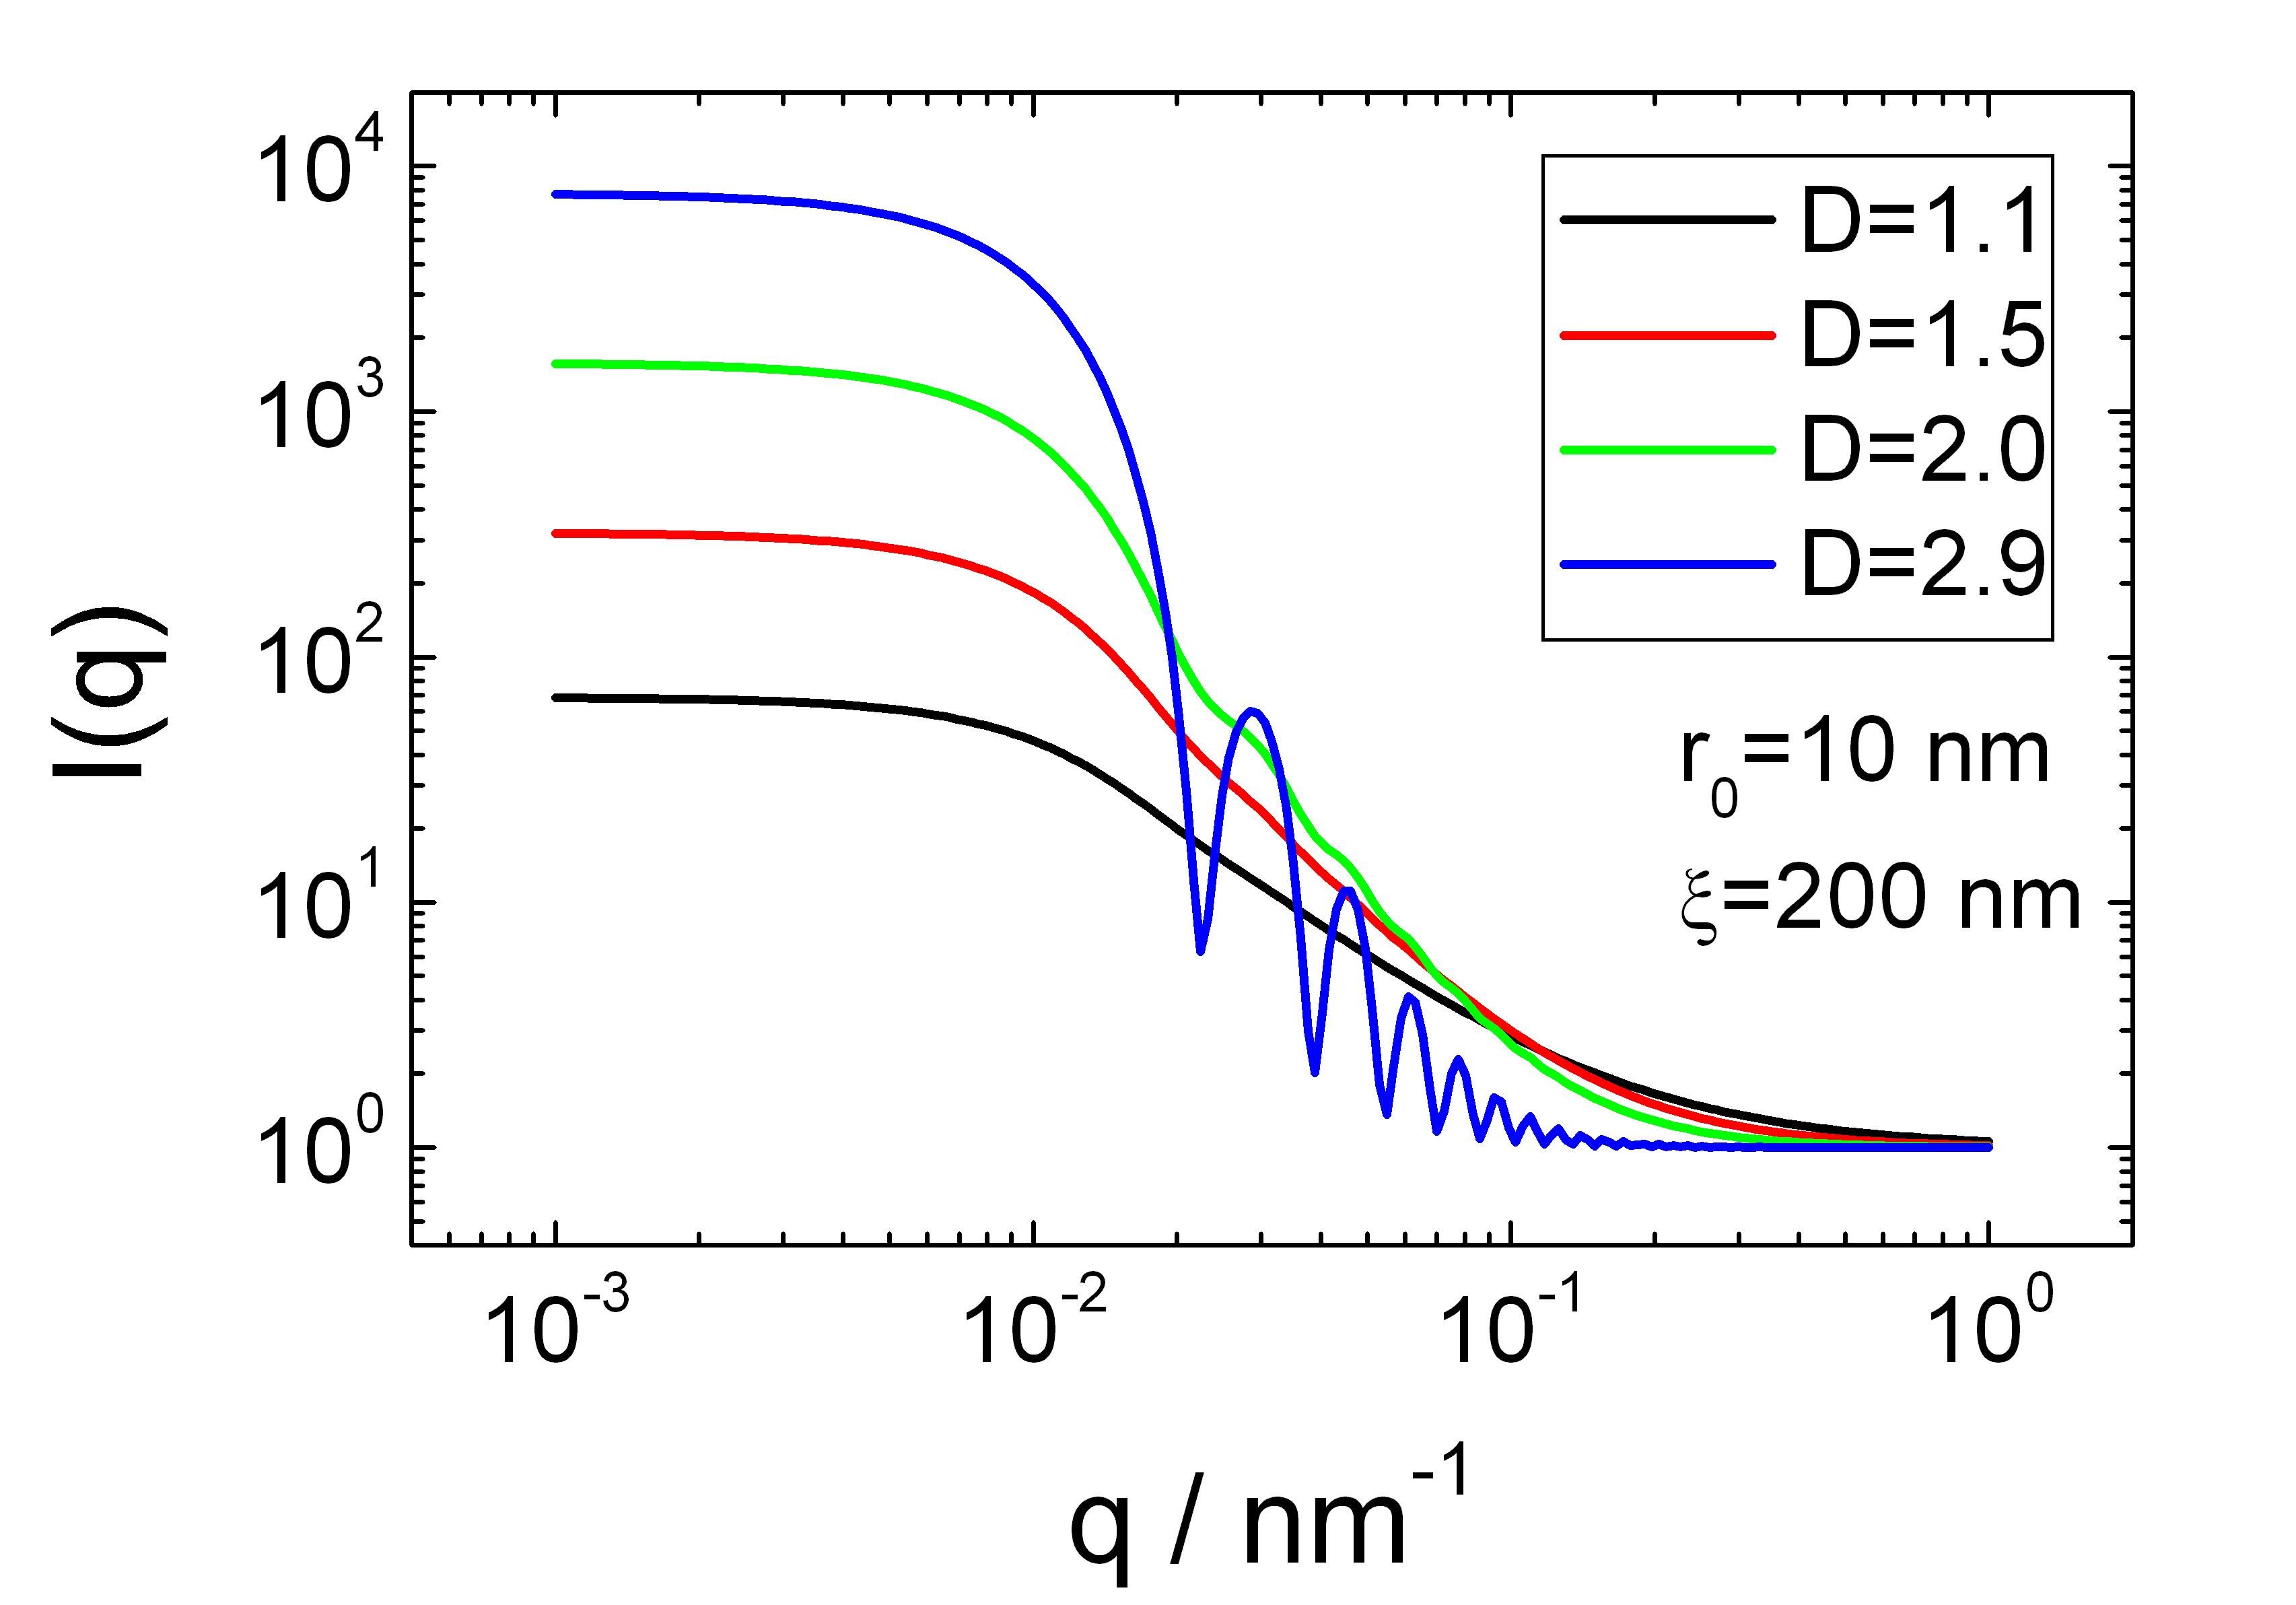
\includegraphics[width=0.768\textwidth]{../images/structure_factor/MassFractals/SQOverlapSphCutOff.png}
\end{center}
\caption{Structure factor of a mass fractal with a
cut-off function $h_\text{OverlapSph}(r,\xi) = \left(1+\frac{r}{4\xi}\right)\left(1-\frac{r}{2\xi}\right)^2$ for $r\leq 2\xi$.}
\label{fig:SQOverlappSphCutOff}
\end{figure}

\clearpage
%%%%%%%%%%%%%%%%%%%%%%%%%%%%%%%%%%%%%%%%%%%%%%%%%%%%%%%%%%%%%%%%%%%%%%%%%%%%%%%%%%%%%%%%
\subsection{Structure factor of a random flight model} \hspace{1pt}\\
The random flight model describes a discrete chain, where the positions of the $N$ units forming the discrete chains follow a 3D random walk. The distance between neighbouring units is constants.

\begin{figure}[htb]
\begin{center}
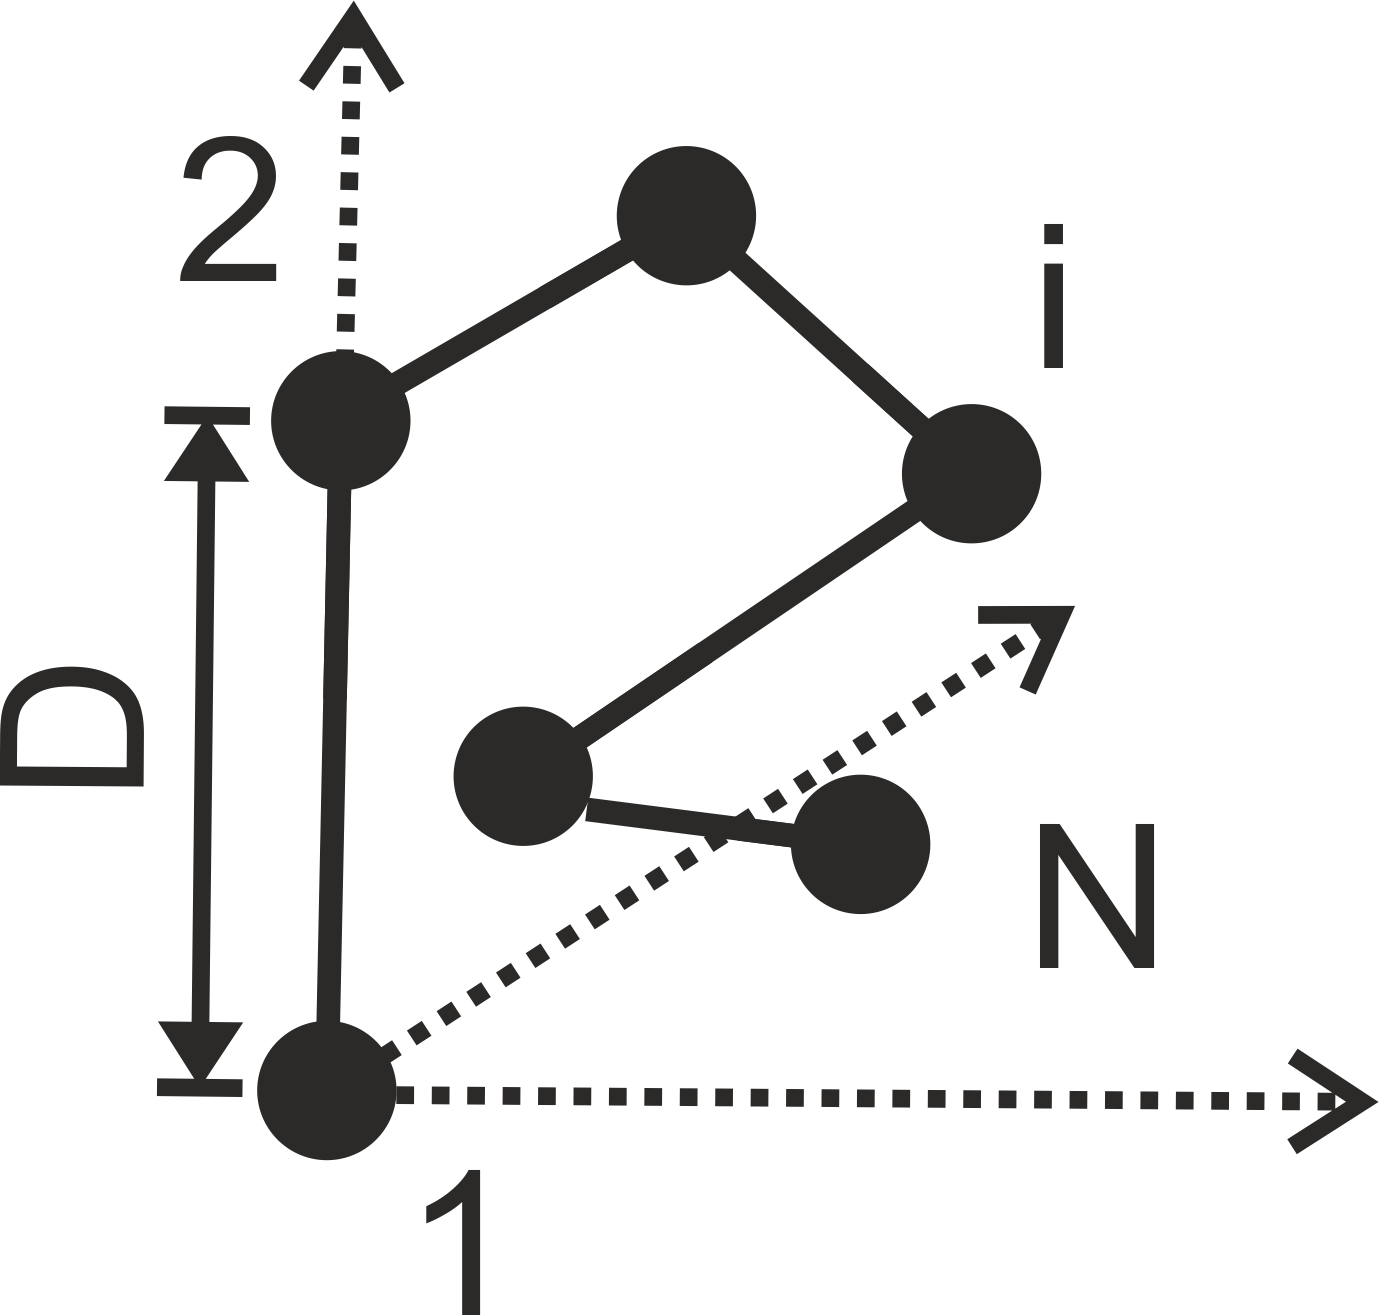
\includegraphics[width=0.35\textwidth]{../images/structure_factor/randomflight3D.png}
\end{center}
\caption{Random flight of $N$ particles with constant distances $D$.}
\label{fig:randomflight3D}
\end{figure}

\begin{figure}[htb]
\begin{center}
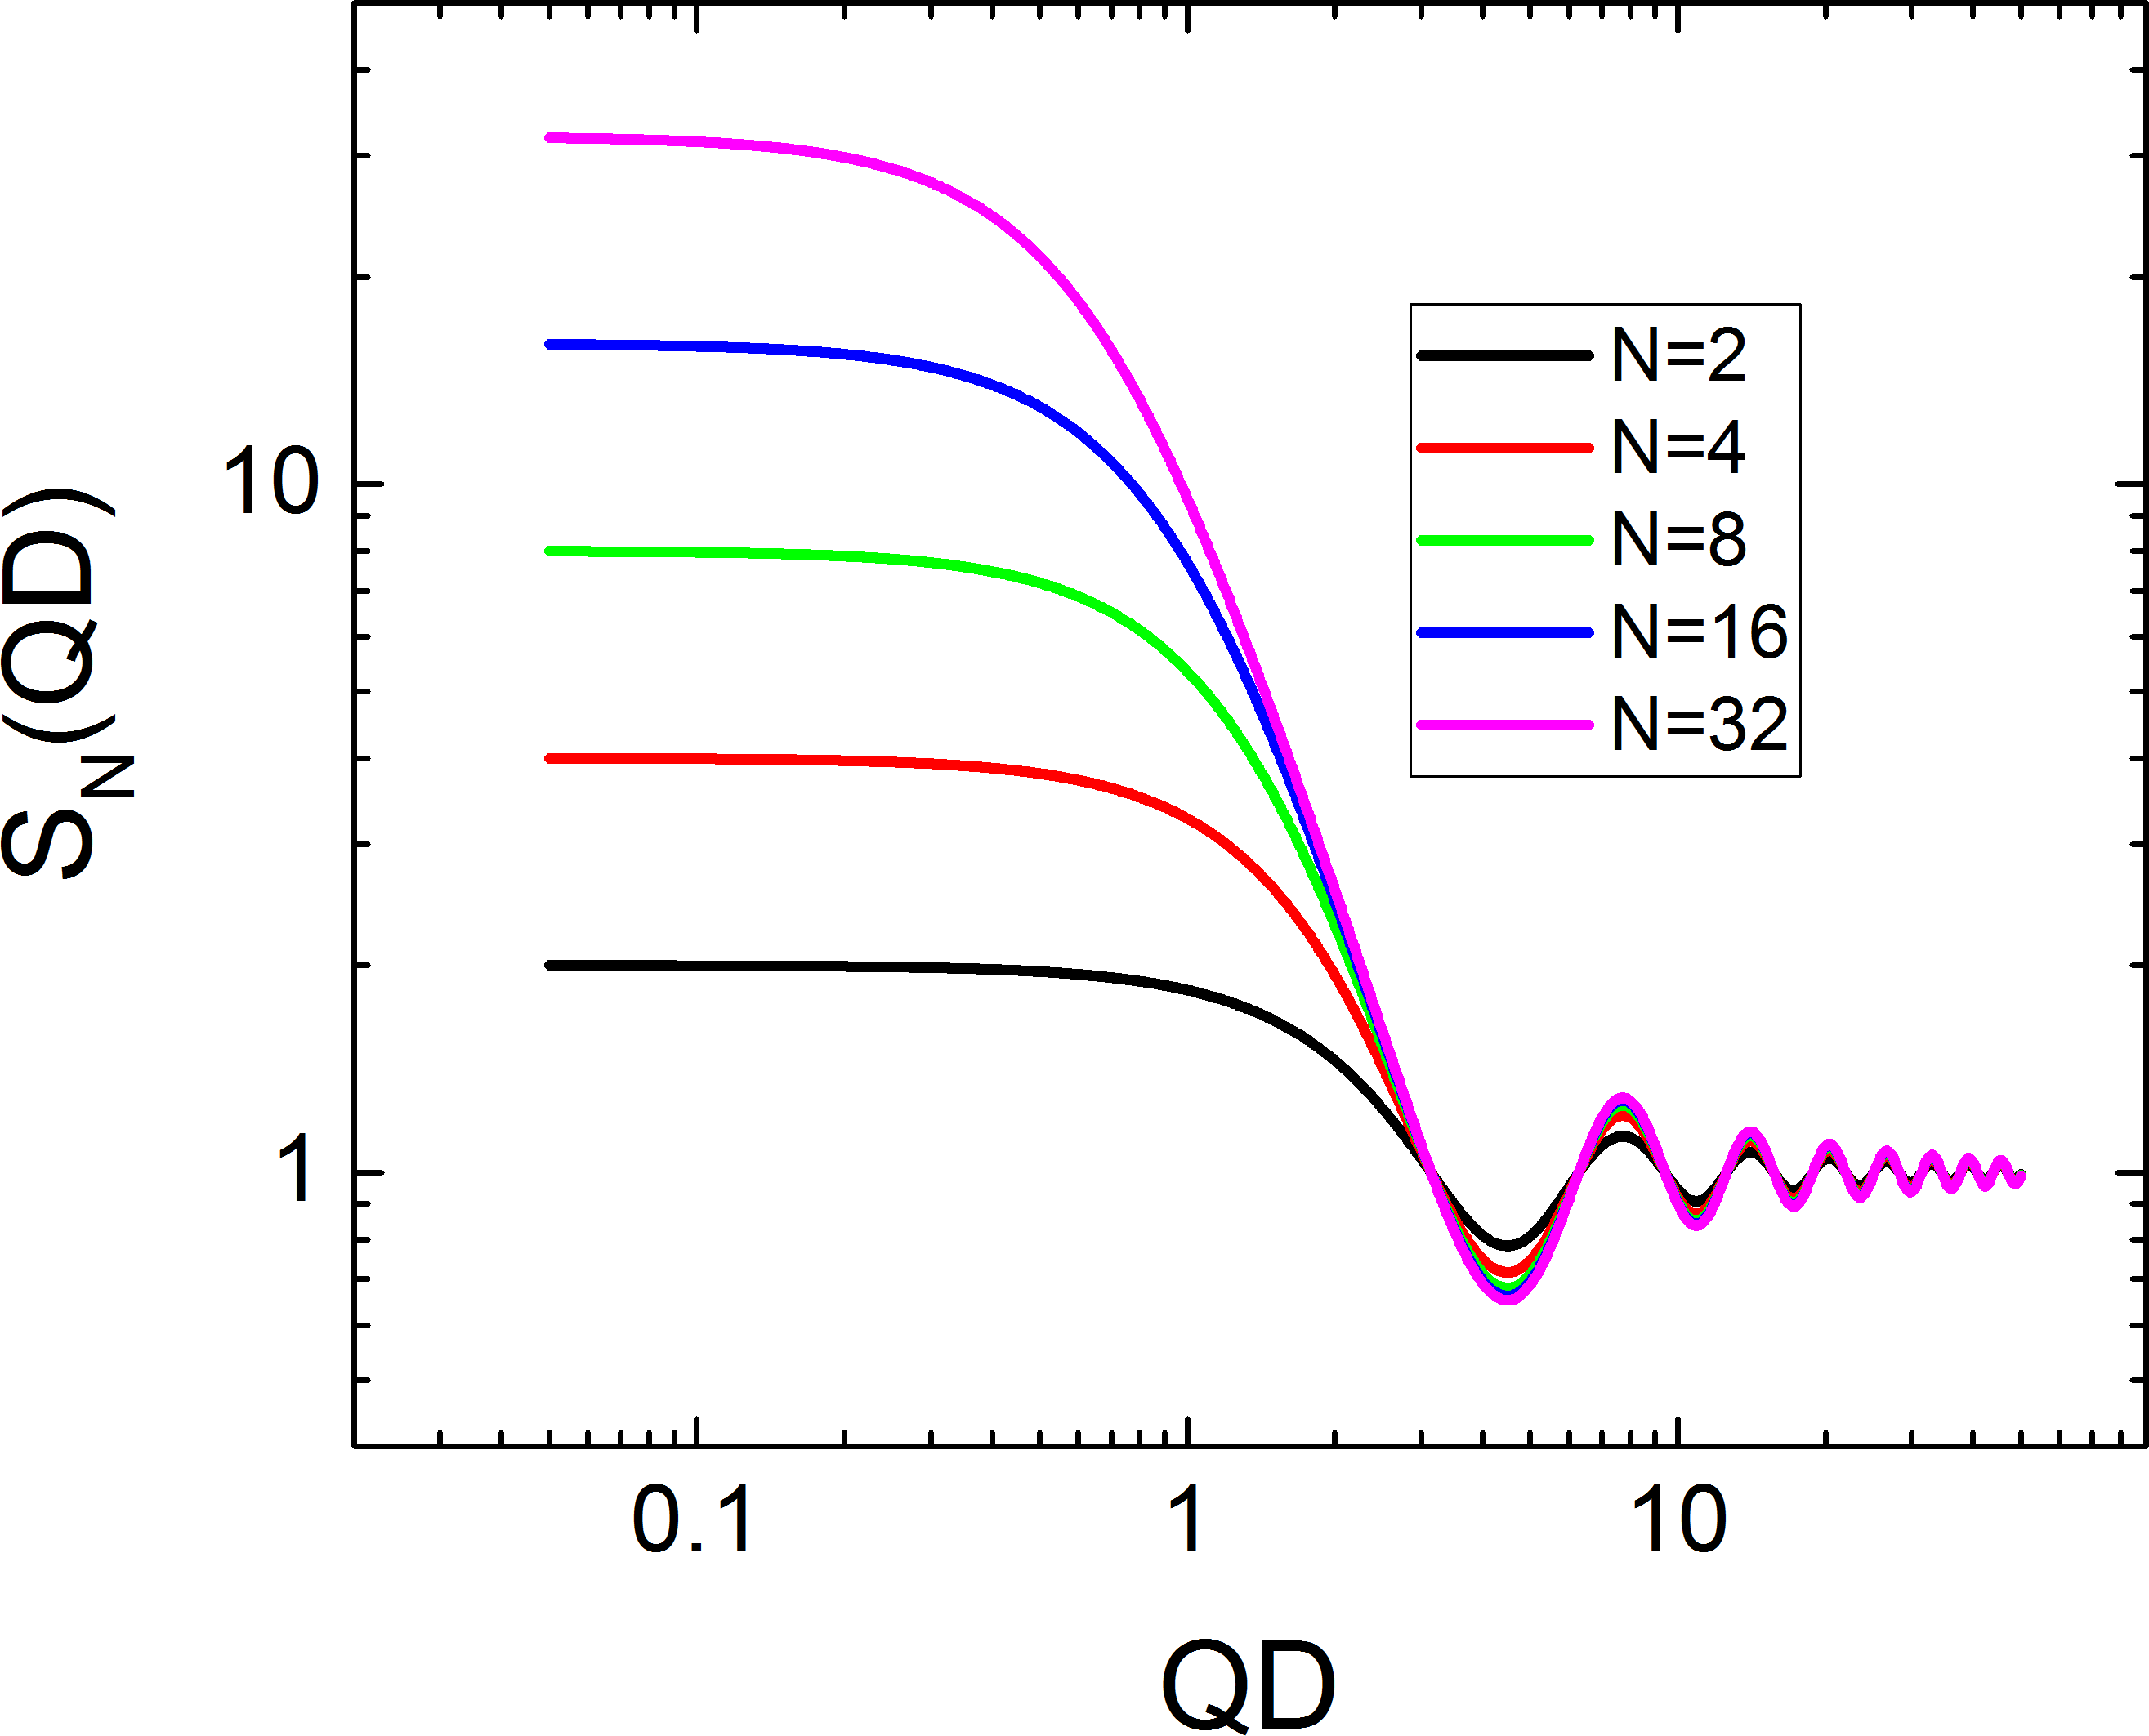
\includegraphics[width=0.5\textwidth]{../images/structure_factor/randomflight.png}
\end{center}
\caption{Random flight structure factor with $N$ steps of length $D$.}
\label{fig:randomflight}
\end{figure}

The structure factor $S_N(QD)$ describing such an arrangement of $N$ particles on a random flight
with a constant step size $D$ is given by \cite{Burchard1970} as
\begin{align}
S_N(QD)=& 1+2\sum_{k=1}^{k=N-1}\left(1-\frac{k}{N}\right)\left[\frac{\sin(QD)}{QD}\right]^k \\
    &\frac{2}{1-\frac{\sin(QD)}{QD}}-1-\frac{2\left[1-\left[\frac{\sin(QD)}{QD}\right]^N\right]}{N\left[1-\frac{\sin(QD)}{QD}\right]^2}\frac{\sin(QD)}{QD}
\end{align}
The formula above is only real for all values of $QD$ for integer values of $N$. For non integer values $N$ a linear interpolation between $[N]$ and $[N]+1$ is taken \cite{Giehm2010}, where $[N]$ is the largest integer smaller or equal to $N$. With $w=N-[N]$ we get
\begin{align}
S_N(QD)&= (1-w)S_{[N]}(QD) + wS_{[N]+1}(QD)
\end{align}

\noindent \uline{Input Parameters for model \texttt{random flight}:}\\
\begin{description}
\item[\texttt{D}] step length $D$
\item[\texttt{n}] number of steps $N$
\end{description}


\noindent\uline{Note:}
\begin{itemize}
\item $N$ needs to be larger or equal to 1. For non-integer values of $N$ the curve is linear interpolated between the structure factor for $N$ and $N+1$.
\end{itemize}

\subsection{ Structure factor of a random flight model with a paracrystalline like disorder parameter}~\\ \label{sec:pcRandomFlight}
\begin{align}\label{eq:pcRFsum}
  S_N(Q,D,\Delta) =&  1+2 \sum _{k=1}^{N-1} \left(1-\frac{k}{N}\right) \left(\frac{\sin (D Q)}{D
   Q}\right)^k \exp \left(-\frac{1}{2} k \Delta^2 Q^2\right) \\
   \begin{split} =& \quad
   \frac{Q^2 D^2 e^{\Delta^2 Q^2}-\sin^2 (Q D) }{
   \left(\sin (QD)-QD e^{\frac{\Delta^2 Q^2}{2}}\right)^2} \quad +\\
        &  \quad
   \frac{\sin (Q D) \left(2 Q D
   \left(e^{-\frac{(N-1)\Delta^2  Q^2}{2}} \left(\frac{\sin (QD)}{Q
   D}\right)^N-e^{\frac{\Delta^2 Q^2}{2}}\right)\right)}{N
   \left(\sin (QD)-QD e^{\frac{\Delta^2 Q^2}{2}}\right)^2}
   \end{split} \label{eq:pcRFanalytical}
\end{align}

\noindent \uline{Input Parameters for model \texttt{PC:random flight}:}\\
\begin{description}
\item[\texttt{D}] step length $D$
\item[\texttt{n}] number of steps $N$
\item[\texttt{n}] paracrystalline-like disorder parameter $\Delta$
\end{description}

\noindent\uline{Note:}
\begin{itemize}
\item $N$ needs to be larger or equal to 1. For non-integer values of $N$ the curve is linear interpolated between the structure factor for $N$ and $N+1$.
\end{itemize}

\subsection{Extended cluster structure factor with local hardsphere
interactions}~\\
\label{sec:SQec}
This structure factor assume clusters of particles with a cluster size $\xi$, whereas the particle within a cluster interact via a hard sphere potential and a local volume fraction $\phi$. In the original paper \cite{Larsen2020} the clusters are described by a spherical form factor and a Gaussian size distribution. It was also mentioned, that the polydisperse spherical form factor can be replaced by any other form factor better describing the shape of the clusters. In this implementation of the extended cluster model we use the extended Debye-Anderson-Brumberger model from section \ref{sect:epsilonDAB} describing the scattering of the clusters.
\begin{align}\label{eq:extendedClusterSQ}
  S_\mathrm{ec}(q) &= S_\mathrm{PY}(q)+\left(N-S_\mathrm{PY}(q)\right)P_{\epsilon\mathrm{DAB}}(q)\\
  P_{\epsilon\mathrm{DAB}}(q) &= I_{\epsilon\mathrm{DAB}}(q) / \left(8\pi\xi^3\epsilon\right)\\
  N &= \frac{8\pi\xi^3\epsilon}{\frac{4}{3}\pi R^3}
\end{align}
The structure factor $S_\mathrm{PY}(q)$ is described in sec.\ \ref{sec:SQ:PY} and the form factor $I_{\epsilon\mathrm{DAB}}(q)$ is defined in equations \ref{eq:DABaffPLUSrnd_eps_small} and \ref{eq:DABaffPLUSrnd_eps_large}. The volume of the DAB-particle can be obtained via the correlation function $\gamma_{0,\mathrm{DAB}}(r)=\exp(-r/\xi)$ according to eq.\ \ref{eq:VolumeFromCorrelationfunction} and is for the $\epsilon$DAB model given as $V_{\epsilon\mathrm{DAB}}=8\pi\xi^3\epsilon$.

\begin{figure}[htb]
\begin{center}
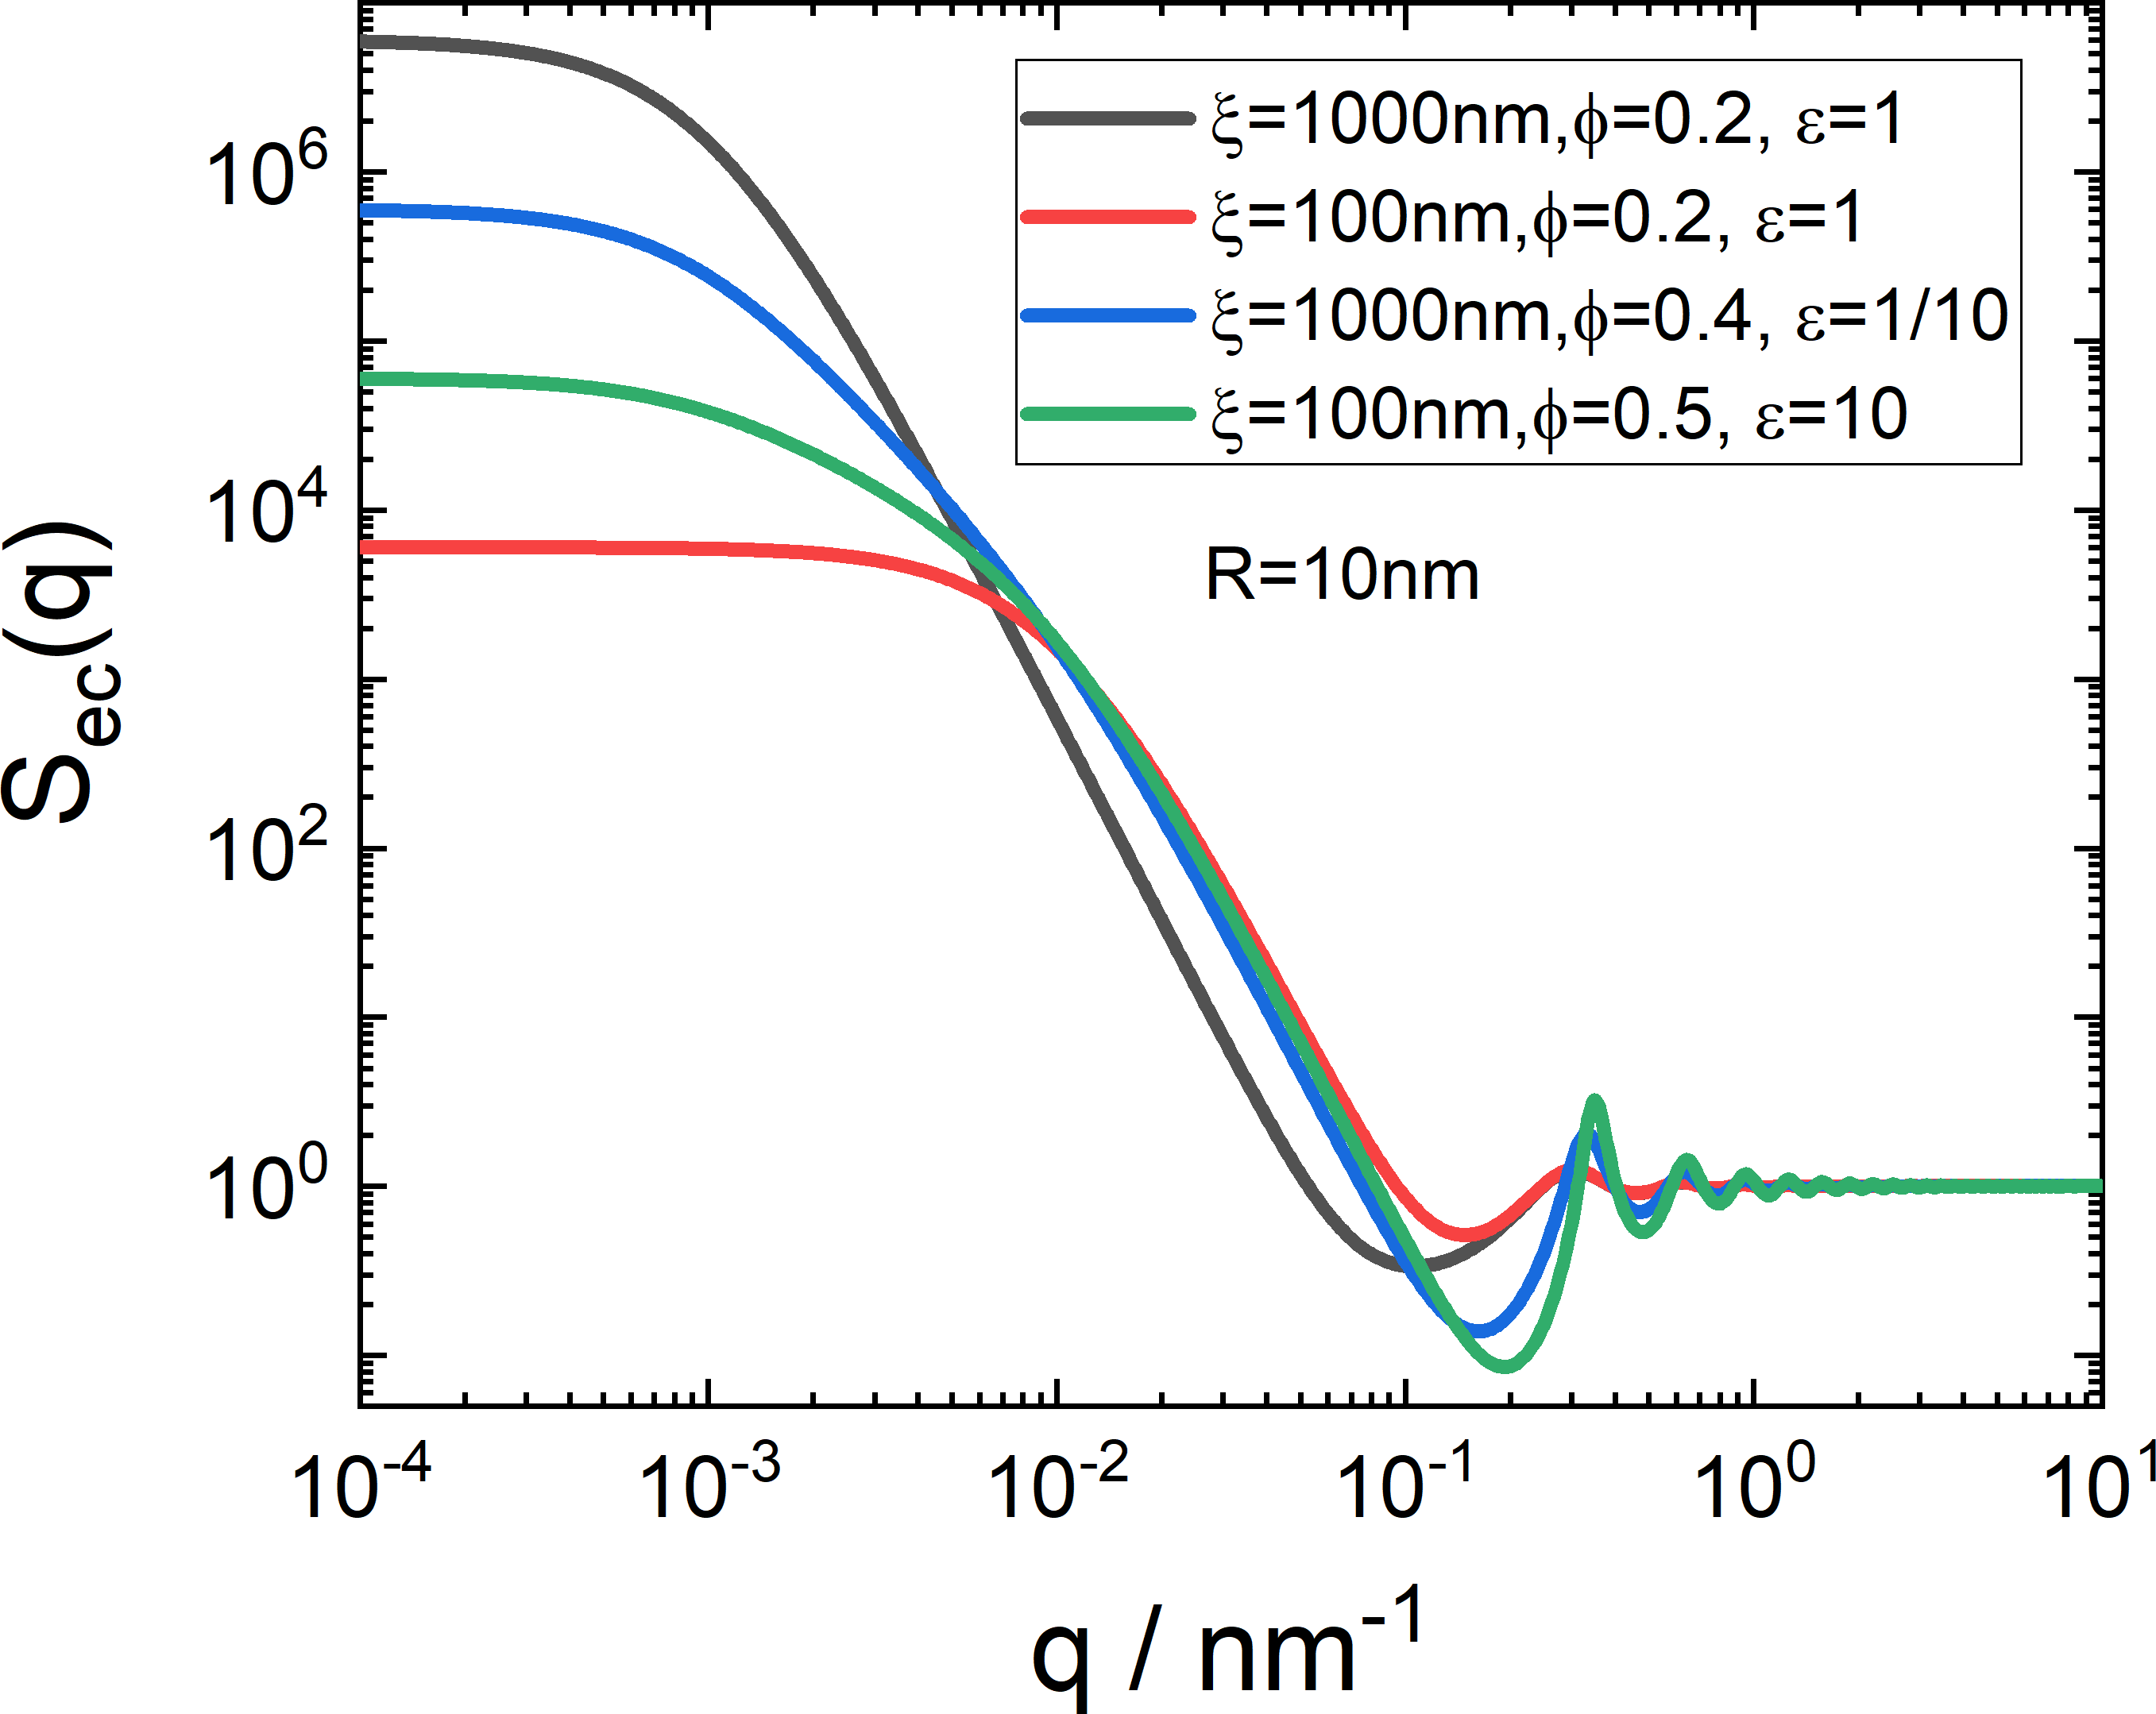
\includegraphics[width=0.55\textwidth]{../images/structure_factor/MassFractals/extendedclusterSQ.png}
\end{center}
\caption{Examples for extended cluster structure factor.}
\label{fig:SQec}
\end{figure}

\noindent \uline{Input Parameters for model \texttt{extended cluster Sq}:}
\begin{description}
\item[\texttt{R}] radius of particles in cluster $R$
\item[\texttt{phi}] local volume fraction inside cluster $\phi$
\item[\texttt{xi}] size (correlation length) of cluster $\xi$
\item[\texttt{epsilon}] shape parameter of cluster (<1:disc; >1:rod) $\epsilon$
\end{description}


\noindent\uline{Note:}
\begin{itemize}
\item the volume fraction needs to be positive and smaller or equal 1:$\phi\in [0,1]$.
\item the correlation length should be significant larger than $R$ to be physical meaningful
\end{itemize} 